% Options for packages loaded elsewhere
\PassOptionsToPackage{unicode}{hyperref}
\PassOptionsToPackage{hyphens}{url}
\PassOptionsToPackage{dvipsnames,svgnames*,x11names*}{xcolor}
%
\documentclass[
]{book}
\usepackage{amsmath,amssymb}
\usepackage{lmodern}
\usepackage{ifxetex,ifluatex}
\ifnum 0\ifxetex 1\fi\ifluatex 1\fi=0 % if pdftex
  \usepackage[T1]{fontenc}
  \usepackage[utf8]{inputenc}
  \usepackage{textcomp} % provide euro and other symbols
\else % if luatex or xetex
  \usepackage{unicode-math}
  \defaultfontfeatures{Scale=MatchLowercase}
  \defaultfontfeatures[\rmfamily]{Ligatures=TeX,Scale=1}
\fi
% Use upquote if available, for straight quotes in verbatim environments
\IfFileExists{upquote.sty}{\usepackage{upquote}}{}
\IfFileExists{microtype.sty}{% use microtype if available
  \usepackage[]{microtype}
  \UseMicrotypeSet[protrusion]{basicmath} % disable protrusion for tt fonts
}{}
\makeatletter
\@ifundefined{KOMAClassName}{% if non-KOMA class
  \IfFileExists{parskip.sty}{%
    \usepackage{parskip}
  }{% else
    \setlength{\parindent}{0pt}
    \setlength{\parskip}{6pt plus 2pt minus 1pt}}
}{% if KOMA class
  \KOMAoptions{parskip=half}}
\makeatother
\usepackage{xcolor}
\IfFileExists{xurl.sty}{\usepackage{xurl}}{} % add URL line breaks if available
\IfFileExists{bookmark.sty}{\usepackage{bookmark}}{\usepackage{hyperref}}
\hypersetup{
  pdftitle={R Programming: Zero to Pro},
  pdfauthor={Yang Feng and Jianan Zhu},
  colorlinks=true,
  linkcolor=Maroon,
  filecolor=Maroon,
  citecolor=Blue,
  urlcolor=Blue,
  pdfcreator={LaTeX via pandoc}}
\urlstyle{same} % disable monospaced font for URLs
\usepackage{color}
\usepackage{fancyvrb}
\newcommand{\VerbBar}{|}
\newcommand{\VERB}{\Verb[commandchars=\\\{\}]}
\DefineVerbatimEnvironment{Highlighting}{Verbatim}{commandchars=\\\{\}}
% Add ',fontsize=\small' for more characters per line
\usepackage{framed}
\definecolor{shadecolor}{RGB}{248,248,248}
\newenvironment{Shaded}{\begin{snugshade}}{\end{snugshade}}
\newcommand{\AlertTok}[1]{\textcolor[rgb]{0.94,0.16,0.16}{#1}}
\newcommand{\AnnotationTok}[1]{\textcolor[rgb]{0.56,0.35,0.01}{\textbf{\textit{#1}}}}
\newcommand{\AttributeTok}[1]{\textcolor[rgb]{0.77,0.63,0.00}{#1}}
\newcommand{\BaseNTok}[1]{\textcolor[rgb]{0.00,0.00,0.81}{#1}}
\newcommand{\BuiltInTok}[1]{#1}
\newcommand{\CharTok}[1]{\textcolor[rgb]{0.31,0.60,0.02}{#1}}
\newcommand{\CommentTok}[1]{\textcolor[rgb]{0.56,0.35,0.01}{\textit{#1}}}
\newcommand{\CommentVarTok}[1]{\textcolor[rgb]{0.56,0.35,0.01}{\textbf{\textit{#1}}}}
\newcommand{\ConstantTok}[1]{\textcolor[rgb]{0.00,0.00,0.00}{#1}}
\newcommand{\ControlFlowTok}[1]{\textcolor[rgb]{0.13,0.29,0.53}{\textbf{#1}}}
\newcommand{\DataTypeTok}[1]{\textcolor[rgb]{0.13,0.29,0.53}{#1}}
\newcommand{\DecValTok}[1]{\textcolor[rgb]{0.00,0.00,0.81}{#1}}
\newcommand{\DocumentationTok}[1]{\textcolor[rgb]{0.56,0.35,0.01}{\textbf{\textit{#1}}}}
\newcommand{\ErrorTok}[1]{\textcolor[rgb]{0.64,0.00,0.00}{\textbf{#1}}}
\newcommand{\ExtensionTok}[1]{#1}
\newcommand{\FloatTok}[1]{\textcolor[rgb]{0.00,0.00,0.81}{#1}}
\newcommand{\FunctionTok}[1]{\textcolor[rgb]{0.00,0.00,0.00}{#1}}
\newcommand{\ImportTok}[1]{#1}
\newcommand{\InformationTok}[1]{\textcolor[rgb]{0.56,0.35,0.01}{\textbf{\textit{#1}}}}
\newcommand{\KeywordTok}[1]{\textcolor[rgb]{0.13,0.29,0.53}{\textbf{#1}}}
\newcommand{\NormalTok}[1]{#1}
\newcommand{\OperatorTok}[1]{\textcolor[rgb]{0.81,0.36,0.00}{\textbf{#1}}}
\newcommand{\OtherTok}[1]{\textcolor[rgb]{0.56,0.35,0.01}{#1}}
\newcommand{\PreprocessorTok}[1]{\textcolor[rgb]{0.56,0.35,0.01}{\textit{#1}}}
\newcommand{\RegionMarkerTok}[1]{#1}
\newcommand{\SpecialCharTok}[1]{\textcolor[rgb]{0.00,0.00,0.00}{#1}}
\newcommand{\SpecialStringTok}[1]{\textcolor[rgb]{0.31,0.60,0.02}{#1}}
\newcommand{\StringTok}[1]{\textcolor[rgb]{0.31,0.60,0.02}{#1}}
\newcommand{\VariableTok}[1]{\textcolor[rgb]{0.00,0.00,0.00}{#1}}
\newcommand{\VerbatimStringTok}[1]{\textcolor[rgb]{0.31,0.60,0.02}{#1}}
\newcommand{\WarningTok}[1]{\textcolor[rgb]{0.56,0.35,0.01}{\textbf{\textit{#1}}}}
\usepackage{longtable,booktabs,array}
\usepackage{calc} % for calculating minipage widths
% Correct order of tables after \paragraph or \subparagraph
\usepackage{etoolbox}
\makeatletter
\patchcmd\longtable{\par}{\if@noskipsec\mbox{}\fi\par}{}{}
\makeatother
% Allow footnotes in longtable head/foot
\IfFileExists{footnotehyper.sty}{\usepackage{footnotehyper}}{\usepackage{footnote}}
\makesavenoteenv{longtable}
\usepackage{graphicx}
\makeatletter
\def\maxwidth{\ifdim\Gin@nat@width>\linewidth\linewidth\else\Gin@nat@width\fi}
\def\maxheight{\ifdim\Gin@nat@height>\textheight\textheight\else\Gin@nat@height\fi}
\makeatother
% Scale images if necessary, so that they will not overflow the page
% margins by default, and it is still possible to overwrite the defaults
% using explicit options in \includegraphics[width, height, ...]{}
\setkeys{Gin}{width=\maxwidth,height=\maxheight,keepaspectratio}
% Set default figure placement to htbp
\makeatletter
\def\fps@figure{htbp}
\makeatother
\setlength{\emergencystretch}{3em} % prevent overfull lines
\providecommand{\tightlist}{%
  \setlength{\itemsep}{0pt}\setlength{\parskip}{0pt}}
\setcounter{secnumdepth}{5}
\usepackage{booktabs}
\usepackage{longtable}
\usepackage[bf,singlelinecheck=off]{caption}

\usepackage{Alegreya}
\usepackage[scale=.8]{sourcecodepro}

\usepackage{framed,color}
\definecolor{shadecolor}{RGB}{248,248,248}

\renewcommand{\textfraction}{0.05}
\renewcommand{\topfraction}{0.8}
\renewcommand{\bottomfraction}{0.8}
\renewcommand{\floatpagefraction}{0.75}

\renewenvironment{quote}{\begin{VF}}{\end{VF}}
\let\oldhref\href
\renewcommand{\href}[2]{#2\footnote{\url{#1}}}

\ifxetex
  \usepackage{letltxmacro}
  \setlength{\XeTeXLinkMargin}{1pt}
  \LetLtxMacro\SavedIncludeGraphics\includegraphics
  \def\includegraphics#1#{% #1 catches optional stuff (star/opt. arg.)
    \IncludeGraphicsAux{#1}%
  }%
  \newcommand*{\IncludeGraphicsAux}[2]{%
    \XeTeXLinkBox{%
      \SavedIncludeGraphics#1{#2}%
    }%
  }%
\fi

\usepackage{makeidx}
\makeindex

\urlstyle{tt}

\usepackage{amsthm}
\makeatletter
\def\thm@space@setup{%
  \thm@preskip=8pt plus 2pt minus 4pt
  \thm@postskip=\thm@preskip
}
\makeatother

\frontmatter
\usepackage{color}
\usepackage{framed}
\setlength{\fboxsep}{.8em}

\newenvironment{blackbox}{
  \definecolor{shadecolor}{rgb}{0, 0, 0}  % black
  \color{white}
  \begin{shaded}}
 {\end{shaded}}
\newenvironment{infobox}[1]
  {
  \begin{itemize}
  \renewcommand{\labelitemi}{
    \raisebox{-.7\height}[0pt][0pt]{
      {\setkeys{Gin}{width=3em,keepaspectratio}
        \includegraphics{pics/#1}}
    }
  }
  \setlength{\fboxsep}{1em}
  \begin{blackbox}
  \item
  }
  {
  \end{blackbox}
  \end{itemize}
  }
\usepackage{booktabs}
\usepackage{longtable}
\usepackage{array}
\usepackage{multirow}
\usepackage{wrapfig}
\usepackage{float}
\usepackage{colortbl}
\usepackage{pdflscape}
\usepackage{tabu}
\usepackage{threeparttable}
\usepackage{threeparttablex}
\usepackage[normalem]{ulem}
\usepackage{makecell}
\usepackage{xcolor}
\ifluatex
  \usepackage{selnolig}  % disable illegal ligatures
\fi
\usepackage[]{natbib}
\bibliographystyle{apalike}

\title{R Programming: Zero to Pro}
\author{Yang Feng and Jianan Zhu}
\date{2021-09-29}

\begin{document}
\maketitle

{
\hypersetup{linkcolor=}
\setcounter{tocdepth}{1}
\tableofcontents
}
\hypertarget{preface}{%
\chapter*{Preface}\label{preface}}
\addcontentsline{toc}{chapter}{Preface}

This book is for anyone who is interested in learning R and Data Science. It is designed for people with zero background in programming.

We also have a companion R package named \textbf{r02pro}, containing the data sets used as well as interactive exercises for each part.

\hypertarget{introduction}{%
\chapter{Introduction}\label{introduction}}

This chapter begins with the installation of R, RStudio, and R Packages in Section \ref{Installation}, and shows how to use R as a fancy calculator in Section \ref{Calculator}.

\hypertarget{Installation}{%
\section{Installation of R, RStudio and R Packages}\label{Installation}}

\hypertarget{download-and-install}{%
\subsection{Download and Install}\label{download-and-install}}

As a first step, you need to download R and RStudio, whose links are as follows. For both software, you need to choose the version that corresponds to your operation system.

Download R: \url{https://cloud.r-project.org/}

Download RStudio: \url{https://rstudio.com/products/rstudio/download/\#download}

RStudio is an \emph{Integrated Development Environment} for R, which is powerful yet easy to use. Throughout this book, you will use RStudio instead of R to learn R programming. Next, let's get started with a quick tour of RStudio.

\hypertarget{rstudio-interface}{%
\subsection{RStudio Interface}\label{rstudio-interface}}

After opening RStudio for the first time, you may find that the font and button size is a bit small. Let's see how to customize the appearance.

\textbf{\emph{a. Customize appearance}}

On the RStudio menu bar, you can click \emph{Tools}, and then click on \emph{Global Options} as shown in the following figure.

\begin{figure}

{\centering 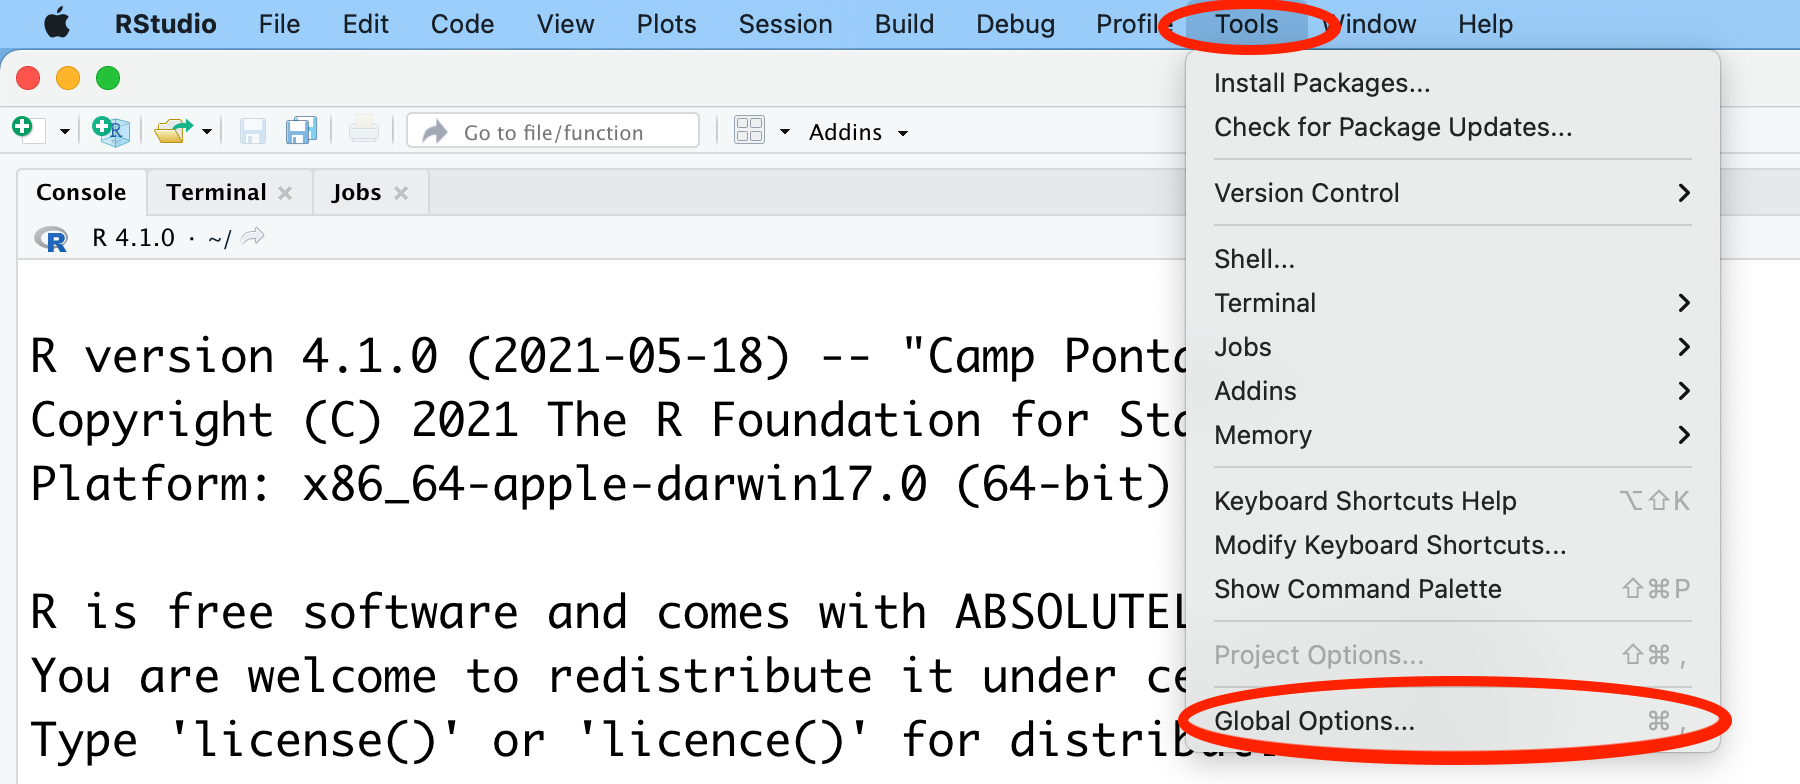
\includegraphics[width=0.9\linewidth]{pics/1font} 

}

\caption{Global Options}\label{fig:font}
\end{figure}

Then, you will see a window pops up like Figure \ref{fig:size}. After clicking on \emph{Appearance}, you can see several drop-down menus including \emph{Zoom} and \emph{Editor font size}, among other choices shown.

\begin{itemize}
\item
  \emph{Zoom} controls the overall scale for all elements in RStudio interface, including the sizes of menu, buttons, as well as the fonts.
\item
  \emph{Editor font size} controls the size of the font only in the code editor.
\end{itemize}

After adjusting the appearance, you need to click on \emph{Apply} to save our settings.

\begin{figure}

{\centering 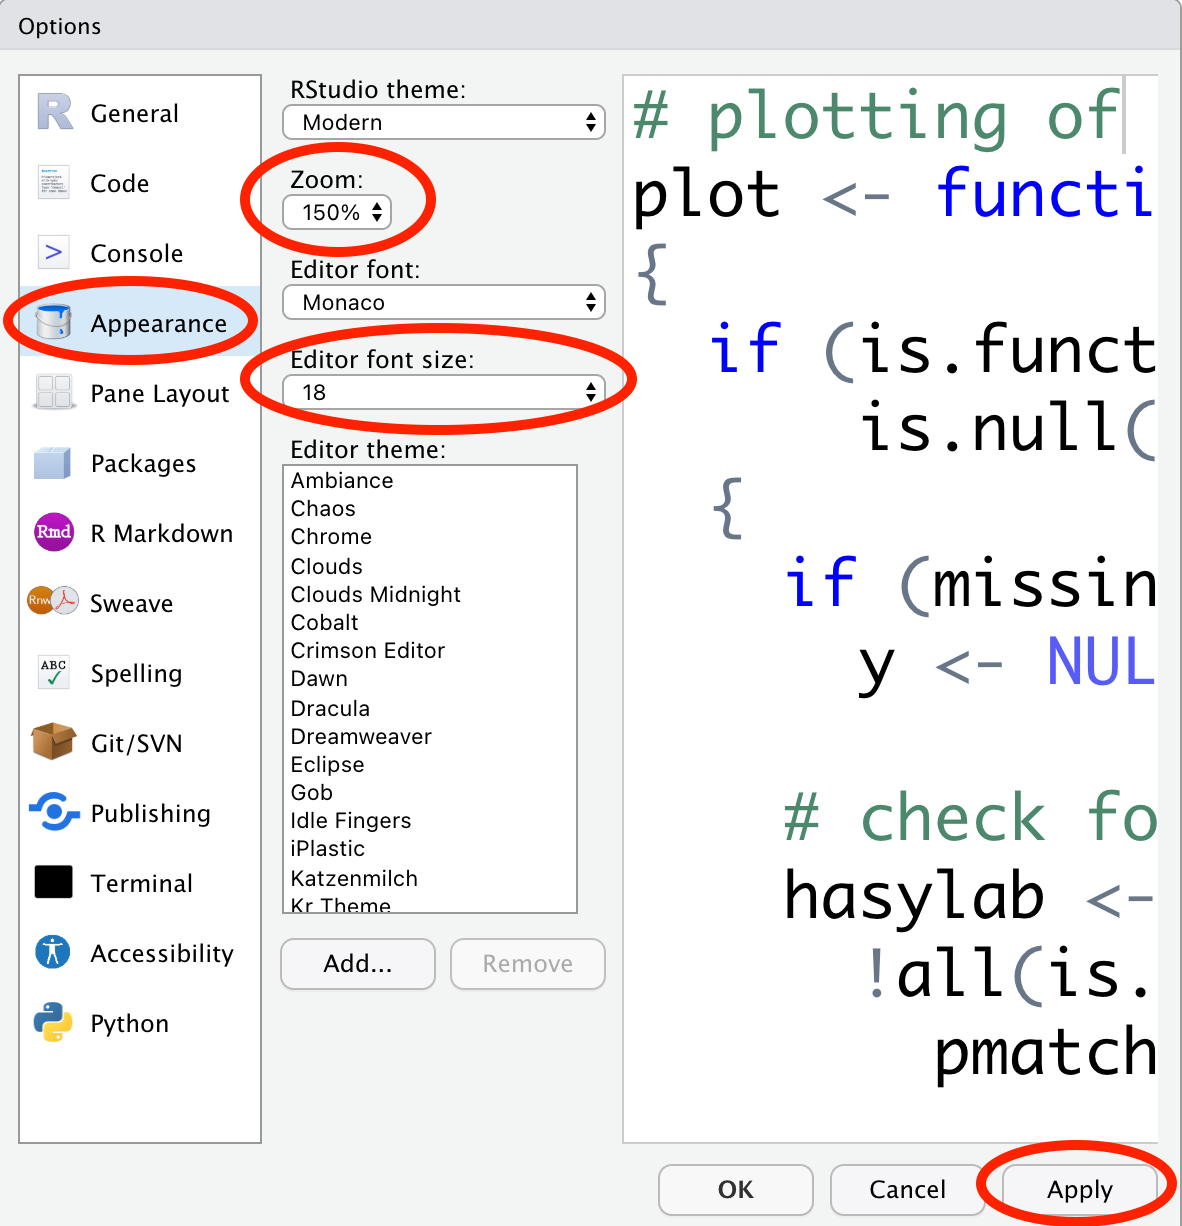
\includegraphics[width=0.7\linewidth]{pics/1size} 

}

\caption{Zoom and Editor font size}\label{fig:size}
\end{figure}

Here, we change the \emph{Zoom} to 150\% and set the \emph{Editor font size} to 18.

\textbf{\emph{b. Four panels of RStudio}}

Now, the RStudio interface is clearer with bigger font size. Although RStudio has four panels, not all of them are visible to us at the beginning (Figure \ref{fig:open}).

\begin{figure}

{\centering 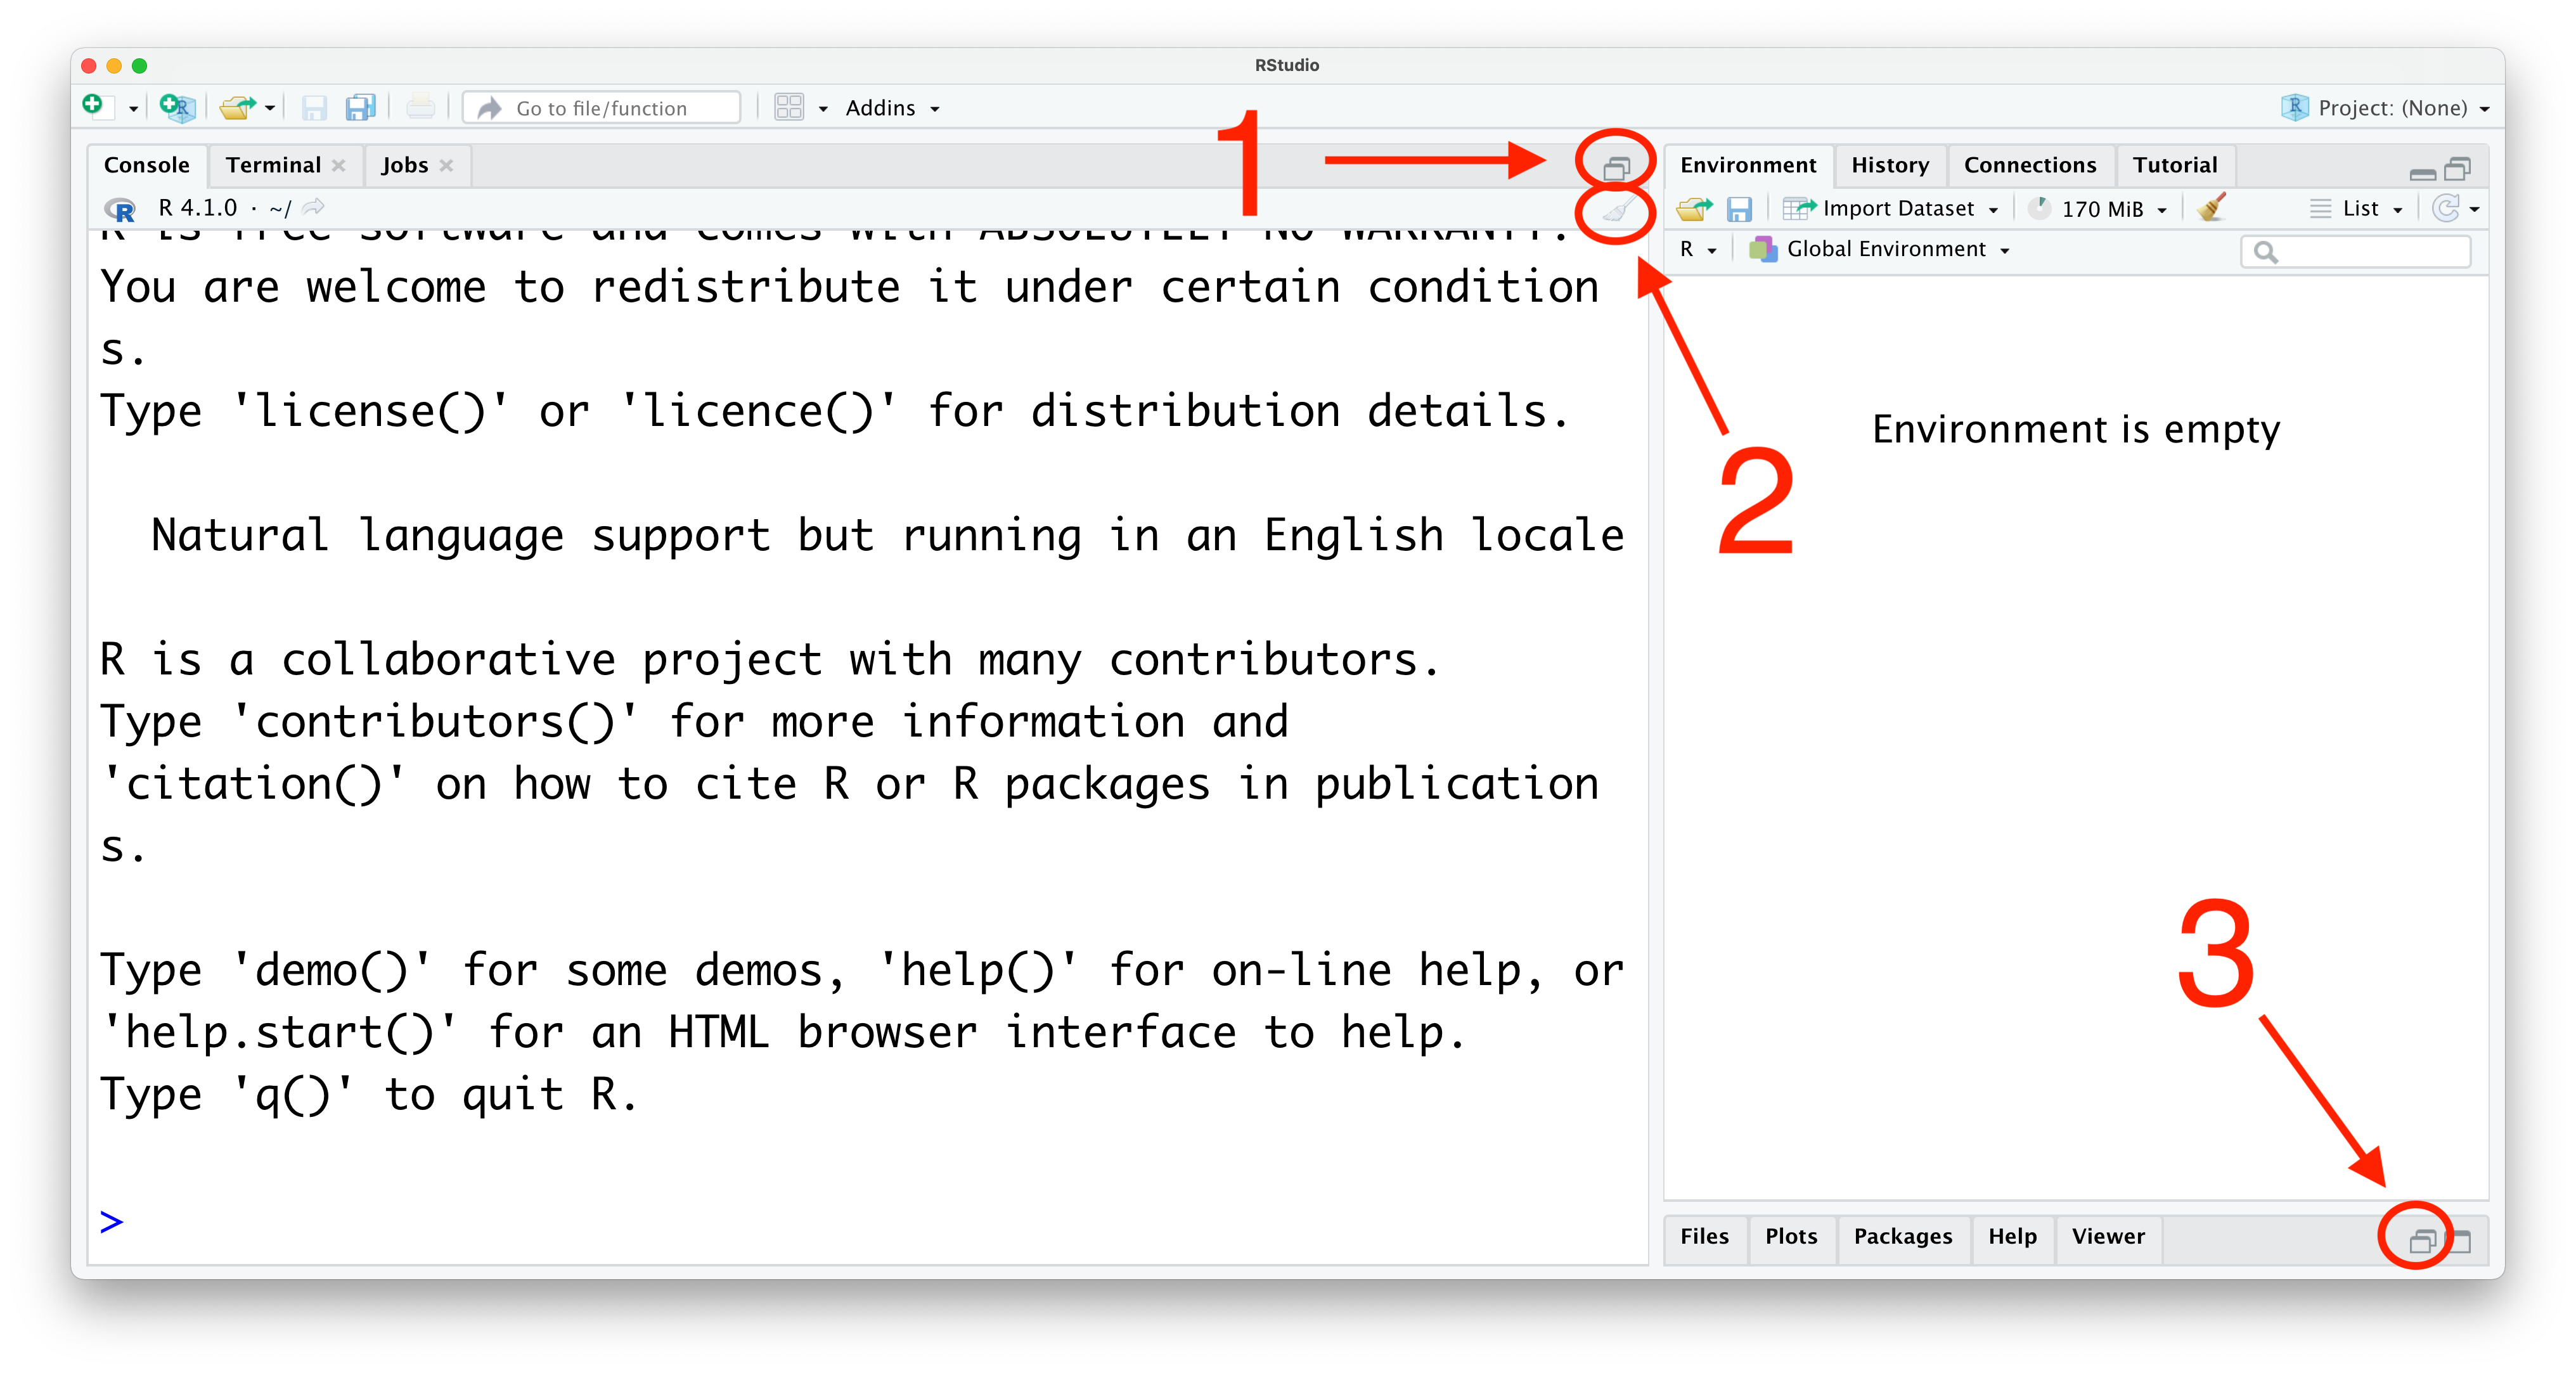
\includegraphics[width=1\linewidth]{pics/1open} 

}

\caption{Unfold panels}\label{fig:open}
\end{figure}

In Figure \ref{fig:open}, we have labeled three useful buttons as 1, 2, and 3. By clicking buttons 1 and 3, you can reveal the two hidden panels. \footnote{Note that you may see different panels hidden when you open RStudio for the first time, depending on the RStudio version. However, you can always reveal the hidden panels by clicking the corresponding buttons like Buttons 1 and 3 in Figure \ref{fig:open}.}
By clicking button 2, we can clear the content in the bottom left panel as shown in the following figure.

\begin{figure}

{\centering 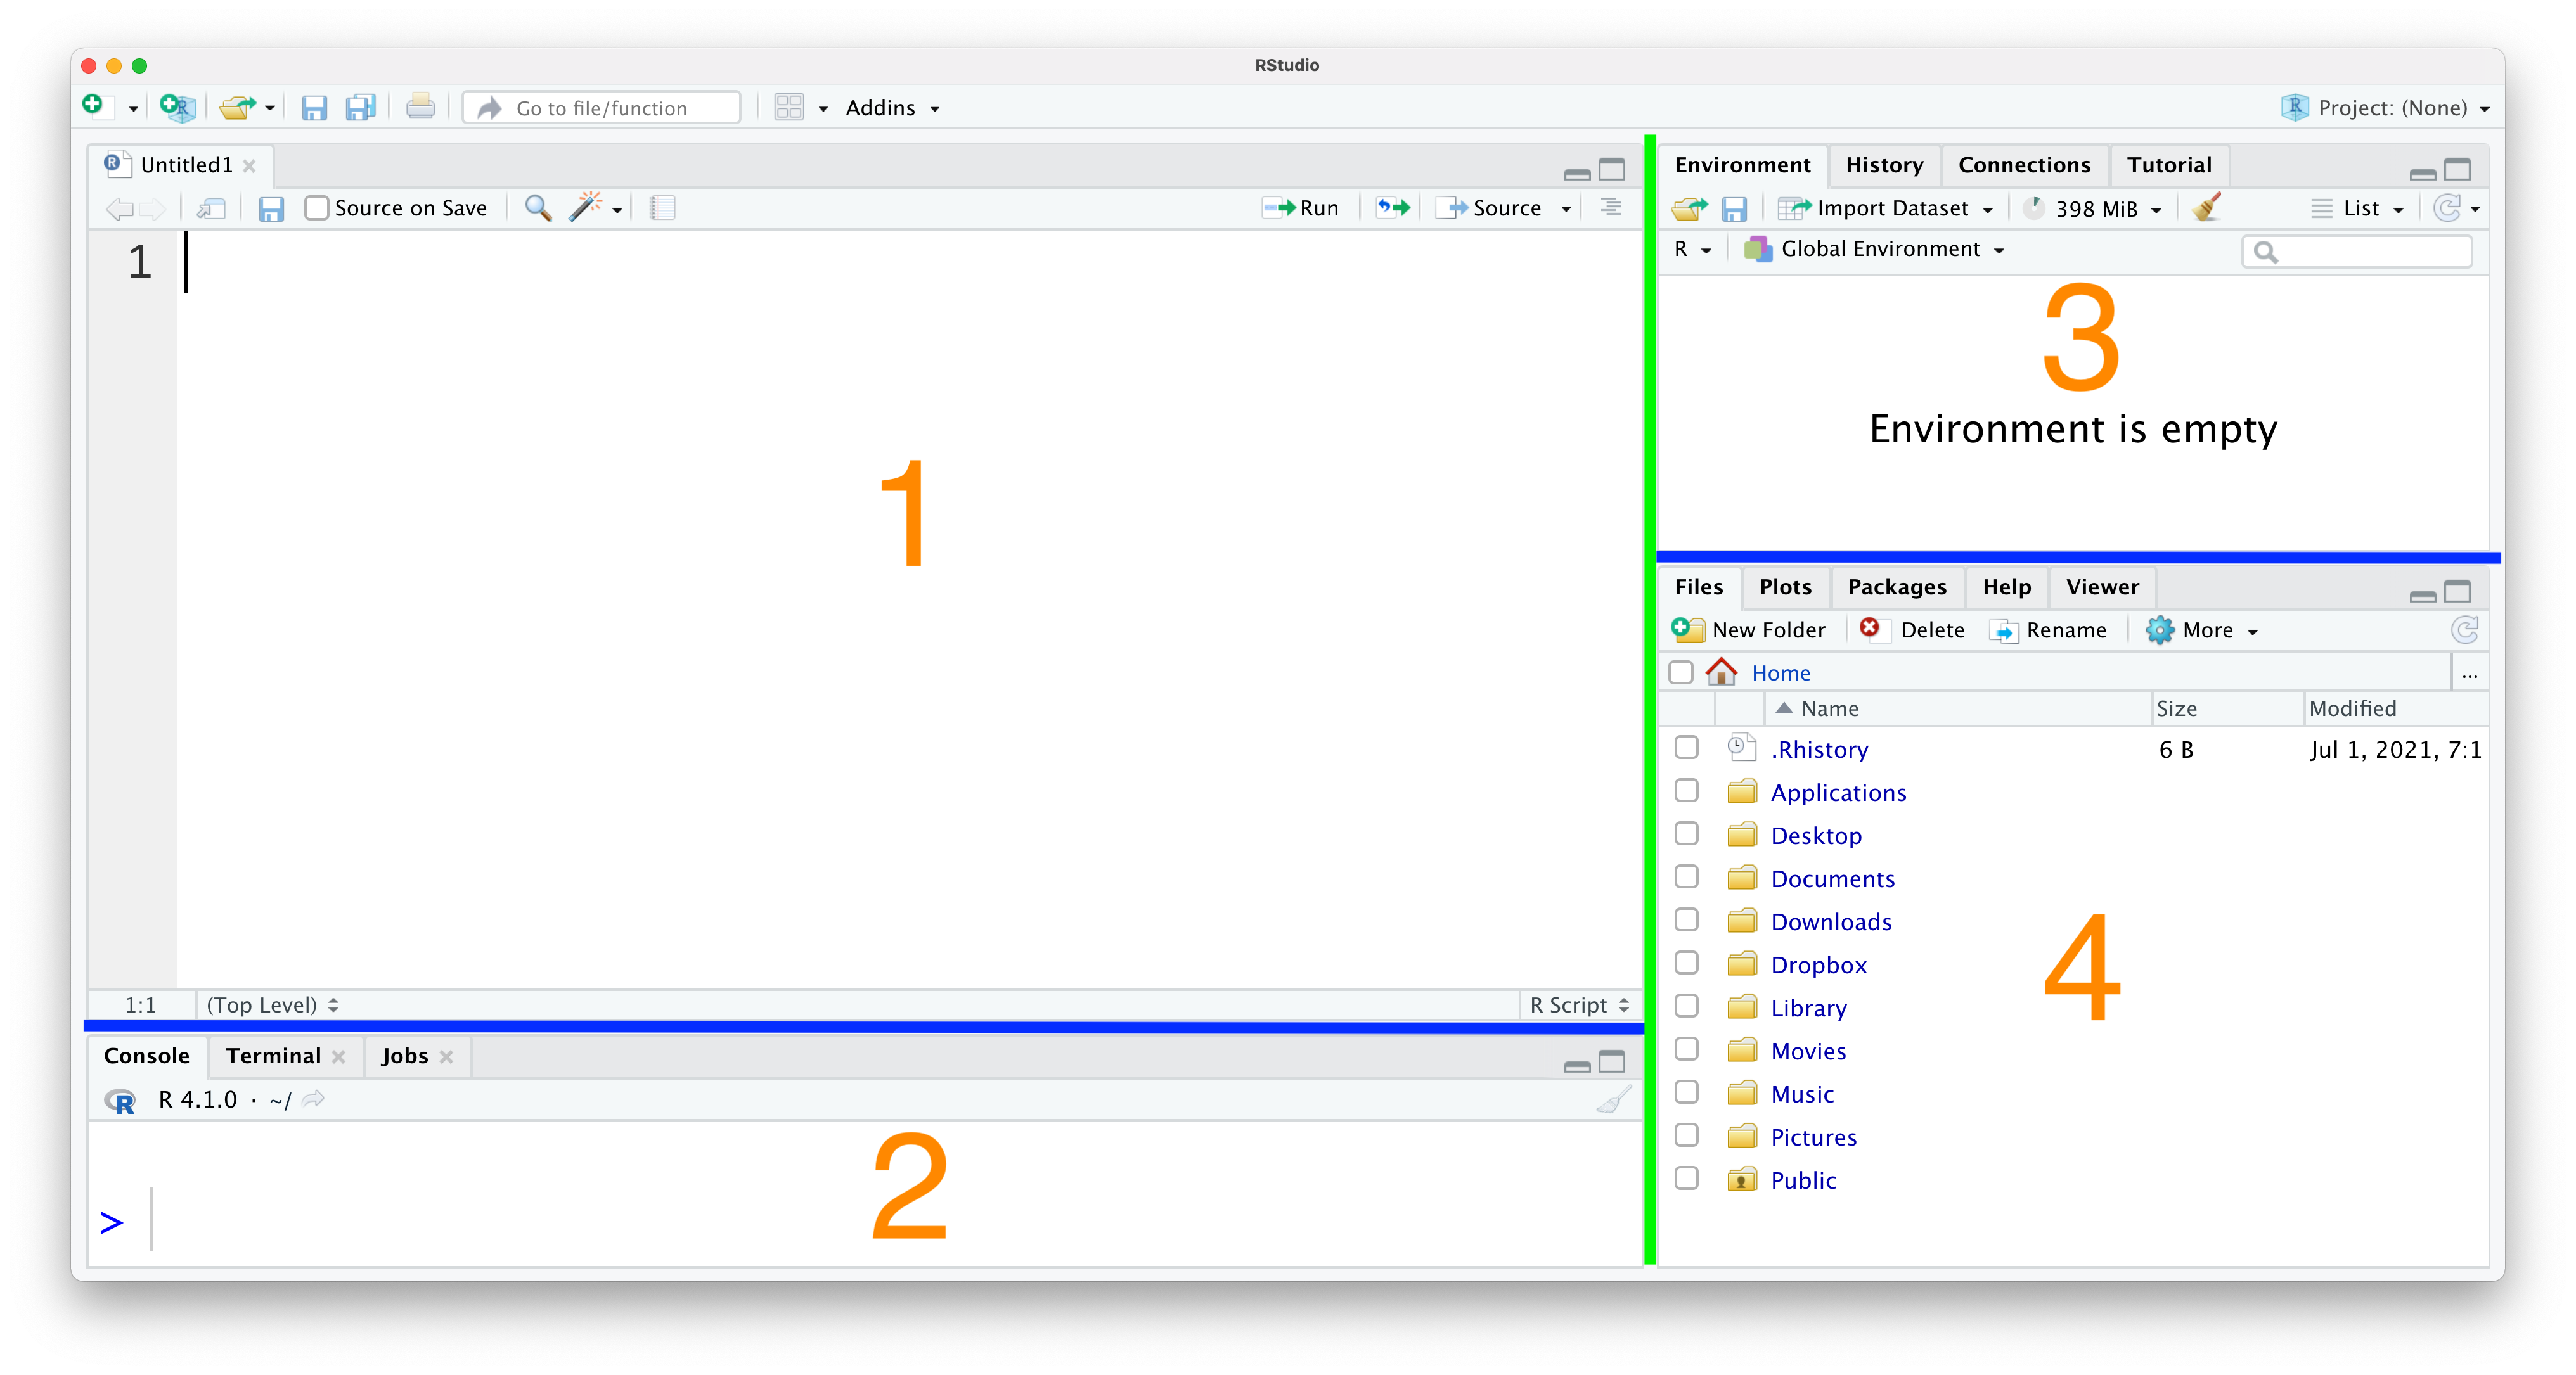
\includegraphics[width=1\linewidth]{pics/1four} 

}

\caption{Four panels}\label{fig:four}
\end{figure}

Now, let's take a close look at all four panels, which are labeled as 1-4 in Figure \ref{fig:four}. You can change the size of each panel by dragging the two blue slides up or down and the green slide left or right.

\begin{itemize}
\item
  Panels 1 and 2 are located to the left of the green line, and are collectively called the \textbf{Code Area}. We will introduce them next.
\item
  Panels 3 and 4 are located to the right of the green line, and are collectively called \textbf{R Support Area}. We will introduce these two panels in later sections. \textbf{Add the section numbers when available}
\end{itemize}

\textbf{\emph{c.~Console}}

Now, let's introduce the panel 2 in Figure \ref{fig:four}, which is usually called the \textbf{Console}.

By clicking the mouse on the line after the \texttt{\textgreater{}} symbol, you can see a blinking cursor, indicating that R is ready to accept codes. Let's type 1 + 2 and press Return (on Mac) or Enter (on Windows).

\begin{infobox}{caution}
It is a good habit to add spaces around an operator to increase readability of the code.

\end{infobox}

\begin{figure}

{\centering 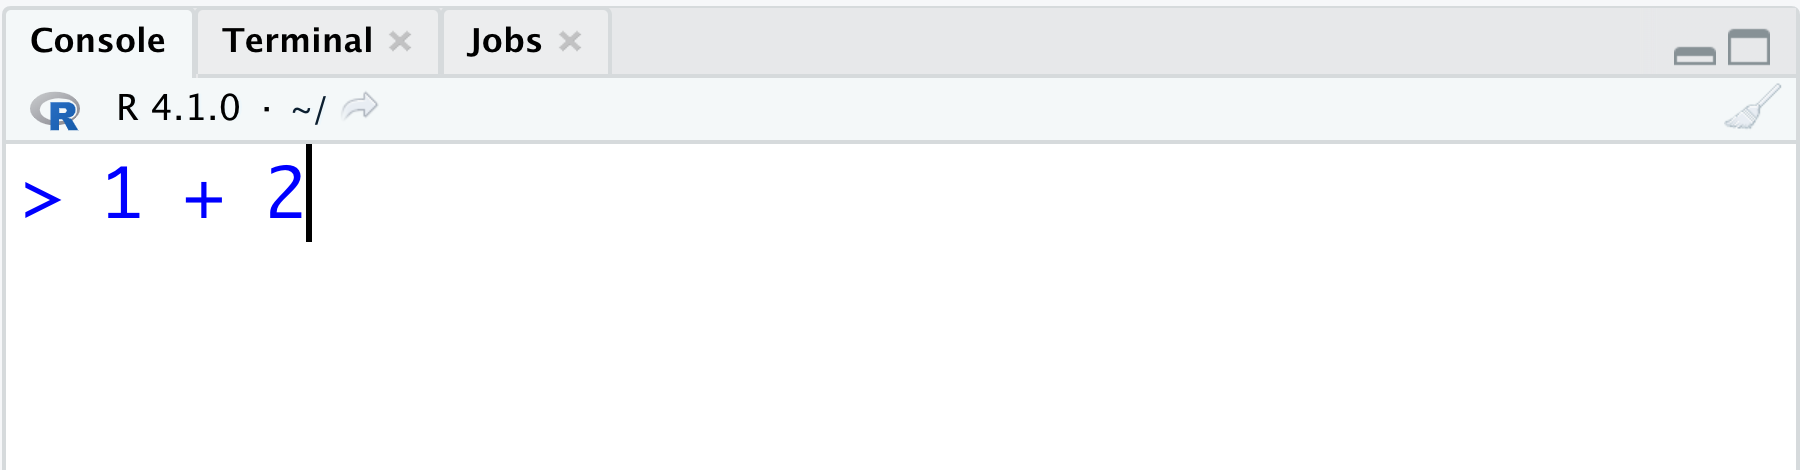
\includegraphics[width=0.7\linewidth]{pics/1code} 

}

\caption{Writing code in the console}\label{fig:code}
\end{figure}

Hooray! You have successfully ran our first piece of R code and gotten the correct answer 3. Note that the blinking cursor now appears on the next line, ready to accept a new line of code.

\begin{figure}

{\centering 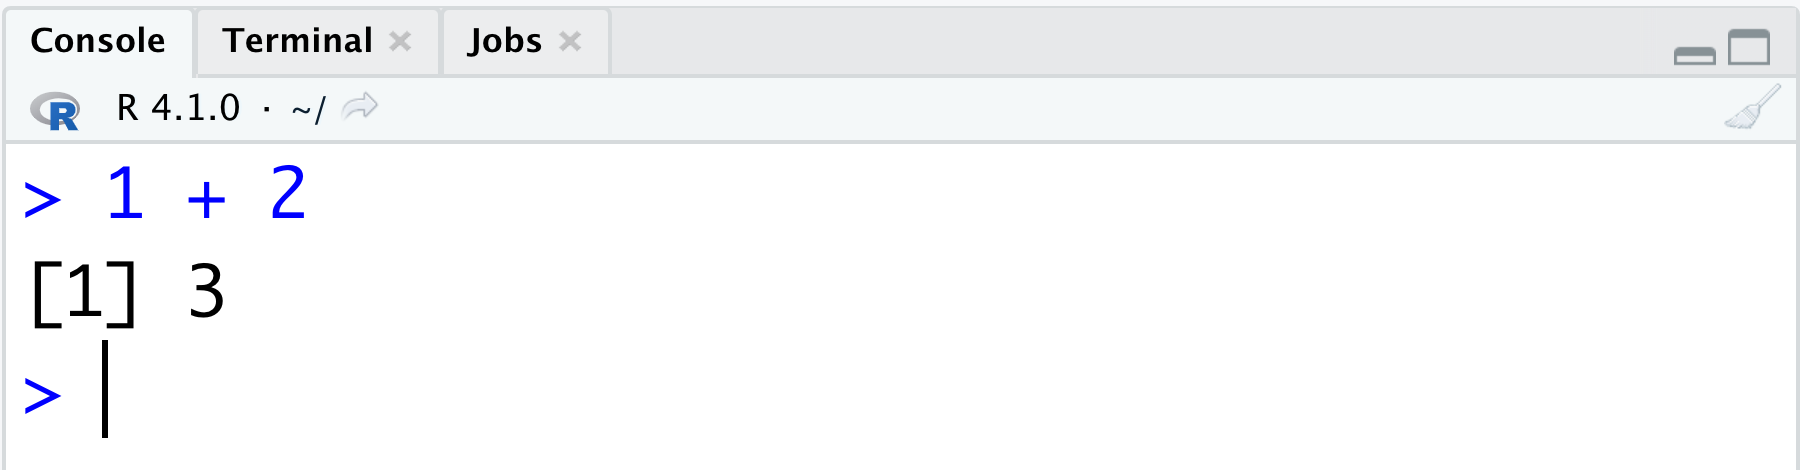
\includegraphics[width=0.7\linewidth]{pics/1answer} 

}

\caption{R code(2)}\label{fig:answer}
\end{figure}

Although the console may work well for some quick calculations, you need to resort to the panel 1 in Figure \ref{fig:four} (usually called the \textbf{Editor}) to save our work and run multiple lines of code at the same time.

\textbf{\emph{d.~Save R codes as scripts}}

The \textbf{Editor} panel is the go-to place to write complicated R codes, which you can save as R scripts for repeated use in the future.

Firstly, we will introduce how to run codes in scripts. Let's go to the editor and type 1 + 2. To run this line of code, you can click the \emph{Run} button. The keyboard shortcut of running this line of code is Cmd+Return on Mac or Ctrl+Enter on Windows.

\begin{figure}

{\centering 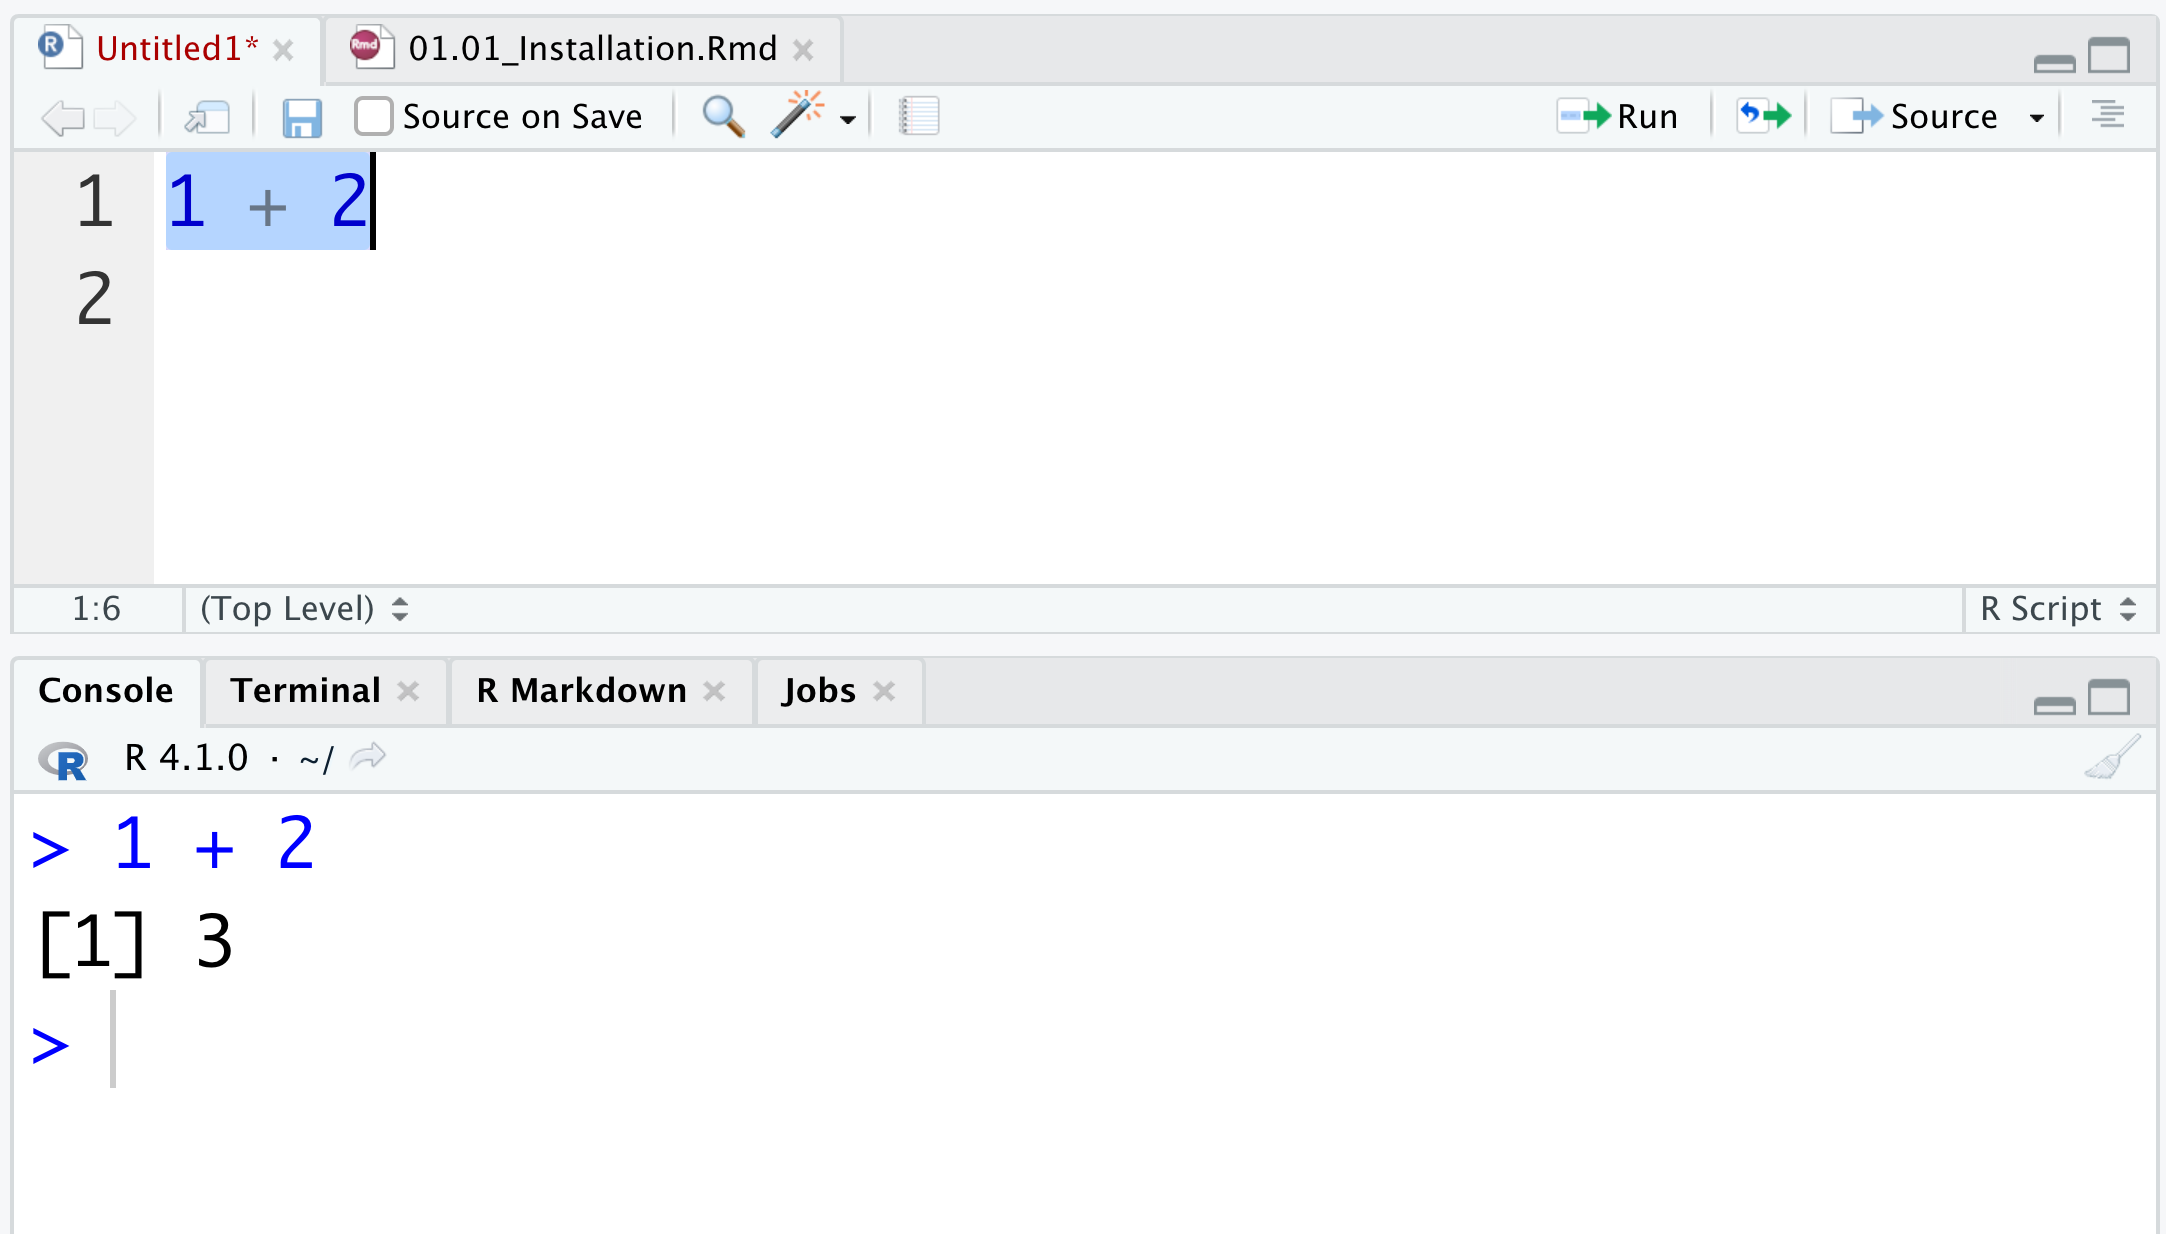
\includegraphics[width=0.7\linewidth]{pics/1run} 

}

\caption{script}\label{fig:run}
\end{figure}

RStudio will then send the line of code to the console and execute the code.

After finishing writing codes in the editor, you can save them as a script. To do that, you can click the \emph{Save} button as shown in the Figure \ref{fig:save1}. The keyboard shortcut of saving files is Cmd+S on Mac or Ctrl+S on Windows.

\begin{figure}

{\centering 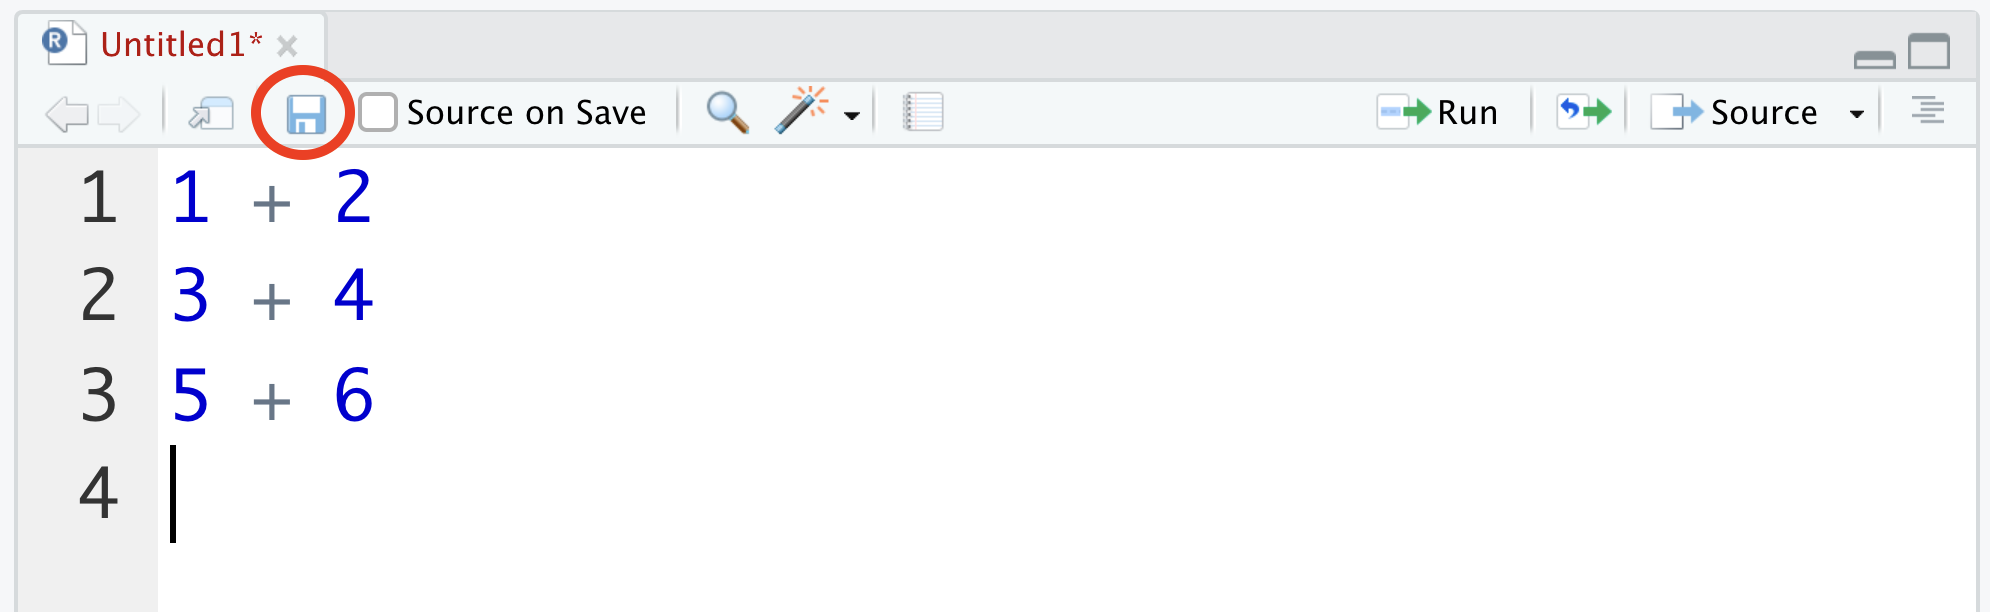
\includegraphics[width=0.7\linewidth]{pics/1save1} 

}

\caption{Save (I)}\label{fig:save1}
\end{figure}

Then you would see a pop-up file dialog box, asking you for a file name and location to save it to. Let's call it lesson1.1 here.

\begin{figure}

{\centering 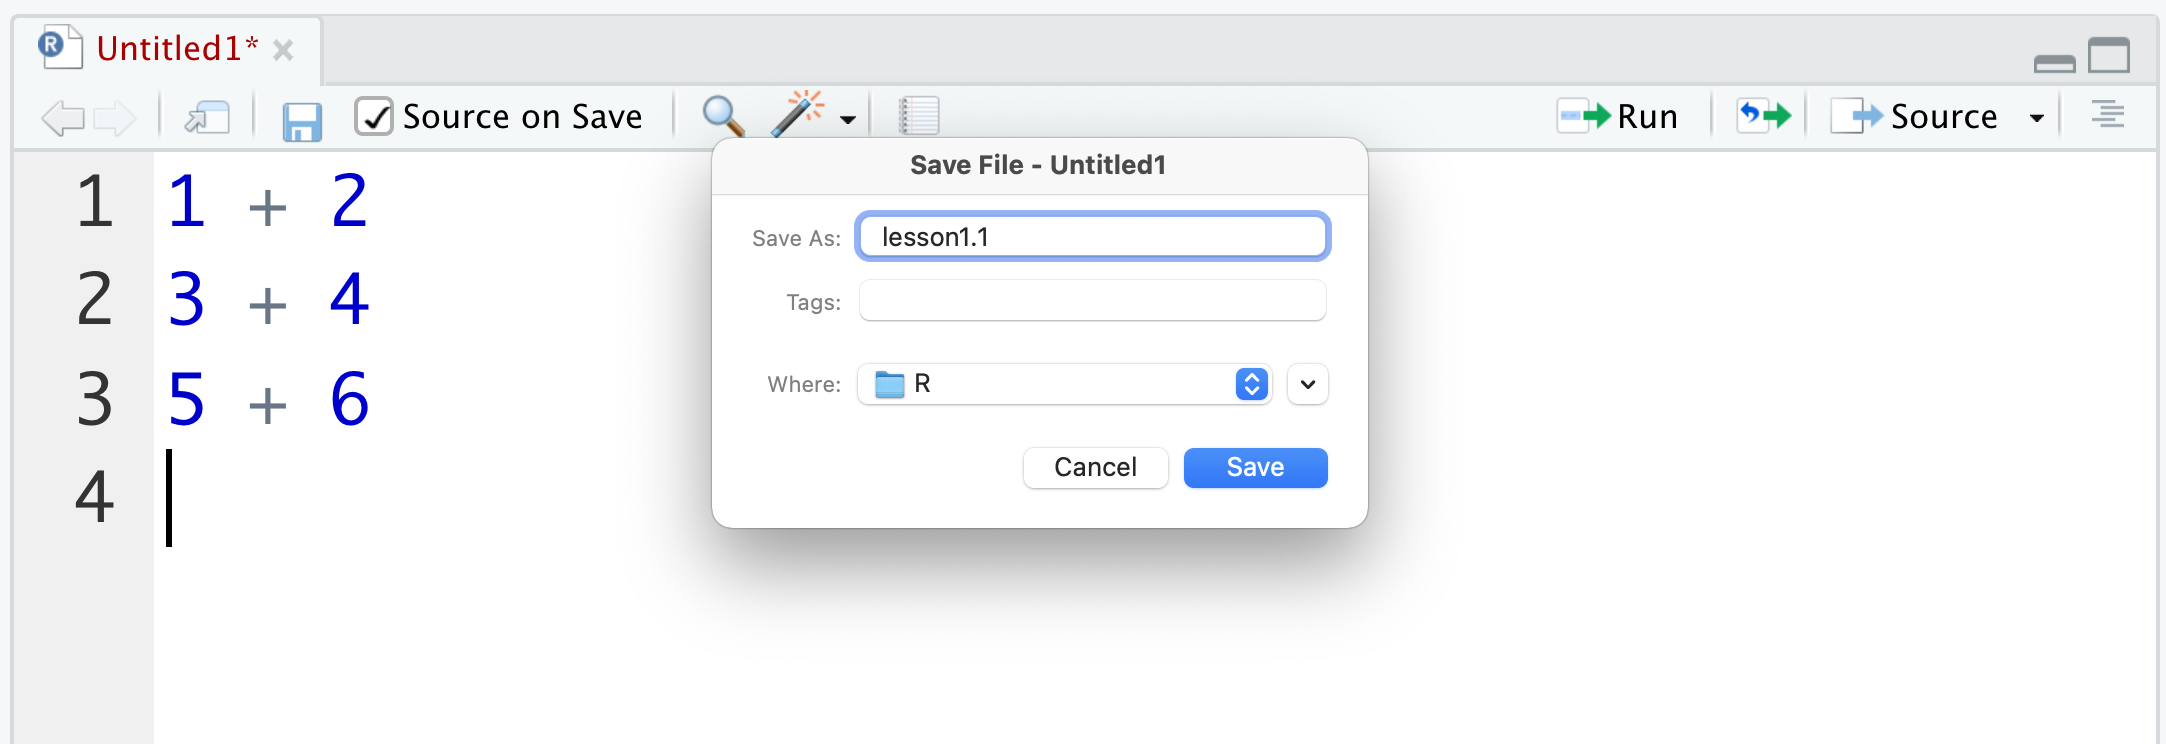
\includegraphics[width=0.7\linewidth]{pics/1save2} 

}

\caption{Save (II)}\label{fig:save2}
\end{figure}

After saving files successfully, you can confirm the name of the R script on the top.

\begin{figure}

{\centering 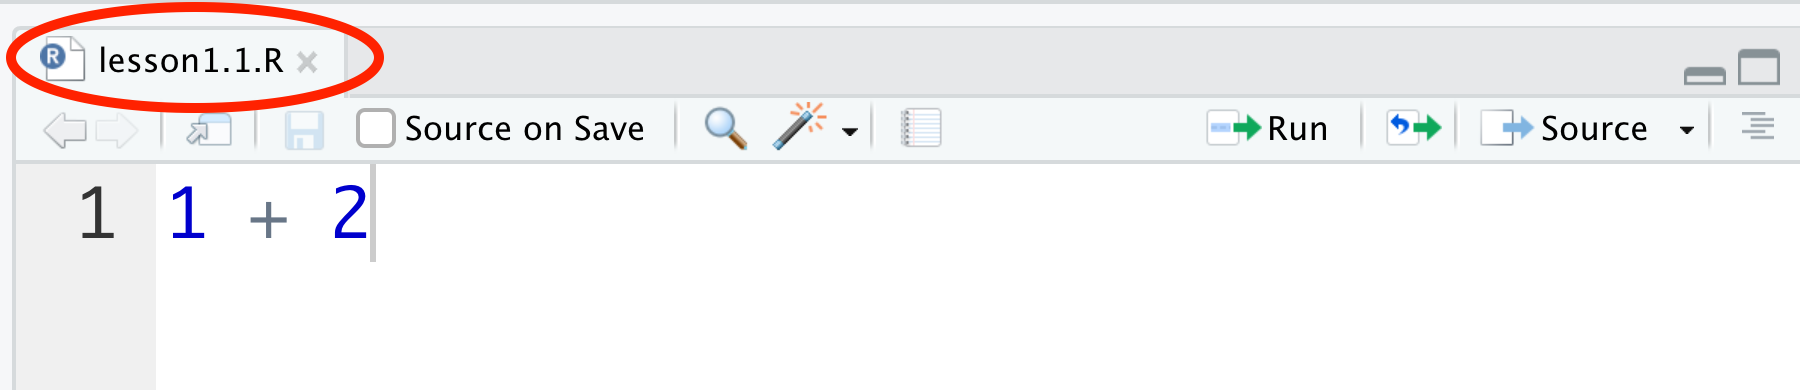
\includegraphics[width=0.7\linewidth]{pics/1save3} 

}

\caption{Save (III)}\label{fig:save3}
\end{figure}

Lastly, if you want to create a new R script, we can click the \texttt{+} button on the menu, then select \emph{R Script}. Note that there are quite a few other options including \emph{R Markdown}, which will be introduced in Section \ref{r-markdown}. Then you will see a new file created.

\begin{figure}

{\centering 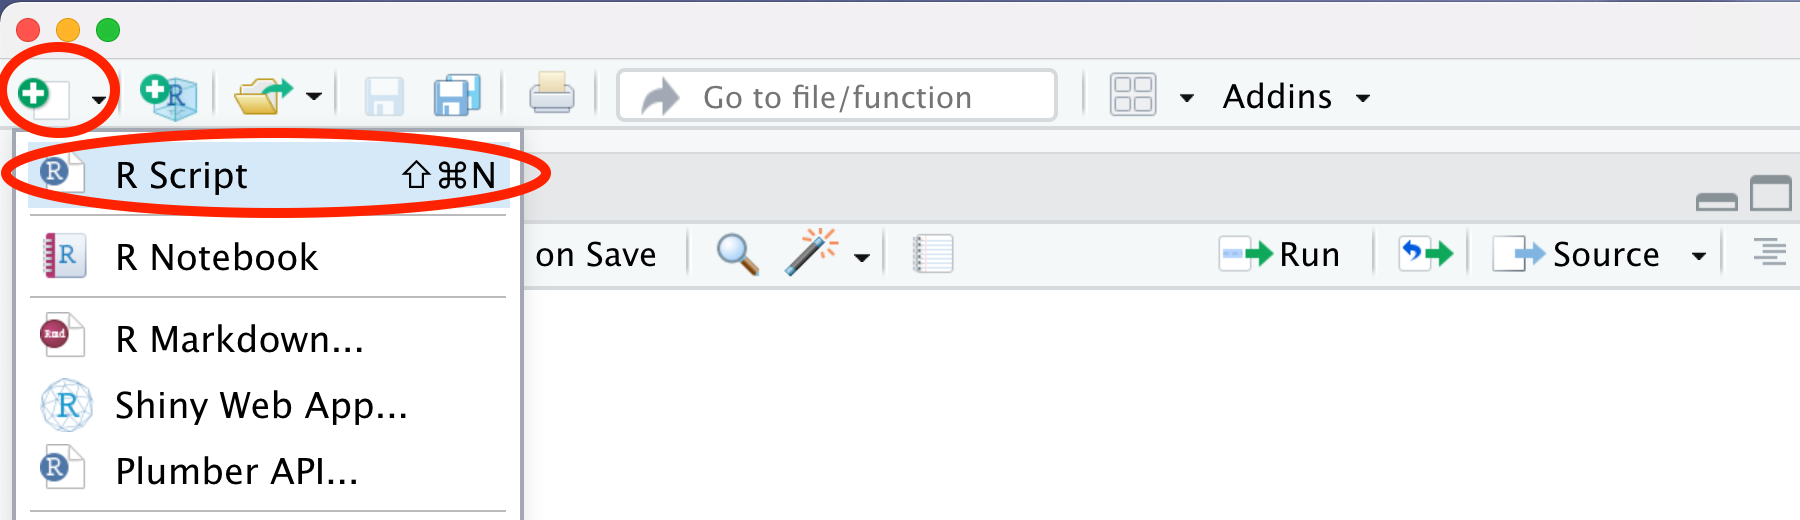
\includegraphics[width=0.7\linewidth]{pics/1new} 

}

\caption{create a new script}\label{fig:new}
\end{figure}

\hypertarget{install-and-load-r-packages}{%
\subsection{Install and load R packages}\label{install-and-load-r-packages}}

Now, you have had a basic understanding of RStudio, it is time to introduce \textbf{R packages}, which greatly extend the capabilities of base R. There are a large number of publicly available R packages. As of July 2021, there are more than 17K R packages on Comprehensive R Archive Network (CRAN), with many others located in Bioconductor, GitHub, and other repositories.

To install an R package, you need to use a built-in R \textbf{function} , which is \texttt{install.packages()}. A \textbf{function} takes in \textbf{arguments} (inputs) and performs a specific task. After the function name, we always need to put \textbf{a pair of parentheses} with the arguments inside.

While there are many built-in R functions, R packages usually contain many useful functions as well, and we can also write our own functions, which will be introduce in Chapter \ref{write-code}.

With \texttt{install.packages()}, the argument is the package name with a pair of quotation marks around it. The task it performs is installing the specific package into R. Here, you will install the companion package for this book, named \texttt{r02pro}, a.k.a. \emph{R Zero to Pro}. The \texttt{r02pro} package contains several data sets that will be used throughout the book, and interactive exercises for each subsection.

\begin{Shaded}
\begin{Highlighting}[]
\FunctionTok{install.packages}\NormalTok{(}\StringTok{"r02pro"}\NormalTok{)}
\end{Highlighting}
\end{Shaded}

\begin{infobox}{caution}
If you miss the right parenthesis, R will show a plus on the next line (as shown in Figure \ref{fig:right1}), waiting for more input to complete the command. If this happens, you can either enter the right parenthesis, or press ESC to escape this command. When you see a blinking cursor after the \texttt{\textgreater{}} symbol, you can write new codes again.

\end{infobox}

\begin{figure}

{\centering 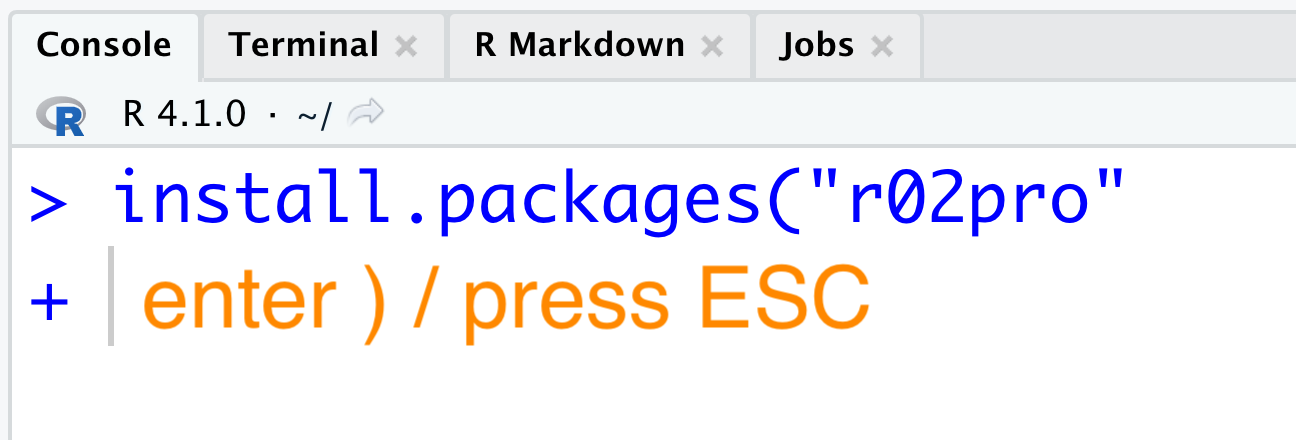
\includegraphics[width=0.7\linewidth]{pics/1right} 

}

\caption{Miss the right parenthesis}\label{fig:right1}
\end{figure}

After a package is installed, you still need to load it into R before using it. To load a package, we use the \texttt{library()} function with the package name as its argument. Here, the quotation marks are not necessary.

\begin{Shaded}
\begin{Highlighting}[]
\FunctionTok{library}\NormalTok{(r02pro)}
\end{Highlighting}
\end{Shaded}

Note that once a package is installed, you don't need to install it again on the same machine. However, when starting a new R session, you would need to load the package again.

\begin{infobox}{caution}

Quotation marks are necessary for installing R packages, but are not necessary for loading packages. If we install packages without quotation marks. We will see an error message, showing \emph{object not found}.

\begin{Shaded}
\begin{Highlighting}[]
\FunctionTok{install.packages}\NormalTok{(r02pro)}
\end{Highlighting}
\end{Shaded}

\end{infobox}

\hypertarget{exercises}{%
\subsection{Exercises}\label{exercises}}

\begin{enumerate}
\def\labelenumi{\arabic{enumi}.}
\tightlist
\item
  Which of the following code using to install packages into R will cause an error?
\end{enumerate}

\begin{itemize}
\tightlist
\item
  \texttt{install.packages("r02pro")}
\item
  \texttt{install.packages(r02pro)}
\end{itemize}

\begin{enumerate}
\def\labelenumi{\arabic{enumi}.}
\setcounter{enumi}{1}
\item
  Write R code to load the package \textbf{r02pro}
\item
  Write R code to calculate \texttt{2\ +\ 3}.
\end{enumerate}

\hypertarget{Calculator}{%
\section{Use R as a Fancy Calculator}\label{Calculator}}

While R is super powerful, it is, first of all, a very fancy calculator.

\hypertarget{add-comments-using}{%
\subsection{Add comments using ``\#''}\label{add-comments-using}}

The first item we will cover is about adding comments. In R, you can add comments using the pound sign \texttt{\#}. In each line, anything after \texttt{\#} are comments, which will be ignored by R. Let's see an example,

\begin{Shaded}
\begin{Highlighting}[]
\DecValTok{6} \SpecialCharTok{{-}} \DecValTok{1} \SpecialCharTok{/} \DecValTok{2} \CommentTok{\#first calculate 1/2=0.5, then 6{-}0.5=5.5}
\CommentTok{\#\textgreater{} [1] 5.5}
\end{Highlighting}
\end{Shaded}

Just looking at the resulting value 5.5, you may not know the detail of the calculation process. The comment informs you the operation order: the division is calculated before the subtraction.

In general, adding comments to codes is a very good practice, as it greatly increases readability and make collaboration easier. We will also add many comments in our codes to help you learn R.

\hypertarget{basic-calculation}{%
\subsection{Basic calculation}\label{basic-calculation}}

Now let's start to use R as a calculator! You can use R to do addition, subtraction, multiplication,division, and combine multiple basic operations. You can also calculate the square root, absolute value and the sign of a number.

\begin{tabular}{l|l}
\hline
Operation & Explanation\\
\hline
1 + 2 & addition\\
\hline
1 - 2 & subtraction\\
\hline
2 * 4 & multiplication\\
\hline
2 / 4 & division\\
\hline
6 - 1 / 2 & multiple operations\\
\hline
sqrt(100) & square root\\
\hline
abs(-3) & absolute value\\
\hline
sign(-3) & sign\\
\hline
\end{tabular}

While the first seven operations in the table look intuitive, you may be wondering, what does the \texttt{sign()} function mean here? Is it a stop sign?

\begin{center}
\includegraphics[width=0.16\linewidth]{pics/1stop} \end{center}

Sometimes, you may have no idea how a particular function works. Fortunately, R provides a detailed documentation for each function. There are three ways to ask for help in R.

\begin{itemize}
\tightlist
\item
  Use question mark followed by the function name, e.g.~\texttt{?sign}\\
\item
  Use help function, e.g.~\texttt{help(sign)}
\item
  Use the help window in RStudio, as shown in Figure \ref{fig:help}. The help window is the panel 4 of Figure \ref{fig:four} in Section \ref{Installation}. Then type in the function name in the box to the right of the magnifying glass and press return.
\end{itemize}

\begin{figure}

{\centering 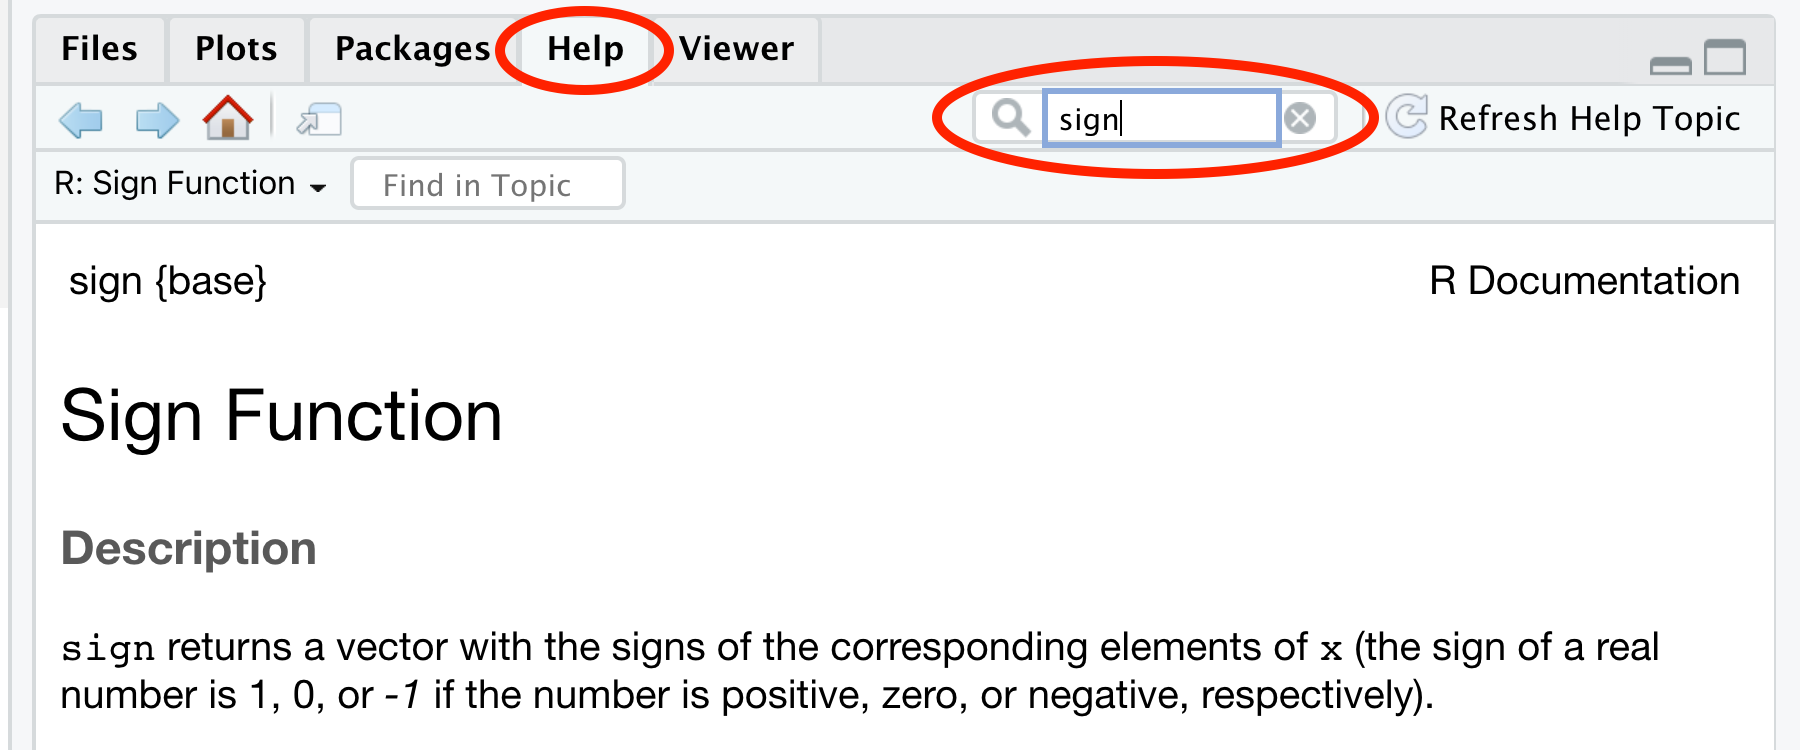
\includegraphics[width=0.7\linewidth]{pics/1help} 

}

\caption{Ask for help}\label{fig:help}
\end{figure}

\hypertarget{approximation}{%
\subsection{Approximation}\label{approximation}}

After learning about doing basic calculations, let's move on to do approximation in R. When you do division, for example, when computing \texttt{7\ /\ 3}, the answer is not a whole number since 7 is not divisible by 3. Under these circumstances, approximation operators are very handy to use. Let's take \texttt{7\ /\ 3} as the example.

\textbf{\emph{a. Get the integer part and the remainder}}

\begin{tabular}{l|l}
\hline
Code & Name\\
\hline
7\%/\%3 = 2 & integer division\\
\hline
7\%\%3 = 1 & modulus\\
\hline
\end{tabular}

We all know that 7 = 3 * \textbf{2} + \textbf{1}. So the \emph{integer division} will pick up the integer part, which is 2 here; and the \emph{modulus} will get the remainder, which is 1.

\textbf{\emph{b. Get the nearby integer}}

\begin{Shaded}
\begin{Highlighting}[]
\FunctionTok{floor}\NormalTok{(}\DecValTok{7} \SpecialCharTok{/} \DecValTok{3}\NormalTok{)   }
\FunctionTok{ceiling}\NormalTok{(}\DecValTok{7} \SpecialCharTok{/} \DecValTok{3}\NormalTok{) }
\end{Highlighting}
\end{Shaded}

Since \textbf{2} \textless= 7/3 \textless= \textbf{3}, you can use the \texttt{floor} function to find the \emph{largest integer} \textless= 7/3, which is 2; and the \texttt{ceiling} function gives the \emph{smallest integer} \textgreater= 7/3, which is 3.

\textbf{\emph{c.~Round to the nearest number}}

\begin{Shaded}
\begin{Highlighting}[]
\FunctionTok{round}\NormalTok{(}\DecValTok{7} \SpecialCharTok{/} \DecValTok{3}\NormalTok{)   }
\FunctionTok{round}\NormalTok{(}\DecValTok{7} \SpecialCharTok{/} \DecValTok{3}\NormalTok{, }\AttributeTok{digits =} \DecValTok{3}\NormalTok{)}
\end{Highlighting}
\end{Shaded}

The \texttt{round} function follows the \textbf{rounding principle}. By default, you will get the nearest integer to \texttt{7\ /\ 3}, which is \texttt{2}. If you want to control the approximation accuracy, you can add a \texttt{digits} argument to specify how many digits you want after the decimal point. Here you will get \texttt{2.333} after adding \texttt{digits\ =\ 3}.

\hypertarget{power-logarithm}{%
\subsection{Power \& logarithm}\label{power-logarithm}}

You can also use R to do \emph{power} and \emph{logarithmic} operations.

Generally, you can use \textbf{\^{}} to do power operations. For example, \texttt{10\^{}5} will give us 10 to the power of 5. Here, 10 is the \emph{base} value, and 5 is the \emph{exponent}. The result is 100000, but it is shown as \texttt{1e+05} in R. That's because R uses the so-called \emph{scientific notation}.

\begin{infobox}{caution}
\textbf{scientific notation}: a common way to express numbers which are too large or too small to be conveniently written in decimal form. Generally, it expresses numbers in forms of \(m \times 10^n\) and R uses the \textbf{e notation}. Note that the \textbf{e notation} has nothing to do with the natural number \(e\). Let's see some examples,
\begin{align}
1 \times 10^5 &= \mbox{1e+05}\\
2 \times 10^4 &= \mbox{2e+04}\\
1.2 \times 10^{-3} &= \mbox{1.2e-03}
\end{align}

\end{infobox}

In mathematics, the \emph{logarithmic operations} are inverse to the power operations. If \textbf{\(b^y = x\)} and you only know \emph{\(b\)} and \emph{\(x\)}, you can do logarithm operations to solve \emph{\(y\)} using the general form \textbf{\(y = \log(x, b)\)}, which is called the logarithm of \(x\) with base \(b\).

In R, logarithm functions with base value of 10, 2, or the natural number \(e\) have shortcuts \texttt{log10()}, \texttt{log2()}, and \texttt{log()}, respectively. Let's see an example of \texttt{log10()}, the logarithm function with base \emph{10}.

\begin{Shaded}
\begin{Highlighting}[]
\DecValTok{10}\SpecialCharTok{\^{}}\DecValTok{6} 
\FunctionTok{log10}\NormalTok{(}\FloatTok{1e6}\NormalTok{) }\CommentTok{\#log10(x) = log(x, 10)}
\end{Highlighting}
\end{Shaded}

Next, let's see \texttt{log2()}, the logarithm function with base \emph{2}.

\begin{Shaded}
\begin{Highlighting}[]
\DecValTok{2}\SpecialCharTok{\^{}}\DecValTok{10}
\FunctionTok{log2}\NormalTok{(}\DecValTok{1024}\NormalTok{)  }\CommentTok{\#log2(x) = log(x, 2)}
\end{Highlighting}
\end{Shaded}

Before moving on to the natural logarithm, note that the natural number \(e\) needs to be written as \texttt{exp(1)} in R. When you want to do power operations on \(e\), you can simply change the argument in the function \texttt{exp()}, for example, \texttt{exp(3)} is \(e\) to the power of 3. Here, \texttt{log()} without specifying the \texttt{base} argument represents the logarithm function with base \(e\).

\begin{Shaded}
\begin{Highlighting}[]
\FunctionTok{exp}\NormalTok{(}\DecValTok{1}\NormalTok{)      }
\FunctionTok{exp}\NormalTok{(}\DecValTok{3}\NormalTok{)}
\FunctionTok{log}\NormalTok{(}\FunctionTok{exp}\NormalTok{(}\DecValTok{3}\NormalTok{))  }\CommentTok{\#log(x) = log(x, exp(1))}
\end{Highlighting}
\end{Shaded}

\hypertarget{trigonometric-function}{%
\subsection{Trigonometric function}\label{trigonometric-function}}

R also provides the common trigonometric functions.

\begin{Shaded}
\begin{Highlighting}[]
\FunctionTok{cos}\NormalTok{(pi)}
\FunctionTok{acos}\NormalTok{(}\SpecialCharTok{{-}}\DecValTok{1}\NormalTok{)}
\end{Highlighting}
\end{Shaded}

Here, \texttt{acos()} is the inverse function of \texttt{cos()}. If we set \(cos(a) = b\), then we will get \(acos(b) = a\).

\begin{Shaded}
\begin{Highlighting}[]
\FunctionTok{sin}\NormalTok{(pi}\SpecialCharTok{/}\DecValTok{2}\NormalTok{)}
\FunctionTok{asin}\NormalTok{(}\DecValTok{1}\NormalTok{)}
\end{Highlighting}
\end{Shaded}

Similarly, \texttt{asin()} is the inverse function of \texttt{sin()}. If we set \(sin(a) = b\), then we will get \(asin(b) = a\).

\begin{Shaded}
\begin{Highlighting}[]
\FunctionTok{tan}\NormalTok{(pi}\SpecialCharTok{/}\DecValTok{4}\NormalTok{)}
\FunctionTok{atan}\NormalTok{(}\DecValTok{1}\NormalTok{)}
\end{Highlighting}
\end{Shaded}

Also, \texttt{atan()} is the inverse function of \texttt{tan()}. If we set \(tan(a) = b\), then we will get \(atan(b) = a\).

\hypertarget{exercises-1}{%
\subsection{Exercises}\label{exercises-1}}

\begin{enumerate}
\def\labelenumi{\arabic{enumi}.}
\item
  Write R code to compute \(\sqrt{5 \times 5}\).
\item
  Write R code to get help on the function \texttt{floor}.
\item
  Write R code to compute the square of \(\pi\) and round it to 4 digits after the decimal point.
\item
  Write R code to compute the logarithm of 1 billion with base 1000.
\item
  Write R code to verify \(sin^2(x) + cos^2(x) = 1\), for \(x = 724\).
\end{enumerate}

\hypertarget{r-objects}{%
\chapter{R Objects (I): Vectors}\label{r-objects}}

In the last chapter, we have seen the power of R as a fancy calculator. However, in order to do more complicated and interesting tasks, we may need to store intermediate results for future use.

Let's take a look at a concrete example. Say if you want to do the following calculations involving \texttt{exp(3)\ /\ log(20,3)\ *\ 7}.

\begin{Shaded}
\begin{Highlighting}[]
\NormalTok{(}\FunctionTok{exp}\NormalTok{(}\DecValTok{3}\NormalTok{) }\SpecialCharTok{/} \FunctionTok{log}\NormalTok{(}\DecValTok{20}\NormalTok{,}\DecValTok{3}\NormalTok{) }\SpecialCharTok{*} \DecValTok{7}\NormalTok{) }\SpecialCharTok{+} \DecValTok{3} \CommentTok{\#addition}
\NormalTok{(}\FunctionTok{exp}\NormalTok{(}\DecValTok{3}\NormalTok{) }\SpecialCharTok{/} \FunctionTok{log}\NormalTok{(}\DecValTok{20}\NormalTok{,}\DecValTok{3}\NormalTok{) }\SpecialCharTok{*} \DecValTok{7}\NormalTok{) }\SpecialCharTok{{-}} \DecValTok{3} \CommentTok{\#subtraction}
\NormalTok{(}\FunctionTok{exp}\NormalTok{(}\DecValTok{3}\NormalTok{) }\SpecialCharTok{/} \FunctionTok{log}\NormalTok{(}\DecValTok{20}\NormalTok{,}\DecValTok{3}\NormalTok{) }\SpecialCharTok{*} \DecValTok{7}\NormalTok{) }\SpecialCharTok{/} \DecValTok{3} \CommentTok{\#division}
\end{Highlighting}
\end{Shaded}

You need to type the expression three times, which is a bit cumbersome. In this chapter, we will introduce how to assign the value of the \texttt{exp(3)\ /\ log(20,3)\ *\ 7} to a name for future use. Then, for any operation involving \texttt{exp(3)\ /\ log(20,3)\ *\ 7}, you can just use the corresponding name instead.

\hypertarget{Object-Assignment}{%
\section{Object Assignment}\label{Object-Assignment}}

\hypertarget{object}{%
\subsection{Object}\label{object}}

Firstly, we will introduce the most important thing in R, which is called \textbf{object}. In principle, \textbf{everything that exists in R is an object}. For example, the number \texttt{5} is an object, the expression \texttt{1\ +\ 2} is an object, and \texttt{floor(7\ /\ 3)} is also an object.

In the above examples, there is only one \textbf{element} in the object. However, the object can contain more than one elements, and each element has its own \textbf{value}. Notice that different elements can have the same value. Values can be of three types including numerical, character, and logical.

For example, \texttt{1\ +\ 2} is an object with one element of value 3.

\hypertarget{assignment}{%
\subsection{\texorpdfstring{Assignment Operation with \texttt{\textless{}-}}{Assignment Operation with \textless-}}\label{assignment}}

Knowing the importance of objects, let's introduce how to do \textbf{object assignments} in R. To do object assignments, you assign \textbf{value(s)} to a \textbf{name} via the assignment operator, which will create a new object with a name. You can use the new named object once it is created in subsequent calculations without redundancy. Let's start with a simple example,

\begin{Shaded}
\begin{Highlighting}[]
\NormalTok{x\_numeric }\OtherTok{\textless{}{-}} \DecValTok{5}
\end{Highlighting}
\end{Shaded}

The assignment operation has three components. From left to right,

\begin{itemize}
\tightlist
\item
  the first component \texttt{x\_numeric} is the \textbf{object name} of a new object, which has certain naming rules which we will discuss shortly in Section \ref{Naming}.
\item
  The second component is the \textbf{assignment operator} \texttt{\textless{}-}, which is a combination of the less than sign \texttt{\textless{}} immediately followed by the minus sign \texttt{-}.
\item
  The final component is the \textbf{value(s)} to be assigned to the name, which is 5 here.
\end{itemize}

\begin{infobox}{caution}
There is no space between \texttt{\textless{}} and \texttt{-} in the assignment operator \texttt{\textless{}-}. Note that although \texttt{=} may also appear to be working as the assignment operator, it is not recommended as \texttt{=} is usually reserved for specifying the value of arguments in a function call, which will be introduced in Section \ref{vector-patterns}.

\end{infobox}

After running the code above, you will see no output in the console, unlike the case when we ran \texttt{1\ +\ 2} which gives us the answer 3 (as shown in the Figure \ref{fig:noa}). You may be wondering, did we successfully make our first assignment operation?

\begin{figure}

{\centering 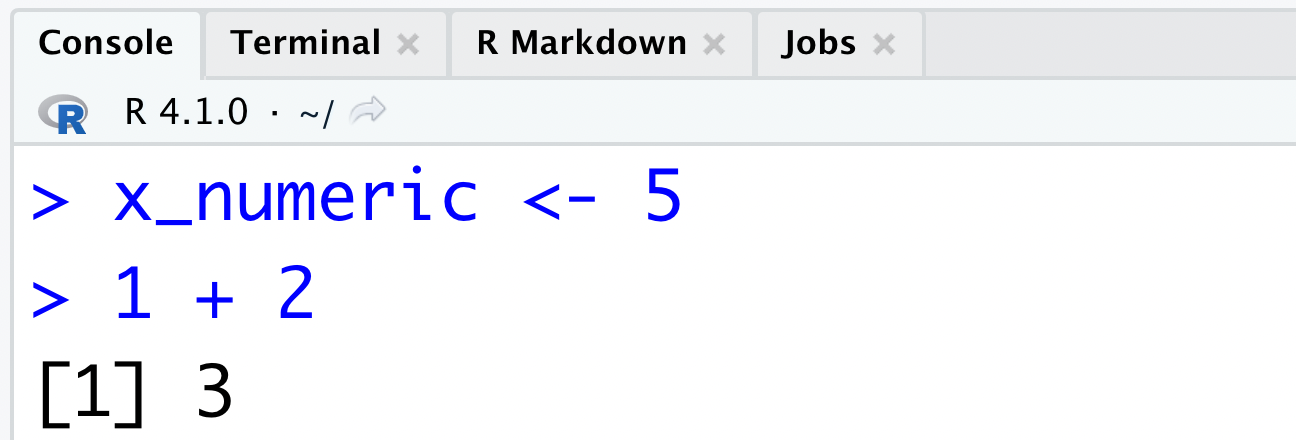
\includegraphics[width=0.7\linewidth]{pics/2noa} 

}

\caption{No output}\label{fig:noa}
\end{figure}

To verify it, you can run the code with just the object name to check its value. (For named objects, you can get their values by running codes with their object names.)

\begin{Shaded}
\begin{Highlighting}[]
\NormalTok{x\_numeric}
\CommentTok{\#\textgreater{} [1] 5}
\end{Highlighting}
\end{Shaded}

Great! You get the value 5, indicating that you have successfully assigned the value 5 to the name x\_numeric, and you have created a new object \texttt{x\_numeric}. You can use \texttt{x\_numeric} instead of \texttt{5} to do the subsequent calculations because \texttt{x\_numeric} and \texttt{5} have the same value.

You can also assign value(s) of any R expression (including operations and functions) to a name. Sometimes, the value(s) of an R expression may be unintuitive. To get the value(s) of an R expression, R will get the result of it firstly.

In this case, R will first calculate the result of \texttt{exp(3)\ /\ log(20,3)\ *\ 7} and assign the value of the result to a name. Let's see the following example.

\begin{Shaded}
\begin{Highlighting}[]
\NormalTok{y\_numeric }\OtherTok{\textless{}{-}} \FunctionTok{exp}\NormalTok{(}\DecValTok{3}\NormalTok{) }\SpecialCharTok{/} \FunctionTok{log}\NormalTok{(}\DecValTok{20}\NormalTok{,}\DecValTok{3}\NormalTok{) }\SpecialCharTok{*} \DecValTok{7}
\NormalTok{y\_numeric}
\CommentTok{\#\textgreater{} [1] 51.56119}
\end{Highlighting}
\end{Shaded}

Now you have successfully created an object \texttt{y\_numeric} with value 51.56119. Using the named object \texttt{y\_numeric}, you can do the same three calculations introduced at the beginning of this chapter as follows.

\begin{Shaded}
\begin{Highlighting}[]
\NormalTok{y\_numeric }\SpecialCharTok{+} \DecValTok{3}
\NormalTok{y\_numeric }\SpecialCharTok{{-}} \DecValTok{3}
\NormalTok{y\_numeric }\SpecialCharTok{/} \DecValTok{3}
\end{Highlighting}
\end{Shaded}

You can also try the following examples by yourself.

\begin{Shaded}
\begin{Highlighting}[]
\NormalTok{a }\OtherTok{\textless{}{-}} \FunctionTok{floor}\NormalTok{(}\DecValTok{7} \SpecialCharTok{/} \DecValTok{3}\NormalTok{) }
\NormalTok{a}
\NormalTok{b }\OtherTok{\textless{}{-}} \DecValTok{7}\SpecialCharTok{\%/\%}\DecValTok{3}
\NormalTok{b}
\end{Highlighting}
\end{Shaded}

Clearly, using the object assignment, we can greatly simplify our code and avoid redundancy.

Note that R object names are \textbf{case-sensitive}. For example, we have defined \texttt{x\_numeric}, but if you type \texttt{X\_numeric}, you will get an error message as follow.

\begin{Shaded}
\begin{Highlighting}[]
\NormalTok{X\_numeric}
\CommentTok{\#\textgreater{} Error in eval(expr, envir, enclos): object \textquotesingle{}X\_numeric\textquotesingle{} not found}
\end{Highlighting}
\end{Shaded}

\begin{infobox}{caution}

You can only use the names of named objects to get their values. If you type any unassigned name, e.g.~x0, you will see an error.

\begin{figure}

{\centering 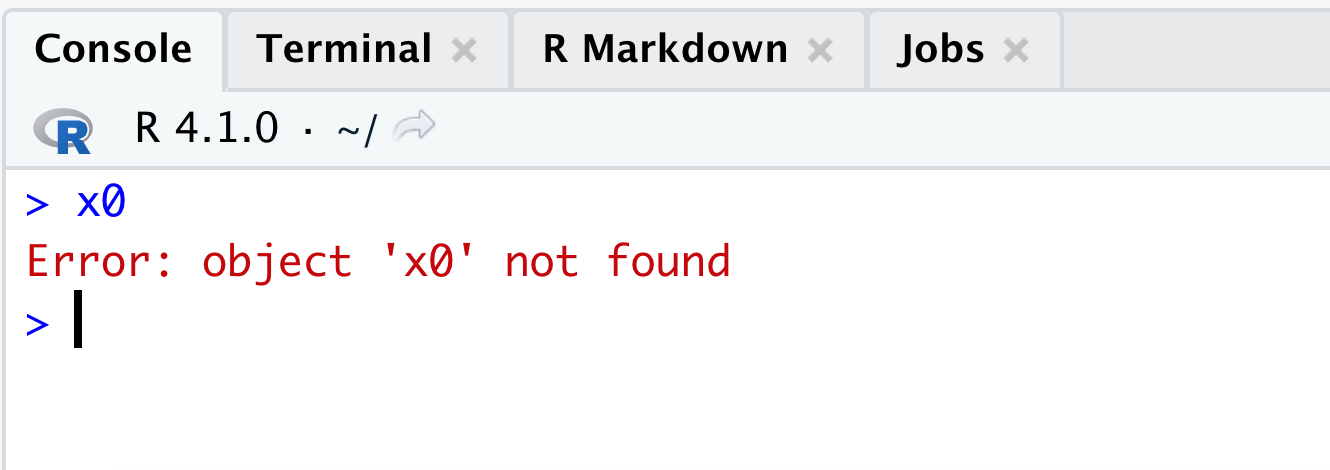
\includegraphics[width=0.8\linewidth]{pics/2object} 

}

\caption{x0 is not an object}\label{fig:obj}
\end{figure}

\end{infobox}

\hypertarget{review-objects-in-environment}{%
\subsection{Review objects in environment}\label{review-objects-in-environment}}

After creating new objects \texttt{x\_numeric} and \texttt{y\_numeric}, they will appear in the \textbf{Environment}, located in the top right panel (\textbf{panel3 in Figure \ref{fig:four}}). You can check all the \textbf{named objects} and their values in this area. It is helpful to monitor the environment from time to time to make sure everything look fine. Notice that objects without names will not be shown in the environment.

You can also see the list of all the named objects using function \texttt{ls()}.

\begin{Shaded}
\begin{Highlighting}[]
\FunctionTok{ls}\NormalTok{()}
\CommentTok{\#\textgreater{}  [1] "a"                                  "allx"                              }
\CommentTok{\#\textgreater{}  [3] "ally"                               "alpha1"                            }
\CommentTok{\#\textgreater{}  [5] "b"                                  "beta1"                             }
\CommentTok{\#\textgreater{}  [7] "Code"                               "cols"                              }
\CommentTok{\#\textgreater{}  [9] "d"                                  "data"                              }
\CommentTok{\#\textgreater{} [11] "date\_char"                          "ds16\_Nobel\_Laureates\_and\_Chocolate"}
\CommentTok{\#\textgreater{} [13] "Explanation"                        "frac"                              }
\CommentTok{\#\textgreater{} [15] "GaltonFamilies"                     "ind0"                              }
\CommentTok{\#\textgreater{} [17] "ind1"                               "lmod"                              }
\CommentTok{\#\textgreater{} [19] "logic1"                             "manilius"                          }
\CommentTok{\#\textgreater{} [21] "moon3"                              "my\_int"                            }
\CommentTok{\#\textgreater{} [23] "N"                                  "Name"                              }
\CommentTok{\#\textgreater{} [25] "Operation"                          "ori\_overall\_list"                  }
\CommentTok{\#\textgreater{} [27] "ori\_overall\_list\_logistic"          "ori\_overall\_list\_svm"              }
\CommentTok{\#\textgreater{} [29] "ori\_typeI\_list"                     "ori\_typeI\_list\_logistic"           }
\CommentTok{\#\textgreater{} [31] "ori\_typeI\_list\_svm"                 "ori\_typeII\_list"                   }
\CommentTok{\#\textgreater{} [33] "ori\_typeII\_list\_logistic"           "ori\_typeII\_list\_svm"               }
\CommentTok{\#\textgreater{} [35] "overall\_list"                       "overall\_list\_logistic"             }
\CommentTok{\#\textgreater{} [37] "overall\_list\_svm"                   "p1"                                }
\CommentTok{\#\textgreater{} [39] "p2"                                 "p3"                                }
\CommentTok{\#\textgreater{} [41] "Pattern"                            "pima"                              }
\CommentTok{\#\textgreater{} [43] "sheepstudio"                        "today"                             }
\CommentTok{\#\textgreater{} [45] "today\_char"                         "tr\_size0"                          }
\CommentTok{\#\textgreater{} [47] "tr\_size1"                           "typeI\_list"                        }
\CommentTok{\#\textgreater{} [49] "typeI\_list\_logistic"                "typeI\_list\_svm"                    }
\CommentTok{\#\textgreater{} [51] "typeII\_list"                        "typeII\_list\_logistic"              }
\CommentTok{\#\textgreater{} [53] "typeII\_list\_svm"                    "vec\_with\_name1"                    }
\CommentTok{\#\textgreater{} [55] "x"                                  "x\_numeric"                         }
\CommentTok{\#\textgreater{} [57] "x\_w\_name"                           "x\_wo\_name"                         }
\CommentTok{\#\textgreater{} [59] "x1"                                 "xs4"                               }
\CommentTok{\#\textgreater{} [61] "y"                                  "y\_numeric"                         }
\CommentTok{\#\textgreater{} [63] "y1"                                 "y2"                                }
\CommentTok{\#\textgreater{} [65] "y3"                                 "yb8"                               }
\CommentTok{\#\textgreater{} [67] "z1"}
\end{Highlighting}
\end{Shaded}

All the objects shown in the environment or the list have been saved in R, so they are available for future use directly. It is a good habit to do object assignments if you want to save important values for future use.

\hypertarget{Naming}{%
\subsection{Object naming rule}\label{Naming}}

Now you have created two named objects \texttt{x\_numeric} and \texttt{y\_numeric}. In general, R is very flexible in the name you give to an object,however, there are three important rules you need to follow.

\textbf{\emph{a. Must start with a letter or . (period)}}\\
If starting with period, the second character can't be a number.

\textbf{\emph{b. Can only contain letters, numbers, \texttt{\_} (underscore), and \texttt{.} (period)}}
One recommended naming style is to only use lowercase letters and numbers, and use underscore to separate words within a name. So you can use relatively longer names that is more readable.

\textbf{\emph{c.~Can not use special keywords as names.}}
For example, \texttt{TRUE\ \textless{}-\ 12} is not permitted as \texttt{TRUE} is a special keyword in R. You can see from the following that this assignment operation leads to an error message.

\begin{Shaded}
\begin{Highlighting}[]
\ConstantTok{TRUE} \OtherTok{\textless{}{-}} \DecValTok{12}
\CommentTok{\#\textgreater{} Error in TRUE \textless{}{-} 12: invalid (do\_set) left{-}hand side to assignment}
\end{Highlighting}
\end{Shaded}

Some commonly used reserved keywords that cannot be used as names are listed as below.

\begin{tabular}{l|l}
\hline
break & NA\\
\hline
else & NaN\\
\hline
FALSE & next\\
\hline
for & repeat\\
\hline
function & return\\
\hline
if & TRUE\\
\hline
Inf & while\\
\hline
\end{tabular}

To get a complete list of reserved words, you can run the following code.

\begin{Shaded}
\begin{Highlighting}[]
\NormalTok{?Reserved}
\end{Highlighting}
\end{Shaded}

\hypertarget{object-types}{%
\subsection{Object types}\label{object-types}}

In this section, you have learned about how to assign a value to a name. The values you assigned are all of numeric type. Actually, an object may contain more than one values. Also, the values it contains can be of other types than numeric, including character and logical. Depending on the \textbf{composition of values}, the object belongs to one particular type. We will focus on vectors in this chapter and discuss other object types in Chapter \ref{r-objects-other-types}.

\begin{tabular}{l|l}
\hline
Type & Section\\
\hline
Vector & \textbackslash{}@ref(vector)\\
\hline
Matrix & \textbackslash{}@ref(matrix)\\
\hline
Array & \textbackslash{}@ref(array)\\
\hline
Data Frame & \textbackslash{}@ref(dataframe)\\
\hline
List & \textbackslash{}@ref(list)\\
\hline
\end{tabular}

While some of the object types look more intuitive than others, you have nothing to worry about since we have this whole chapter and the next chapter devoted to the details of R objects. Objects are the building blocks of R programming and it will be time well spent mastering every object type.

\hypertarget{exercises-2}{%
\subsection{Exercises}\label{exercises-2}}

\begin{enumerate}
\def\labelenumi{\arabic{enumi}.}
\item
  Write R code to assign the value 20 to the name \texttt{num\_1}.
\item
  Which of the following is a valid object name in R?
\end{enumerate}

\begin{itemize}
\tightlist
\item
  \texttt{2.True}
\item
  \texttt{else}
\item
  \texttt{I\_am\_not\_a\_valid\_name}
\item
  \texttt{I\_am\_a\_Pretty\#\_name}
\end{itemize}

\begin{enumerate}
\def\labelenumi{\arabic{enumi}.}
\setcounter{enumi}{2}
\tightlist
\item
  Write R code to get the list of all objects in the environment.
\end{enumerate}

\hypertarget{vector}{%
\section{Vectors: Numeric, Character, and Logical}\label{vector}}

In the last section, you have had a basic understanding of R objects and how to do object assignments. From this section, we will start to introduce different types of R objects one by one. The first R object type we want to introduce is called vector. \textbf{Vector} is the simplest object type in R, which contains one or more values of the \textbf{same type}. We will introduce numeric vector, character vector, and logical vector in this section. Let's begin with numeric vector.

\hypertarget{numeric-vector}{%
\subsection{Numeric vector}\label{numeric-vector}}

\textbf{\emph{a. Create numeric vectors}}

A \textbf{numeric vector} is a type of vector that only contains values of numeric type. For example, \texttt{6} is a numeric vector with one element of value 6. For vectors, the number of elements corresponds to the length of vector, so \texttt{6} is a numeric vector with length 1.

After assigning the value 6 to the name x1, you have created a new vector \texttt{x1} with the same value as \texttt{6}, so \texttt{x1} is also a numeric vector. And you can refer to \texttt{x1} in the subsequent calculations.

\begin{Shaded}
\begin{Highlighting}[]
\DecValTok{6}                         \CommentTok{\#a numeric vector with length 1}
\NormalTok{x1 }\OtherTok{\textless{}{-}} \DecValTok{6}                   \CommentTok{\#x1 is also a numeric vector with length 1}
\NormalTok{x1                        }\CommentTok{\#check the value of x1}
\end{Highlighting}
\end{Shaded}

But can a numeric vector contain more than one values? The answer is a big YES! In R, you can use the \texttt{c()} function (\texttt{c} is short for combine) to combine elements into a numeric vector.

\begin{Shaded}
\begin{Highlighting}[]
\FunctionTok{c}\NormalTok{(}\DecValTok{1}\NormalTok{, }\DecValTok{3}\NormalTok{, }\DecValTok{3}\NormalTok{, }\DecValTok{5}\NormalTok{, }\DecValTok{5}\NormalTok{)          }\CommentTok{\#use c() to combine elements into a numeric vector of length 5}
\NormalTok{y1 }\OtherTok{\textless{}{-}} \FunctionTok{c}\NormalTok{(}\DecValTok{1}\NormalTok{, }\DecValTok{3}\NormalTok{, }\DecValTok{3}\NormalTok{, }\DecValTok{5}\NormalTok{, }\DecValTok{5}\NormalTok{)    }\CommentTok{\#y1 is also a numeric vector of length 5}
\NormalTok{y1                        }\CommentTok{\#check the value of y1}
\FunctionTok{length}\NormalTok{(y1)                }\CommentTok{\#length of a vector}
\end{Highlighting}
\end{Shaded}

In this example, you have created a length-5 object using the \texttt{c()} function with arguments containing the five elements separated by comma. Since the value of each element is a number, the object is a numeric vector.

If you assign the values to the name y1, you will get a new numeric vector \texttt{y1} with 5 values. Notice that the second and third elements have the same value 3 in \texttt{y1}. You can verify the contents of \texttt{y1} and check the length of it through the \texttt{length()} function.

\begin{infobox}{caution}
When you assign several values to a name, the order of the values will not change after assignment. If you create two numeric vectors with same numbers of different orders, these objects will have different values. For example,

\begin{Shaded}
\begin{Highlighting}[]
\NormalTok{y2 }\OtherTok{\textless{}{-}} \FunctionTok{c}\NormalTok{(}\DecValTok{1}\NormalTok{, }\DecValTok{3}\NormalTok{, }\DecValTok{5}\NormalTok{, }\DecValTok{7}\NormalTok{, }\DecValTok{9}\NormalTok{)    }
\NormalTok{y2                        }
\NormalTok{y3 }\OtherTok{\textless{}{-}} \FunctionTok{c}\NormalTok{(}\DecValTok{9}\NormalTok{, }\DecValTok{7}\NormalTok{, }\DecValTok{5}\NormalTok{, }\DecValTok{3}\NormalTok{, }\DecValTok{1}\NormalTok{)    }
\NormalTok{y3}
\end{Highlighting}
\end{Shaded}

Here, \texttt{y2} and \texttt{y3} have different values.

\end{infobox}

If you include several numeric vectors in \texttt{c()}, you will also create a numeric vector as a combination of the input numeric vectors. For example, you can create a numeric vector with values from two numeric vectors. Of course you can create a new numeric vector \texttt{z1} using object assignment.

\begin{Shaded}
\begin{Highlighting}[]
\FunctionTok{c}\NormalTok{(}\FunctionTok{c}\NormalTok{(}\DecValTok{1}\NormalTok{,}\DecValTok{2}\NormalTok{), }\FunctionTok{c}\NormalTok{(}\DecValTok{3}\NormalTok{,}\DecValTok{4}\NormalTok{))          }\CommentTok{\#use c() to combine several numeric vectors into one numeric vector}
\NormalTok{z1 }\OtherTok{\textless{}{-}} \FunctionTok{c}\NormalTok{(}\FunctionTok{c}\NormalTok{(}\DecValTok{1}\NormalTok{,}\DecValTok{2}\NormalTok{), }\FunctionTok{c}\NormalTok{(}\DecValTok{3}\NormalTok{,}\DecValTok{4}\NormalTok{))}
\NormalTok{z1}
\FunctionTok{length}\NormalTok{(z1)}
\end{Highlighting}
\end{Shaded}

After creating vectors, you can use the function \texttt{class()} to check its \textbf{class}.

\begin{Shaded}
\begin{Highlighting}[]
\FunctionTok{class}\NormalTok{(x1)}
\CommentTok{\#\textgreater{} [1] "numeric"}
\FunctionTok{class}\NormalTok{(y1)}
\CommentTok{\#\textgreater{} [1] "numeric"}
\FunctionTok{class}\NormalTok{(z1)}
\CommentTok{\#\textgreater{} [1] "numeric"}
\end{Highlighting}
\end{Shaded}

From the results, you will know that \texttt{x1}, \texttt{y1} and \texttt{z1} are numeric, which is the reason why they are called \emph{numeric vectors}.

\textbf{\emph{b. Operations between two numeric vectors}}

Since numeric vectors are made of numbers, you can do \textbf{arithmetic operations} between them, just like the fancy calculator in Section \ref{Calculator}. If two vectors are of the \textbf{same length}, the calculation is done \textbf{elementwisely}. In other words, R will perform the operation separately for each element. First, let's create another vector \texttt{x2} of length 1 and do addition with \texttt{x1}.

\begin{Shaded}
\begin{Highlighting}[]
\NormalTok{x2 }\OtherTok{\textless{}{-}} \DecValTok{3}
\NormalTok{x1 }\SpecialCharTok{+}\NormalTok{ x2}
\CommentTok{\#\textgreater{} [1] 9}
\end{Highlighting}
\end{Shaded}

Then obviously you will get 9!

Similarly, you can create another vector \texttt{y2} of the same length as vector \texttt{y1}. Then, you can do operations between \texttt{y1} and \texttt{y2}.

\begin{Shaded}
\begin{Highlighting}[]
\NormalTok{y2 }\OtherTok{\textless{}{-}} \FunctionTok{c}\NormalTok{(}\DecValTok{2}\NormalTok{, }\DecValTok{4}\NormalTok{, }\DecValTok{1}\NormalTok{, }\DecValTok{3}\NormalTok{, }\DecValTok{2}\NormalTok{)}
\NormalTok{y1 }\SpecialCharTok{+}\NormalTok{ y2}
\CommentTok{\#\textgreater{} [1] 3 7 4 8 7}
\end{Highlighting}
\end{Shaded}

The result is yet another length-5 vector. To check the calculation was indeed done elementwisely, you can verify that the value of the first element is \(1 + 2 = 3\), and value of the second element is \(3 + 4 = 7\), etc.

Since the calculation is done elementwisely, people normally would want the two vectors to have the same length. However, there is a \textbf{recycling} rule in R, which is sometimes quite useful and enables us to write simpler code. Specifically, if one vector is shorter than the other vector, R will recycle (repeat) the shorter vector until it matches in length with the longer one. This recycling is particularly helpful for an operator between a \textbf{length\textgreater1} vector and a \textbf{length-1} vector. Let's see an example.

\begin{Shaded}
\begin{Highlighting}[]
\NormalTok{y1 }\SpecialCharTok{+}\NormalTok{ x1}
\CommentTok{\#\textgreater{} [1]  7  9  9 11 11}
\end{Highlighting}
\end{Shaded}

From the result, you can see that each element in \texttt{y1} is added by 6.

The followings are a few additional examples you can try.

\begin{Shaded}
\begin{Highlighting}[]
\NormalTok{y1 }\SpecialCharTok{*}\NormalTok{ x2}
\NormalTok{y1 }\SpecialCharTok{/} \DecValTok{5}
\NormalTok{y2 }\SpecialCharTok{{-}}\NormalTok{ x1}
\end{Highlighting}
\end{Shaded}

\hypertarget{vector-character}{%
\subsection{Character vector}\label{vector-character}}

\textbf{\emph{a. Create character vectors}}

Now, let's move to character vectors. In a \textbf{character vector}, the value of each element is of character type, which means each value is a \textbf{string}. A \textbf{string} is a sequence of characters (including letters, numbers, or symbols) surrounded by a pair of double quotes (\texttt{""}) or single quotes (\texttt{\textquotesingle{}\textquotesingle{}}). To be consistent, we will stick with double quotes in this book.

Let's first create a character vector \texttt{sheepstudio} which only has one element. You can then check the value of this vector by typing its name and verify the vector type by using \texttt{class()}.

\begin{Shaded}
\begin{Highlighting}[]
\NormalTok{sheepstudio }\OtherTok{\textless{}{-}} \StringTok{"sheep@007"} 
\NormalTok{sheepstudio}
\FunctionTok{class}\NormalTok{(sheepstudio)}
\end{Highlighting}
\end{Shaded}

\begin{infobox}{caution}

Double quotes need to be paired in strings. If you miss the right double quote, R will show a plus on the next line, waiting for you to finish the command. If this happens, you can either enter the matching double quote, or press ESC to escape this command.

\begin{figure}

{\centering 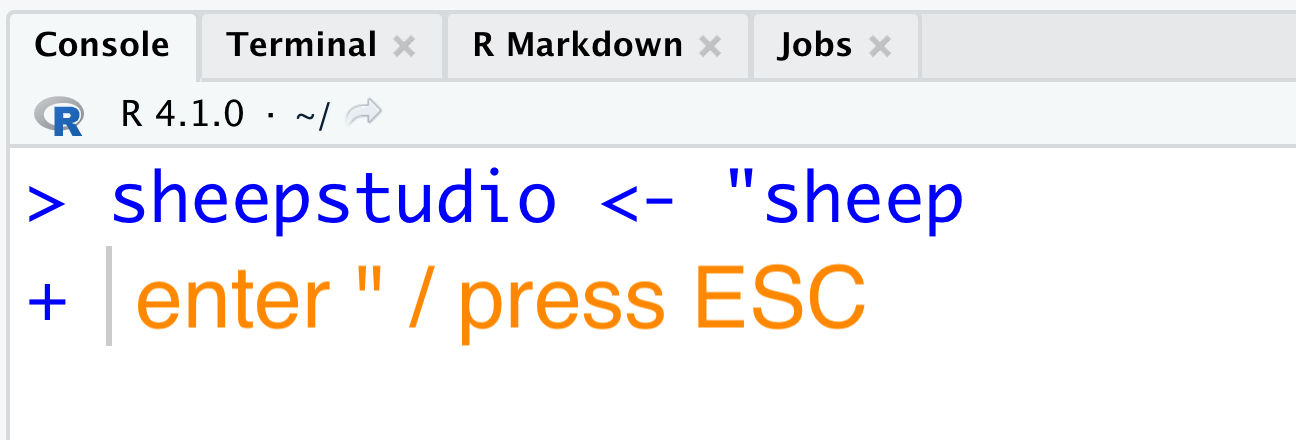
\includegraphics[width=0.7\linewidth]{pics/2quo} 

}

\caption{Miss the right quotation mark}\label{fig:quo}
\end{figure}

\end{infobox}

Similar to a numeric vector, you can use the \texttt{c()} function to combine several strings to create a character vector. You can verify the number of strings in the character vector by using \texttt{length()}, and \texttt{nchar()} can help you get the number of characters in each string.

\begin{Shaded}
\begin{Highlighting}[]
\NormalTok{animals }\OtherTok{\textless{}{-}} \FunctionTok{c}\NormalTok{(}\StringTok{"sheep@29"}\NormalTok{, }\StringTok{"pig$29"}\NormalTok{, }\StringTok{"monkey"}\NormalTok{)}
\NormalTok{animals}
\FunctionTok{length}\NormalTok{(animals)}
\FunctionTok{nchar}\NormalTok{(animals)}
\end{Highlighting}
\end{Shaded}

Note that if you have a vector consisted of numbers with surrounding double quotes, it is also a character vector. (``4'' and ``29'' are strings)

\begin{Shaded}
\begin{Highlighting}[]
\NormalTok{num\_vec }\OtherTok{\textless{}{-}} \FunctionTok{c}\NormalTok{(}\DecValTok{4}\NormalTok{, }\DecValTok{29}\NormalTok{)}
\NormalTok{char\_vec }\OtherTok{\textless{}{-}} \FunctionTok{c}\NormalTok{(}\StringTok{"4"}\NormalTok{, }\StringTok{"29"}\NormalTok{) }
\FunctionTok{class}\NormalTok{(num\_vec)}
\CommentTok{\#\textgreater{} [1] "numeric"}
\FunctionTok{class}\NormalTok{(char\_vec)}
\CommentTok{\#\textgreater{} [1] "character"}
\end{Highlighting}
\end{Shaded}

\textbf{\emph{b. Concatenate several strings into a single string}}

Next, we will introduce how to concatenate several strings into a single string. To do this, you can use the \texttt{paste()} function. First, let's create a character vector with four elements,

\begin{Shaded}
\begin{Highlighting}[]
\NormalTok{four\_strings }\OtherTok{\textless{}{-}} \FunctionTok{c}\NormalTok{(}\StringTok{"This"}\NormalTok{, }\StringTok{"is"}\NormalTok{, }\StringTok{"Sheep@29"}\NormalTok{, }\StringTok{"$Studio"}\NormalTok{)}
\FunctionTok{length}\NormalTok{(four\_strings) }\CommentTok{\#verify the number of strings}
\end{Highlighting}
\end{Shaded}

Then use \texttt{paste()} instead of \texttt{c()},

\begin{Shaded}
\begin{Highlighting}[]
\NormalTok{one\_long\_string }\OtherTok{\textless{}{-}} \FunctionTok{paste}\NormalTok{(}\StringTok{"This"}\NormalTok{, }\StringTok{"is"}\NormalTok{, }\StringTok{"Sheep@29"}\NormalTok{, }\StringTok{"$Studio"}\NormalTok{)}
\NormalTok{one\_long\_string}
\CommentTok{\#\textgreater{} [1] "This is Sheep@29 $Studio"}
\end{Highlighting}
\end{Shaded}

\begin{Shaded}
\begin{Highlighting}[]
\FunctionTok{class}\NormalTok{(one\_long\_string)}
\FunctionTok{length}\NormalTok{(one\_long\_string) }\CommentTok{\#verify the number of strings}
\end{Highlighting}
\end{Shaded}

From the results, you can see that \texttt{one\_long\_string} is a character vector with length 1, and the value of \texttt{one\_long\_string} is a single string with space between the individual strings.

You may notice that in \texttt{paste()}, the default separator between the individual strings is space. Actually you can change the separator by setting the \texttt{sep} argument in \texttt{paste()}. For example, you can separate the individual strings with comma,

\begin{Shaded}
\begin{Highlighting}[]
\NormalTok{comma }\OtherTok{\textless{}{-}} \FunctionTok{paste}\NormalTok{(}\StringTok{"This"}\NormalTok{, }\StringTok{"is"}\NormalTok{, }\StringTok{"Sheep@29"}\NormalTok{, }\StringTok{"$Studio"}\NormalTok{, }\AttributeTok{sep =} \StringTok{","}\NormalTok{) }
\NormalTok{comma}
\CommentTok{\#\textgreater{} [1] "This,is,Sheep@29,$Studio"}
\end{Highlighting}
\end{Shaded}

If you don't want to use a separator, you can use the \texttt{paste0()} function.

\begin{Shaded}
\begin{Highlighting}[]
\NormalTok{nosep }\OtherTok{\textless{}{-}} \FunctionTok{paste0}\NormalTok{(}\StringTok{"This"}\NormalTok{, }\StringTok{"is"}\NormalTok{, }\StringTok{"Sheep@29"}\NormalTok{, }\StringTok{"$Studio"}\NormalTok{) }
\NormalTok{nosep}
\CommentTok{\#\textgreater{} [1] "ThisisSheep@29$Studio"}
\end{Highlighting}
\end{Shaded}

If you would like to concatenate the strings of a vector into a longer string, you need to specify the \texttt{collapse} argument as the separator instead of \texttt{sep} in the \texttt{paste()} function.

\begin{Shaded}
\begin{Highlighting}[]
\FunctionTok{paste}\NormalTok{(four\_strings, }\AttributeTok{collapse =} \StringTok{""}\NormalTok{)}
\CommentTok{\#\textgreater{} [1] "ThisisSheep@29$Studio"}
\FunctionTok{paste}\NormalTok{(four\_strings, }\AttributeTok{collapse =} \StringTok{","}\NormalTok{)}
\CommentTok{\#\textgreater{} [1] "This,is,Sheep@29,$Studio"}
\FunctionTok{paste}\NormalTok{(four\_strings)                 }\DocumentationTok{\#\#doesn\textquotesingle{}t work without the collapse argument}
\CommentTok{\#\textgreater{} [1] "This"     "is"       "Sheep@29" "$Studio"}
\end{Highlighting}
\end{Shaded}

In addition to paste several strings into one long string, you can also use the \texttt{paste()} function paste two character vectors, where the pair of strings will be pasted elementwisely.

\begin{Shaded}
\begin{Highlighting}[]
\NormalTok{Month\_vec }\OtherTok{\textless{}{-}} \FunctionTok{c}\NormalTok{(}\StringTok{"July"}\NormalTok{, }\StringTok{"August"}\NormalTok{)}
\NormalTok{Year\_vec }\OtherTok{\textless{}{-}} \FunctionTok{c}\NormalTok{(}\StringTok{"2007"}\NormalTok{, }\StringTok{"2008"}\NormalTok{)}
\FunctionTok{paste}\NormalTok{(Month\_vec, Year\_vec)}
\CommentTok{\#\textgreater{} [1] "July 2007"   "August 2008"}
\end{Highlighting}
\end{Shaded}

\textbf{\emph{c.~Change case}}

In character vectors, each string can contain both uppercase and lowercase letters. You can unify the cases of all letters inside a vector. Let's review the character vector \texttt{four\_strings} at first,

\begin{Shaded}
\begin{Highlighting}[]
\NormalTok{four\_strings }\OtherTok{\textless{}{-}} \FunctionTok{c}\NormalTok{(}\StringTok{"This"}\NormalTok{, }\StringTok{"is"}\NormalTok{, }\StringTok{"Sheep@29"}\NormalTok{, }\StringTok{"$Studio"}\NormalTok{)}
\NormalTok{four\_strings}
\CommentTok{\#\textgreater{} [1] "This"     "is"       "Sheep@29" "$Studio"}
\end{Highlighting}
\end{Shaded}

Then use the \texttt{tolower()} function to convert all letters to lower case,

\begin{Shaded}
\begin{Highlighting}[]
\FunctionTok{tolower}\NormalTok{(four\_strings)}
\CommentTok{\#\textgreater{} [1] "this"     "is"       "sheep@29" "$studio"}
\end{Highlighting}
\end{Shaded}

The opposite function of \texttt{tolower()} is \texttt{toupper()}, which converts all letters to upper case,

\begin{Shaded}
\begin{Highlighting}[]
\FunctionTok{toupper}\NormalTok{(four\_strings)}
\CommentTok{\#\textgreater{} [1] "THIS"     "IS"       "SHEEP@29" "$STUDIO"}
\end{Highlighting}
\end{Shaded}

\hypertarget{logical-vector}{%
\subsection{Logical vector}\label{logical-vector}}

So far we have created several numeric vectors and character vectors. Some vectors have names, and some do not. You can see all the \textbf{named objects} by using the \texttt{ls()} function.

\begin{Shaded}
\begin{Highlighting}[]
\FunctionTok{ls}\NormalTok{()}
\CommentTok{\#\textgreater{}  [1] "a"                                  "allx"                              }
\CommentTok{\#\textgreater{}  [3] "ally"                               "alpha1"                            }
\CommentTok{\#\textgreater{}  [5] "animals"                            "b"                                 }
\CommentTok{\#\textgreater{}  [7] "beta1"                              "char\_vec"                          }
\CommentTok{\#\textgreater{}  [9] "Code"                               "cols"                              }
\CommentTok{\#\textgreater{} [11] "comma"                              "d"                                 }
\CommentTok{\#\textgreater{} [13] "data"                               "date\_char"                         }
\CommentTok{\#\textgreater{} [15] "ds16\_Nobel\_Laureates\_and\_Chocolate" "Explanation"                       }
\CommentTok{\#\textgreater{} [17] "four\_strings"                       "frac"                              }
\CommentTok{\#\textgreater{} [19] "GaltonFamilies"                     "ind0"                              }
\CommentTok{\#\textgreater{} [21] "ind1"                               "key\_mat"                           }
\CommentTok{\#\textgreater{} [23] "Keys"                               "lmod"                              }
\CommentTok{\#\textgreater{} [25] "logic1"                             "manilius"                          }
\CommentTok{\#\textgreater{} [27] "Month\_vec"                          "moon3"                             }
\CommentTok{\#\textgreater{} [29] "my\_int"                             "N"                                 }
\CommentTok{\#\textgreater{} [31] "Name"                               "nosep"                             }
\CommentTok{\#\textgreater{} [33] "num\_vec"                            "one\_long\_string"                   }
\CommentTok{\#\textgreater{} [35] "Operation"                          "ori\_overall\_list"                  }
\CommentTok{\#\textgreater{} [37] "ori\_overall\_list\_logistic"          "ori\_overall\_list\_svm"              }
\CommentTok{\#\textgreater{} [39] "ori\_typeI\_list"                     "ori\_typeI\_list\_logistic"           }
\CommentTok{\#\textgreater{} [41] "ori\_typeI\_list\_svm"                 "ori\_typeII\_list"                   }
\CommentTok{\#\textgreater{} [43] "ori\_typeII\_list\_logistic"           "ori\_typeII\_list\_svm"               }
\CommentTok{\#\textgreater{} [45] "overall\_list"                       "overall\_list\_logistic"             }
\CommentTok{\#\textgreater{} [47] "overall\_list\_svm"                   "p1"                                }
\CommentTok{\#\textgreater{} [49] "p2"                                 "p3"                                }
\CommentTok{\#\textgreater{} [51] "Pattern"                            "pima"                              }
\CommentTok{\#\textgreater{} [53] "Section"                            "sheepstudio"                       }
\CommentTok{\#\textgreater{} [55] "today"                              "today\_char"                        }
\CommentTok{\#\textgreater{} [57] "tr\_size0"                           "tr\_size1"                          }
\CommentTok{\#\textgreater{} [59] "Type"                               "typeI\_list"                        }
\CommentTok{\#\textgreater{} [61] "typeI\_list\_logistic"                "typeI\_list\_svm"                    }
\CommentTok{\#\textgreater{} [63] "typeII\_list"                        "typeII\_list\_logistic"              }
\CommentTok{\#\textgreater{} [65] "typeII\_list\_svm"                    "vec\_with\_name1"                    }
\CommentTok{\#\textgreater{} [67] "x"                                  "x\_numeric"                         }
\CommentTok{\#\textgreater{} [69] "x\_w\_name"                           "x\_wo\_name"                         }
\CommentTok{\#\textgreater{} [71] "x1"                                 "x2"                                }
\CommentTok{\#\textgreater{} [73] "xs4"                                "y"                                 }
\CommentTok{\#\textgreater{} [75] "y\_numeric"                          "y1"                                }
\CommentTok{\#\textgreater{} [77] "y2"                                 "y3"                                }
\CommentTok{\#\textgreater{} [79] "yb8"                                "Year\_vec"                          }
\CommentTok{\#\textgreater{} [81] "z1"}
\end{Highlighting}
\end{Shaded}

As introduced in Section \ref{Object-Assignment}, another way to check the named objects is via the environment panel as shown in Figure \ref{fig:enviro}.

\begin{figure}

{\centering 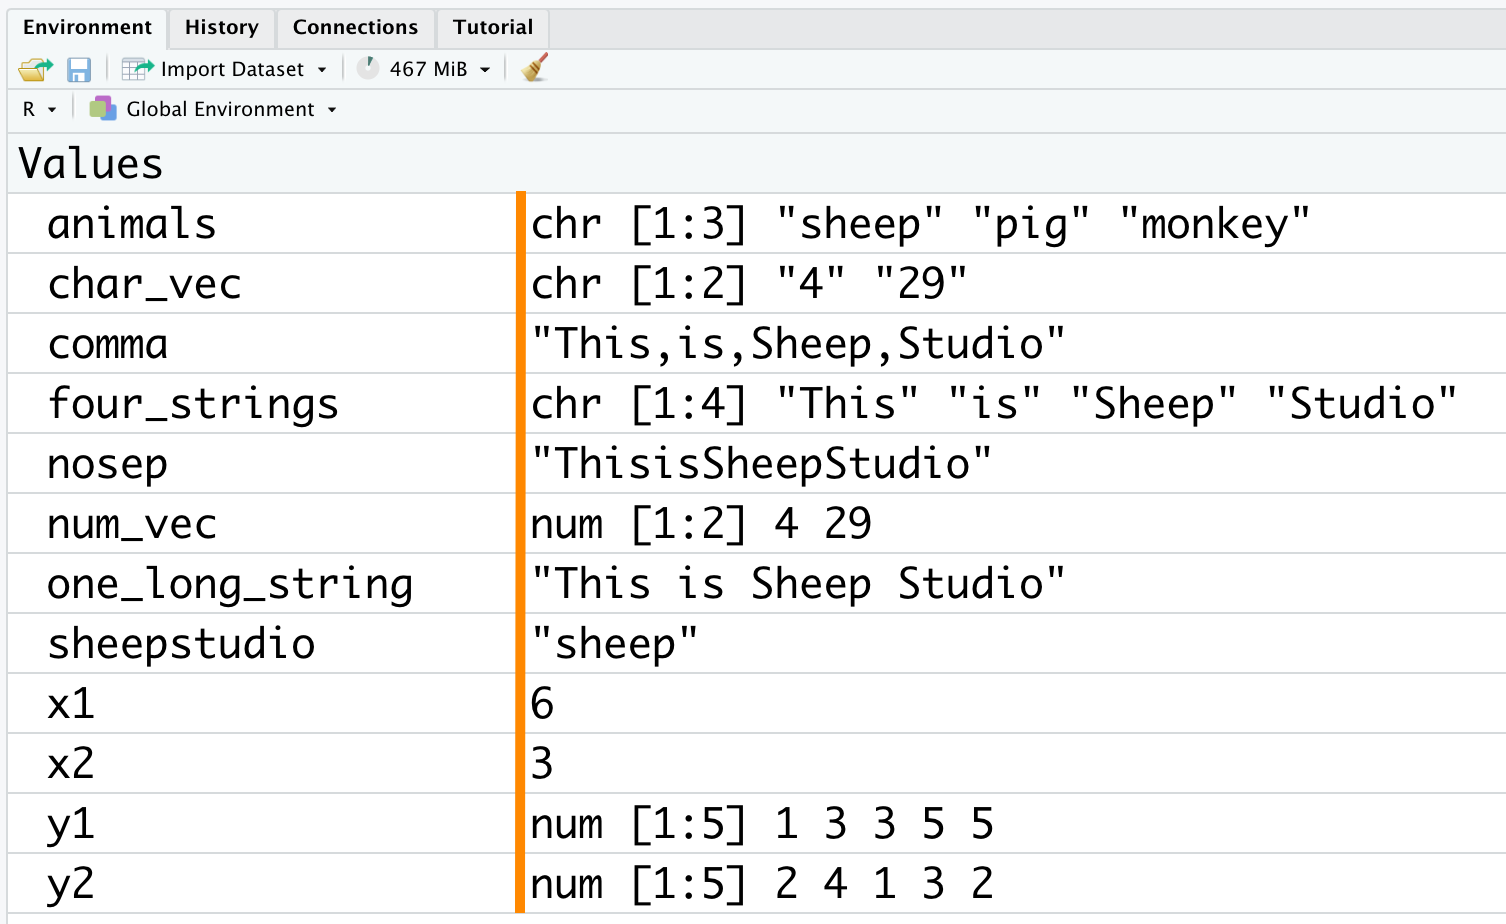
\includegraphics[width=0.7\linewidth]{pics/2enviro} 

}

\caption{Environment}\label{fig:enviro}
\end{figure}

We can see that the environment panel has two columns, with the first column showing the list of object names, and the second column showing the corresponding information for each object. The information includes the vector type (\emph{chr} is short for character and \emph{num} is short for numeric), the vector length, and the first few values of the vector. Note that if the vector is of length 1 (for example \texttt{x1}), the environment will not show the type or the length.

\begin{infobox}{caution}
By now you have created several objects, and you will find that the objects will not be saved in R if you don't assign their values to names, for example, the results of \texttt{x1\ +\ x2} and \texttt{y1\ +\ y2} are not shown in the environment.

\end{infobox}

Before introducing the \emph{logical vector}, let's first learn a function called \texttt{is.numeric()}, which checks whether a vector is of numeric type,

\begin{Shaded}
\begin{Highlighting}[]
\FunctionTok{is.numeric}\NormalTok{(y1) }\CommentTok{\#Is y1 of numeric type?}
\CommentTok{\#\textgreater{} [1] TRUE}
\end{Highlighting}
\end{Shaded}

Similar to \texttt{is.numeric()}, you can also use \texttt{is.character()} function to check if the given vector is of character type.

\begin{Shaded}
\begin{Highlighting}[]
\FunctionTok{is.character}\NormalTok{(y1) }\CommentTok{\#Is y1 of character type?}
\CommentTok{\#\textgreater{} [1] FALSE}
\end{Highlighting}
\end{Shaded}

You may notice that results are \texttt{TRUE} or \texttt{FALSE} from the above codes. Actually, \textbf{logical vectors} are vectors that only use \texttt{TRUE} or \texttt{FALSE} as values. Note that \texttt{TRUE} and \texttt{FALSE} are logical constants in R. Similarly, you can use \texttt{is.logical()} to check if the vector is of logical type, or you can use \texttt{class()} to find out the exact type.

\begin{Shaded}
\begin{Highlighting}[]
\NormalTok{logic1 }\OtherTok{\textless{}{-}} \FunctionTok{c}\NormalTok{(}\ConstantTok{TRUE}\NormalTok{, }\ConstantTok{FALSE}\NormalTok{, }\ConstantTok{TRUE}\NormalTok{) }\CommentTok{\#you can also use the c() function to create a logical vector}
\FunctionTok{is.logical}\NormalTok{(logic1)}
\FunctionTok{class}\NormalTok{(logic1)}
\end{Highlighting}
\end{Shaded}

You can also use \texttt{T} to represent \texttt{TRUE} and \texttt{F} to represent \texttt{FALSE} in logical vectors.

\begin{Shaded}
\begin{Highlighting}[]
\NormalTok{logic2 }\OtherTok{\textless{}{-}} \FunctionTok{c}\NormalTok{(T, F, F)}
\FunctionTok{is.logical}\NormalTok{(logic2)}
\FunctionTok{class}\NormalTok{(logic2)}
\end{Highlighting}
\end{Shaded}

It is worth to point out that you don't want to put a pair of double quotes around \texttt{TRUE} or \texttt{FALSE} when you use them as logical values. If you do that, a character vector will be generated instead.

\begin{Shaded}
\begin{Highlighting}[]
\NormalTok{char }\OtherTok{\textless{}{-}} \FunctionTok{c}\NormalTok{(}\StringTok{"TRUE"}\NormalTok{, }\StringTok{"FALSE"}\NormalTok{, }\StringTok{"TRUE"}\NormalTok{)}
\FunctionTok{is.logical}\NormalTok{(char)}
\FunctionTok{class}\NormalTok{(char)}
\end{Highlighting}
\end{Shaded}

Note that the keywords \texttt{TRUE} and \texttt{FALSE} are case sensitive, and all letters inside them need to be in \textbf{upper case}. If you change any letter to the lower case, you will get an error, because \texttt{True} is neither a logical constant nor a defined object.

\begin{Shaded}
\begin{Highlighting}[]
\NormalTok{tlogic }\OtherTok{\textless{}{-}}\NormalTok{ True}
\CommentTok{\#\textgreater{} Error in eval(expr, envir, enclos): object \textquotesingle{}True\textquotesingle{} not found}
\end{Highlighting}
\end{Shaded}

\hypertarget{exercises-3}{%
\subsection{Exercises}\label{exercises-3}}

\begin{enumerate}
\def\labelenumi{\arabic{enumi}.}
\item
  Write R code to create a numeric vector named \texttt{vec\_1} with values \texttt{7\ 24\ 8\ \ 26}, get its length, and find out its type.
\item
  Write R code to create a character vector named \texttt{char\_1} with values \texttt{"I"}, \texttt{"am"}, \texttt{"learning"}, \texttt{"R!"}, get its length, find out its type, and concatenate the vector into a single string with space as the separator.
\item
  For the \texttt{char\_1} defined in Q2, find the number of characters in each string, and convert each string to upper case.
\item
  Create a length-2 logical vector representing whether \texttt{vec\_1} and \texttt{char\_1} are of character type.
\end{enumerate}

\hypertarget{attr-coercion}{%
\section{Vectors: Attributes and Coercion}\label{attr-coercion}}

Having learned vectors in Section \ref{vector}, we first introduce two commonly used numeric classes (integers and doubles), then introduce the concept of \textbf{attributes} from a \textbf{named vector}, and discuss the \textbf{coercion} rule when you combine values of different types into a single vector.

\hypertarget{integer-double}{%
\subsection{Integers and Doubles}\label{integer-double}}

The two most commonly used numeric classes in R are \textbf{integers} and \textbf{doubles}. As the names suggest, a vector of integers contain integers, and a vector of double class contain double precision numeric values. One obvious benefit of integers over doubles is the significant save of memory.

To create an integer vector, you can still use the \texttt{c()} function with the integers separated by comma as arguments. However, you need to put an ``L'' after each integer. Let's create an integer and check its \texttt{class()}. As a contrast, we also create a vector without the ``L''s.

\begin{Shaded}
\begin{Highlighting}[]
\NormalTok{my\_int }\OtherTok{\textless{}{-}} \FunctionTok{c}\NormalTok{(1L, 3L, 4L)}
\FunctionTok{class}\NormalTok{(my\_int)}
\CommentTok{\#\textgreater{} [1] "integer"}
\NormalTok{my\_double }\OtherTok{\textless{}{-}} \FunctionTok{c}\NormalTok{(}\DecValTok{1}\NormalTok{, }\DecValTok{3}\NormalTok{, }\DecValTok{4}\NormalTok{)}
\FunctionTok{class}\NormalTok{(my\_double)}
\CommentTok{\#\textgreater{} [1] "numeric"}
\end{Highlighting}
\end{Shaded}

In addition to \texttt{class()}, another useful function \texttt{typeof()} gives us the \textbf{internal storage type} of an R object, which tells how the information is stored. And the function \texttt{str()} gives the detailed \textbf{structure} of an R object along with the first few values.

Whenever we have an R object, it is useful to apply \texttt{class()}, \texttt{typeof()}, and \texttt{str()} on it.

\begin{Shaded}
\begin{Highlighting}[]
\FunctionTok{typeof}\NormalTok{(my\_int)}
\CommentTok{\#\textgreater{} [1] "integer"}
\FunctionTok{typeof}\NormalTok{(my\_double) }
\CommentTok{\#\textgreater{} [1] "double"}
\FunctionTok{str}\NormalTok{(my\_int)}
\CommentTok{\#\textgreater{}  int [1:3] 1 3 4}
\FunctionTok{str}\NormalTok{(my\_double)}
\CommentTok{\#\textgreater{}  num [1:3] 1 3 4}
\end{Highlighting}
\end{Shaded}

From the \texttt{typeof()} and \texttt{str()} results, \texttt{my\_int} is stored as integers while \texttt{my\_double} is stored as double precision numeric values. Note that although the object \texttt{my\_double} looks to be an integer, it is stored as a double precision object.

\begin{infobox}{caution}
Despite the differences between integers and doubles, you can usually ignore their differences unless you are working on a very big data set. R will automatically convert objects between integers and doubles when necessary.

\end{infobox}

Another vector classes in R is \textbf{complex}, which stores complex numbers.

\begin{Shaded}
\begin{Highlighting}[]
\NormalTok{my\_complex }\OtherTok{\textless{}{-}} \FunctionTok{c}\NormalTok{(}\DecValTok{1} \SpecialCharTok{+}\NormalTok{ 2i, }\DecValTok{3} \SpecialCharTok{+}\NormalTok{ 4i, }\SpecialCharTok{{-}}\DecValTok{3} \SpecialCharTok{{-}}\NormalTok{ 4i)}
\NormalTok{my\_complex}
\CommentTok{\#\textgreater{} [1]  1+2i  3+4i {-}3{-}4i}
\FunctionTok{class}\NormalTok{(my\_complex)}
\CommentTok{\#\textgreater{} [1] "complex"}
\FunctionTok{typeof}\NormalTok{(my\_complex)}
\CommentTok{\#\textgreater{} [1] "complex"}
\FunctionTok{str}\NormalTok{(my\_complex)}
\CommentTok{\#\textgreater{}  cplx [1:3] 1+2i 3+4i {-}3{-}4i}
\end{Highlighting}
\end{Shaded}

You can use the functions \texttt{Re()}, \texttt{Im()}, and \texttt{Mod()} to get the real part, imaginary part, and the modulus of the complex vector, respectively.

\begin{Shaded}
\begin{Highlighting}[]
\FunctionTok{Re}\NormalTok{(my\_complex)}
\CommentTok{\#\textgreater{} [1]  1  3 {-}3}
\FunctionTok{Im}\NormalTok{(my\_complex)}
\CommentTok{\#\textgreater{} [1]  2  4 {-}4}
\FunctionTok{Mod}\NormalTok{(my\_complex)}
\CommentTok{\#\textgreater{} [1] 2.236068 5.000000 5.000000}
\end{Highlighting}
\end{Shaded}

\hypertarget{named-vectors}{%
\subsection{Named Vectors}\label{named-vectors}}

In addition to storing the values of a vector, you can also create \textbf{named vectors}. To do that, the first option is to give each element a name in the processing of creating the vector using the form of \texttt{name\ =\ value}.

\begin{Shaded}
\begin{Highlighting}[]
\NormalTok{x\_wo\_name }\OtherTok{\textless{}{-}} \FunctionTok{c}\NormalTok{(}\DecValTok{165}\NormalTok{, }\DecValTok{60}\NormalTok{, }\DecValTok{22}\NormalTok{)}
\NormalTok{x\_wo\_name}
\CommentTok{\#\textgreater{} [1] 165  60  22}
\NormalTok{x\_w\_name }\OtherTok{\textless{}{-}} \FunctionTok{c}\NormalTok{(}\AttributeTok{height =} \DecValTok{165}\NormalTok{, }\AttributeTok{weight =} \DecValTok{60}\NormalTok{, }\AttributeTok{BMI =} \DecValTok{22}\NormalTok{)}
\NormalTok{x\_w\_name}
\CommentTok{\#\textgreater{} height weight    BMI }
\CommentTok{\#\textgreater{}    165     60     22}
\end{Highlighting}
\end{Shaded}

A second way to assign names to a vector is to use the \texttt{names()} function. For example, if we want to represent whether it snows on each day using a logical vector.

\begin{Shaded}
\begin{Highlighting}[]
\NormalTok{y }\OtherTok{\textless{}{-}} \FunctionTok{c}\NormalTok{(}\ConstantTok{TRUE}\NormalTok{, }\ConstantTok{FALSE}\NormalTok{, }\ConstantTok{TRUE}\NormalTok{)}
\NormalTok{y}
\CommentTok{\#\textgreater{} [1]  TRUE FALSE  TRUE}
\FunctionTok{names}\NormalTok{(y) }\OtherTok{\textless{}{-}} \FunctionTok{c}\NormalTok{(}\StringTok{"Jan 1"}\NormalTok{, }\StringTok{"Jan 2"}\NormalTok{, }\StringTok{"Jan 3"}\NormalTok{)}
\NormalTok{y}
\CommentTok{\#\textgreater{} Jan 1 Jan 2 Jan 3 }
\CommentTok{\#\textgreater{}  TRUE FALSE  TRUE}
\end{Highlighting}
\end{Shaded}

Note that the assignment operation looks similar to the object assignment operation. The values for names need to be a character vector.

The names of a vector is a type of \textbf{attributes} of R Objects. We will introduce other types of attributes as we encounter them. The name attribute provides additional information regarding the meaning of each element, and enables us to extract values using the names (to be discussed in Section \ref{vector-subsetting}).

To examine the attributes of an R object, you can use the \texttt{attributes()} function. The \texttt{str()} also displays the attributes.

\begin{Shaded}
\begin{Highlighting}[]
\FunctionTok{attributes}\NormalTok{(x\_w\_name)}
\CommentTok{\#\textgreater{} $names}
\CommentTok{\#\textgreater{} [1] "height" "weight" "BMI"}
\FunctionTok{str}\NormalTok{(x\_w\_name)}
\CommentTok{\#\textgreater{}  Named num [1:3] 165 60 22}
\CommentTok{\#\textgreater{}  {-} attr(*, "names")= chr [1:3] "height" "weight" "BMI"}
\FunctionTok{str}\NormalTok{(x\_wo\_name)}
\CommentTok{\#\textgreater{}  num [1:3] 165 60 22}
\end{Highlighting}
\end{Shaded}

You can see that it is a named numeric vector, with the names attribute. The \texttt{str()} function also shows the first few values of the vector and the names. In contrast, \texttt{str()} function tells us \texttt{x\_wo\_name} is a plain numeric vector with no attributes.

To directly extract certain attributes of an R object, you can use the \texttt{attr()} function on it with the second argument being the specific attribute you wish to extract.

\begin{Shaded}
\begin{Highlighting}[]
\FunctionTok{attr}\NormalTok{(x\_w\_name, }\StringTok{"names"}\NormalTok{)}
\CommentTok{\#\textgreater{} [1] "height" "weight" "BMI"}
\end{Highlighting}
\end{Shaded}

\hypertarget{coercion}{%
\subsection{The coercion rule}\label{coercion}}

So far, you have known that vectors are objects that have values of the same type, including numbers (integers and doubles), strings, or logical values. But in practice, you may have values with a mix of different types. If you still want to combine them into a \textbf{vector}, R will \emph{unify} all values into the \textbf{most complex} one, which is usually called the \textbf{coercion rule}. Specifically, R uses the following order of complexity (from simple to complex).
\[\mbox{logical} < \mbox{numeric} < \mbox{character}\]

Let's see a few examples to learn how the coercion works. The first example mixes logical values with numbers.

\begin{Shaded}
\begin{Highlighting}[]
\NormalTok{mix\_1 }\OtherTok{\textless{}{-}} \FunctionTok{c}\NormalTok{(}\ConstantTok{TRUE}\NormalTok{, }\DecValTok{7}\NormalTok{, }\DecValTok{24}\NormalTok{, }\ConstantTok{FALSE}\NormalTok{)}
\NormalTok{mix\_1 }
\CommentTok{\#\textgreater{} [1]  1  7 24  0}
\FunctionTok{class}\NormalTok{(mix\_1)}
\CommentTok{\#\textgreater{} [1] "numeric"}
\end{Highlighting}
\end{Shaded}

You can see that the logical values are converted to numbers, in particular, \texttt{TRUE} will be converted to 1 and \texttt{FALSE} will be converted to 0 when they appear with numbers, that's because numbers are more complex than logical values, and R will unify all values into the most complex one. Then you will see that \texttt{mix\_1} is a numeric vector with four numbers. This is the \textbf{most commonly} usage of coercion rule in R.

Besides the coercion rule which automatically converts all elements into the most complex type, you can also use functions to do the conversion manually. In particular, \texttt{as.numeric()} converts its argument into numeric type. And \texttt{as.logical()} converts its argument into logical values.

\begin{Shaded}
\begin{Highlighting}[]
\FunctionTok{as.numeric}\NormalTok{(}\FunctionTok{c}\NormalTok{(}\ConstantTok{TRUE}\NormalTok{, }\ConstantTok{FALSE}\NormalTok{))}
\CommentTok{\#\textgreater{} [1] 1 0}
\FunctionTok{as.logical}\NormalTok{(}\FunctionTok{c}\NormalTok{(}\DecValTok{1}\NormalTok{, }\DecValTok{0}\NormalTok{))}
\CommentTok{\#\textgreater{} [1]  TRUE FALSE}
\FunctionTok{as.logical}\NormalTok{(}\FunctionTok{c}\NormalTok{(}\StringTok{"TRUE"}\NormalTok{, }\StringTok{"FALSE"}\NormalTok{))}
\CommentTok{\#\textgreater{} [1]  TRUE FALSE}
\end{Highlighting}
\end{Shaded}

The second example mixes numbers with strings.

\begin{Shaded}
\begin{Highlighting}[]
\NormalTok{mix\_2 }\OtherTok{\textless{}{-}} \FunctionTok{c}\NormalTok{(}\DecValTok{8}\NormalTok{, }\StringTok{"happy"}\NormalTok{, }\DecValTok{26}\NormalTok{, }\StringTok{"string"}\NormalTok{)}
\NormalTok{mix\_2 }
\CommentTok{\#\textgreater{} [1] "8"      "happy"  "26"     "string"}
\FunctionTok{class}\NormalTok{(mix\_2)}
\CommentTok{\#\textgreater{} [1] "character"}
\end{Highlighting}
\end{Shaded}

You can see that both \texttt{8} and \texttt{26} are converted into strings since strings are more complex than numbers. Then \texttt{mix\_2} will be a character vector. To manually converts an input into a character type, you can use the \texttt{as.character()} function.

\begin{Shaded}
\begin{Highlighting}[]
\FunctionTok{as.character}\NormalTok{(}\DecValTok{1}\SpecialCharTok{:}\DecValTok{5}\NormalTok{)}
\CommentTok{\#\textgreater{} [1] "1" "2" "3" "4" "5"}
\end{Highlighting}
\end{Shaded}

The next example mixes logical values, numbers and strings.

\begin{Shaded}
\begin{Highlighting}[]
\NormalTok{mix\_3 }\OtherTok{\textless{}{-}} \FunctionTok{c}\NormalTok{(}\DecValTok{16}\NormalTok{, }\ConstantTok{TRUE}\NormalTok{, }\StringTok{"pig"}\NormalTok{)}
\NormalTok{mix\_3}
\CommentTok{\#\textgreater{} [1] "16"   "TRUE" "pig"}
\FunctionTok{class}\NormalTok{(mix\_3)}
\CommentTok{\#\textgreater{} [1] "character"}
\end{Highlighting}
\end{Shaded}

You can see in \texttt{mix\_3}, both \texttt{97} and \texttt{TRUE} are converted to strings! That's because values of character type are the most complex among all values.

Here, you can use \texttt{as.character()} on the logical values.

\begin{Shaded}
\begin{Highlighting}[]
\FunctionTok{as.character}\NormalTok{(}\FunctionTok{c}\NormalTok{(}\ConstantTok{TRUE}\NormalTok{, }\ConstantTok{FALSE}\NormalTok{))}
\CommentTok{\#\textgreater{} [1] "TRUE"  "FALSE"}
\end{Highlighting}
\end{Shaded}

Next, let's see an interesting example in which we have two layers of coercion.

\begin{Shaded}
\begin{Highlighting}[]
\NormalTok{mix\_4 }\OtherTok{\textless{}{-}} \FunctionTok{c}\NormalTok{(}\FunctionTok{c}\NormalTok{(}\DecValTok{16}\NormalTok{, }\ConstantTok{TRUE}\NormalTok{), }\StringTok{"pig"}\NormalTok{)}
\NormalTok{mix\_4}
\CommentTok{\#\textgreater{} [1] "16"  "1"   "pig"}
\end{Highlighting}
\end{Shaded}

However, if you create another vector \texttt{mix\_4}, you first have \texttt{c(16,\ TRUE)} which will be converted to \texttt{c(16,\ 1)} since numbers are more complex than logical values. Then, \texttt{c(16,\ 1)} will be converted to \texttt{c("16",\ "1")} when you combine it with \texttt{"pig"}, leading to the results of \texttt{mix\_4}.

\hypertarget{exercises-4}{%
\subsection{Exercises}\label{exercises-4}}

\begin{enumerate}
\def\labelenumi{\arabic{enumi}.}
\tightlist
\item
  Let \texttt{class1\ \textless{}-\ c(7,\ TRUE)}. Which of the following is the class of \texttt{class1}?
\end{enumerate}

\begin{itemize}
\tightlist
\item
  numeric
\item
  logical
\item
  character
\end{itemize}

\begin{enumerate}
\def\labelenumi{\arabic{enumi}.}
\setcounter{enumi}{1}
\tightlist
\item
  Let \texttt{class2\ \textless{}-\ c(7,\ TRUE,\ "char")}. Which of the following is the class of \texttt{class2}?
\end{enumerate}

\begin{itemize}
\tightlist
\item
  numeric
\item
  logical
\item
  character
\end{itemize}

\hypertarget{vector-patterns}{%
\section{Create Vectors with Patterns}\label{vector-patterns}}

Now you are familiar with numeric vector, character vector and logical vector, and you can create them from scratch using the \texttt{c()} function. However, in many applications, we may want to create vectors with values of \textbf{certain patterns}. In this section, we will introduce several commonly used functions for generating vectors with patterns.

\hypertarget{create-equally-spaced-numeric-vectors-via}{%
\subsection{\texorpdfstring{Create equally-spaced numeric vectors via \texttt{:}}{Create equally-spaced numeric vectors via :}}\label{create-equally-spaced-numeric-vectors-via}}

One of the commonly used patterns associated with numeric vectors is numeric vectors composed of \textbf{equally-spaced} integers, where the differences between adjacent values in the vectors are all \(1\) or \(-1\).

Suppose we want to create a vector with consecutive integers from 1 to 5. The first method is to write all numbers down in \texttt{c()},

\begin{Shaded}
\begin{Highlighting}[]
\NormalTok{pattern1 }\OtherTok{\textless{}{-}} \FunctionTok{c}\NormalTok{(}\DecValTok{1}\NormalTok{, }\DecValTok{2}\NormalTok{, }\DecValTok{3}\NormalTok{, }\DecValTok{4}\NormalTok{, }\DecValTok{5}\NormalTok{)}
\end{Highlighting}
\end{Shaded}

You can see that it is not too cumbersome to enumerate all 5 integers when creating \texttt{pattern1}. Let's imagine if we want to create a vector containing 100 consecutive integers. Do we have a faster way than writing all 100 integers down? The answer is Yes!

You can use the \textbf{colon operator} \texttt{:}, which is frequently used in everyday programming. (Note that you don't need to use \texttt{c()} together with \texttt{:})

\begin{Shaded}
\begin{Highlighting}[]
\NormalTok{pattern2 }\OtherTok{\textless{}{-}} \DecValTok{1}\SpecialCharTok{:}\DecValTok{5} \CommentTok{\#consecutive integers from 1 to 5}
\end{Highlighting}
\end{Shaded}

In addition to creating vectors with consecutive integers that is increasing, \texttt{:} can also be used to create vectors with integers in decreasing sequences.

\begin{Shaded}
\begin{Highlighting}[]
\NormalTok{pattern3 }\OtherTok{\textless{}{-}} \DecValTok{6}\SpecialCharTok{:}\DecValTok{2}  \CommentTok{\#decreasing sequence from 6 to 2}
\NormalTok{pattern4 }\OtherTok{\textless{}{-}} \DecValTok{3}\SpecialCharTok{:{-}}\DecValTok{3} \CommentTok{\#decreasing sequence from 3 to {-}3}
\end{Highlighting}
\end{Shaded}

Powerful the \texttt{:} operator is, it can only generate equally-spaced numeric vectors with increment 1 or -1. If you want to generate equally-spaced numeric vectors with different increments, you can use the more powerful \texttt{seq()} function.

\hypertarget{create-equally-spaced-numeric-vectors-via-seq}{%
\subsection{\texorpdfstring{Create equally-spaced numeric vectors via \texttt{seq()}}{Create equally-spaced numeric vectors via seq()}}\label{create-equally-spaced-numeric-vectors-via-seq}}

A very efficient way to create \textbf{equally-spaced} numeric vectors is to use the \texttt{seq()} function, which is short for sequence.

\textbf{\emph{a. Create sequences with \texttt{by} argument}}

To use the \texttt{seq()} function, you can specify the start value of the sequence in the \texttt{from} argument, the limit end value in the \texttt{to} argument, and the increment in the \texttt{by} argument.

\begin{Shaded}
\begin{Highlighting}[]
\FunctionTok{seq}\NormalTok{(}\AttributeTok{from =} \DecValTok{1}\NormalTok{, }\AttributeTok{to =} \DecValTok{5}\NormalTok{, }\AttributeTok{by =} \DecValTok{1}\NormalTok{)}
\end{Highlighting}
\end{Shaded}

Here, the vector starts with 1, increases by 1 at each step, and ends at 5. Note that the \texttt{from} and \texttt{by} arguments are optional in \texttt{seq()}. If you don't specify their values, \texttt{seq()} will use the default value 1 for both arguments.

\begin{Shaded}
\begin{Highlighting}[]
\FunctionTok{seq}\NormalTok{(}\AttributeTok{to =} \DecValTok{5}\NormalTok{)}
\end{Highlighting}
\end{Shaded}

\begin{infobox}{caution}

Now you have had four methods to create vectors with consecutive integers.

\begin{Shaded}
\begin{Highlighting}[]
\FunctionTok{c}\NormalTok{(}\DecValTok{1}\NormalTok{,}\DecValTok{2}\NormalTok{,}\DecValTok{3}\NormalTok{,}\DecValTok{4}\NormalTok{,}\DecValTok{5}\NormalTok{,}\DecValTok{6}\NormalTok{)                }\CommentTok{\#write all numbers down}
\DecValTok{1}\SpecialCharTok{:}\DecValTok{6}                           \CommentTok{\#use colon operator}
\FunctionTok{seq}\NormalTok{(}\AttributeTok{from =} \DecValTok{1}\NormalTok{, }\AttributeTok{to =} \DecValTok{6}\NormalTok{, }\AttributeTok{by =} \DecValTok{1}\NormalTok{) }\CommentTok{\#use seq()}
\FunctionTok{seq}\NormalTok{(}\AttributeTok{to =} \DecValTok{6}\NormalTok{)                   }\CommentTok{\#use seq()}
\end{Highlighting}
\end{Shaded}

\end{infobox}

Next, let's change the increment to 2 and you will get a numeric vector with \texttt{1\ 3\ 5} as its values.

\begin{Shaded}
\begin{Highlighting}[]
\FunctionTok{seq}\NormalTok{(}\AttributeTok{from =} \DecValTok{1}\NormalTok{, }\AttributeTok{to =} \DecValTok{5}\NormalTok{, }\AttributeTok{by =} \DecValTok{2}\NormalTok{)}
\CommentTok{\#\textgreater{} [1] 1 3 5}
\end{Highlighting}
\end{Shaded}

Note that the end value of the sequence doesn't always equal the \texttt{to} argument. If you change the limit end value to 6, you still get the same sequence, since the next value in the sequence would be 7 which is larger than the limit end value 6. This is the reason why \texttt{to} is called the limited end value, not the end value.

\begin{Shaded}
\begin{Highlighting}[]
\FunctionTok{seq}\NormalTok{(}\AttributeTok{from =} \DecValTok{1}\NormalTok{, }\AttributeTok{to =} \DecValTok{6}\NormalTok{, }\AttributeTok{by =} \DecValTok{2}\NormalTok{) }
\CommentTok{\#\textgreater{} [1] 1 3 5}
\end{Highlighting}
\end{Shaded}

Unlike \texttt{:}, you can set values of three arguments in \texttt{seq()} as decimal numbers.

\begin{Shaded}
\begin{Highlighting}[]
\FunctionTok{seq}\NormalTok{(}\AttributeTok{from =} \FloatTok{1.1}\NormalTok{, }\AttributeTok{to =} \FloatTok{6.2}\NormalTok{, }\AttributeTok{by =} \FloatTok{0.7}\NormalTok{) }
\CommentTok{\#\textgreater{} [1] 1.1 1.8 2.5 3.2 3.9 4.6 5.3 6.0}
\end{Highlighting}
\end{Shaded}

Here, you will get a sequence which starts with 1.1, increases by 0.7 each time until it is larger than 6.2.

You can also create a decreasing sequence by using a smaller \texttt{to} value than the \texttt{from} value, coupled with a negative value in the \texttt{by} argument.

\begin{Shaded}
\begin{Highlighting}[]
\FunctionTok{seq}\NormalTok{(}\AttributeTok{from =} \FloatTok{1.5}\NormalTok{, }\AttributeTok{to =} \SpecialCharTok{{-}}\DecValTok{1}\NormalTok{, }\AttributeTok{by =} \SpecialCharTok{{-}}\FloatTok{0.5}\NormalTok{) }
\end{Highlighting}
\end{Shaded}

If a positive value is used in the \texttt{by} argument in a decreasing sequence, you will see an error message.

\begin{Shaded}
\begin{Highlighting}[]
\FunctionTok{seq}\NormalTok{(}\AttributeTok{from =} \FloatTok{1.5}\NormalTok{, }\AttributeTok{to =} \SpecialCharTok{{-}}\DecValTok{1}\NormalTok{, }\AttributeTok{by =} \FloatTok{0.5}\NormalTok{) }
\CommentTok{\#\textgreater{} Error in seq.default(from = 1.5, to = {-}1, by = 0.5): wrong sign in \textquotesingle{}by\textquotesingle{} argument}
\end{Highlighting}
\end{Shaded}

\textbf{\emph{b. Create sequences with \texttt{length.out} argument}}

Instead of setting the increment, you can also specify the \texttt{length.out} argument, which creates a sequence with equal space in the specified length. R will automatically calculate the interval between two neighboring numbers according to values of three arguments in \texttt{seq()}.

\begin{Shaded}
\begin{Highlighting}[]
\FunctionTok{seq}\NormalTok{(}\AttributeTok{from =} \DecValTok{1}\NormalTok{, }\AttributeTok{to =} \DecValTok{5}\NormalTok{, }\AttributeTok{length.out =} \DecValTok{9}\NormalTok{) }
\end{Highlighting}
\end{Shaded}

Here, you will get a equally-spaced sequence of length 9 from 1 to 5.

You can also create a decreasing sequence by using the \texttt{length.out} argument.

\begin{Shaded}
\begin{Highlighting}[]
\FunctionTok{seq}\NormalTok{(}\AttributeTok{from =} \DecValTok{5}\NormalTok{, }\AttributeTok{to =} \SpecialCharTok{{-}}\DecValTok{5}\NormalTok{, }\AttributeTok{length.out =} \DecValTok{9}\NormalTok{) }
\end{Highlighting}
\end{Shaded}

\begin{infobox}{caution}
Unlike creating sequences with \texttt{by} argument, if you specify the \texttt{length.out} argument in \texttt{seq()}, the start value and end value of the sequence you get will be exactly match the input arguments.

\end{infobox}

\textbf{\emph{c.~Create sequences with both \texttt{by} and \texttt{length.out} arguments}}

Lastly, if you provide both the \texttt{by} and \texttt{length.out} arguments, only one of \texttt{from} and \texttt{to} is needed. With one value (the start value or the limit end value) fixed, \texttt{seq()} will create a vector with specified increment and length.

If you only have the \texttt{from} argument, you will get a sequence starting from the value you set with the increment in the \texttt{by} argument, until you get a sequence with specified length.

\begin{Shaded}
\begin{Highlighting}[]
\FunctionTok{seq}\NormalTok{(}\AttributeTok{from =} \DecValTok{1}\NormalTok{, }\AttributeTok{by =} \DecValTok{2}\NormalTok{, }\AttributeTok{length.out =} \DecValTok{5}\NormalTok{)}
\end{Highlighting}
\end{Shaded}

If you only have the \texttt{to} argument, you will get a sequence end with the value you set with the increment in the \texttt{by} argument, until you get a sequence with specified length.

\begin{Shaded}
\begin{Highlighting}[]
\FunctionTok{seq}\NormalTok{(}\AttributeTok{to =} \DecValTok{1}\NormalTok{, }\AttributeTok{by =} \DecValTok{2}\NormalTok{, }\AttributeTok{length.out =} \DecValTok{5}\NormalTok{)}
\end{Highlighting}
\end{Shaded}

One last thing regarding \texttt{seq()} is that you can \emph{at most} provide three arguments. For example, you will see an error when running the following example since all four arguments are specified.

\begin{Shaded}
\begin{Highlighting}[]
\FunctionTok{seq}\NormalTok{(}\AttributeTok{from =} \DecValTok{1}\NormalTok{, }\AttributeTok{to =} \DecValTok{3}\NormalTok{, }\AttributeTok{by =} \DecValTok{1}\NormalTok{, }\AttributeTok{length.out =} \DecValTok{3}\NormalTok{)}
\CommentTok{\#\textgreater{} Error in seq.default(from = 1, to = 3, by = 1, length.out = 3): too many arguments}
\end{Highlighting}
\end{Shaded}

\hypertarget{create-matching-numeric-vectors-via-seq_along}{%
\subsection{\texorpdfstring{Create matching numeric vectors via \texttt{seq\_along()}}{Create matching numeric vectors via seq\_along()}}\label{create-matching-numeric-vectors-via-seq_along}}

Now, we will introduce one function related to \texttt{seq()}. Let's first create a numeric vector,

\begin{Shaded}
\begin{Highlighting}[]
\NormalTok{extend }\OtherTok{\textless{}{-}} \FunctionTok{seq}\NormalTok{(}\AttributeTok{from =} \DecValTok{2}\NormalTok{, }\AttributeTok{to =} \DecValTok{8}\NormalTok{, }\AttributeTok{length.out =} \DecValTok{9}\NormalTok{) }
\end{Highlighting}
\end{Shaded}

From the \texttt{seq()} above, you know that the length of this vector is 9. Next, let's put this numeric vector in \texttt{seq\_along()}.

\begin{Shaded}
\begin{Highlighting}[]
\FunctionTok{seq\_along}\NormalTok{(extend)}
\CommentTok{\#\textgreater{} [1] 1 2 3 4 5 6 7 8 9}
\end{Highlighting}
\end{Shaded}

\texttt{seq\_along()} takes a vector as its argument, and generates consecutive integers from 1 to the length of the input vector. The \texttt{seq\_along()} function is commonly used when writing loops, which will be covered at a later time.

\begin{infobox}{caution}

You can also use \texttt{1:length(extend)} to get the same result as \texttt{seq\_along(extend)}.

\begin{Shaded}
\begin{Highlighting}[]
\DecValTok{1}\SpecialCharTok{:}\FunctionTok{length}\NormalTok{(extend)}
\end{Highlighting}
\end{Shaded}

\end{infobox}

\hypertarget{create-numeric-vectors-via-sequence}{%
\subsection{\texorpdfstring{Create numeric vectors via \texttt{sequence()}}{Create numeric vectors via sequence()}}\label{create-numeric-vectors-via-sequence}}

Sometimes, you may want to combine multiple equally-spaced integer sequences into a single vector. To do this, you can use the function \texttt{sequence()}. The most common usage of \texttt{sequence()} is to supply a vector of integers as its input.

\begin{Shaded}
\begin{Highlighting}[]
\NormalTok{comp\_seq1 }\OtherTok{\textless{}{-}} \FunctionTok{sequence}\NormalTok{(}\FunctionTok{c}\NormalTok{(}\DecValTok{2}\NormalTok{, }\DecValTok{3}\NormalTok{, }\DecValTok{5}\NormalTok{)) }
\NormalTok{comp\_seq1}
\CommentTok{\#\textgreater{}  [1] 1 2 1 2 3 1 2 3 4 5}
\end{Highlighting}
\end{Shaded}

From the result, you can see that it firstly create equally-spaced vectors \texttt{1:2}, \texttt{1:3}, and \texttt{1:5}, then combine all vectors into a single one. This avoids the trouble of writing something like \texttt{c(1:2,\ 1:3,\ 1:5)}.

More generally, we can construct a vector composed of more complex integer sequences with additional arguments, namely \texttt{sequence(nvec,\ from,\ by)}. Here, the \texttt{nvec} , \texttt{from} and \texttt{by} are integer vectors of the corresponding \texttt{length.out}, \texttt{from}, and \texttt{by} arguments of each equally-spaced sequence. Let's see the following example.

\begin{Shaded}
\begin{Highlighting}[]
\NormalTok{comp\_seq2 }\OtherTok{\textless{}{-}} \FunctionTok{sequence}\NormalTok{(}\AttributeTok{nvec =} \FunctionTok{c}\NormalTok{(}\DecValTok{4}\NormalTok{, }\DecValTok{3}\NormalTok{, }\DecValTok{2}\NormalTok{), }\AttributeTok{from =} \FunctionTok{c}\NormalTok{(}\DecValTok{1}\NormalTok{, }\DecValTok{2}\NormalTok{, }\SpecialCharTok{{-}}\DecValTok{1}\NormalTok{), }\AttributeTok{by =} \FunctionTok{c}\NormalTok{(}\DecValTok{2}\NormalTok{, }\SpecialCharTok{{-}}\DecValTok{1}\NormalTok{, }\DecValTok{2}\NormalTok{))}
\NormalTok{comp\_seq2}
\CommentTok{\#\textgreater{} [1]  1  3  5  7  2  1  0 {-}1  1}
\end{Highlighting}
\end{Shaded}

Now, \texttt{sequence()} generate three different equally-spaced integer sequences and combine them to a single vector. We can reproduce the vector using \texttt{c()} and three calls of the \texttt{seq()} function.

\begin{Shaded}
\begin{Highlighting}[]
\NormalTok{comp\_seq3 }\OtherTok{\textless{}{-}} \FunctionTok{c}\NormalTok{(}\FunctionTok{seq}\NormalTok{(}\AttributeTok{from =} \DecValTok{1}\NormalTok{,  }\AttributeTok{by =}  \DecValTok{2}\NormalTok{, }\AttributeTok{length.out =} \DecValTok{4}\NormalTok{),}
               \FunctionTok{seq}\NormalTok{(}\AttributeTok{from =} \DecValTok{2}\NormalTok{,  }\AttributeTok{by =} \SpecialCharTok{{-}}\DecValTok{1}\NormalTok{, }\AttributeTok{length.out =} \DecValTok{3}\NormalTok{),}
               \FunctionTok{seq}\NormalTok{(}\AttributeTok{from =} \SpecialCharTok{{-}}\DecValTok{1}\NormalTok{, }\AttributeTok{by =}  \DecValTok{2}\NormalTok{, }\AttributeTok{length.out =} \DecValTok{2}\NormalTok{))}
\NormalTok{comp\_seq3}
\CommentTok{\#\textgreater{} [1]  1  3  5  7  2  1  0 {-}1  1}
\end{Highlighting}
\end{Shaded}

\hypertarget{create-numeric-character-and-logical-vectors-with-repetition}{%
\subsection{Create numeric, character and logical vectors with repetition}\label{create-numeric-character-and-logical-vectors-with-repetition}}

Another commonly used pattern associated with vectors is \textbf{repetition}. Note that while the equally-spaced pattern only makes sense for numeric vectors, the repetition pattern work for all three kinds of vectors.

To do repetition, you can use the \texttt{rep()} function, which works by repeating the first argument for the number of times indicated in the second argument.

Firstly, let's create a numeric vector with repetition.

\begin{Shaded}
\begin{Highlighting}[]
\NormalTok{num1 }\OtherTok{\textless{}{-}} \FunctionTok{rep}\NormalTok{(}\DecValTok{2}\NormalTok{, }\DecValTok{4}\NormalTok{)}
\NormalTok{num1}
\CommentTok{\#\textgreater{} [1] 2 2 2 2}
\end{Highlighting}
\end{Shaded}

Since the first argument is \texttt{2} and the second argument is \texttt{4}, \texttt{2} is repeated for \texttt{4} times, resulting a length-4 vector with all elements of value 2.

The first argument can also be a numeric vector with several values.

\begin{Shaded}
\begin{Highlighting}[]
\NormalTok{num2 }\OtherTok{\textless{}{-}} \FunctionTok{rep}\NormalTok{(}\FunctionTok{c}\NormalTok{(}\DecValTok{1}\NormalTok{, }\DecValTok{4}\NormalTok{, }\DecValTok{2}\NormalTok{), }\DecValTok{3}\NormalTok{)}
\NormalTok{num2}
\CommentTok{\#\textgreater{} [1] 1 4 2 1 4 2 1 4 2}
\end{Highlighting}
\end{Shaded}

Here, the \texttt{rep()} will repeat the whole vector \texttt{c(1,\ 4,\ 2)} three times. Note that the vector is \textbf{repeated as a whole}, not elementwisely.

You may be wondering what happens the second argument also has several numbers? Let's try together.

\begin{Shaded}
\begin{Highlighting}[]
\NormalTok{num3 }\OtherTok{\textless{}{-}} \FunctionTok{rep}\NormalTok{(}\FunctionTok{c}\NormalTok{(}\DecValTok{1}\NormalTok{,}\DecValTok{5}\NormalTok{,}\DecValTok{7}\NormalTok{), }\FunctionTok{c}\NormalTok{(}\DecValTok{3}\NormalTok{,}\DecValTok{2}\NormalTok{,}\DecValTok{1}\NormalTok{))}
\NormalTok{num3}
\CommentTok{\#\textgreater{} [1] 1 1 1 5 5 7}
\end{Highlighting}
\end{Shaded}

When the second argument is also a vector, R will do an \textbf{element repeat} operation by repeating each element in the first argument the number of times indicated in the corresponding location of the second argument, and combine the repeated vectors to a single vector. In this example, 1 is repeated 3 times, 4 is repeated twice, and 7 is repeated once. It is equivalent to

\begin{Shaded}
\begin{Highlighting}[]
\FunctionTok{c}\NormalTok{(}\FunctionTok{rep}\NormalTok{(}\DecValTok{1}\NormalTok{,}\DecValTok{3}\NormalTok{), }\FunctionTok{rep}\NormalTok{(}\DecValTok{4}\NormalTok{,}\DecValTok{2}\NormalTok{), }\FunctionTok{rep}\NormalTok{(}\DecValTok{7}\NormalTok{,}\DecValTok{1}\NormalTok{))}
\end{Highlighting}
\end{Shaded}

The \texttt{rep()} function works the same way if the first argument is a character vector.

\begin{Shaded}
\begin{Highlighting}[]
\NormalTok{animals1 }\OtherTok{\textless{}{-}} \FunctionTok{rep}\NormalTok{(}\FunctionTok{c}\NormalTok{(}\StringTok{"sheep"}\NormalTok{, }\StringTok{"pig"}\NormalTok{, }\StringTok{"monkey"}\NormalTok{), }\DecValTok{2}\NormalTok{)}
\NormalTok{animals1}
\NormalTok{animals2 }\OtherTok{\textless{}{-}} \FunctionTok{rep}\NormalTok{(}\FunctionTok{c}\NormalTok{(}\StringTok{"sheep"}\NormalTok{, }\StringTok{"pig"}\NormalTok{, }\StringTok{"monkey"}\NormalTok{), }\FunctionTok{c}\NormalTok{(}\DecValTok{3}\NormalTok{, }\DecValTok{2}\NormalTok{, }\DecValTok{1}\NormalTok{))}
\NormalTok{animals2}
\end{Highlighting}
\end{Shaded}

You can also use logical vectors in the first argument.

\begin{Shaded}
\begin{Highlighting}[]
\NormalTok{logic }\OtherTok{\textless{}{-}} \FunctionTok{rep}\NormalTok{(}\FunctionTok{c}\NormalTok{(}\ConstantTok{TRUE}\NormalTok{, }\ConstantTok{FALSE}\NormalTok{), }\FunctionTok{c}\NormalTok{(}\DecValTok{3}\NormalTok{,}\DecValTok{2}\NormalTok{))}
\NormalTok{logic}
\end{Highlighting}
\end{Shaded}

\hypertarget{getting-unique-elements-and-their-frequencies}{%
\subsection{Getting unique elements and their frequencies}\label{getting-unique-elements-and-their-frequencies}}

So far, you have learned how to create vectors with different patterns. Sometimes, you may want to get the unique elements (elements of different values) of a vector and their corresponding frequencies. Let's use \texttt{num3} as an example. \textbf{(Don't forget to use \texttt{ls()} or check the environment panel to find all objects you have defined)},

\begin{Shaded}
\begin{Highlighting}[]
\NormalTok{num3           }\CommentTok{\#check the values}
\CommentTok{\#\textgreater{} [1] 1 1 1 5 5 7}
\end{Highlighting}
\end{Shaded}

You can use \texttt{unique()} to show all unique elements in vectors.

\begin{Shaded}
\begin{Highlighting}[]
\FunctionTok{unique}\NormalTok{(num3)   }\CommentTok{\#get the unique elements}
\CommentTok{\#\textgreater{} [1] 1 5 7}
\end{Highlighting}
\end{Shaded}

From the result, you know the unique elements in \texttt{num3} are \texttt{1},\texttt{5}, and \texttt{7}. To get the frequency of each element, you can use the \texttt{table()} function.

\begin{Shaded}
\begin{Highlighting}[]
\FunctionTok{table}\NormalTok{(num3)    }\CommentTok{\#get the frequency table}
\CommentTok{\#\textgreater{} num3}
\CommentTok{\#\textgreater{} 1 5 7 }
\CommentTok{\#\textgreater{} 3 2 1}
\end{Highlighting}
\end{Shaded}

Here, the first row is the name of the object, the second row shows all unique elements, and the third row is the corresponding frequency of each element in the same column. In \texttt{num3}, there are three \texttt{1}s, two \texttt{5}s and one \texttt{7}.

\texttt{unique()} and \texttt{table()} work similarly for character vectors and logical vectors. You can try the following codes.

\begin{Shaded}
\begin{Highlighting}[]
\NormalTok{animals}
\FunctionTok{unique}\NormalTok{(animals)}
\FunctionTok{table}\NormalTok{(animals)}
\NormalTok{logic}
\FunctionTok{unique}\NormalTok{(logic)}
\FunctionTok{table}\NormalTok{(logic)}
\end{Highlighting}
\end{Shaded}

\hypertarget{exercises-5}{%
\subsection{Exercises}\label{exercises-5}}

\begin{enumerate}
\def\labelenumi{\arabic{enumi}.}
\item
  Use five different ways to create an equally-spaced sequence with \texttt{2\ 4\ 6\ 8\ 10} as result.
\item
  Use two different ways to create a numeric vector with \texttt{1\ 2\ 3\ 1\ 2\ 3\ 4\ 5\ 1\ 2\ 3\ 4\ 5\ 6\ 7} as result. Show the unique elements and their corresponding frequency.
\item
  Write R code using \texttt{rep()} function to create a character vector with the same result as \texttt{c("sheep","pig",\ "cat","sheep","pig",\ "cat","sheep","pig",\ "cat")}
\item
  Write R code using \texttt{rep()} function to create character vector with the same result as \texttt{c("sheep","sheep","pig","pig","pig","pig","cat","cat","cat")}
\end{enumerate}

\hypertarget{sort-vector}{%
\section{Sort, Rank, \& Order}\label{sort-vector}}

In the past two sections, you have mastered how to create vectors of different types including numeric, character and logical. In addition, you know how to create vectors with patterns. A vector usually contains more than one elements. Sometimes, you want to order the elements in various ways. In this section, we will introduce important functions that relate to ordering elements in a vector.

\hypertarget{numeric-vectors}{%
\subsection{Numeric vectors}\label{numeric-vectors}}

Let's start with numeric vectors. Firstly, let's create a numeric vector which will be used throughout this part.

\begin{Shaded}
\begin{Highlighting}[]
\NormalTok{x }\OtherTok{\textless{}{-}} \FunctionTok{c}\NormalTok{(}\DecValTok{2}\NormalTok{, }\DecValTok{3}\NormalTok{, }\DecValTok{2}\NormalTok{, }\DecValTok{0}\NormalTok{, }\DecValTok{4}\NormalTok{, }\DecValTok{7}\NormalTok{) }
\NormalTok{x }\CommentTok{\#check the value of x}
\end{Highlighting}
\end{Shaded}

\textbf{\emph{a. Sort vectors}}

The first function we will introduce is \texttt{sort()}. By default, the \texttt{sort()} function \textbf{sorts} elements in vector in the ascending order, namely from the smallest to largest.

\begin{Shaded}
\begin{Highlighting}[]
\FunctionTok{sort}\NormalTok{(x)}
\CommentTok{\#\textgreater{} [1] 0 2 2 3 4 7}
\end{Highlighting}
\end{Shaded}

If you want to sort the vector in the descending order, namely from the largest to smallest, you can set a second argument \texttt{decreasing\ =\ TRUE}.

\begin{Shaded}
\begin{Highlighting}[]
\FunctionTok{sort}\NormalTok{(x, }\AttributeTok{decreasing =} \ConstantTok{TRUE}\NormalTok{)}
\end{Highlighting}
\end{Shaded}

\textbf{\emph{b. Ranks of vectors}}

Next, let's talk about ranks. The \texttt{rank()} function gives the \textbf{ranks} for each element of the vector, namely the corresponding positions in the \textbf{ascending order}.

\begin{Shaded}
\begin{Highlighting}[]
\FunctionTok{rank}\NormalTok{(x)}
\CommentTok{\#\textgreater{} [1] 2.5 4.0 2.5 1.0 5.0 6.0}
\end{Highlighting}
\end{Shaded}

If you check the values of \texttt{x}, you can see that the smallest value of \texttt{x} is 0, which corresponds to the fourth element. Thus, the fourth element has rank 1. The second smallest value of \texttt{x} is 2, which is shared at the first and the third elements, resulting a \textbf{tie} (elements with the same value will result in a tie). Normally, these two elements would have ranks 2 and 3. To break the tie, the \texttt{rank()} function assigns all the elements involving in the tie (the first and third elements in this example) the same rank, which is \textbf{average} of all their ranks (the average of 2 and 3), by default. In addition to this default behavior for handling ties, \texttt{rank()} also provides other options by setting the \texttt{ties.method} argument.

If you set \texttt{ties.method\ =\ "min"}, all the tied elements will have the \emph{minimum rank} instead of the average rank. In this case, the minimum rank is 2.

\begin{Shaded}
\begin{Highlighting}[]
\FunctionTok{rank}\NormalTok{(x, }\AttributeTok{ties.method =} \StringTok{"min"}\NormalTok{)}
\CommentTok{\#\textgreater{} [1] 2 4 2 1 5 6}
\end{Highlighting}
\end{Shaded}

If you want to break the ties by the order element appears in the vector, you can set \texttt{ties.method\ =\ "first"}. Then the earlier appearing element will have smaller ranks than the later one. In this example, the first element will have rank 2 and the third element has rank 3, since the first element appears earlier than the third element. There are other options for handling ties, which you can look up in the documentation of \texttt{rank()} if interested.

\begin{Shaded}
\begin{Highlighting}[]
\FunctionTok{rank}\NormalTok{(x, }\AttributeTok{ties.method =} \StringTok{"first"}\NormalTok{)}
\CommentTok{\#\textgreater{} [1] 2 4 3 1 5 6}
\end{Highlighting}
\end{Shaded}

\begin{infobox}{caution}
Unlike \texttt{sort()}, you can't get positions in the descending order from the \texttt{rank()} function, which means you can't add \texttt{decreasing\ =\ TRUE} in \texttt{rank()}.

\end{infobox}

\textbf{\emph{c.~Order of vectors}}

The next item we want to introduce is the \texttt{order()} function. Note that the function name order could be a bit misleading since ordering elements also has the same meaning of sorting. However, although it is related to sorting, \texttt{order()} is a very \emph{different} function from \texttt{sort()}.

Let's recall the values of \texttt{x} and apply \texttt{order()} on \texttt{x}.

\begin{Shaded}
\begin{Highlighting}[]
\NormalTok{x}
\CommentTok{\#\textgreater{} [1] 2 3 2 0 4 7}
\FunctionTok{order}\NormalTok{(x)}
\CommentTok{\#\textgreater{} [1] 4 1 3 2 5 6}
\end{Highlighting}
\end{Shaded}

From the result, you can see that the \texttt{order()} function returns \textbf{indices} for the elements in the ascending order, namely from the smallest to the largest. For example, the first output is 4, indicating the 4th element in \texttt{x} is the smallest. The second output is 1, showing the 1st element in \texttt{x} is the second smallest.

\begin{infobox}{caution}
Unlike \texttt{rank()}, the \texttt{order()} function breaks the ties by the appearing order by default.

\end{infobox}

If you want the indices corresponding to the descending order, then you can set \texttt{decreasing\ =\ TRUE} just like what we did in the \texttt{sort()} function.

\begin{Shaded}
\begin{Highlighting}[]
\FunctionTok{order}\NormalTok{(x, }\AttributeTok{decreasing =} \ConstantTok{TRUE}\NormalTok{)  }
\end{Highlighting}
\end{Shaded}

So far, we have covered \texttt{sort()}, \texttt{rank()} and \texttt{order()} functions for numeric vectors. It is helpful to provide a brief summary.

\begin{itemize}
\tightlist
\item
  The \texttt{sort()} function sorts elements in vectors.
\item
  The \texttt{rank()} function will give ranks for each element of the vector.
\item
  The \texttt{order()} function returns indices for the elements.
\end{itemize}

\hypertarget{sort-character}{%
\subsection{Character vectors}\label{sort-character}}

Now, let's move to character vectors. For character vectors, R uses the \textbf{lexicographical ordering}, which is sometimes called dictionary order since it is the order used in a dictionary. Similar to numeric vectors, let's first prepare a character vector. Note that the strings in character vectors can contain letters, numbers, or symbols.

\begin{Shaded}
\begin{Highlighting}[]
\NormalTok{char\_vec }\OtherTok{\textless{}{-}} \FunctionTok{c}\NormalTok{(}\StringTok{"a"}\NormalTok{, }\StringTok{"A"}\NormalTok{, }\StringTok{"B"}\NormalTok{, }\StringTok{"b"}\NormalTok{, }\StringTok{"ab"}\NormalTok{,}\StringTok{"aC"}\NormalTok{, }\StringTok{"1c"}\NormalTok{, }\StringTok{".a"}\NormalTok{, }\StringTok{"1a"}\NormalTok{,}\StringTok{"2a"}\NormalTok{,}\StringTok{".a"}\NormalTok{,}\StringTok{"\&u"}\NormalTok{,}\StringTok{"3"}\NormalTok{,}\StringTok{"\_4"}\NormalTok{)}
\end{Highlighting}
\end{Shaded}

\textbf{\emph{a. Ordering rules}}

First, let's discuss the ordering of a single character, including symbols, digits and letters.
There are a few important ordering rules as follows.

\begin{itemize}
\tightlist
\item
  symbols \textless{} digits \textless{} letters: symbols appear first, followed by digits, and letters come last.
\item
  symbols are ordered in the following way.
\end{itemize}

\begin{Shaded}
\begin{Highlighting}[]
\NormalTok{syms }\OtherTok{\textless{}{-}} \FunctionTok{c}\NormalTok{(}\StringTok{" "}\NormalTok{,}\StringTok{","}\NormalTok{,}\StringTok{";"}\NormalTok{,}\StringTok{"\_"}\NormalTok{,}\StringTok{"("}\NormalTok{,}\StringTok{")"}\NormalTok{,}\StringTok{"!"}\NormalTok{,}\StringTok{"["}\NormalTok{,}\StringTok{"]"}\NormalTok{,}\StringTok{"\{"}\NormalTok{,}\StringTok{"\}"}\NormalTok{,}\StringTok{"{-}"}\NormalTok{,}\StringTok{"*"}\NormalTok{,}\StringTok{"/"}\NormalTok{,}\StringTok{"\#"}\NormalTok{,}\StringTok{"$"}\NormalTok{,}\StringTok{"\%"}\NormalTok{,}\StringTok{"\^{}"}\NormalTok{,}\StringTok{"\&"}\NormalTok{,}\StringTok{"\textasciigrave{}"}\NormalTok{,}\StringTok{"@"}\NormalTok{,}\StringTok{"+"}\NormalTok{,}\StringTok{"="}\NormalTok{,}\StringTok{"|"}\NormalTok{,}\StringTok{"?"}\NormalTok{,}\StringTok{"\textless{}"}\NormalTok{,}\StringTok{"\textgreater{}"}\NormalTok{,}\StringTok{"."}\NormalTok{)}
\FunctionTok{sort}\NormalTok{(syms)}
\CommentTok{\#\textgreater{}  [1] " " "\_" "{-}" "," ";" "!" "?" "." "(" ")" "[" "]" "\{" "\}" "@" "*" "/" "\&" "\#"}
\CommentTok{\#\textgreater{} [20] "\%" "\textasciigrave{}" "\^{}" "+" "\textless{}" "=" "\textgreater{}" "|" "$"}
\end{Highlighting}
\end{Shaded}

\begin{itemize}
\tightlist
\item
  digits are in an ascending order: the smaller digits appear earlier than the bigger ones.
\end{itemize}

\begin{Shaded}
\begin{Highlighting}[]
\NormalTok{nums }\OtherTok{\textless{}{-}} \DecValTok{0}\SpecialCharTok{:}\DecValTok{9}
\FunctionTok{sort}\NormalTok{(nums)}
\CommentTok{\#\textgreater{}  [1] 0 1 2 3 4 5 6 7 8 9}
\end{Highlighting}
\end{Shaded}

\begin{itemize}
\tightlist
\item
  letters are alphabetically ordered, for the same letter,the lower case comes first.
\end{itemize}

\begin{Shaded}
\begin{Highlighting}[]
\NormalTok{all\_letters }\OtherTok{\textless{}{-}} \FunctionTok{c}\NormalTok{(letters,LETTERS)}
\FunctionTok{sort}\NormalTok{(all\_letters)}
\CommentTok{\#\textgreater{}  [1] "a" "A" "b" "B" "c" "C" "d" "D" "e" "E" "f" "F" "g" "G" "h" "H" "i" "I" "j"}
\CommentTok{\#\textgreater{} [20] "J" "k" "K" "l" "L" "m" "M" "n" "N" "o" "O" "p" "P" "q" "Q" "r" "R" "s" "S"}
\CommentTok{\#\textgreater{} [39] "t" "T" "u" "U" "v" "V" "w" "W" "x" "X" "y" "Y" "z" "Z"}
\end{Highlighting}
\end{Shaded}

Here, \texttt{letters} is a character vector pre-created by R, it has all 26 letters in the alphabet with lower case. And \texttt{LETTERS} is another character vector, which has all 26 letters in the alphabet with upper case.

\textbf{\emph{b. Sort vectors}}

As before, you can apply \texttt{sort()} on character vectors. Basically, the elements of character vectors ordered by the first character of their values, move to the second character if there are ties in the first character (same first character), and look at more characters until the ties are broken or run out of characters.

\begin{Shaded}
\begin{Highlighting}[]
\FunctionTok{sort}\NormalTok{(char\_vec)}
\CommentTok{\#\textgreater{}  [1] "\_4" ".a" ".a" "\&u" "1a" "1c" "2a" "3"  "a"  "A"  "ab" "aC" "b"  "B"}
\end{Highlighting}
\end{Shaded}

We have the following observations.

\begin{itemize}
\tightlist
\item
  Symbols appear first, followed by digits, and letters come last.
\item
  According to the ordering rule of symbols, \texttt{\_4} is the first, \texttt{.a} should be the second and \texttt{\&u} is the third.
\item
  \texttt{1a} and \texttt{1c} have the same first character, since a comes before c, \texttt{1a} comes before \texttt{1c}.
\item
  \texttt{ab} and \texttt{aC} have the same first character, since b comes before C (regardless of the case), \texttt{ab} comes before \texttt{aC}.
\end{itemize}

Of course, we can also have the order reversed by setting \texttt{decreasing\ =\ TRUE}.

\begin{Shaded}
\begin{Highlighting}[]
\FunctionTok{sort}\NormalTok{(char\_vec, }\AttributeTok{decreasing =} \ConstantTok{TRUE}\NormalTok{)}
\end{Highlighting}
\end{Shaded}

\textbf{\emph{c.~Ranks of vectors}}

Similarly, you can look at the rank for each element according to the ordering rules. Here, the element with rank 1 is \texttt{\_4} and \texttt{.a} has rank 2. Just like numeric vectors, if you have elements with the same value in character vectors, the rank of these elements will be the same (the average of the corresponding ranks) by default.

\begin{Shaded}
\begin{Highlighting}[]
\FunctionTok{rank}\NormalTok{(char\_vec)}
\CommentTok{\#\textgreater{}  [1]  9.0 10.0 14.0 13.0 11.0 12.0  6.0  2.5  5.0  7.0  2.5  4.0  8.0  1.0}
\end{Highlighting}
\end{Shaded}

As expected, you can set the \texttt{ties.method} argument in \texttt{rank()} to use other methods for breaking ties.

\begin{Shaded}
\begin{Highlighting}[]
\FunctionTok{rank}\NormalTok{(char\_vec, }\AttributeTok{ties.method =} \StringTok{"min"}\NormalTok{)}
\FunctionTok{rank}\NormalTok{(char\_vec, }\AttributeTok{ties.method =} \StringTok{"first"}\NormalTok{)}
\end{Highlighting}
\end{Shaded}

\textbf{\emph{d.~Order of vectors}}

Again, you can get the indices for each element in character vectors with the same \texttt{order()} function like that for numeric vectors. Also, the \texttt{order()} function breaks the ties by the appearing order by default.

\begin{Shaded}
\begin{Highlighting}[]
\FunctionTok{order}\NormalTok{(char\_vec)}
\CommentTok{\#\textgreater{}  [1] 14  8 11 12  9  7 10 13  1  2  5  6  4  3}
\end{Highlighting}
\end{Shaded}

The \texttt{decreasing} argument still works for \texttt{order()}!

\begin{Shaded}
\begin{Highlighting}[]
\FunctionTok{order}\NormalTok{(char\_vec, }\AttributeTok{decreasing =} \ConstantTok{TRUE}\NormalTok{)}
\CommentTok{\#\textgreater{}  [1]  3  4  6  5  2  1 13 10  7  9 12  8 11 14}
\end{Highlighting}
\end{Shaded}

\hypertarget{logical-vectors}{%
\subsection{Logical vectors}\label{logical-vectors}}

Since there are only two possible values \texttt{TRUE} and \texttt{FALSE} for logical vectors, it is straightforward to sort them with the knowledge of \texttt{FALSE\ \textless{}\ TRUE}. You can try the following example.

\begin{Shaded}
\begin{Highlighting}[]
\NormalTok{logi\_vec }\OtherTok{\textless{}{-}} \FunctionTok{c}\NormalTok{(}\ConstantTok{TRUE}\NormalTok{, }\ConstantTok{FALSE}\NormalTok{, }\ConstantTok{FALSE}\NormalTok{, }\ConstantTok{TRUE}\NormalTok{, }\ConstantTok{TRUE}\NormalTok{)}
\FunctionTok{sort}\NormalTok{(logi\_vec)}
\FunctionTok{rank}\NormalTok{(logi\_vec)}
\FunctionTok{order}\NormalTok{(logi\_vec)}
\end{Highlighting}
\end{Shaded}

\hypertarget{exercises-6}{%
\subsection{Exercises}\label{exercises-6}}

Write R codes to solve the following problems.

\begin{enumerate}
\def\labelenumi{\arabic{enumi}.}
\item
  Create a numeric vector named \texttt{exe} with values \texttt{2,\ 0,\ -3,\ 0,\ 5,\ 6} and sort \texttt{exe} from the largest to the smallest.
\item
  In \texttt{exe}, what's the ranks of \texttt{2} and the first \texttt{0}?
\item
  For \texttt{exe}, get indices for the elements in the ascending order.
\item
  Create a character vector with values \texttt{"\&5",\ "Nd",\ "9iC",\ "3df",\ "df",\ "nd",\ "\_5",\ "9ic"} and sort it in the ascending order. Then, explain 1) why \texttt{3df} goes before \texttt{9ic}; 2) why \texttt{\&5} goes before \texttt{3df}; 3) why \texttt{9ic} goes before \texttt{9iC}.
\end{enumerate}

\hypertarget{vector-functions}{%
\section{Statistical Functions on Vectors}\label{vector-functions}}

In this section, we will continue talking about functions on vectors, and focus on various statistical functions.

\hypertarget{numeric-vectors-1}{%
\subsection{Numeric vectors}\label{numeric-vectors-1}}

Let's first create a numeric vector.

\begin{Shaded}
\begin{Highlighting}[]
\NormalTok{h }\OtherTok{\textless{}{-}} \FunctionTok{c}\NormalTok{(}\DecValTok{3}\NormalTok{, }\DecValTok{2}\NormalTok{, }\DecValTok{75}\NormalTok{, }\DecValTok{0}\NormalTok{, }\DecValTok{100}\NormalTok{)}
\NormalTok{h }\CommentTok{\#check the value of h}
\end{Highlighting}
\end{Shaded}

Next, we will divide statistical functions into several groups, and introduce them one by one.

\textbf{\emph{Group A: minimum and maximum}}

\begin{Shaded}
\begin{Highlighting}[]
\FunctionTok{min}\NormalTok{(h) }
\FunctionTok{max}\NormalTok{(h) }
\FunctionTok{range}\NormalTok{(h)}
\end{Highlighting}
\end{Shaded}

First, you can get the \textbf{minimum} and \textbf{maximum} values of a numeric vector, and \texttt{range()} produces a length-2 vector with both the minimum value(the first element) and maximum value(the second element).

\begin{Shaded}
\begin{Highlighting}[]
\FunctionTok{which.min}\NormalTok{(h) }
\FunctionTok{which.max}\NormalTok{(h) }
\end{Highlighting}
\end{Shaded}

In addition to getting the minimum and the maximum values, it is often useful to get the corresponding locations of them. Here, the fourth element in \texttt{h} has the minimum value 0, so you will get a result of \texttt{4} from \texttt{which.min()}. If there are multiple elements with the minimum value, \texttt{which.min()} will return the first location. Similarly, \texttt{which.max()} tells you the location of the maximum value.

\begin{infobox}{caution}

\begin{Shaded}
\begin{Highlighting}[]
\NormalTok{g }\OtherTok{\textless{}{-}} \FunctionTok{c}\NormalTok{(}\DecValTok{2}\NormalTok{, }\DecValTok{2}\NormalTok{, }\DecValTok{1}\NormalTok{, }\DecValTok{1}\NormalTok{)}
\FunctionTok{which.min}\NormalTok{(g)}
\FunctionTok{which.max}\NormalTok{(g)}
\end{Highlighting}
\end{Shaded}

The third element and the fourth element in \texttt{g} both have the minimum value, but \texttt{which.min(g)} has a value of 3 since the third element is the first location with the minimum value. Similarly, \texttt{which.max()} gives you a result of \texttt{1}.

\end{infobox}

\begin{Shaded}
\begin{Highlighting}[]
\FunctionTok{cummin}\NormalTok{(h) }
\FunctionTok{cummax}\NormalTok{(h) }
\end{Highlighting}
\end{Shaded}

In addition to calculating the minimum value of all elements, you can also use the \textbf{cumulative minimum} function, called \texttt{cummin()}. It returns a vector of the same length as the input vector, with the value at each location being the minimum of all preceding elements until that location in the original vector. For example, the first element of \texttt{cummin(h)} is \texttt{3} since the minimum of the first element in the original vector is always itself, the second element is \texttt{2} since the minimum of the first two elements (\texttt{3} and \texttt{2}) in \texttt{h}is 2, and so on. Note that once we reach the minimum value of the vector, the remaining elements of the cumulative minimum function will always equal to the minimum value. There is also a corresponding function for computing the cumulative maximums, called \texttt{cummax()}.

\textbf{\emph{Group B: sum and product}}

\begin{Shaded}
\begin{Highlighting}[]
\FunctionTok{sum}\NormalTok{(h)}
\FunctionTok{cumsum}\NormalTok{(h)}
\end{Highlighting}
\end{Shaded}

Next, let's look at the \texttt{sum()} function, which produces the \textbf{sum} of all elements in the vector. For the numeric vector \texttt{h}, the sum is \texttt{3+2+75+0+100}, which is \texttt{180}. Similar to \texttt{cummin()}, you can use the \texttt{cumsum()} function to compute the \emph{cumulative sums}, which works by summing up the elements of the original vector cumulatively up to each location. In \texttt{cumsum(h)}, the first element is \texttt{3} since there is only one element to do summation, the second element is \texttt{5} since the summation of the first two elements (\texttt{3} and \texttt{2}) in \texttt{h} is 5, and you can easily verify the value of the remaining elements by yourself.

\begin{Shaded}
\begin{Highlighting}[]
\FunctionTok{prod}\NormalTok{(h)}
\FunctionTok{cumprod}\NormalTok{(h)}
\end{Highlighting}
\end{Shaded}

We also have the \texttt{prod()} function, computing the \textbf{product} of all elements of \texttt{h}. Since there is \texttt{0} in \texttt{h}, the result is \texttt{0}. Again, we have the \emph{cumulative product} function \texttt{cumprod()} working by multiplying the elements of the original vector cumulatively up to each location.

\textbf{\emph{Group C: mean and median}}

\begin{Shaded}
\begin{Highlighting}[]
\FunctionTok{sort}\NormalTok{(h)}
\CommentTok{\#\textgreater{} [1]   0   2   3  75 100}
\end{Highlighting}
\end{Shaded}

Before introducing this group, let's first review the \texttt{sort()} function introduced in Section \ref{sort-vector}. By default, this function can sort elements from the smallest to the largest.

\begin{Shaded}
\begin{Highlighting}[]
\FunctionTok{mean}\NormalTok{(h)}
\FunctionTok{median}\NormalTok{(h)}
\end{Highlighting}
\end{Shaded}

The \texttt{mean()} function returns the average of all elements. And the \texttt{median()} function returns the middle number in the resulting vector of \texttt{sort()} where the elements are listed in order from the smallest to the largest. If the vector length is odd, the middle number is the value of the element in the central location. In \texttt{sort(h)}, we can see that the median corresponds to the third number out of five numbers since there are two numbers larger than 3 and two numbers smaller than 3. If the vector length is even, the middle number is the average of the two middle elements after sorting.

\begin{infobox}{caution}

\begin{Shaded}
\begin{Highlighting}[]
\FunctionTok{sort}\NormalTok{(g)}
\FunctionTok{median}\NormalTok{(g)}
\end{Highlighting}
\end{Shaded}

Take \texttt{g} for example, after sorting, you will see that \texttt{1} and \texttt{2} are in the middle. The median is then defined as the average of these two elements, equaling 1.5.

\end{infobox}

\textbf{\emph{Group D: quantiles}}

\begin{Shaded}
\begin{Highlighting}[]
\FunctionTok{quantile}\NormalTok{(h)}
\CommentTok{\#\textgreater{}   0\%  25\%  50\%  75\% 100\% }
\CommentTok{\#\textgreater{}    0    2    3   75  100}
\end{Highlighting}
\end{Shaded}

\texttt{quantile()} produces \textbf{sample quantiles} of a given numeric vector. By default, it generates 5 numbers, the top row represents the different percentiles, including the 0 percentile, 25th percentile (0.25 quantile), 50th percentile (0.5 quantile), 75th percentile (0.75 quantile), and 100th percentile, and the second row consists of the corresponding values of each quantile. We next go over all five quantile values.

First of all, 0 percentile and 100th percentile are always the minimum and the maximum values, respectively. The 50th percentile (0.5 quantile) is the same as the median.

The 25-th percentile (0.25 quantile), also called the \textbf{first quartile}, is the value such that there are 25 percent (or a quarter) of the remaining data (whole data without this number) smaller than it. For vector \texttt{h}, the value is 2 since there is exactly 1 number, which is 25 percent of the remaining 4 numbers, smaller than 2.

Similarly, the 75-th percentile, also called the \textbf{third quartile}, is the value such that 75 percent of the remaining data is smaller than this number. For vector \texttt{h}, the value is 75 since there are 3 numbers, which are 75 percent of the remaining 4 numbers, smaller than 75.

You also have an important concept called \textbf{interquartile range} (IQR), defined as the difference between the 3rd quartile (75-th percentile) and the 1st quartile (25-th percentile). The interquartile range of \texttt{h} is 73, which is \texttt{75\ -\ 2}.

\begin{Shaded}
\begin{Highlighting}[]
\FunctionTok{IQR}\NormalTok{(h)}
\end{Highlighting}
\end{Shaded}

In addition to the default five percentiles, you can also use the \texttt{quantile()} function to get any quantile between 0 and 1. To do this, you just need to specify the second argument \texttt{probs}. Let's try to find the 95th quantile.

\begin{Shaded}
\begin{Highlighting}[]
\FunctionTok{quantile}\NormalTok{(h, }\AttributeTok{probs =} \FloatTok{0.95}\NormalTok{)}
\end{Highlighting}
\end{Shaded}

As before, this asks you to compute the 95th percentile, meaning 95 percent of the remaining data is smaller than this value. Because you only have 5 values in this vector, it may not be very intuitive. However, if you have more elements in a vector, say 1001, you can count the number of the remaining data that is smaller than this value, which should be 950 (the number of remaining data is 1000, and 95 percent of 1000 is 950).

In addition, the second argument can be a vector of probabilities, which will produce a numeric vector of the corresponding quantiles.

\begin{Shaded}
\begin{Highlighting}[]
\FunctionTok{quantile}\NormalTok{(h, }\AttributeTok{probs =} \FunctionTok{c}\NormalTok{(}\FloatTok{0.1}\NormalTok{, }\FloatTok{0.2}\NormalTok{, }\FloatTok{0.99}\NormalTok{))}
\end{Highlighting}
\end{Shaded}

\textbf{\emph{Group E: summary statistics}}

\begin{Shaded}
\begin{Highlighting}[]
\FunctionTok{summary}\NormalTok{(h)}
\CommentTok{\#\textgreater{}    Min. 1st Qu.  Median    Mean 3rd Qu.    Max. }
\CommentTok{\#\textgreater{}       0       2       3      36      75     100}
\end{Highlighting}
\end{Shaded}

Compared with \texttt{quantile()}, a more general function to have a comprehensive understanding of numeric vectors is \texttt{summary()}. From \texttt{summary()}, you can get the 5 percentiles and the mean.\\
(Min: 0 percentile, 1st Qu: 25-th percentile, Median: 50-th percentile, 3rd Qu: 75-th percentile, Max: 100-th percentile)

\textbf{\emph{Group F: variance and standard deviation}}

\begin{Shaded}
\begin{Highlighting}[]
\FunctionTok{var}\NormalTok{(h)}
\FunctionTok{sd}\NormalTok{(h)}
\end{Highlighting}
\end{Shaded}

The last group of functions are \texttt{var()} and \texttt{sd()} which compute the \textbf{sample variance} and \textbf{sample standard deviation} of a numeric vector, respectively. The formula of sample variance of vector \(h\) is \[var(h) = \frac{1}{n-1}\sum_{i=1}^n (h_i-\bar h)^2,\] where \(n\) is the length of \(h\) and \(\bar h\) is the average of all elements. By definition, the sample standard deviation is the square root of sample variance, which you can verify by \texttt{sqrt(var(h))}.

For your convenience, we would like to provide a summary of all the functions introduced in the following table.

\begin{tabular}{l|l}
\hline
Operation & Explanation\\
\hline
min(h) & the minimum value\\
\hline
max(h) & the maximum value\\
\hline
range(h) & both the minimum value and the maximum value\\
\hline
which.min(h) & the (first) location of the minimum value\\
\hline
which.max(h) & the (first) location of the maximum value\\
\hline
cummin(h) & the cumulative minimum values\\
\hline
cummax(h) & the cumulative maximum values\\
\hline
sum(h) & the sum of all elements\\
\hline
cumsum(h) & the cumulative sum\\
\hline
prod(h) & the product of all elements\\
\hline
cumprod(h) & the cumulative products\\
\hline
mean(h) & the average of all elements\\
\hline
median(h) & the middle number in sort(h)\\
\hline
quantile(h) & the 0 percentile, 25-th percentile, 50-th percentile, 75-th percentile, and 100-th percentile\\
\hline
IQR(h) & the difference between the 3rd quartile and the 1st quartile\\
\hline
quantile(h, probs = 0.95) & the 95-th percentile\\
\hline
quantile(h, probs = c(0.1, 0.2, 0.99)) & several quantiles at a time\\
\hline
summary(h) & 5 percentiles and the mean\\
\hline
var(h) & the sample variance\\
\hline
sd(h) & the sample standard deviation\\
\hline
\end{tabular}

\hypertarget{character-vectors}{%
\subsection{Character vectors}\label{character-vectors}}

Compared with numeric vectors, there are much less things you can do on character vectors. For character vectors, you can also apply \texttt{summary()}.

\begin{Shaded}
\begin{Highlighting}[]
\NormalTok{animals }\OtherTok{\textless{}{-}} \FunctionTok{rep}\NormalTok{(}\FunctionTok{c}\NormalTok{(}\StringTok{"sheep"}\NormalTok{, }\StringTok{"pig"}\NormalTok{, }\StringTok{"monkey"}\NormalTok{), }\DecValTok{3}\SpecialCharTok{:}\DecValTok{1}\NormalTok{)}
\FunctionTok{summary}\NormalTok{(animals)}
\end{Highlighting}
\end{Shaded}

From the result, you can see that the \texttt{summary()} function will only tell you the vector length (6 elements) and vector type (character vector), much less useful than the case for numeric vectors.

\hypertarget{func-logical-vector}{%
\subsection{Logical vectors}\label{func-logical-vector}}

What if we apply \texttt{summary()} on logical vectors?

\begin{Shaded}
\begin{Highlighting}[]
\NormalTok{logic }\OtherTok{\textless{}{-}} \FunctionTok{rep}\NormalTok{(}\FunctionTok{c}\NormalTok{(T,F,T), }\DecValTok{3}\SpecialCharTok{:}\DecValTok{1}\NormalTok{)}
\FunctionTok{summary}\NormalTok{(logic)}
\end{Highlighting}
\end{Shaded}

Similar to character vectors, you can get the vector type, which is \texttt{logical} here. You also get a frequency table for the times \texttt{FALSE} and \texttt{TRUE} appear in the vector.

Different from character vectors, you can apply almost all the functions summarized in Table \ref{tab:summaryFuns} to logical vectors, where the \textbf{coercion rule} introduced in Section \ref{coercion} will be in effect to convert all logical values into numerical values. In particular, in the logical vector, \texttt{TRUE} will be converted to 1 and \texttt{FALSE} will be converted to 0. Let's take a look at an example,

\begin{Shaded}
\begin{Highlighting}[]
\NormalTok{a }\OtherTok{\textless{}{-}} \FunctionTok{c}\NormalTok{(}\ConstantTok{TRUE}\NormalTok{, }\ConstantTok{TRUE}\NormalTok{, }\ConstantTok{FALSE}\NormalTok{, }\ConstantTok{FALSE}\NormalTok{, }\ConstantTok{TRUE}\NormalTok{)}
\FunctionTok{sum}\NormalTok{(a)}
\FunctionTok{mean}\NormalTok{(a)}
\end{Highlighting}
\end{Shaded}

Clearly, \texttt{sum(a)} equals 3 since there are 3 \texttt{TRUE} values and \texttt{mean(a)} equals 0.6 since it is the average of three 1s and two 0s. You are welcome to try other functions on a logical vector.

\hypertarget{exercises-7}{%
\subsection{Exercises}\label{exercises-7}}

Suppose \texttt{x\ \textless{}-\ c(5,\ 2,\ 4,\ 1,\ 2,\ 1)}, \texttt{y\ \textless{}-\ c(T,\ F,\ F,\ F,\ F,\ T,\ T,\ F,\ F,\ T)}

\begin{enumerate}
\def\labelenumi{\arabic{enumi}.}
\item
  Write R code to reproduce each element of the summary vector \texttt{summary(x)}
\item
  Write R code to generate the cumulative sum, cumulative product, cumulative minimum, and cumulative maximum of \texttt{x}.
\item
  Write R code to generate a vector consisting of the 0.1, 0.2, 0.6, 0.8, 0.9 quantiles of \texttt{x}.
\item
  Write R code to calculate the sample variance and sample standard deviation of \texttt{x}.
\item
  Write R code to generate a length-2 vector consisting of the sum and mean of \texttt{y}. Then show the unique elements of \texttt{y} and their corresponding frequencies.
\end{enumerate}

\hypertarget{comparison-vector-subsetting}{%
\section{Comparisons, Vector Subsetting \& Change Values}\label{comparison-vector-subsetting}}

By now, you are more than familiar with the simplest type of R objects---vector, and you can create vectors and apply many useful functions on vectors. Sometimes you may be wondering how to extract certain elements from a vector? In this section, we will introduce some new operations on vectors that can help you get the desired subvector.

\hypertarget{comparisons-on-vectors-of-the-same-type}{%
\subsection{Comparisons on vectors of the same type}\label{comparisons-on-vectors-of-the-same-type}}

The first type of operations we want to introduce is making comparisons between two vectors of the \textbf{same type}. Similar to the arithmetic operations between two numeric vectors in Section \ref{vector}, we normally want to compare two vectors of the same length, but we can also compare two vectors of different lengths according to the \emph{recycling rule} in R.

\textbf{\emph{a. Compare two vectors of the same length}}

If two vectors are of the same length, the comparison is done elementwisely, just like the arithmetic operations in Section \ref{vector}.

Let's take numeric vectors for example. You can create a numeric vector \texttt{x} with value \texttt{3}, and compare it to another numeric vector \texttt{2} to find out whether the value of \texttt{x} is smaller than 2 or not.

\begin{Shaded}
\begin{Highlighting}[]
\NormalTok{x }\OtherTok{\textless{}{-}} \DecValTok{3}
\NormalTok{x }\SpecialCharTok{\textless{}} \DecValTok{2}
\CommentTok{\#\textgreater{} [1] FALSE}
\end{Highlighting}
\end{Shaded}

Since 3 is bigger than 2, you will certainly get \texttt{FALSE}!

In addition to the less than sign \texttt{\textless{}}, there are a few other commonly useful operators for doing comparisons.

\begin{Shaded}
\begin{Highlighting}[]
\NormalTok{x }\SpecialCharTok{\textless{}} \DecValTok{2}      \CommentTok{\#less}
\NormalTok{x }\SpecialCharTok{\textless{}=} \DecValTok{2}     \CommentTok{\#less or equal to}
\NormalTok{x }\SpecialCharTok{\textgreater{}} \DecValTok{1}      \CommentTok{\#bigger}
\NormalTok{x }\SpecialCharTok{\textgreater{}=} \DecValTok{1}     \CommentTok{\#bigger or equal to}
\NormalTok{x }\SpecialCharTok{==} \DecValTok{3}     \CommentTok{\#equal to}
\CommentTok{\#x = 3     \#assignment operator}
\NormalTok{x }\SpecialCharTok{!=} \DecValTok{3}     \CommentTok{\#not equal to}
\end{Highlighting}
\end{Shaded}

Note that if you want to check whether two vectors are equal, you have to use \textbf{two equal signs} as a single operator, which is \texttt{==}, to do comparisons. If only one equal sign is used, it would work like an assignment operator. In addition, you can use an exclamation mark together with a equal sign, which is \texttt{!=}, to find out whether two vectors are not equal.

Note that as we explained in Section \ref{assignment}, sometimes you need to execute an R expression because you can get its object type and value from the result. Here, you may notice that you get \texttt{TRUE} or \texttt{FALSE} as the result from the codes above. Since \texttt{TRUE} and \texttt{FALSE} are logical values (there are no pairs of double quotes around \texttt{TRUE}'s and \texttt{FALSE}'s when you use them as logical values), you know that all comparison operations generate \textbf{logical vectors}. Of course, you can assign the result to a name for future use. Let's take \texttt{x\ \textgreater{}\ 1} for example.

\begin{Shaded}
\begin{Highlighting}[]
\FunctionTok{class}\NormalTok{(x }\SpecialCharTok{\textgreater{}} \DecValTok{1}\NormalTok{)}
\FunctionTok{length}\NormalTok{(x }\SpecialCharTok{\textgreater{}} \DecValTok{1}\NormalTok{)}
\NormalTok{big1 }\OtherTok{\textless{}{-}}\NormalTok{ x }\SpecialCharTok{\textgreater{}} \DecValTok{1}
\NormalTok{big1}
\FunctionTok{class}\NormalTok{(big1)}
\end{Highlighting}
\end{Shaded}

So \texttt{x\ \textgreater{}\ 1} and \texttt{big1} are both logical vectors with length one.

Also, you can create two length\textgreater1 numeric vectors \texttt{y} and \texttt{z} with the same length, then do comparisons between them.

\begin{Shaded}
\begin{Highlighting}[]
\NormalTok{y }\OtherTok{\textless{}{-}} \FunctionTok{c}\NormalTok{(}\DecValTok{3}\NormalTok{,}\DecValTok{5}\NormalTok{,}\DecValTok{7}\NormalTok{,}\DecValTok{5}\NormalTok{,}\DecValTok{3}\NormalTok{)}
\NormalTok{z }\OtherTok{\textless{}{-}} \FunctionTok{c}\NormalTok{(}\DecValTok{2}\NormalTok{,}\DecValTok{6}\NormalTok{,}\DecValTok{7}\NormalTok{,}\DecValTok{6}\NormalTok{,}\DecValTok{3}\NormalTok{)}
\NormalTok{y }\SpecialCharTok{\textgreater{}}\NormalTok{ z}
\CommentTok{\#\textgreater{} [1]  TRUE FALSE FALSE FALSE FALSE}
\end{Highlighting}
\end{Shaded}

From the result, you can see that \texttt{y\ \textgreater{}\ z} is a length-5 logical vector. The values of \texttt{y\ \textgreater{}\ z} are obtained by making elementwise comparisons between the corresponding elements in these two vectors.

\begin{Shaded}
\begin{Highlighting}[]
\NormalTok{big2 }\OtherTok{\textless{}{-}}\NormalTok{ y }\SpecialCharTok{\textgreater{}}\NormalTok{ z}
\NormalTok{big2}
\FunctionTok{class}\NormalTok{(big2)}
\FunctionTok{which}\NormalTok{(big2)}
\end{Highlighting}
\end{Shaded}

By assigning \texttt{y\ \textgreater{}\ z} to a \texttt{big2}, you create another logical vector. Here, the \texttt{which()} function returns the locations of all \texttt{TRUE} values, so you will get a result of \texttt{1} for \texttt{big2}.

You can also compare two character vectors, which works by comparing the corresponding strings in the same location. The rule for comparison is the alphabetically order explained in Section \ref{sort-character}. Similar to comparing numerical vectors, we also use two equal signs \texttt{==} to check whether the corresponding elements in the two input vectors have the same value. Let's first create two character vectors with the same length, then use \texttt{==} to compare them. Since the expression of this comparison is again a logical vector, you can create a new logical vector \texttt{same1} and get the locations of \texttt{TRUE} values. You can also use other comparison operators.

\begin{Shaded}
\begin{Highlighting}[]
\NormalTok{animals }\OtherTok{\textless{}{-}} \FunctionTok{c}\NormalTok{(}\StringTok{"pig"}\NormalTok{, }\StringTok{"monkey"}\NormalTok{, }\StringTok{"pig"}\NormalTok{)}
\NormalTok{zoo }\OtherTok{\textless{}{-}} \FunctionTok{c}\NormalTok{(}\StringTok{"sheep"}\NormalTok{, }\StringTok{"monkey"}\NormalTok{, }\StringTok{"pig"}\NormalTok{)}
\NormalTok{same1 }\OtherTok{\textless{}{-}}\NormalTok{ animals }\SpecialCharTok{==}\NormalTok{ zoo}
\FunctionTok{which}\NormalTok{(same1)}
\FunctionTok{which}\NormalTok{(animals }\SpecialCharTok{!=}\NormalTok{ zoo)}
\end{Highlighting}
\end{Shaded}

Comparisons between logical vectors work similarly as character vectors, where we usually use \texttt{==} or \texttt{!=} to compare corresponding elements in logical vectors. Here are some examples.

\begin{Shaded}
\begin{Highlighting}[]
\NormalTok{logi1 }\OtherTok{\textless{}{-}} \FunctionTok{c}\NormalTok{(}\ConstantTok{TRUE}\NormalTok{, }\ConstantTok{FALSE}\NormalTok{, }\ConstantTok{FALSE}\NormalTok{)     }
\NormalTok{logi2 }\OtherTok{\textless{}{-}} \FunctionTok{c}\NormalTok{(}\ConstantTok{TRUE}\NormalTok{, }\ConstantTok{TRUE}\NormalTok{, }\ConstantTok{TRUE}\NormalTok{)}
\NormalTok{same2 }\OtherTok{\textless{}{-}}\NormalTok{ logi1 }\SpecialCharTok{==}\NormalTok{ logi2}
\FunctionTok{which}\NormalTok{(same2)}
\FunctionTok{which}\NormalTok{(logi1 }\SpecialCharTok{!=}\NormalTok{ logi2)}
\end{Highlighting}
\end{Shaded}

\textbf{\emph{b. Compare between one vector with length \textgreater{} 1 and another vector with length 1}}

The recycling rule also works for the comparison operations in R. With an vector of length 1, you can compare the value of it to the values of another vector with more than one elements one by one, which generates a logical vector. The length of the logical vector will be the same as that of the longer vector. Here are some examples.

\begin{Shaded}
\begin{Highlighting}[]
\NormalTok{y }\SpecialCharTok{!=}\NormalTok{ x}
\NormalTok{animals }\SpecialCharTok{==} \StringTok{"pig"}
\NormalTok{logi1 }\SpecialCharTok{==} \ConstantTok{TRUE}
\end{Highlighting}
\end{Shaded}

\hypertarget{comparisons-on-vectors-of-different-types}{%
\subsection{Comparisons on vectors of different types}\label{comparisons-on-vectors-of-different-types}}

When you try to compare two vectors of \textbf{different types}, the coercion rule in Section \ref{coercion} will apply. In particular, values of corresponding elements will be unified into the more complex one when making comparisons between two vectors. The order of complexity from simple to complex is still \(logical < numeric < character\). Let's try to compare between a numeric vector and a logical vector,

\begin{Shaded}
\begin{Highlighting}[]
\NormalTok{a }\OtherTok{\textless{}{-}} \FunctionTok{c}\NormalTok{(}\SpecialCharTok{{-}}\DecValTok{1}\NormalTok{, }\DecValTok{0}\NormalTok{, }\DecValTok{1}\NormalTok{)}
\NormalTok{b }\OtherTok{\textless{}{-}} \FunctionTok{c}\NormalTok{(}\ConstantTok{TRUE}\NormalTok{, }\ConstantTok{FALSE}\NormalTok{, }\ConstantTok{TRUE}\NormalTok{)}
\NormalTok{a }\SpecialCharTok{==}\NormalTok{ b}
\CommentTok{\#\textgreater{} [1] FALSE  TRUE  TRUE}
\end{Highlighting}
\end{Shaded}

Then you will get a length-3 logical vector. In \texttt{a\ ==\ b}, the first element is obtained by using \texttt{==} to compare \texttt{-1} and \texttt{TRUE}, then R will convert \texttt{TRUE} to \texttt{1} and make comparison between \texttt{-1} and \texttt{1} since numbers are more complex than logical values. The second and third elements are also obtained in a similar fashion. This is the most common use of comparisons between vectors of different types.

You can make comparisons between vectors of other types, the following example shows that the classic transitive property in math (\(a=b\) and \(b=c\) imply \(a=c\)) doesn't hold in R.

\begin{Shaded}
\begin{Highlighting}[]
\DecValTok{1} \SpecialCharTok{==} \ConstantTok{TRUE}
\CommentTok{\#\textgreater{} [1] TRUE}
\ConstantTok{TRUE} \SpecialCharTok{==} \StringTok{"TRUE"}   
\CommentTok{\#\textgreater{} [1] TRUE}
\DecValTok{1} \SpecialCharTok{==} \StringTok{"TRUE"}
\CommentTok{\#\textgreater{} [1] FALSE}
\end{Highlighting}
\end{Shaded}

\hypertarget{vector-subsetting}{%
\subsection{Vector subsetting}\label{vector-subsetting}}

Sometimes you may want to extract particular elements from a vector, then the extracted elements will constitute a new vector, which is a \textbf{subvector} of the original vector. This process is called \textbf{vector subsetting}, and the subvector will be of the \textbf{same type} as the original one.

In this part, we will introduce two common ways to do vector subsetting in R. Before we get started, let's create a vector which will be used throughout this part.

\begin{Shaded}
\begin{Highlighting}[]
\NormalTok{h }\OtherTok{\textless{}{-}} \FunctionTok{c}\NormalTok{(}\DecValTok{3}\NormalTok{,}\DecValTok{1}\NormalTok{,}\DecValTok{4}\NormalTok{,}\DecValTok{2}\NormalTok{,}\DecValTok{90}\NormalTok{)}
\end{Highlighting}
\end{Shaded}

\textbf{\emph{a. Use logical vectors to do vector subsetting}}

Firstly, we introduce how to use logical vectors to do vector subsettings. You need to use a pair of square brackets \texttt{{[}\ {]}} after a vector, then put a logical vector of the \textbf{same length} as the original vector inside the square brackets. Here is an example,

\begin{Shaded}
\begin{Highlighting}[]
\NormalTok{h[}\FunctionTok{c}\NormalTok{(}\ConstantTok{TRUE}\NormalTok{, }\ConstantTok{FALSE}\NormalTok{, }\ConstantTok{TRUE}\NormalTok{, }\ConstantTok{FALSE}\NormalTok{, }\ConstantTok{TRUE}\NormalTok{)]}
\CommentTok{\#\textgreater{} [1]  3  4 90}
\end{Highlighting}
\end{Shaded}

From the result, you can see that the values from \texttt{h} with the same positions of \texttt{TRUE}s are extracted. Since \texttt{3}, \texttt{4} and \texttt{90} are parts of the values of \texttt{h}, the vector composed of \texttt{3\ 4\ 90} is a subvector of \texttt{h}. When assigning these three values to a name, you will get a named subvector \texttt{sub1}.

\begin{Shaded}
\begin{Highlighting}[]
\NormalTok{sub1 }\OtherTok{\textless{}{-}}\NormalTok{ h[}\FunctionTok{c}\NormalTok{(}\ConstantTok{TRUE}\NormalTok{, }\ConstantTok{FALSE}\NormalTok{, }\ConstantTok{TRUE}\NormalTok{, }\ConstantTok{FALSE}\NormalTok{, }\ConstantTok{TRUE}\NormalTok{)]}
\NormalTok{sub1}
\CommentTok{\#\textgreater{} [1]  3  4 90}
\end{Highlighting}
\end{Shaded}

In addition to writing the logical vector in an explicit form, you can also use a named logical vector or an expression whose result is a logical vector. Let's say we want to find the subvector of \texttt{h} for all elements in \texttt{h} that are larger than 2. Then, you can first compare \texttt{h} with \texttt{2}, getting a logical vector.

\begin{Shaded}
\begin{Highlighting}[]
\NormalTok{big3 }\OtherTok{\textless{}{-}}\NormalTok{ h }\SpecialCharTok{\textgreater{}} \DecValTok{2}
\NormalTok{big3}
\CommentTok{\#\textgreater{} [1]  TRUE FALSE  TRUE FALSE  TRUE}
\end{Highlighting}
\end{Shaded}

Then you may notice that both \texttt{big3} and \texttt{h\ \textgreater{}\ 2} are identical to \texttt{c(TRUE,\ FALSE,\ TRUE,\ FALSE,\ TRUE)}. So naturally you can also put \texttt{big3} or \texttt{h\ \textgreater{}\ 2} into \texttt{{[}\ {]}}, which generates the same subvector with \texttt{3\ 4\ 90} as values.

\begin{Shaded}
\begin{Highlighting}[]
\NormalTok{h[}\FunctionTok{c}\NormalTok{(}\ConstantTok{TRUE}\NormalTok{, }\ConstantTok{FALSE}\NormalTok{, }\ConstantTok{TRUE}\NormalTok{, }\ConstantTok{FALSE}\NormalTok{, }\ConstantTok{TRUE}\NormalTok{)]}
\NormalTok{h[big3]}
\NormalTok{h[h }\SpecialCharTok{\textgreater{}} \DecValTok{2}\NormalTok{]}
\end{Highlighting}
\end{Shaded}

If you create a character vector \texttt{home} and compare it to \texttt{"pig"}, you will get another logical vector \texttt{same3}. Let's try to use \texttt{same3} to do vector subsetting on \texttt{h}.

\begin{Shaded}
\begin{Highlighting}[]
\NormalTok{home }\OtherTok{\textless{}{-}} \FunctionTok{c}\NormalTok{(}\StringTok{"pig"}\NormalTok{, }\StringTok{"monkey"}\NormalTok{, }\StringTok{"pig"}\NormalTok{, }\StringTok{"monkey"}\NormalTok{, }\StringTok{"pig"}\NormalTok{)}
\NormalTok{same3 }\OtherTok{\textless{}{-}}\NormalTok{ home }\SpecialCharTok{==} \StringTok{"pig"}
\NormalTok{sub2 }\OtherTok{\textless{}{-}}\NormalTok{ h[same3]}
\NormalTok{sub2}
\CommentTok{\#\textgreater{} [1]  3  4 90}
\end{Highlighting}
\end{Shaded}

Awesome! You still get the result of \texttt{3\ 4\ 90}! As a result, as long as the logical vectors you use have the same values, you will get the same result after doing vector subsetting.

Of course, you can do vector subsetting on character vectors or logical vectors. Keep in mind that the result will be the same type as the original one. Try the following code by yourself.

\begin{Shaded}
\begin{Highlighting}[]
\NormalTok{home[same3]}
\NormalTok{home[big3]}
\NormalTok{lg }\OtherTok{\textless{}{-}} \FunctionTok{c}\NormalTok{(}\ConstantTok{TRUE}\NormalTok{, }\ConstantTok{FALSE}\NormalTok{, }\ConstantTok{FALSE}\NormalTok{, }\ConstantTok{FALSE}\NormalTok{, }\ConstantTok{TRUE}\NormalTok{)}
\NormalTok{lg[same3]}
\NormalTok{lg[big3]}
\end{Highlighting}
\end{Shaded}

\textbf{\emph{b. Use indices to do vector subsetting}}

Next, we will introduce how to use indices to do vector subsetting. To achieve this goal, you need to put a numeric vector inside \texttt{{[}\ {]}}, for example,

\begin{Shaded}
\begin{Highlighting}[]
\NormalTok{h[}\FunctionTok{c}\NormalTok{(}\DecValTok{2}\NormalTok{,}\DecValTok{4}\NormalTok{)]  }\CommentTok{\#return values of the 2nd and 4th elements of h}
\CommentTok{\#\textgreater{} [1] 1 2}
\end{Highlighting}
\end{Shaded}

You get values of the 2nd and 4th elements in \texttt{h}. If you add a minus sign \texttt{-} before the numeric vector, you will get all elements except the 2nd and 4th ones in \texttt{h}.

\begin{Shaded}
\begin{Highlighting}[]
\NormalTok{h[}\SpecialCharTok{{-}}\FunctionTok{c}\NormalTok{(}\DecValTok{2}\NormalTok{,}\DecValTok{4}\NormalTok{)]  }\CommentTok{\#return values except the 2nd and 4th elements of h}
\CommentTok{\#\textgreater{} [1]  3  4 90}
\end{Highlighting}
\end{Shaded}

Similar to using a named logical vectors, you can also use a named numeric vector to do vector subsetting.

\begin{Shaded}
\begin{Highlighting}[]
\NormalTok{indices }\OtherTok{\textless{}{-}} \FunctionTok{c}\NormalTok{(}\DecValTok{2}\NormalTok{,}\DecValTok{4}\NormalTok{)}
\NormalTok{sub3 }\OtherTok{\textless{}{-}}\NormalTok{ h[indices]}
\NormalTok{sub3}
\end{Highlighting}
\end{Shaded}

Also, you can get subvectors of character vectors or logical vectors using indices.

\begin{Shaded}
\begin{Highlighting}[]
\NormalTok{home[indices]}
\NormalTok{lg[indices]}
\end{Highlighting}
\end{Shaded}

\begin{infobox}{caution}

In conclusion, there are two ways to get a subvector of \texttt{h} with values bigger than 2.

\begin{Shaded}
\begin{Highlighting}[]
\NormalTok{h }\OtherTok{\textless{}{-}} \FunctionTok{c}\NormalTok{(}\DecValTok{3}\NormalTok{,}\DecValTok{1}\NormalTok{,}\DecValTok{4}\NormalTok{,}\DecValTok{2}\NormalTok{,}\DecValTok{90}\NormalTok{)}
\NormalTok{h[h }\SpecialCharTok{\textgreater{}} \DecValTok{2}\NormalTok{]      }\CommentTok{\#h \textgreater{} 2 will return TRUE if the element in h has value bigger than 2}
\NormalTok{h[}\FunctionTok{c}\NormalTok{(}\DecValTok{1}\NormalTok{,}\DecValTok{3}\NormalTok{,}\DecValTok{5}\NormalTok{)]   }\CommentTok{\#It\textquotesingle{}s clear to see that the first, third and fifth elements have values bigger than 2}
\end{Highlighting}
\end{Shaded}

\end{infobox}

\textbf{\emph{c.~using names to do vector subsetting}}

For a named vector, we can also use character vector consisting of the names as indices to do vector subsetting.

\begin{Shaded}
\begin{Highlighting}[]
\NormalTok{x\_w\_name }\OtherTok{\textless{}{-}} \FunctionTok{c}\NormalTok{(}\AttributeTok{height =} \DecValTok{165}\NormalTok{, }\AttributeTok{weight =} \DecValTok{60}\NormalTok{, }\AttributeTok{BMI =} \DecValTok{22}\NormalTok{)}
\NormalTok{x\_w\_name[}\StringTok{"height"}\NormalTok{]}
\CommentTok{\#\textgreater{} height }
\CommentTok{\#\textgreater{}    165}
\NormalTok{x\_w\_name[}\FunctionTok{c}\NormalTok{(}\StringTok{"weight"}\NormalTok{, }\StringTok{"BMI"}\NormalTok{)]}
\CommentTok{\#\textgreater{} weight    BMI }
\CommentTok{\#\textgreater{}     60     22}
\end{Highlighting}
\end{Shaded}

\hypertarget{change-values-in-named-vectors}{%
\subsection{Change values in named vectors}\label{change-values-in-named-vectors}}

\textbf{\emph{a. Change all values in subsets of vectors}}

Now you must be curious about why do we need to get subsets of vectors. Firstly let's review values of vector \texttt{h} and get a subset of it. (There are two ways to do vector subsetting, here we choose to use indices to get the subset)

\begin{Shaded}
\begin{Highlighting}[]
\NormalTok{h }\OtherTok{\textless{}{-}} \FunctionTok{c}\NormalTok{(}\DecValTok{3}\NormalTok{,}\DecValTok{1}\NormalTok{,}\DecValTok{4}\NormalTok{,}\DecValTok{2}\NormalTok{,}\DecValTok{90}\NormalTok{)}
\NormalTok{h[}\FunctionTok{c}\NormalTok{(}\DecValTok{2}\NormalTok{,}\DecValTok{4}\NormalTok{)]}
\end{Highlighting}
\end{Shaded}

Obviously you will get a numeric vector with \texttt{1} and \texttt{2} as the values. Let's see how to change values just for a subset of \texttt{h}, which is actually a very important usage of doing vector subsetting. You just need to assign new values to the subset, then you can verify the values of \texttt{h}. Let's see an example,

\begin{Shaded}
\begin{Highlighting}[]
\NormalTok{h[}\FunctionTok{c}\NormalTok{(}\DecValTok{2}\NormalTok{,}\DecValTok{4}\NormalTok{)] }\OtherTok{\textless{}{-}} \DecValTok{10}
\NormalTok{h}
\CommentTok{\#\textgreater{} [1]  3 10  4 10 90}
\end{Highlighting}
\end{Shaded}

From the result, you can see that only \texttt{1} and \texttt{2} have been changed to \texttt{10}, which means you have successfully change parts of \texttt{h}!

\textbf{\emph{b. Define the vector again}}

Another way to change values in named vectors is to do object assignment again on this vector, then you can change all values of it without changing the name.

In Section \ref{Object-Assignment}, you have learned about checking all the named objects and their values in the environment. So let's review values of vector \texttt{h} from this panel together.

\begin{figure}

{\centering 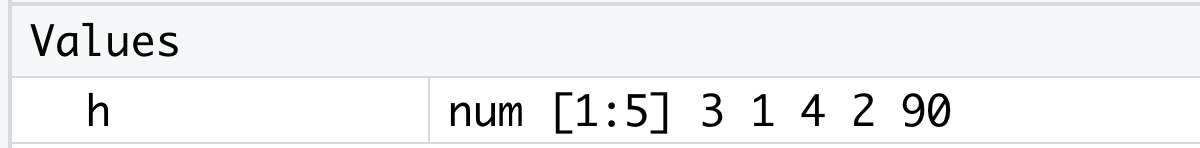
\includegraphics[width=0.7\linewidth]{pics/2h1} 

}

\caption{Values of h (1)}\label{fig:h1}
\end{figure}

Now we all know that \texttt{h} is a numeric vector with 5 values. Then let's try to do an object assignment again, this time you can assign different values to \texttt{h} and see what will happen to \texttt{h}.

\begin{Shaded}
\begin{Highlighting}[]
\NormalTok{h }\OtherTok{\textless{}{-}} \FunctionTok{c}\NormalTok{(}\DecValTok{1}\NormalTok{,}\DecValTok{2}\NormalTok{,}\DecValTok{3}\NormalTok{,}\DecValTok{4}\NormalTok{,}\DecValTok{5}\NormalTok{)}
\NormalTok{h}
\CommentTok{\#\textgreater{} [1] 1 2 3 4 5}
\end{Highlighting}
\end{Shaded}

Then you can see that the values of \texttt{h} have been changed to the new ones! Another easier way to verify values of \texttt{h} is from the environment, so it is a good habit to monitor the environment from time to time to make sure everything look fine.

\begin{figure}

{\centering 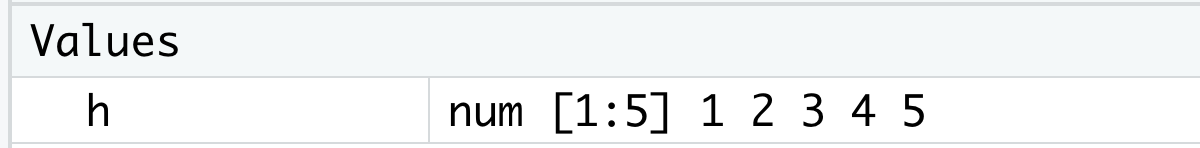
\includegraphics[width=0.7\linewidth]{pics/2h2} 

}

\caption{Values of h (2)}\label{fig:h2}
\end{figure}

You can assign any values to \texttt{h} as you want, then \texttt{h} may change the vector type or even the object type according to the values assigned. By running the following code, \texttt{h} will be a character vector with three strings.

\begin{Shaded}
\begin{Highlighting}[]
\NormalTok{h }\OtherTok{\textless{}{-}} \FunctionTok{c}\NormalTok{(}\StringTok{"pig"}\NormalTok{, }\StringTok{"monkey"}\NormalTok{, }\StringTok{"panda"}\NormalTok{)}
\end{Highlighting}
\end{Shaded}

\begin{figure}

{\centering 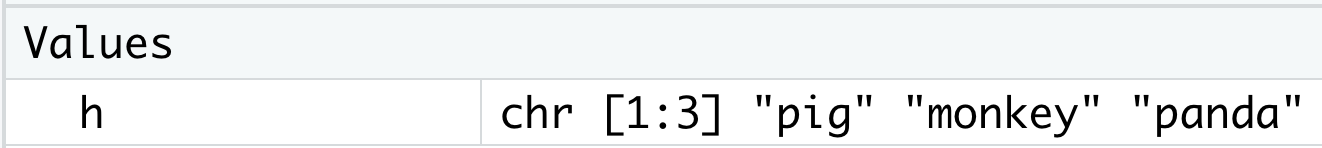
\includegraphics[width=0.7\linewidth]{pics/2h3} 

}

\caption{Values of h (3)}\label{fig:h3}
\end{figure}

\begin{infobox}{caution}

If you assign values of a subvector to a name, you will create a new named vector. Now \texttt{hs} is not the subset of \texttt{h}, it is a vector with the same value as the subset. If you assign different value(s) to \texttt{hs}, there will be no change on \texttt{h}.

\begin{Shaded}
\begin{Highlighting}[]
\NormalTok{h }\OtherTok{\textless{}{-}} \FunctionTok{c}\NormalTok{(}\DecValTok{3}\NormalTok{,}\DecValTok{1}\NormalTok{,}\DecValTok{4}\NormalTok{,}\DecValTok{2}\NormalTok{,}\DecValTok{90}\NormalTok{)}
\NormalTok{hs }\OtherTok{\textless{}{-}}\NormalTok{ h[}\FunctionTok{c}\NormalTok{(}\DecValTok{2}\NormalTok{,}\DecValTok{4}\NormalTok{)]}
\NormalTok{hs }\OtherTok{\textless{}{-}} \DecValTok{10}
\NormalTok{h}
\end{Highlighting}
\end{Shaded}

\end{infobox}

\hypertarget{exercises-8}{%
\subsection{Exercises}\label{exercises-8}}

Consider the vector \texttt{v1\ \textless{}-\ c(7,\ 2,\ 4,\ 9,\ 7)}, \texttt{v2\ \textless{}-\ c(6,\ 2,\ 8,\ 7,\ 9)}, and \texttt{v3\ \textless{}-\ 1:50}.

\begin{enumerate}
\def\labelenumi{\arabic{enumi}.}
\item
  Find the indices in \texttt{v1} where the corresponding value is smaller than \texttt{v2}.
\item
  Find the subvector of \texttt{v2} such that the corresponding location in \texttt{v1} is larger than 5.
\item
  Find the subvector of \texttt{v3} such that it is divisible by 7. (Hint: the result of \texttt{7\%\%7} is equal to 0 since 7 is divisible by 7)
\item
  For all elements of \texttt{v3} that is divisible by 8, replace it by 100.
\end{enumerate}

\hypertarget{logical-operators}{%
\section{Logical Operators}\label{logical-operators}}

In last section, you learned how to do vector subsetting, which yields a subvector of the original vector. Let's take a numeric vector \texttt{x\ \textless{}-\ 1:5} for example. In order to get a subvector of \texttt{x} with values bigger than 3, you can first create a \textbf{logical vector} \texttt{xb3\ \textless{}-\ \ x\ \textgreater{}\ 3}, then use the \texttt{xb3} as the index to do vector subsetting.

\begin{Shaded}
\begin{Highlighting}[]
\NormalTok{x }\OtherTok{\textless{}{-}} \DecValTok{1}\SpecialCharTok{:}\DecValTok{5}
\NormalTok{xb3 }\OtherTok{\textless{}{-}}\NormalTok{ x }\SpecialCharTok{\textgreater{}} \DecValTok{3}
\NormalTok{set1 }\OtherTok{\textless{}{-}}\NormalTok{ x[xb3]}
\NormalTok{set1}
\CommentTok{\#\textgreater{} [1] 4 5}
\end{Highlighting}
\end{Shaded}

Here, the numeric vector \texttt{set1} has values \texttt{4\ 5}. You can get another subvector of \texttt{x} by running the following codes.

\begin{Shaded}
\begin{Highlighting}[]
\NormalTok{xs4 }\OtherTok{\textless{}{-}}\NormalTok{ x }\SpecialCharTok{\textless{}=} \DecValTok{4}
\NormalTok{set2 }\OtherTok{\textless{}{-}}\NormalTok{ x[xs4]}
\end{Highlighting}
\end{Shaded}

Sometimes, you may want to get a subvector with more than one conditions. For example, how can we find the subvector of \texttt{x} with values larger than 3 and less than or equal to 4? In this section, we will introduce several \textbf{logical operators} and use them to get subvectors. Here, we only introduce how to apply these operators on logical vectors.

Before we get started, let's create another numeric vector \texttt{y} and compare it to \texttt{8} and \texttt{9} separately, then you will get two logical vectors with same values as \texttt{xb3} and \texttt{xs4}.

\begin{Shaded}
\begin{Highlighting}[]
\NormalTok{y }\OtherTok{\textless{}{-}} \DecValTok{6}\SpecialCharTok{:}\DecValTok{10}
\NormalTok{yb8 }\OtherTok{\textless{}{-}}\NormalTok{ y }\SpecialCharTok{\textgreater{}} \DecValTok{8}           \CommentTok{\#xb3 is the same as yb8}
\NormalTok{ys9 }\OtherTok{\textless{}{-}}\NormalTok{ y }\SpecialCharTok{\textless{}=} \DecValTok{9}          \CommentTok{\#xs4 is the same as ys9}
\end{Highlighting}
\end{Shaded}

\hypertarget{not-operator-by}{%
\subsection{\texorpdfstring{NOT operator by \texttt{!}}{NOT operator by !}}\label{not-operator-by}}

The first operator we want to introduce is \texttt{!}, often called the \textbf{NOT operator}. Let's see what happens if you apply the NOT operator on a logical vector,

\begin{Shaded}
\begin{Highlighting}[]
\SpecialCharTok{!}\FunctionTok{c}\NormalTok{(}\ConstantTok{FALSE}\NormalTok{, }\ConstantTok{FALSE}\NormalTok{, }\ConstantTok{FALSE}\NormalTok{, }\ConstantTok{TRUE}\NormalTok{, }\ConstantTok{TRUE}\NormalTok{)  }\CommentTok{\#the opposite of a logical vector}
\CommentTok{\#\textgreater{} [1]  TRUE  TRUE  TRUE FALSE FALSE}
\end{Highlighting}
\end{Shaded}

From the result, you get another logical vector with the same length as the original one. The value of each element in the new vector is the \textbf{opposite} of the corresponding value in the original vector. It is intuitive to understand since if something is NOT FALSE, then it is TRUE; and if it is NOT TRUE, then it has to be FALSE.

Since \texttt{xb3} is also a logical vector, you can try to apply \texttt{!} on \texttt{xb3}, and use \texttt{!xb3} (which is also a logical vector) to do vector subsetting. Guess what will you get?

\begin{Shaded}
\begin{Highlighting}[]
\SpecialCharTok{!}\NormalTok{xb3}
\CommentTok{\#\textgreater{} [1]  TRUE  TRUE  TRUE FALSE FALSE}
\NormalTok{set3 }\OtherTok{\textless{}{-}}\NormalTok{ x[}\SpecialCharTok{!}\NormalTok{xb3]}
\NormalTok{set3}
\CommentTok{\#\textgreater{} [1] 1 2 3}
\end{Highlighting}
\end{Shaded}

Of course the resulting numeric vector \texttt{set3} will have \texttt{1\ 2\ 3} as values! As a result, \texttt{set1} and \texttt{set3} are complement of each other from the whole vector \texttt{x}.

From Section \ref{comparison-vector-subsetting}, you have learned that if the logical vectors you use are identical, you will get the same result after doing vector subsetting. So if you use \texttt{!yb8} to do vector subsetting, you will get a vector with the same result as that when you use \texttt{set3}.

\begin{Shaded}
\begin{Highlighting}[]
\NormalTok{x[}\SpecialCharTok{!}\NormalTok{yb8]}
\CommentTok{\#\textgreater{} [1] 1 2 3}
\end{Highlighting}
\end{Shaded}

\hypertarget{and-operator-by}{%
\subsection{\texorpdfstring{AND operator by \texttt{\&}}{AND operator by \&}}\label{and-operator-by}}

Secondly, we will introduce the AND operator \texttt{\&}. Similar to making comparisons between two logical vectors, \texttt{\&} performs comparisons elementwisely, which generates a vector with the same length if the input logical vectors are of the same length or with the same length as that of the longer vector. For each location of the resulting vector, the value will be \texttt{TRUE} if both values in the same location of the input two vectors are \textbf{both \texttt{TRUE}}, and will be \texttt{FALSE} otherwise. In particular, for each element, we have the following summary.

\begin{tabular}{l|l}
\hline
Operation & Result\\
\hline
TRUE \& TRUE & TRUE\\
\hline
TRUE \& FALSE & FALSE\\
\hline
FALSE \& TRUE & FALSE\\
\hline
FALSE \& FALSE & FALSE\\
\hline
\end{tabular}

Let's see an example of the AND operation between two logical vectors of the same length.

\begin{Shaded}
\begin{Highlighting}[]
\FunctionTok{c}\NormalTok{(}\ConstantTok{FALSE}\NormalTok{, }\ConstantTok{FALSE}\NormalTok{, }\ConstantTok{FALSE}\NormalTok{, }\ConstantTok{TRUE}\NormalTok{, }\ConstantTok{TRUE}\NormalTok{) }\SpecialCharTok{\&} \FunctionTok{c}\NormalTok{(}\ConstantTok{TRUE}\NormalTok{, }\ConstantTok{TRUE}\NormalTok{, }\ConstantTok{FALSE}\NormalTok{, }\ConstantTok{TRUE}\NormalTok{, }\ConstantTok{FALSE}\NormalTok{)}
\CommentTok{\#\textgreater{} [1] FALSE FALSE FALSE  TRUE FALSE}
\end{Highlighting}
\end{Shaded}

As explained before, the AND operator works elementwisely and the intermediate step is as below.

\begin{Shaded}
\begin{Highlighting}[]
\FunctionTok{c}\NormalTok{(}\ConstantTok{FALSE} \SpecialCharTok{\&} \ConstantTok{TRUE}\NormalTok{, }\ConstantTok{FALSE} \SpecialCharTok{\&} \ConstantTok{TRUE}\NormalTok{, }\ConstantTok{FALSE} \SpecialCharTok{\&} \ConstantTok{FALSE}\NormalTok{, }\ConstantTok{TRUE} \SpecialCharTok{\&} \ConstantTok{TRUE}\NormalTok{, }\ConstantTok{TRUE} \SpecialCharTok{\&} \ConstantTok{FALSE}\NormalTok{)}
\CommentTok{\#\textgreater{} [1] FALSE FALSE FALSE  TRUE FALSE}
\end{Highlighting}
\end{Shaded}

As you can see from the result, only the fourth element is \texttt{TRUE} since the fourth element of both input logical vectors is \texttt{TRUE}.

Since the AND operator makes comparisons elementwisely, the \emph{recycling rule} also works here. But normally we want one vector with length \textgreater{} 1 and another one with length 1.

\begin{Shaded}
\begin{Highlighting}[]
\FunctionTok{c}\NormalTok{(}\ConstantTok{FALSE}\NormalTok{, }\ConstantTok{FALSE}\NormalTok{, }\ConstantTok{FALSE}\NormalTok{, }\ConstantTok{TRUE}\NormalTok{, }\ConstantTok{TRUE}\NormalTok{) }\SpecialCharTok{\&} \ConstantTok{FALSE}
\CommentTok{\#\textgreater{} [1] FALSE FALSE FALSE FALSE FALSE}
\end{Highlighting}
\end{Shaded}

After learning about the AND operator, you can now get a subvector of \texttt{x} with value(s) \textgreater{} 3 and \textless= 4 easily. At the beginning of this section, you have created two logical vectors \texttt{xb3} and \texttt{xs4} by making comparisons, then let's apply \texttt{\&} on these vectors,

\begin{Shaded}
\begin{Highlighting}[]
\NormalTok{xb3 }\SpecialCharTok{\&}\NormalTok{ xs4  }
\CommentTok{\#\textgreater{} [1] FALSE FALSE FALSE  TRUE FALSE}
\end{Highlighting}
\end{Shaded}

From the result, you know that both \texttt{xb3} and \texttt{xs4} have value \texttt{TRUE} for the fourth element, which means the statement that \emph{the value is \textgreater{} 3 and \textless= 4} is TRUE for the fourth element in \texttt{x}. Then you can use \texttt{xb3\ \&\ xs4} (a logical vector) to do vector subsetting.

\begin{Shaded}
\begin{Highlighting}[]
\NormalTok{x[xb3 }\SpecialCharTok{\&}\NormalTok{ xs4]                                      }
\CommentTok{\#\textgreater{} [1] 4}
\end{Highlighting}
\end{Shaded}

Here, you get a subvector of \texttt{x} with value \texttt{4}.

Since \texttt{xs4} and \texttt{ys9} have same values, you will get the same result if you include \texttt{ys9} to get a subvector. You can try the following codes by yourself.

\begin{Shaded}
\begin{Highlighting}[]
\NormalTok{x[xb3 }\SpecialCharTok{\&}\NormalTok{ ys9]}
\NormalTok{x[yb8 }\SpecialCharTok{\&}\NormalTok{ ys9]}
\end{Highlighting}
\end{Shaded}

Note that the logical vector used to do vector subsetting needs to be of the \textbf{same length} as the original vector. Since \texttt{x} and \texttt{y} have the same length, the logical vectors from above can be used to get subvectors of \texttt{y} as well. You will get the same result from the following four codes.

\begin{Shaded}
\begin{Highlighting}[]
\NormalTok{y[xb3 }\SpecialCharTok{\&}\NormalTok{ xs4]}
\NormalTok{y[yb8 }\SpecialCharTok{\&}\NormalTok{ ys9]}
\NormalTok{y[xb3 }\SpecialCharTok{\&}\NormalTok{ ys9]}
\NormalTok{y[yb8 }\SpecialCharTok{\&}\NormalTok{ xs4]}
\end{Highlighting}
\end{Shaded}

\hypertarget{or-operator-by}{%
\subsection{\texorpdfstring{OR operator by \texttt{\textbar{}}}{OR operator by \textbar{}}}\label{or-operator-by}}

The OR operator \texttt{\textbar{}} works similarly to the AND operator \texttt{\&}, but the difference is that \texttt{\textbar{}} returns \texttt{TRUE} if there is \textbf{at least one} \texttt{TRUE} among the two elements at the same location in two vectors. Let's go through some examples together.

\begin{tabular}{l|l}
\hline
Operation & Result\\
\hline
TRUE | TRUE & TRUE\\
\hline
TRUE | FALSE & TRUE\\
\hline
FALSE | TRUE & TRUE\\
\hline
FALSE | FALSE & FALSE\\
\hline
\end{tabular}

Let's try another example on length \textgreater{} 1 vectors and compare the result with that when we use the AND operator \texttt{\&}.

\begin{Shaded}
\begin{Highlighting}[]
\FunctionTok{c}\NormalTok{(}\ConstantTok{FALSE}\NormalTok{, }\ConstantTok{FALSE}\NormalTok{, }\ConstantTok{FALSE}\NormalTok{, }\ConstantTok{TRUE}\NormalTok{, }\ConstantTok{TRUE}\NormalTok{) }\SpecialCharTok{|} \FunctionTok{c}\NormalTok{(}\ConstantTok{TRUE}\NormalTok{, }\ConstantTok{TRUE}\NormalTok{, }\ConstantTok{FALSE}\NormalTok{, }\ConstantTok{TRUE}\NormalTok{, }\ConstantTok{FALSE}\NormalTok{)}
\CommentTok{\#\textgreater{} [1]  TRUE  TRUE FALSE  TRUE  TRUE}
\FunctionTok{c}\NormalTok{(}\ConstantTok{FALSE}\NormalTok{, }\ConstantTok{FALSE}\NormalTok{, }\ConstantTok{FALSE}\NormalTok{, }\ConstantTok{TRUE}\NormalTok{, }\ConstantTok{TRUE}\NormalTok{) }\SpecialCharTok{\&} \FunctionTok{c}\NormalTok{(}\ConstantTok{TRUE}\NormalTok{, }\ConstantTok{TRUE}\NormalTok{, }\ConstantTok{FALSE}\NormalTok{, }\ConstantTok{TRUE}\NormalTok{, }\ConstantTok{FALSE}\NormalTok{)}
\CommentTok{\#\textgreater{} [1] FALSE FALSE FALSE  TRUE FALSE}
\end{Highlighting}
\end{Shaded}

You also get a length-5 logical vector with an elementwise OR operation \texttt{\textbar{}}, which is very different from the result with AND operation \texttt{\&}.

Of course you can also use \texttt{xb3\ \textbar{}\ xs4} to do vector subsetting, with it being another length-5 logical vector.

\begin{Shaded}
\begin{Highlighting}[]
\NormalTok{x[xb3 }\SpecialCharTok{|}\NormalTok{ xs4]}
\CommentTok{\#\textgreater{} [1] 1 2 3 4 5}
\end{Highlighting}
\end{Shaded}

Wow! You get all five elements of \texttt{x}! That's because the statement ``the value is either \textgreater{} 3 or \textless= 4'' is TRUE for all elements in \texttt{x}.

\hypertarget{exclusive-or-by-xor}{%
\subsection{\texorpdfstring{Exclusive OR by \texttt{xor}}{Exclusive OR by xor}}\label{exclusive-or-by-xor}}

Last but not least, we introduce the \textbf{exclusive OR} operator \texttt{xor}. From the name, it's easy to know that \texttt{xor} is an extended form of \texttt{\textbar{}}. Here are some examples,

\begin{tabular}{l|l}
\hline
Operation & Result\\
\hline
xor(TRUE, TRUE) & FALSE\\
\hline
xor(TRUE, FALSE) & TRUE\\
\hline
xor(FALSE, TRUE) & TRUE\\
\hline
xor(FALSE, FALSE) & FALSE\\
\hline
\end{tabular}

Different from the OR operator, \texttt{xor()} returns \texttt{TRUE} when there is \textbf{one and only one} \texttt{TRUE} among values of these two logical vectors. If these two vectors have the same value, both \texttt{TRUE} or both \texttt{FALSE}, you will get the value \texttt{FALSE}.

For two length \textgreater{} 1 vectors, \texttt{xor()} again performs comparisons elementwisely. You can check the result by yourself!

\begin{Shaded}
\begin{Highlighting}[]
\FunctionTok{xor}\NormalTok{(}\FunctionTok{c}\NormalTok{(}\ConstantTok{FALSE}\NormalTok{, }\ConstantTok{FALSE}\NormalTok{, }\ConstantTok{FALSE}\NormalTok{, }\ConstantTok{TRUE}\NormalTok{, }\ConstantTok{TRUE}\NormalTok{), }\FunctionTok{c}\NormalTok{(}\ConstantTok{TRUE}\NormalTok{, }\ConstantTok{TRUE}\NormalTok{, }\ConstantTok{TRUE}\NormalTok{, }\ConstantTok{TRUE}\NormalTok{, }\ConstantTok{FALSE}\NormalTok{))}
\CommentTok{\#\textgreater{} [1]  TRUE  TRUE  TRUE FALSE  TRUE}
\end{Highlighting}
\end{Shaded}

Since you also get a logical vector after applying \texttt{xor()}, you can use it to do vector subsetting. Using different combinations to do vector subsetting is interesting. Try them!

\begin{Shaded}
\begin{Highlighting}[]
\NormalTok{x[}\FunctionTok{xor}\NormalTok{(xb3, xs4)]}
\NormalTok{y[}\FunctionTok{xor}\NormalTok{(}\SpecialCharTok{!}\NormalTok{xb3, ys9)]}
\NormalTok{y[}\FunctionTok{xor}\NormalTok{(yb8, }\SpecialCharTok{!}\NormalTok{ys9)]}
\end{Highlighting}
\end{Shaded}

\hypertarget{summary-of-logical-operators}{%
\subsection{Summary of Logical Operators}\label{summary-of-logical-operators}}

Let's summarize the logical operators between two vectors.

\begin{itemize}
\tightlist
\item
  The NOT operator \texttt{!} gives the opposite of each value.
\item
  The AND operator \texttt{\&} returns \texttt{TRUE} if both are \texttt{TRUE}.
\item
  The OR operator \texttt{\textbar{}} returns \texttt{TRUE} if at least one is \texttt{TRUE}.
\item
  The exclusive OR operator \texttt{xor()} returns \texttt{TRUE} if one and only one is \texttt{TRUE}.
\end{itemize}

\hypertarget{exercises-9}{%
\subsection{Exercises}\label{exercises-9}}

Consider the vector \texttt{v1\ \textless{}-\ seq(from\ =\ 1,\ to\ =\ 100,\ by\ =\ 3)}, and \texttt{v2\ \textless{}-\ \ sqrt(v1)}.

\begin{enumerate}
\def\labelenumi{\arabic{enumi}.}
\item
  Find the subvector of \texttt{v1} with values bigger or equal to 30 and less than 60. And assign the subvector to name v1s.
\item
  Find the subvector of \texttt{v2} such that the corresponding value of \texttt{v1} is less than 20 or larger than 50.
\item
  Use an example to verify \(xor(a, b) = (!a & b) | (a & !b)\)
\end{enumerate}

\hypertarget{set-operations-between-two-vectors}{%
\section{Set Operations between two vectors}\label{set-operations-between-two-vectors}}

In Section \ref{logical-operators}, we introduced logical operators which are operators between two logical vectors. In this section, we will discuss set operations between two vectors of the \textbf{same type}. Note that while the logical operators only make sense for logical vectors, the operations we will introduce work for all three kinds of vectors. In the rest of this section, we will introduce several operations one by one.

\hypertarget{operations}{%
\subsection{Numeric vectors}\label{operations}}

Let's start with numeric vectors. Firstly, let's create two numeric vectors \texttt{x} and \texttt{y}.

\begin{Shaded}
\begin{Highlighting}[]
\NormalTok{x }\OtherTok{\textless{}{-}} \FunctionTok{c}\NormalTok{(}\DecValTok{1}\NormalTok{, }\DecValTok{2}\NormalTok{, }\DecValTok{1}\NormalTok{, }\DecValTok{3}\NormalTok{, }\DecValTok{1}\NormalTok{)}
\NormalTok{y }\OtherTok{\textless{}{-}} \FunctionTok{c}\NormalTok{(}\DecValTok{1}\NormalTok{, }\DecValTok{1}\NormalTok{, }\DecValTok{3}\NormalTok{, }\DecValTok{4}\NormalTok{, }\DecValTok{4}\NormalTok{, }\DecValTok{5}\NormalTok{)}
\end{Highlighting}
\end{Shaded}

\textbf{\emph{a. Intersection}}\\
To get values in both \texttt{x} and \texttt{y}, you can use the \texttt{intersect()} function.

\begin{Shaded}
\begin{Highlighting}[]
\FunctionTok{intersect}\NormalTok{(x, y)}
\CommentTok{\#\textgreater{} [1] 1 3}
\end{Highlighting}
\end{Shaded}

Note that although \texttt{x} has three elements of \texttt{1} and \texttt{y} has two, the result of their intersection only has one \texttt{1}, showing that only the \textbf{unique elements} are retained in the output.

\textbf{\emph{b. Union}}\\
To get values in either \texttt{x} or \texttt{y}, you can use the \texttt{union()} function.

\begin{Shaded}
\begin{Highlighting}[]
\FunctionTok{union}\NormalTok{(x, y)}
\CommentTok{\#\textgreater{} [1] 1 2 3 4 5}
\end{Highlighting}
\end{Shaded}

Again, only one copy of each value is retained in the output.

\textbf{\emph{c.~Set difference}}\\
To get values in \texttt{x} but not in \texttt{y}, you can use the \texttt{setdiff()} function. Notice that \texttt{x} is in the first argument and \texttt{y} is in the second in this situation.

\begin{Shaded}
\begin{Highlighting}[]
\FunctionTok{setdiff}\NormalTok{(x, y)}
\CommentTok{\#\textgreater{} [1] 2}
\end{Highlighting}
\end{Shaded}

Then you will get the result of \texttt{2}! But you may be wondering why you don't get \texttt{1\ 2} as the result since there is one more \texttt{1} in \texttt{x} than in \texttt{y}? That's because for this operation, you will get unique elements of \texttt{x} and \texttt{y} firstly, then find the set difference between them.

Similarly, if you want to get values in \texttt{y} but not in \texttt{x}, \texttt{y} should be in the first argument and \texttt{x} is in the second.

\begin{Shaded}
\begin{Highlighting}[]
\FunctionTok{setdiff}\NormalTok{(y, x)}
\CommentTok{\#\textgreater{} [1] 4 5}
\end{Highlighting}
\end{Shaded}

\textbf{\emph{d.~Set equality}}\\
To check whether the two vectors \texttt{x} and \texttt{y} are the same, you can use the \texttt{setequal()} function.

\begin{Shaded}
\begin{Highlighting}[]
\FunctionTok{setequal}\NormalTok{(x, y)}
\CommentTok{\#\textgreater{} [1] FALSE}
\end{Highlighting}
\end{Shaded}

Of course you will get \texttt{FALSE} since \texttt{x} has value \texttt{2} which \texttt{y} doesn't have.

Similar to the \texttt{setdiff()} function, the \texttt{setequal()} function works by looking at whether the two vectors have same set of unique values. For example, you will get \texttt{TRUE} in the following example,

\begin{Shaded}
\begin{Highlighting}[]
\FunctionTok{setequal}\NormalTok{(}\FunctionTok{c}\NormalTok{(}\DecValTok{1}\NormalTok{, }\DecValTok{1}\NormalTok{, }\DecValTok{2}\NormalTok{), }\FunctionTok{c}\NormalTok{(}\DecValTok{1}\NormalTok{, }\DecValTok{2}\NormalTok{))}
\CommentTok{\#\textgreater{} [1] TRUE}
\end{Highlighting}
\end{Shaded}

\textbf{\emph{e. Membership determination}}\\
To check whether each element of \texttt{x} is inside \texttt{y}, you can use the \texttt{is.element()} function or the \texttt{\%in\%} operator.

\begin{Shaded}
\begin{Highlighting}[]
\FunctionTok{is.element}\NormalTok{(x, y)}
\CommentTok{\#\textgreater{} [1]  TRUE FALSE  TRUE  TRUE  TRUE}
\NormalTok{x }\SpecialCharTok{\%in\%}\NormalTok{ y}
\CommentTok{\#\textgreater{} [1]  TRUE FALSE  TRUE  TRUE  TRUE}
\end{Highlighting}
\end{Shaded}

In this example, it returns a logical vector of length-5, the same length as \texttt{x}. The first element of \texttt{x} is \texttt{1}, and \texttt{y} also has elements with value 1, so the first element of the logical vector is \texttt{TRUE}. The second element of \texttt{x} is \texttt{2}, but \texttt{y} doesn't have any elements with value 2, hence the result is \texttt{FALSE}. You can verify the other elements by yourself.

The order of vectors is important for membership determination since if you put \texttt{y} before \texttt{x}, you will check whether each element of \texttt{y} is inside \texttt{x}.

\begin{Shaded}
\begin{Highlighting}[]
\FunctionTok{is.element}\NormalTok{(y, x)}
\CommentTok{\#\textgreater{} [1]  TRUE  TRUE  TRUE FALSE FALSE FALSE}
\NormalTok{y }\SpecialCharTok{\%in\%}\NormalTok{ x}
\CommentTok{\#\textgreater{} [1]  TRUE  TRUE  TRUE FALSE FALSE FALSE}
\end{Highlighting}
\end{Shaded}

Please find a summary of the set operations between \texttt{x} and \texttt{y} in the following table.

\begin{tabular}{l|l}
\hline
Operation & Code\\
\hline
Intersection & `intersect(x, y)`\\
\hline
Union & `union(x, y)`\\
\hline
Set Difference & `setdiff(x, y)`\\
\hline
Set Equality & `setequal(x, y)`\\
\hline
Membership Determination & `is.element(x, y)`\\
\hline
\end{tabular}

\hypertarget{character-vectors-1}{%
\subsection{Character vectors}\label{character-vectors-1}}

Now you must have been familiar with all the five operations! Similar to numeric vectors, you can also apply operations on character vectors. Here are some codes which you can run by yourself.

\begin{Shaded}
\begin{Highlighting}[]
\NormalTok{a }\OtherTok{\textless{}{-}} \FunctionTok{c}\NormalTok{(}\StringTok{"sheep"}\NormalTok{, }\StringTok{"monkey"}\NormalTok{, }\StringTok{"sheep"}\NormalTok{, }\StringTok{"chicken"}\NormalTok{, }\StringTok{"dragon"}\NormalTok{)}
\NormalTok{b }\OtherTok{\textless{}{-}} \FunctionTok{c}\NormalTok{(}\StringTok{"sheep"}\NormalTok{, }\StringTok{"pig"}\NormalTok{, }\StringTok{"pig"}\NormalTok{)}
\FunctionTok{intersect}\NormalTok{(a, b)}
\FunctionTok{union}\NormalTok{(a, b)}
\FunctionTok{setdiff}\NormalTok{(a, b)}
\FunctionTok{setequal}\NormalTok{(a, b)}
\NormalTok{a }\SpecialCharTok{\%in\%}\NormalTok{ b}
\end{Highlighting}
\end{Shaded}

\hypertarget{logical-vectors-1}{%
\subsection{Logical vectors}\label{logical-vectors-1}}

Of course you can also apply set operations on logical vectors.

\begin{Shaded}
\begin{Highlighting}[]
\NormalTok{c }\OtherTok{\textless{}{-}} \FunctionTok{c}\NormalTok{(}\StringTok{"T"}\NormalTok{, }\StringTok{"F"}\NormalTok{, }\StringTok{"F"}\NormalTok{, }\StringTok{"T"}\NormalTok{)}
\NormalTok{d }\OtherTok{\textless{}{-}} \FunctionTok{c}\NormalTok{(}\StringTok{"T"}\NormalTok{, }\StringTok{"T"}\NormalTok{, }\StringTok{"T"}\NormalTok{)}
\FunctionTok{intersect}\NormalTok{(c, d)}
\FunctionTok{union}\NormalTok{(c, d)}
\FunctionTok{setdiff}\NormalTok{(c, d)}
\FunctionTok{setequal}\NormalTok{(c, d)}
\NormalTok{c }\SpecialCharTok{\%in\%}\NormalTok{ d}
\end{Highlighting}
\end{Shaded}

\hypertarget{exercises-10}{%
\subsection{Exercises}\label{exercises-10}}

Consider the vector \texttt{s1\ \textless{}-\ seq(from\ =\ 1,\ to\ =\ 100,\ length.out\ =\ 7)}.

\begin{enumerate}
\def\labelenumi{\arabic{enumi}.}
\item
  Compare \texttt{s1} to 50 to see whether the values of \texttt{s1} are bigger than 50, then assign the result to name s2. Compare \texttt{s1} to 80 to see whether the values of \texttt{s1} are less or equal to 80, then assign the result to name s3.
\item
  Use two methods (logical operators and set operations) to find the subvector of \texttt{s1} with values bigger than 50 and less or equal to 80.
\item
  For \texttt{x\ \textless{}-\ 1:200}, use two methods (logical operators and set operations) to find the subvector of \texttt{x} that is divisible by 7, but not divisible by 2.
\end{enumerate}

\hypertarget{summary-of-operators}{%
\section{Summary of Operators}\label{summary-of-operators}}

Now we have fully introduced the first object----\textbf{vectors}. You have learned how to create vectors and apply various operations on them. There are several different types of \textbf{operators} to conduct different \textbf{operations} in R. In this section, we want to give you a brief review of some operators and operations according to their types.

Let's summarize the four types of operators we have learned. In the following parts, we will review each type one by one.

\begin{tabular}{l|l}
\hline
Operator & Section\\
\hline
arithmetic operator & \textbackslash{}@ref(Calculator)\\
\hline
assignment operator & \textbackslash{}@ref(Object-Assignment)\\
\hline
relational operator & \textbackslash{}@ref(comparison-vector-subsetting)\\
\hline
logical operator & \textbackslash{}@ref(logical-operators)\\
\hline
\end{tabular}

\hypertarget{arithmetic-operator}{%
\subsection{Arithmetic operator}\label{arithmetic-operator}}

\textbf{Arithmetic operators} (Section \ref{Calculator}) are operators that often used to some basic calculations. The following is a list of operators available in R.

\begin{tabular}{l|l}
\hline
Operator & Explanation\\
\hline
+ & addition\\
\hline
- & subtraction\\
\hline
* & multiplication\\
\hline
/ & division\\
\hline
\%/\% & integer division\\
\hline
\%\% & modulus\\
\hline
\textasciicircum{} & exponentiation\\
\hline
\end{tabular}

\hypertarget{assignment-operator}{%
\subsection{Assignment operator}\label{assignment-operator}}

The \textbf{assignment operator} (Section \ref{Object-Assignment}) is the perhaps the most fundamental operator. It can help you to create objects with names.

\begin{tabular}{l|l}
\hline
Operator & Explanation\\
\hline
<- & do object assignment\\
\hline
\end{tabular}

\hypertarget{relational-operator}{%
\subsection{Relational operator}\label{relational-operator}}

\textbf{Relational operators} are operators that are often used to do comparisons. The following is a list of operators available in R.

\begin{tabular}{l|l}
\hline
Operator & Explanation\\
\hline
< & less\\
\hline
<= & less than or equal to\\
\hline
> & bigger\\
\hline
>= & bigger than or equal to\\
\hline
== & equal to\\
\hline
!= & not equal to\\
\hline
\end{tabular}

\hypertarget{logical-operator}{%
\subsection{Logical operator}\label{logical-operator}}

\textbf{Logical operators} are often used between two logical vectors when we want to do a particular vector subsetting. The following is a list of logical operators available in R.

\begin{tabular}{l|l}
\hline
Operator & Explanation\\
\hline
! & NOT\\
\hline
\& & AND\\
\hline
| & OR\\
\hline
xor() & Exculsive OR\\
\hline
\end{tabular}

In addition to using various operators to conduct operations, we can do much more using various functions in R.

\hypertarget{na}{%
\section{Missing Values (NA)}\label{na}}

In applications, you may encounter the situation where some values are missing in the data set. In this scenario, R uses \texttt{NA} to represent those values, indicating they are \textbf{not available}. Let's see the following example.

\begin{Shaded}
\begin{Highlighting}[]
\NormalTok{a }\OtherTok{\textless{}{-}} \DecValTok{1}\SpecialCharTok{:}\DecValTok{10}
\NormalTok{a[}\DecValTok{11}\NormalTok{]}
\CommentTok{\#\textgreater{} [1] NA}
\end{Highlighting}
\end{Shaded}

Since you have defined \texttt{a} as a vector of length 10, there are 10 values in \texttt{a}. If you try to access the 11th element of \texttt{a}, it is not available, hence you will see \texttt{NA} as the result.

Sometimes, the values of some elements in a vector are missing, then you can use \texttt{NA} for these elements. Here is an example containing \texttt{NA}s in values. If you want to get values of the 2nd and 4th elements in \texttt{b}, of course you will get \texttt{NA\ NA} as the result.

\begin{Shaded}
\begin{Highlighting}[]
\NormalTok{b }\OtherTok{\textless{}{-}} \FunctionTok{c}\NormalTok{(}\DecValTok{1}\NormalTok{, }\ConstantTok{NA}\NormalTok{, }\DecValTok{2}\NormalTok{, }\ConstantTok{NA}\NormalTok{, }\DecValTok{3}\NormalTok{)}
\NormalTok{b}
\CommentTok{\#\textgreater{} [1]  1 NA  2 NA  3}
\NormalTok{b[}\FunctionTok{c}\NormalTok{(}\DecValTok{2}\NormalTok{,}\DecValTok{4}\NormalTok{)]}
\CommentTok{\#\textgreater{} [1] NA NA}
\end{Highlighting}
\end{Shaded}

Now you have had a basic understanding of \texttt{NA}. In the following parts of this section, we want to introduce several properties of \texttt{NA}. Let's start with \texttt{NA} is contagious.

\hypertarget{na-is-contagious}{%
\subsection{\texorpdfstring{\texttt{NA} is contagious}{NA is contagious}}\label{na-is-contagious}}

\texttt{NA} implies that the underlying value is not available, in other words, there is uncertainty with the value. As a result, for most operations associated with \texttt{NA}, the results will also be \texttt{NA}, showing that \texttt{NA} is \textbf{contagious}.

\begin{Shaded}
\begin{Highlighting}[]
\NormalTok{y }\OtherTok{\textless{}{-}} \ConstantTok{NA}
\NormalTok{y }\SpecialCharTok{+} \DecValTok{3}
\CommentTok{\#\textgreater{} [1] NA}
\NormalTok{y }\SpecialCharTok{==} \DecValTok{3}
\CommentTok{\#\textgreater{} [1] NA}
\end{Highlighting}
\end{Shaded}

As you can see here, \texttt{y} is \texttt{NA}, indicating the value of \texttt{y} is not available. When you try to do operations like \texttt{y\ +\ 3} or \texttt{y\ ==\ 3}, the answers are clearly not available as well, hence both taking the value \texttt{NA}.

How about we create another \texttt{NA} object and compare it with \texttt{y}?

\begin{Shaded}
\begin{Highlighting}[]
\NormalTok{z }\OtherTok{\textless{}{-}} \ConstantTok{NA} 
\NormalTok{y }\SpecialCharTok{==}\NormalTok{ z }
\CommentTok{\#\textgreater{} [1] NA}
\end{Highlighting}
\end{Shaded}

It is again \texttt{NA}, which may be confusing at first. However, keep in mind that since both \texttt{y} and \texttt{z} are not available, there is no way to tell whether they are the same. Hence \texttt{y\ ==\ z} is also \texttt{NA}.

\begin{infobox}{caution}

\begin{enumerate}
\def\labelenumi{\arabic{enumi}.}
\item
  Think about what is the value of 1\textsuperscript{NA} in R. Try to run it in R. Does it agree with your thoughts?
\item
  Think about what is the value of 0\textsuperscript{NA} in R. Try to run it in R. Does it agree with your thoughts?
\end{enumerate}

\begin{itemize}
\tightlist
\item
  Answer 1. For any \(x\), we have \(1^x = \exp(\log (1^x)) = \exp(x \log 1) = \exp(x \cdot 0) = 1\). Since there is no uncertainty regarding the expression, the value of 1\textsuperscript{NA} is 1
\item
  Answer 2. We have \(0^0 = \lim_{x\to 0}x^x =\exp[\lim_{x\to 0} x\log(x)]=\exp[0] = 1\), and \(0^1 = 0\). Since \texttt{NA} represents uncertainty values, it can be 0 or 1 or other numbers. So 0\textsuperscript{NA} is not deterministic because it can take different values according to the exponent. Hence, the value of 0\textsuperscript{NA} is also \texttt{NA}.
\end{itemize}

\end{infobox}

Now, let's talk about what impact the \texttt{NA} values make when we apply statistical functions. Let's create a vector containing \texttt{NA} values, and apply some functions on it.

\begin{Shaded}
\begin{Highlighting}[]
\NormalTok{x }\OtherTok{\textless{}{-}} \FunctionTok{c}\NormalTok{(}\DecValTok{1}\NormalTok{, }\ConstantTok{NA}\NormalTok{, }\DecValTok{3}\NormalTok{, }\DecValTok{4}\NormalTok{, }\ConstantTok{NA}\NormalTok{, }\DecValTok{2}\NormalTok{)}
\NormalTok{x}
\CommentTok{\#\textgreater{} [1]  1 NA  3  4 NA  2}
\FunctionTok{sum}\NormalTok{(x) }
\CommentTok{\#\textgreater{} [1] NA}
\FunctionTok{mean}\NormalTok{(x)}
\CommentTok{\#\textgreater{} [1] NA}
\FunctionTok{sd}\NormalTok{(x)}
\CommentTok{\#\textgreater{} [1] NA}
\end{Highlighting}
\end{Shaded}

As you can see, for many statistical functions on vectors, as long as there exists at least one \texttt{NA} values in vectors, the results are often impossible to determine, hence resulting an \texttt{NA} value as well.

As a result, you may want to ignore the \texttt{NA} values during the function evaluation. Fortunately, most statistical functions on vectors provide an optional argument \texttt{na.rm}, which takes a logical value, indicating whether to remove \texttt{NA} before applying the functions. Let's see the following examples.

\begin{Shaded}
\begin{Highlighting}[]
\FunctionTok{sum}\NormalTok{(x, }\AttributeTok{na.rm =} \ConstantTok{TRUE}\NormalTok{) }
\CommentTok{\#\textgreater{} [1] 10}
\FunctionTok{mean}\NormalTok{(x, }\AttributeTok{na.rm =} \ConstantTok{TRUE}\NormalTok{)}
\CommentTok{\#\textgreater{} [1] 2.5}
\FunctionTok{sd}\NormalTok{(x, }\AttributeTok{na.rm =} \ConstantTok{TRUE}\NormalTok{)}
\CommentTok{\#\textgreater{} [1] 1.290994}
\end{Highlighting}
\end{Shaded}

It is easy to verify that the results are what we expect to get if the \texttt{NA} values are removed. Feel free to try the following codes which apply the same functions on the subvector with the non-missing values.

\begin{Shaded}
\begin{Highlighting}[]
\NormalTok{x\_no\_na }\OtherTok{\textless{}{-}} \FunctionTok{c}\NormalTok{(}\DecValTok{1}\NormalTok{, }\DecValTok{3}\NormalTok{, }\DecValTok{4}\NormalTok{, }\DecValTok{2}\NormalTok{)}
\FunctionTok{sum}\NormalTok{(x\_no\_na) }
\FunctionTok{mean}\NormalTok{(x\_no\_na)}
\FunctionTok{sd}\NormalTok{(x\_no\_na)}
\end{Highlighting}
\end{Shaded}

Interesting, the \texttt{summary()} function will deal with the \texttt{NA} values automatically by removing them before computing the five percentiles and the mean. In addition, the \texttt{summary()} function provides a column which shows the number of \texttt{NA}s in \texttt{x}.

\begin{Shaded}
\begin{Highlighting}[]
\FunctionTok{summary}\NormalTok{(x) }
\CommentTok{\#\textgreater{}    Min. 1st Qu.  Median    Mean 3rd Qu.    Max.    NA\textquotesingle{}s }
\CommentTok{\#\textgreater{}    1.00    1.75    2.50    2.50    3.25    4.00       2}
\end{Highlighting}
\end{Shaded}

\hypertarget{work-with-na-values}{%
\subsection{\texorpdfstring{Work with \texttt{NA} values}{Work with NA values}}\label{work-with-na-values}}

When there are \texttt{NA} values in our vector, there is nothing to be afraid of as there are many useful tools we can use.

Let's use \texttt{x\ \textless{}-\ c(1,\ NA,\ 3,\ 4,\ NA,\ 2)} throughout this part.

\textbf{\emph{a. Find indices with missing values}}

Firstly, we will introduce how to find indices with missing values. To find the indices, you may be tempted to use the comparison operator introduced in Section \ref{comparison-vector-subsetting}. Let's try to compare \texttt{x} with \texttt{NA} as the following code.

\begin{Shaded}
\begin{Highlighting}[]
\NormalTok{x }\SpecialCharTok{==} \ConstantTok{NA}
\end{Highlighting}
\end{Shaded}

You get a vector of all values equaling \texttt{NA}! This is actually not surprising for the following reason. Given that the \texttt{NA} you are comparing can take any unknown value, any comparison with it will result in an \texttt{NA} value due to the lack of information.

Instead of using \texttt{==} for finding missing values, the correct way is to use the \texttt{is.na()} function, which returns a logical vector \texttt{x\_na} representing whether the value of each element is missing or not. Then, you can use the \texttt{which()} function which can return the locations of all \texttt{TRUE} values to find the indices for the \texttt{NA} values. Here, the \texttt{sum()} function on the logical vector \texttt{x\_na} returns the number of \texttt{NA} values in the vector, following the cocercion rule described in Section \ref{func-logical-vector}.

\begin{Shaded}
\begin{Highlighting}[]
\NormalTok{x\_na }\OtherTok{\textless{}{-}} \FunctionTok{is.na}\NormalTok{(x)        }\CommentTok{\#logical vector     }
\NormalTok{x\_na}
\CommentTok{\#\textgreater{} [1] FALSE  TRUE FALSE FALSE  TRUE FALSE}
\FunctionTok{which}\NormalTok{(x\_na)             }\CommentTok{\#numeric vector}
\CommentTok{\#\textgreater{} [1] 2 5}
\FunctionTok{sum}\NormalTok{(x\_na)               }\CommentTok{\#the number of NAs in x }
\CommentTok{\#\textgreater{} [1] 2}
\FunctionTok{sum}\NormalTok{(}\SpecialCharTok{!}\NormalTok{x\_na)              }\CommentTok{\#the number of non{-}NAs in x}
\CommentTok{\#\textgreater{} [1] 4}
\end{Highlighting}
\end{Shaded}

If you only want to detect whether there is any \texttt{NA} values in the vector, you can use the \texttt{anyNA()} function.

\begin{Shaded}
\begin{Highlighting}[]
\FunctionTok{anyNA}\NormalTok{(}\FunctionTok{c}\NormalTok{(}\ConstantTok{NA}\NormalTok{, }\DecValTok{1}\NormalTok{))}
\CommentTok{\#\textgreater{} [1] TRUE}
\FunctionTok{anyNA}\NormalTok{(}\DecValTok{1}\SpecialCharTok{:}\DecValTok{3}\NormalTok{)}
\CommentTok{\#\textgreater{} [1] FALSE}
\end{Highlighting}
\end{Shaded}

\textbf{\emph{b. Remove missing values}}

Sometimes, you may want to simply remove the missing values. To do that, you can use a logical vector to do vector subsetting as introduced in Section \ref{vector-subsetting}. The specific logical vector you want to use is the opposite (\texttt{!}) of the logical vector that represents missing values. Then you will get a subvector of \texttt{x} which keeps all values except \texttt{NA}.

\begin{Shaded}
\begin{Highlighting}[]
\NormalTok{x2 }\OtherTok{\textless{}{-}}\NormalTok{ x[}\SpecialCharTok{!}\NormalTok{x\_na]}
\NormalTok{x2}
\CommentTok{\#\textgreater{} [1] 1 3 4 2}
\end{Highlighting}
\end{Shaded}

\textbf{\emph{c.~Impute missing values}}

In many applications, naively removing the missing values before doing the analysis may lead to incorrect inference. Usually, it is useful to make the data complete by \textbf{imputing} the missing values. For example, you can use mean imputing or median imputing, which replaces the missing values with the mean or median of the non-missing values.

\begin{Shaded}
\begin{Highlighting}[]
\NormalTok{x\_impute }\OtherTok{\textless{}{-}}\NormalTok{ x}
\FunctionTok{mean}\NormalTok{(x, }\AttributeTok{na.rm =} \ConstantTok{TRUE}\NormalTok{)}
\CommentTok{\#\textgreater{} [1] 2.5}
\NormalTok{x\_impute[x\_na] }\OtherTok{\textless{}{-}} \FunctionTok{mean}\NormalTok{(x, }\AttributeTok{na.rm =} \ConstantTok{TRUE}\NormalTok{)}
\NormalTok{x\_impute}
\CommentTok{\#\textgreater{} [1] 1.0 2.5 3.0 4.0 2.5 2.0}
\NormalTok{x}
\CommentTok{\#\textgreater{} [1]  1 NA  3  4 NA  2}
\end{Highlighting}
\end{Shaded}

\begin{infobox}{caution}
If you want to compare the values of an object before and after some operations, you can create a new object with the same value as the original object (here, we create \texttt{x\_impute} which has the same value as \texttt{x}), then make operations on \texttt{x\_impute} without changing the value of \texttt{x}.

\end{infobox}

In \texttt{x\_impute}, values of the 2nd and 5th elements are replaced by 2.5, the average of the non-missing values of \texttt{x}.

\textbf{\emph{d.~Replace non-standard missing values with \texttt{NA} in the vector}}

Sometimes, the data we collected may not use \texttt{NA} to indicate missingness. For example, in the following vector \texttt{x3}, the value \texttt{999} represents the corresponding element is missing.

\begin{Shaded}
\begin{Highlighting}[]
\NormalTok{x3 }\OtherTok{\textless{}{-}} \FunctionTok{c}\NormalTok{(}\DecValTok{4}\NormalTok{, }\DecValTok{999}\NormalTok{, }\DecValTok{1}\NormalTok{, }\DecValTok{999}\NormalTok{, }\DecValTok{3}\NormalTok{, }\DecValTok{999}\NormalTok{, }\DecValTok{999}\NormalTok{)}
\end{Highlighting}
\end{Shaded}

It is highly recommended to convert the values into \texttt{NA} before carrying out any analysis.

\begin{Shaded}
\begin{Highlighting}[]
\NormalTok{x3[x3 }\SpecialCharTok{==} \DecValTok{999}\NormalTok{] }\OtherTok{\textless{}{-}} \ConstantTok{NA}
\NormalTok{x3}
\CommentTok{\#\textgreater{} [1]  4 NA  1 NA  3 NA NA}
\end{Highlighting}
\end{Shaded}

Let's see another example where both \texttt{999} and \texttt{-999} represent the value is missing. You can convert all \texttt{999} and \texttt{-999} into \texttt{NA} by using operations introduced in Section \ref{operations}

\begin{Shaded}
\begin{Highlighting}[]
\NormalTok{x4 }\OtherTok{\textless{}{-}} \FunctionTok{c}\NormalTok{(}\DecValTok{4}\NormalTok{, }\DecValTok{999}\NormalTok{, }\DecValTok{1}\NormalTok{, }\SpecialCharTok{{-}}\DecValTok{999}\NormalTok{, }\DecValTok{3}\NormalTok{, }\SpecialCharTok{{-}}\DecValTok{999}\NormalTok{, }\DecValTok{999}\NormalTok{)}
\DocumentationTok{\#\#999 and {-}999 are the values indicating missingness}
\NormalTok{x4[x4 }\SpecialCharTok{\%in\%} \FunctionTok{c}\NormalTok{(}\DecValTok{999}\NormalTok{, }\SpecialCharTok{{-}}\DecValTok{999}\NormalTok{)] }\OtherTok{\textless{}{-}} \ConstantTok{NA}
\NormalTok{x4}
\CommentTok{\#\textgreater{} [1]  4 NA  1 NA  3 NA NA}
\end{Highlighting}
\end{Shaded}

\hypertarget{exercises-11}{%
\subsection{Exercises}\label{exercises-11}}

\begin{enumerate}
\def\labelenumi{\arabic{enumi}.}
\tightlist
\item
  For the vector \texttt{x\ \textless{}-\ rep(c(1,\ 2,\ NA),\ 3:5)},
\end{enumerate}

\begin{enumerate}
\def\labelenumi{\alph{enumi}.}
\tightlist
\item
  verify each value of \texttt{summary(x)} by using other functions.
\item
  find the indices with missing values;
\item
  create a vector x\_no\_na containing the non-missing values in \texttt{x};
\item
  replace those missing values by the median of the non-missing values in \texttt{x}.
\end{enumerate}

\begin{enumerate}
\def\labelenumi{\arabic{enumi}.}
\setcounter{enumi}{1}
\tightlist
\item
  For the vector \texttt{y\ \textless{}-\ rep(c("N",\ 2,\ "A"),\ 5:3)}, the values of both \texttt{"N"} and \texttt{"A"} indicate missingness. Convert non-standard missing values to \texttt{NA}, then find the indices of \texttt{y} that correspond to missing values.
\end{enumerate}

\hypertarget{dates}{%
\section{Dates and Times}\label{dates}}

Now you have learned numeric vectors, character vectors and logical vectors which are quite intuitive. In this section, we want to introduce two special formats of vectors in R which are \textbf{dates} and \textbf{times}. Dates and times belong to vectors because they only contain values of the same type.

\hypertarget{dates-1}{%
\subsection{Dates}\label{dates-1}}

\textbf{\emph{a. Date class}}

Let's first look at the date format of vector. First, to get today's date, you can use the \texttt{Sys.Date()} function. Similarly, you can verify the vector type by using the \texttt{class()} function.

\begin{Shaded}
\begin{Highlighting}[]
\NormalTok{today }\OtherTok{\textless{}{-}} \FunctionTok{Sys.Date}\NormalTok{()}
\NormalTok{today}
\CommentTok{\#\textgreater{} [1] "2021{-}09{-}29"}
\FunctionTok{class}\NormalTok{(today)}
\CommentTok{\#\textgreater{} [1] "Date"}
\end{Highlighting}
\end{Shaded}

Looking at the output, it appears that \texttt{today} is a vector of \textbf{Date} class, which makes working with dates a piece of cake. For example, you can use \texttt{today\ -\ 1} to get the date of yesterday, and use \texttt{today\ +\ 1} to get the date of tomorrow.

\begin{Shaded}
\begin{Highlighting}[]
\NormalTok{today }\SpecialCharTok{{-}} \DecValTok{1}
\CommentTok{\#\textgreater{} [1] "2021{-}09{-}28"}
\NormalTok{today }\SpecialCharTok{+} \DecValTok{1}
\CommentTok{\#\textgreater{} [1] "2021{-}09{-}30"}
\end{Highlighting}
\end{Shaded}

You can also get the days of week for a date using the \texttt{weekdays()} function.

\begin{Shaded}
\begin{Highlighting}[]
\FunctionTok{weekdays}\NormalTok{(today)}
\end{Highlighting}
\end{Shaded}

\begin{infobox}{caution}

Although the output of \texttt{today} looks similar to a string, you will get a character vector if you assign value(s) like \texttt{"2021-09-09"} to a name, you can verify the vector type by using \texttt{class()}.
Of course an error will show up if you try to do addition or subtraction operations on a character vector.

\begin{Shaded}
\begin{Highlighting}[]
\NormalTok{date\_char }\OtherTok{\textless{}{-}} \StringTok{"2021{-}09{-}09"}
\FunctionTok{class}\NormalTok{(date\_char)}
\NormalTok{date\_char }\SpecialCharTok{{-}} \DecValTok{1}
\CommentTok{\#\textgreater{} Error in date\_char {-} 1: non{-}numeric argument to binary operator}
\end{Highlighting}
\end{Shaded}

\end{infobox}

\textbf{\emph{b. Different format}}

Then you may be wondering what's the general form of generating vectors of data class. Firstly, we want to introduce a list of commonly used elements of dates and the corresponding code in the following table.

\begin{tabular}{l|l|l}
\hline
Code & Name & Example\\
\hline
\%m & 2-digit month & 09\\
\hline
\%d & 2-digit day & 29\\
\hline
\%y & 2-digit year & 21\\
\hline
\%Y & 4-digit year & 2021\\
\hline
\%a & abbreviated weekday & Wed\\
\hline
\%A & full weekday & Wednesday\\
\hline
\%b & abbreviated month & Sep\\
\hline
\%B & full month & September\\
\hline
\end{tabular}

To convert character representation to a Date class object, you can use the \texttt{as.Date()} function with the string and its corresponding format.

\begin{Shaded}
\begin{Highlighting}[]
\NormalTok{Aug }\OtherTok{\textless{}{-}} \FunctionTok{as.Date}\NormalTok{(}\StringTok{"08{-}01{-}2021"}\NormalTok{, }\AttributeTok{format =} \StringTok{"\%m{-}\%d{-}\%Y"}\NormalTok{)}
\NormalTok{Aug}
\CommentTok{\#\textgreater{} [1] "2021{-}08{-}01"}
\FunctionTok{class}\NormalTok{(Aug)}
\CommentTok{\#\textgreater{} [1] "Date"}
\end{Highlighting}
\end{Shaded}

Here, the value of \texttt{format} corresponds to each part in string. \texttt{\%m} corresponds to \texttt{08}, which shows the month of the date. \texttt{\%d} corresponds to \texttt{01}, which shows the day of the date. \texttt{\%Y} corresponds to \texttt{2021}, which shows the year of the date. Now you have successfully created a vector of data class!

Notice that the correspondence of two parts should follow rules shown in the table above, otherwise you may not get results as you want.

\begin{Shaded}
\begin{Highlighting}[]
\FunctionTok{as.Date}\NormalTok{(}\StringTok{"08{-}01{-}2021"}\NormalTok{, }\AttributeTok{format =} \StringTok{"\%B{-}\%d{-}\%y"}\NormalTok{)}
\CommentTok{\#\textgreater{} [1] NA}
\end{Highlighting}
\end{Shaded}

Here, you should use \texttt{August} rather than \texttt{08} in string because \texttt{\%B} corresponds to full month, so you get \texttt{NA} as the result.

In addition to use \texttt{-} as the connection symbol, you can also use \texttt{/} as the connection symbol. All the connection symbols in \texttt{as.Date} should be the same. If there are two types of connection symbols in \texttt{as.Date}, you will get \texttt{NA} as the result.

\begin{Shaded}
\begin{Highlighting}[]
\FunctionTok{as.Date}\NormalTok{(}\StringTok{"08/01/2021"}\NormalTok{, }\AttributeTok{format =} \StringTok{"\%m/\%d/\%y"}\NormalTok{)}
\CommentTok{\#\textgreater{} [1] "2020{-}08{-}01"}
\FunctionTok{as.Date}\NormalTok{(}\StringTok{"08/01/2021"}\NormalTok{, }\AttributeTok{format =} \StringTok{"\%m{-}\%d{-}\%y"}\NormalTok{)}
\CommentTok{\#\textgreater{} [1] NA}
\FunctionTok{as.Date}\NormalTok{(}\StringTok{"08/01/2021"}\NormalTok{, }\AttributeTok{format =} \StringTok{"\%m{-}\%d/\%y"}\NormalTok{)}
\CommentTok{\#\textgreater{} [1] NA}
\end{Highlighting}
\end{Shaded}

You can try different combinations by your self. Here are some examples!

\begin{Shaded}
\begin{Highlighting}[]
\FunctionTok{as.Date}\NormalTok{(}\StringTok{"01{-}03{-}2021"}\NormalTok{, }\AttributeTok{format =} \StringTok{"\%m{-}\%d{-}\%Y"}\NormalTok{)}
\CommentTok{\#\textgreater{} [1] "2021{-}01{-}03"}
\FunctionTok{as.Date}\NormalTok{(}\StringTok{"01{-}03{-}2021"}\NormalTok{, }\AttributeTok{format =} \StringTok{"\%d{-}\%m{-}\%Y"}\NormalTok{)}
\CommentTok{\#\textgreater{} [1] "2021{-}03{-}01"}
\FunctionTok{as.Date}\NormalTok{(}\StringTok{"Apr{-}03{-}2021"}\NormalTok{, }\AttributeTok{format =} \StringTok{"\%b{-}\%d{-}\%Y"}\NormalTok{)}
\CommentTok{\#\textgreater{} [1] "2021{-}04{-}03"}
\FunctionTok{as.Date}\NormalTok{(}\StringTok{"09/October/97"}\NormalTok{, }\AttributeTok{format =} \StringTok{"\%d/\%B/\%y"}\NormalTok{)}
\CommentTok{\#\textgreater{} [1] "1997{-}10{-}09"}
\FunctionTok{as.Date}\NormalTok{(}\StringTok{"2010{-}02{-}29"}\NormalTok{, }\AttributeTok{format =} \StringTok{"\%Y{-}\%m{-}\%d"}\NormalTok{)}
\CommentTok{\#\textgreater{} [1] NA}
\end{Highlighting}
\end{Shaded}

It is worth noting that the last output is \texttt{NA}, indicating that Feb 29, 2010 is not a valid date. That's because only leap years have 29 days in February.

\textbf{\emph{c.~Operations on dates}}

Before moving on, it is useful to mention that R store dates as numbers, represents the days that has passed since Jan 1, 1970.

Let's try a few dates and convert them into numeric values. We can also construct date using the number of days since a reference date using the \texttt{origin} argument in the \texttt{as\_date()} function.

\begin{Shaded}
\begin{Highlighting}[]
\NormalTok{ref\_date }\OtherTok{\textless{}{-}} \FunctionTok{as.Date}\NormalTok{(}\StringTok{"1970/01/01"}\NormalTok{, }\AttributeTok{format =} \StringTok{"\%Y/\%m/\%d"}\NormalTok{)}
\FunctionTok{c}\NormalTok{(ref\_date }\SpecialCharTok{{-}} \DecValTok{1}\NormalTok{, ref\_date, ref\_date }\SpecialCharTok{+} \DecValTok{2}\NormalTok{)}
\CommentTok{\#\textgreater{} [1] "1969{-}12{-}31" "1970{-}01{-}01" "1970{-}01{-}03"}
\FunctionTok{as.Date}\NormalTok{(}\DecValTok{10}\NormalTok{, }\AttributeTok{origin =} \StringTok{"2021{-}01{-}01"}\NormalTok{) }\CommentTok{\#10 days after 2021{-}01{-}01}
\CommentTok{\#\textgreater{} [1] "2021{-}01{-}11"}
\NormalTok{days\_diff }\OtherTok{\textless{}{-}}\NormalTok{ today }\SpecialCharTok{{-}}\NormalTok{ ref\_date           }\CommentTok{\#the time difference between two dates}
\NormalTok{days\_diff}
\CommentTok{\#\textgreater{} Time difference of 18899 days}
\end{Highlighting}
\end{Shaded}

You can see that it is stored as a number, with an attribute named \texttt{"units"} and the value \texttt{"days"}. This attribute shows the units of the difference. To get the difference in other units, you can use the \texttt{difftime()} function and specify the \texttt{units} argument to the desired units.

\begin{Shaded}
\begin{Highlighting}[]
\NormalTok{hours\_diff }\OtherTok{\textless{}{-}} \FunctionTok{difftime}\NormalTok{(today, ref\_date, }\AttributeTok{units =} \StringTok{"hours"}\NormalTok{)}
\NormalTok{weeks\_diff }\OtherTok{\textless{}{-}} \FunctionTok{difftime}\NormalTok{(today, ref\_date, }\AttributeTok{units =} \StringTok{"weeks"}\NormalTok{)}
\end{Highlighting}
\end{Shaded}

You can also use the \texttt{as.difftime()} function to help with getting a date. For example, to get the date of 10 weeks later, you can use the following code.

\begin{Shaded}
\begin{Highlighting}[]
\NormalTok{ten\_week }\OtherTok{\textless{}{-}} \FunctionTok{as.difftime}\NormalTok{(}\DecValTok{10}\NormalTok{, }\AttributeTok{units =} \StringTok{"weeks"}\NormalTok{)}
\NormalTok{today }\SpecialCharTok{+}\NormalTok{ ten\_week}
\CommentTok{\#\textgreater{} [1] "2021{-}12{-}08"}
\end{Highlighting}
\end{Shaded}

\hypertarget{times}{%
\subsection{Times}\label{times}}

After talking about dates, it is natural to introduce how \textbf{times} are represented in R. Just like dates, let's first get the time at the current moment using the \texttt{Sys.time()} function. You can also check its class, structure, and internal storage type by the \texttt{class()}, \texttt{str()}, and \texttt{typeof()} functions.

\begin{Shaded}
\begin{Highlighting}[]
\NormalTok{now }\OtherTok{\textless{}{-}} \FunctionTok{Sys.time}\NormalTok{()}
\NormalTok{now}
\CommentTok{\#\textgreater{} [1] "2021{-}09{-}29 17:50:40 EDT"}
\FunctionTok{class}\NormalTok{(now)}
\CommentTok{\#\textgreater{} [1] "POSIXct" "POSIXt"}
\FunctionTok{str}\NormalTok{(now)}
\CommentTok{\#\textgreater{}  POSIXct[1:1], format: "2021{-}09{-}29 17:50:40"}
\FunctionTok{typeof}\NormalTok{(now)}
\CommentTok{\#\textgreater{} [1] "double"}
\end{Highlighting}
\end{Shaded}

The object \texttt{now} is of class \texttt{POSIXct}. The second element of \texttt{class(now)} is \texttt{POSIXt}, which is a parent class for class \texttt{POSIXct} and class \texttt{PISIXlt}. This parent class \texttt{POSIXt} is used to allow operations such as subtraction to mix the two classes.

From the result of \texttt{typeof(now)}, we know the object \texttt{now} is stored as \texttt{double}. Indeed, the class \texttt{POSIXct} represents the (signed) number of seconds since the beginning of 1970 as a numeric vector.

You can also get the time of an hour ago or a minute later.

\begin{Shaded}
\begin{Highlighting}[]
\NormalTok{now }\SpecialCharTok{{-}} \DecValTok{3600}
\CommentTok{\#\textgreater{} [1] "2021{-}09{-}29 16:50:40 EDT"}
\NormalTok{now }\SpecialCharTok{+} \DecValTok{60}
\CommentTok{\#\textgreater{} [1] "2021{-}09{-}29 17:51:40 EDT"}
\end{Highlighting}
\end{Shaded}

Similar as dates, you can again use the \texttt{as.difftime()} function to help with getting a time difference object in the given unit. For example, to get the time 2 days 3 hours and 4 minutes later, you can use the following.

\begin{Shaded}
\begin{Highlighting}[]
\NormalTok{now }\SpecialCharTok{+} \FunctionTok{as.difftime}\NormalTok{(}\DecValTok{2}\NormalTok{, }\AttributeTok{units =} \StringTok{"days"}\NormalTok{) }\SpecialCharTok{+} \FunctionTok{as.difftime}\NormalTok{(}\DecValTok{3}\NormalTok{, }\AttributeTok{units =} \StringTok{"hours"}\NormalTok{) }\SpecialCharTok{+} \FunctionTok{as.difftime}\NormalTok{(}\DecValTok{4}\NormalTok{, }\AttributeTok{units =} \StringTok{"mins"}\NormalTok{) }
\end{Highlighting}
\end{Shaded}

Just like dates, you can format the time into characters via the \texttt{format()} function.

\begin{Shaded}
\begin{Highlighting}[]
\FunctionTok{format}\NormalTok{(now, }\StringTok{"year \%Y, month \%m, day \%d, hour \%H, min \%M, second \%S"}\NormalTok{)}
\CommentTok{\#\textgreater{} [1] "year 2021, month 09, day 29, hour 17, min 50, second 40"}
\end{Highlighting}
\end{Shaded}

A list of commonly used elements of times and the corresponding code is summarized in the following table.

\begin{tabular}{l|l|l}
\hline
Code & Name & Example\\
\hline
\%H & hours & 17\\
\hline
\%M & minutes & 50\\
\hline
\%S & seconds & 40\\
\hline
\%Z & time zone & EDT\\
\hline
\end{tabular}

You can also display the time in a different time zone by setting the \texttt{tz} argument in the \texttt{format()} function.

\begin{Shaded}
\begin{Highlighting}[]
\FunctionTok{format}\NormalTok{(now, }\AttributeTok{tz =} \StringTok{"UTC"}\NormalTok{)                 }\CommentTok{\#Coordinated Universal Time}
\CommentTok{\#\textgreater{} [1] "2021{-}09{-}29 21:50:40"}
\FunctionTok{format}\NormalTok{(now, }\AttributeTok{tz =} \StringTok{"America/Los\_Angeles"}\NormalTok{) }\CommentTok{\#Pacific Standard Time}
\CommentTok{\#\textgreater{} [1] "2021{-}09{-}29 14:50:40"}
\FunctionTok{format}\NormalTok{(now, }\AttributeTok{tz =} \StringTok{"America/New\_York"}\NormalTok{)    }\CommentTok{\#Eastern Standard Time}
\CommentTok{\#\textgreater{} [1] "2021{-}09{-}29 17:50:40"}
\FunctionTok{format}\NormalTok{(now, }\AttributeTok{tz =} \StringTok{"Europe/London"}\NormalTok{)       }\CommentTok{\#Greenwich Mean Time }
\CommentTok{\#\textgreater{} [1] "2021{-}09{-}29 22:50:40"}
\end{Highlighting}
\end{Shaded}

To create a time object from a character, you can use the \texttt{as.POSIXlt()} function with the optional \texttt{format} argument. You can also specify the \texttt{tryFormats} argument, which contains a character vector with all possible formats to try.

\begin{Shaded}
\begin{Highlighting}[]
\FunctionTok{as.POSIXct}\NormalTok{(}\StringTok{"2021{-}09{-}21 13:14:15"}\NormalTok{, }\AttributeTok{format =} \StringTok{"\%Y{-}\%m{-}\%d \%H:\%M:\%S"}\NormalTok{)}
\CommentTok{\#\textgreater{} [1] "2021{-}09{-}21 13:14:15 EDT"}
\FunctionTok{as.POSIXct}\NormalTok{(}\StringTok{"13:14:15, Sep 21, 2021"}\NormalTok{, }\AttributeTok{format =} \StringTok{"\%H:\%M:\%S, \%b \%d, \%Y"}\NormalTok{)}
\CommentTok{\#\textgreater{} [1] "2021{-}09{-}21 13:14:15 EDT"}
\end{Highlighting}
\end{Shaded}

In addition to get dates in the past or the future, you can use the \texttt{format()} function to format the date into a character format which contains various useful elements of a given date.

\begin{Shaded}
\begin{Highlighting}[]
\NormalTok{today\_char }\OtherTok{\textless{}{-}} \FunctionTok{format}\NormalTok{(today, }\StringTok{"\%a, \%b \%d, \%m/\%d/\%Y"}\NormalTok{)}
\FunctionTok{class}\NormalTok{(today\_char)}
\FunctionTok{class}\NormalTok{(today)}
\end{Highlighting}
\end{Shaded}

You can again use \texttt{typeof()} to verify the internal type of the dates object.

\begin{Shaded}
\begin{Highlighting}[]
\FunctionTok{typeof}\NormalTok{(today)}
\CommentTok{\#\textgreater{} [1] "double"}
\end{Highlighting}
\end{Shaded}

\begin{Shaded}
\begin{Highlighting}[]
\FunctionTok{as.numeric}\NormalTok{(}\FunctionTok{c}\NormalTok{(ref\_date }\SpecialCharTok{{-}} \DecValTok{1}\NormalTok{, ref\_date, ref\_date }\SpecialCharTok{+} \DecValTok{2}\NormalTok{))}
\CommentTok{\#\textgreater{} [1] {-}1  0  2}
\FunctionTok{class}\NormalTok{(days\_diff)}
\CommentTok{\#\textgreater{} [1] "difftime"}
\end{Highlighting}
\end{Shaded}

It is worth noting that the time different between two dates is an object of a new class, namely the \texttt{difftime} class. Let's look at the structure of \texttt{days\_diff} via the \texttt{str()} function.

\begin{Shaded}
\begin{Highlighting}[]
\FunctionTok{str}\NormalTok{(days\_diff)}
\CommentTok{\#\textgreater{}  \textquotesingle{}difftime\textquotesingle{} num 18899}
\CommentTok{\#\textgreater{}  {-} attr(*, "units")= chr "days"}
\end{Highlighting}
\end{Shaded}

\begin{Shaded}
\begin{Highlighting}[]
\FunctionTok{str}\NormalTok{(hours\_diff)}
\CommentTok{\#\textgreater{}  \textquotesingle{}difftime\textquotesingle{} num 453576}
\CommentTok{\#\textgreater{}  {-} attr(*, "units")= chr "hours"}
\end{Highlighting}
\end{Shaded}

\hypertarget{exercises-12}{%
\subsection{Exercises}\label{exercises-12}}

\begin{enumerate}
\def\labelenumi{\arabic{enumi}.}
\item
  From year 1900 to year 2021 (inclusive), calculate the number of leap years. (Hint: for a leap year, February has 29 days instead of 28. The value of \texttt{as.Date("2010-02-29",\ format\ =\ "\%Y-\%m-\%d")} is \texttt{NA})
\item
  If \texttt{x\ \textless{}-\ as.Date("69-01-01",\ format\ =\ "\%y-\%m-\%d")} and \texttt{y\ \textless{}-\ as.Date("68-12-31",\ format\ =\ "\%y-\%m-\%d")}, what is \texttt{x\ -\ y}? Please think about the answer first, then try it in R.
\item
  What's the date of the day that is 1000 days later than Feb 14, 2021.
\item
  What's the time that is 1 year, 2 days, 3 hours, 4 minutes, and 5 seconds past 8:15pm on July 4, 2021.
\end{enumerate}

\hypertarget{factor}{%
\section{Character Vectors, Factors \& Ordered Factors}\label{factor}}

Having learned character vectors in Section \ref{vector-character}, we introduce a very important data type in this section, named \textbf{factors}. First, let's create a character vector to be used in this section.

\begin{Shaded}
\begin{Highlighting}[]
\NormalTok{animals }\OtherTok{\textless{}{-}} \FunctionTok{c}\NormalTok{(}\StringTok{"sheep"}\NormalTok{, }\StringTok{"pig"}\NormalTok{, }\StringTok{"monkey"}\NormalTok{, }\StringTok{"sheep"}\NormalTok{, }\StringTok{"sheep"}\NormalTok{, }\StringTok{"pig"}\NormalTok{)}
\end{Highlighting}
\end{Shaded}

\hypertarget{create-a-factor-from-a-vector}{%
\subsection{Create a factor from a vector}\label{create-a-factor-from-a-vector}}

So, what exactly is a factor? It can be viewed as a special type of vector whose elements take on a fixed and known set of different values. You can create a factor from a vector using the \texttt{factor()} function. To understand the output of a factor, it is helpful to
compare the results with the original vector \texttt{animals}.

\begin{Shaded}
\begin{Highlighting}[]
\NormalTok{animals\_fac }\OtherTok{\textless{}{-}} \FunctionTok{factor}\NormalTok{(animals)  }
\NormalTok{animals\_fac}
\CommentTok{\#\textgreater{} [1] sheep  pig    monkey sheep  sheep  pig   }
\CommentTok{\#\textgreater{} Levels: monkey pig sheep}
\NormalTok{animals}
\CommentTok{\#\textgreater{} [1] "sheep"  "pig"    "monkey" "sheep"  "sheep"  "pig"}
\end{Highlighting}
\end{Shaded}

First, note that the strings in the character vector all have quotation marks around the elements, while the corresponding factor doesn't have them. Second, we see an additional row in the factor, starting with ``Levels:''. This shows the unique elements of \texttt{animals} ordered alphabetically.

If you use the \texttt{class()} function on \texttt{animals\_fac}, you will see it is indeed a factor.

\begin{Shaded}
\begin{Highlighting}[]
\FunctionTok{class}\NormalTok{(animals\_fac)}
\FunctionTok{class}\NormalTok{(animals)}
\end{Highlighting}
\end{Shaded}

To get a levels of a factor, you can use the function \texttt{levels()} on it.

\begin{Shaded}
\begin{Highlighting}[]
\FunctionTok{levels}\NormalTok{(animals\_fac)}
\CommentTok{\#\textgreater{} [1] "monkey" "pig"    "sheep"}
\end{Highlighting}
\end{Shaded}

Perhaps a bit surprisingly, a factor is stored as a numeric vector along with the levels. Let's see the following code.

\begin{Shaded}
\begin{Highlighting}[]
\FunctionTok{typeof}\NormalTok{(animals\_fac)}
\CommentTok{\#\textgreater{} [1] "integer"}
\FunctionTok{as.numeric}\NormalTok{(animals\_fac)}
\CommentTok{\#\textgreater{} [1] 3 2 1 3 3 2}
\end{Highlighting}
\end{Shaded}

Note that the integers represent the corresponding locations of each element in the levels. For example, the first value of \texttt{as.numeric(animals\_fac)} is 3, since the first element of \texttt{animals\_fac} is \texttt{"sheep"}, which is the third element in the levels.

One advantage of factors over vectors is that it will detect any input that is outside of the levels. Let's try to assign the string ``Tiger'' to the first element of both \texttt{animals\_fac} and \texttt{animals}.

\begin{Shaded}
\begin{Highlighting}[]
\NormalTok{animals\_fac[}\DecValTok{1}\NormalTok{] }\OtherTok{\textless{}{-}} \StringTok{"Tiger"}
\NormalTok{animals\_fac}
\CommentTok{\#\textgreater{} [1] \textless{}NA\textgreater{}   pig    monkey sheep  sheep  pig   }
\CommentTok{\#\textgreater{} Levels: monkey pig sheep}
\NormalTok{animals[}\DecValTok{1}\NormalTok{] }\OtherTok{\textless{}{-}} \StringTok{"Tiger"}
\NormalTok{animals}
\CommentTok{\#\textgreater{} [1] "Tiger"  "pig"    "monkey" "sheep"  "sheep"  "pig"}
\end{Highlighting}
\end{Shaded}

Since \texttt{"Tiger"} is not inside the levels set, we see a warning in the assignment process and the value of the first element is changed to \texttt{\textless{}NA\textgreater{}}. When the same assignment is done on the vector \texttt{animals}, there is no warning and the first element of \texttt{animals} is changed to ``Tigers'' as instructed. This is an attractive feature of factors that can prevent input errors.

In addition to creating factors from character vectors, you can also create them from numeric vectors as well as logical vectors.

\begin{Shaded}
\begin{Highlighting}[]
\NormalTok{x }\OtherTok{\textless{}{-}} \FunctionTok{rep}\NormalTok{(}\DecValTok{3}\SpecialCharTok{:}\DecValTok{1}\NormalTok{, }\DecValTok{1}\SpecialCharTok{:}\DecValTok{3}\NormalTok{)}
\NormalTok{x\_fac }\OtherTok{\textless{}{-}} \FunctionTok{factor}\NormalTok{(x)}
\NormalTok{y }\OtherTok{\textless{}{-}} \FunctionTok{rep}\NormalTok{(}\FunctionTok{c}\NormalTok{(T, F), }\FunctionTok{c}\NormalTok{(}\DecValTok{5}\NormalTok{, }\DecValTok{3}\NormalTok{))}
\NormalTok{y\_fac }\OtherTok{\textless{}{-}} \FunctionTok{factor}\NormalTok{(y)}
\end{Highlighting}
\end{Shaded}

It is worth noting that after we convert a numeric vector into a factor, the usual arithmetic operation can no longer be applied since the numbers become levels.

\begin{Shaded}
\begin{Highlighting}[]
\NormalTok{x\_fac[}\DecValTok{1}\NormalTok{] }\SpecialCharTok{+} \DecValTok{1}
\CommentTok{\#\textgreater{} Warning in Ops.factor(x\_fac[1], 1): \textquotesingle{}+\textquotesingle{} not meaningful for factors}
\CommentTok{\#\textgreater{} [1] NA}
\end{Highlighting}
\end{Shaded}

The result is \texttt{NA} with a warning message.

\hypertarget{set-the-factor-levels-and-labels}{%
\subsection{Set the factor levels and labels}\label{set-the-factor-levels-and-labels}}

As we have seen, the \texttt{factor()} function extracts the unique elements from a vector and sort them as its levels. To manually specify the levels and their order, you can set the \texttt{levels} argument. For example, if you only want \texttt{"sheep"} and \texttt{"pig"} in the level, you can use the following code.

\begin{Shaded}
\begin{Highlighting}[]
\FunctionTok{factor}\NormalTok{(animals\_fac, }\AttributeTok{levels =} \FunctionTok{c}\NormalTok{(}\StringTok{"pig"}\NormalTok{, }\StringTok{"sheep"}\NormalTok{))}
\CommentTok{\#\textgreater{} [1] \textless{}NA\textgreater{}  pig   \textless{}NA\textgreater{}  sheep sheep pig  }
\CommentTok{\#\textgreater{} Levels: pig sheep}
\end{Highlighting}
\end{Shaded}

As you can see, the third element becomes \texttt{NA}, since it corresponding element \texttt{"monkey"} in the original vector is not in the set of levels.

You can also create labels to represent each level of the factor by setting the \texttt{labels} argument in the \texttt{factor()} function.

\begin{Shaded}
\begin{Highlighting}[]
\FunctionTok{factor}\NormalTok{(animals\_fac, }\AttributeTok{levels =} \FunctionTok{c}\NormalTok{(}\StringTok{"pig"}\NormalTok{, }\StringTok{"sheep"}\NormalTok{), }\AttributeTok{labels =} \FunctionTok{c}\NormalTok{(}\StringTok{"pretty\_pig"}\NormalTok{, }\StringTok{"smart\_sheep"}\NormalTok{))}
\CommentTok{\#\textgreater{} [1] \textless{}NA\textgreater{}        pretty\_pig  \textless{}NA\textgreater{}        smart\_sheep smart\_sheep pretty\_pig }
\CommentTok{\#\textgreater{} Levels: pretty\_pig smart\_sheep}
\end{Highlighting}
\end{Shaded}

An alternative way to change the labels of the levels is to assign the desired level vector to the \texttt{levels()} function with the factor as its argument. For example, if you want to translate the animals names into Spanish, you can use

\begin{Shaded}
\begin{Highlighting}[]
\FunctionTok{levels}\NormalTok{(animals\_fac) }\OtherTok{\textless{}{-}} \FunctionTok{c}\NormalTok{(}\StringTok{"mona"}\NormalTok{, }\StringTok{"cerda"}\NormalTok{, }\StringTok{"oveja"}\NormalTok{)}
\NormalTok{animals\_fac}
\CommentTok{\#\textgreater{} [1] \textless{}NA\textgreater{}  cerda mona  oveja oveja cerda}
\CommentTok{\#\textgreater{} Levels: mona cerda oveja}
\end{Highlighting}
\end{Shaded}

\hypertarget{ordered-factors}{%
\subsection{Ordered factors}\label{ordered-factors}}

By default, the function \texttt{factor()} creates an \textbf{unordered factor}, which is usually used when there are no natural ordering among the levels. Sometimes, there may be a natural ordering among the levels. Let's see an example.

\begin{Shaded}
\begin{Highlighting}[]
\NormalTok{conditions }\OtherTok{\textless{}{-}} \FunctionTok{c}\NormalTok{(}\StringTok{"excellent"}\NormalTok{, }\StringTok{"good"}\NormalTok{, }\StringTok{"excellent"}\NormalTok{, }\StringTok{"good"}\NormalTok{, }\StringTok{"average"}\NormalTok{)}
\FunctionTok{factor}\NormalTok{(conditions)}
\end{Highlighting}
\end{Shaded}

Different from the animals in \texttt{animals}, the conditions have a natural ordering. We know \(average < good < excellent\). To reflect this in a factor, you can create an so-called \textbf{ordered factor} by setting \texttt{ordered\ =\ TRUE} and specify the levels in the ascending order of the desired ordering.

\begin{Shaded}
\begin{Highlighting}[]
\NormalTok{condition\_ordered\_fac }\OtherTok{\textless{}{-}} \FunctionTok{factor}\NormalTok{(conditions, }\AttributeTok{ordered =} \ConstantTok{TRUE}\NormalTok{, }\AttributeTok{levels =} \FunctionTok{c}\NormalTok{(}\StringTok{"average"}\NormalTok{, }\StringTok{"good"}\NormalTok{, }\StringTok{"excellent"}\NormalTok{))}
\NormalTok{condition\_ordered\_fac}
\CommentTok{\#\textgreater{} [1] excellent good      excellent good      average  }
\CommentTok{\#\textgreater{} Levels: average \textless{} good \textless{} excellent}
\end{Highlighting}
\end{Shaded}

We can see that there is an ordering shown in the ``Levels''. You can also do comparisons on ordered factors.

\begin{Shaded}
\begin{Highlighting}[]
\NormalTok{condition\_ordered\_fac[}\DecValTok{1}\NormalTok{] }\SpecialCharTok{\textless{}}\NormalTok{ condition\_ordered\_fac[}\DecValTok{2}\NormalTok{]}
\CommentTok{\#\textgreater{} [1] FALSE}
\end{Highlighting}
\end{Shaded}

The result is \texttt{FALSE} since \(excellent > good\). We will revisit the topic of factor ordering when generating bar charts in Section \ref{reordering-bar-chart}.

\hypertarget{exercises-13}{%
\subsection{Exercises}\label{exercises-13}}

\begin{enumerate}
\def\labelenumi{\arabic{enumi}.}
\tightlist
\item
  What are the advantages of factors over vectors?
\item
  Suppose we define \texttt{x\ \textless{}-\ factor(1:5)}, what is the result of \texttt{x{[}1{]}\ \textless{}\ x{[}2{]}}? Please try to answer this question without R.
\end{enumerate}

\begin{itemize}
\tightlist
\item
  (a): \texttt{TRUE}
\item
  (b): \texttt{FALSE}
\item
  (c): \texttt{NA}
\end{itemize}

\begin{enumerate}
\def\labelenumi{\arabic{enumi}.}
\setcounter{enumi}{2}
\tightlist
\item
  Suppose we define \texttt{x\ \textless{}-\ factor(1:5,\ ordered\ =\ TRUE)}, what is the result of \texttt{x{[}1{]}\ \textless{}\ x{[}2{]}}? Please try to answer this question without R.
\end{enumerate}

\begin{itemize}
\tightlist
\item
  (a): \texttt{TRUE}
\item
  (b): \texttt{FALSE}
\item
  (c): \texttt{NA}
\end{itemize}

\begin{enumerate}
\def\labelenumi{\arabic{enumi}.}
\setcounter{enumi}{3}
\tightlist
\item
  Suppose we define \texttt{x\ \textless{}-\ factor(1:5,\ ordered\ =\ TRUE,\ levels\ =\ 5:1)}, what is the result of \texttt{x{[}1{]}\ \textless{}\ x{[}2{]}}? Please try to answer this question without R.
\end{enumerate}

\begin{itemize}
\tightlist
\item
  (a): \texttt{TRUE}
\item
  (b): \texttt{FALSE}
\item
  (c): \texttt{NA}
\end{itemize}

\begin{enumerate}
\def\labelenumi{\arabic{enumi}.}
\setcounter{enumi}{4}
\tightlist
\item
  Suppose \texttt{size\ \textless{}-\ rep(c("big",\ "small",\ "medium"),\ 3:1)}, convert it to an ordered factor with levels small \textless{} medium \textless{} big.
\end{enumerate}

\hypertarget{null}{%
\section{NULL, NaN, and Inf}\label{null}}

Having learned the special missing value representation \texttt{NA} in Section \ref{na}, we will introduce three additional values to represent unexpected results, namely the \texttt{NULL}, \texttt{NaN}, and \texttt{Inf}. During the process, we will take about their relationship to \texttt{NA} as well.

\hypertarget{null-1}{%
\subsection{NULL}\label{null-1}}

First, let's take a look at \texttt{str()}, \texttt{typeof()} and \texttt{length()} of \texttt{NULL}.

\begin{Shaded}
\begin{Highlighting}[]
\FunctionTok{str}\NormalTok{(}\ConstantTok{NULL}\NormalTok{)}
\CommentTok{\#\textgreater{}  NULL}
\FunctionTok{typeof}\NormalTok{(}\ConstantTok{NULL}\NormalTok{)}
\CommentTok{\#\textgreater{} [1] "NULL"}
\FunctionTok{length}\NormalTok{(}\ConstantTok{NULL}\NormalTok{)}
\CommentTok{\#\textgreater{} [1] 0}
\end{Highlighting}
\end{Shaded}

As you can \texttt{NULL} only has a has class \texttt{NULL} with no values inside, hence the length is 0. It is worth to have comparison with \texttt{NA} regarding these items.

\begin{Shaded}
\begin{Highlighting}[]
\FunctionTok{str}\NormalTok{(}\ConstantTok{NA}\NormalTok{)}
\CommentTok{\#\textgreater{}  logi NA}
\FunctionTok{typeof}\NormalTok{(}\ConstantTok{NA}\NormalTok{)}
\CommentTok{\#\textgreater{} [1] "logical"}
\FunctionTok{length}\NormalTok{(}\ConstantTok{NA}\NormalTok{)}
\CommentTok{\#\textgreater{} [1] 1}
\end{Highlighting}
\end{Shaded}

\texttt{NULL} is often returned by expressions and functions whose value is undefined.

\textbf{\emph{a. Undefined field of a list}}

The first scenario of \texttt{NULL} is when you try to access an element of a list that is undefined.

\begin{Shaded}
\begin{Highlighting}[]
\NormalTok{my\_list }\OtherTok{\textless{}{-}} \FunctionTok{list}\NormalTok{(}\AttributeTok{num =} \DecValTok{1}\SpecialCharTok{:}\DecValTok{3}\NormalTok{, }\AttributeTok{char =} \FunctionTok{c}\NormalTok{(}\StringTok{"a"}\NormalTok{, }\StringTok{"b"}\NormalTok{))}
\NormalTok{my\_list}\SpecialCharTok{$}\NormalTok{logi}
\CommentTok{\#\textgreater{} NULL}
\end{Highlighting}
\end{Shaded}

Here, the result is \texttt{NULL} since logi is not a defined field in \texttt{my\_list}.

\textbf{\emph{b. Remove an element from a list}}

You can remove an element from a list by assign it the \texttt{NULL} value.

\begin{Shaded}
\begin{Highlighting}[]
\FunctionTok{length}\NormalTok{(my\_list)}
\CommentTok{\#\textgreater{} [1] 2}
\NormalTok{my\_list}\SpecialCharTok{$}\NormalTok{num }\OtherTok{\textless{}{-}} \ConstantTok{NULL}
\FunctionTok{length}\NormalTok{(my\_list)}
\CommentTok{\#\textgreater{} [1] 1}
\NormalTok{my\_list}
\CommentTok{\#\textgreater{} $char}
\CommentTok{\#\textgreater{} [1] "a" "b"}
\end{Highlighting}
\end{Shaded}

As you can see from the output, the element \texttt{num} is removed from \texttt{my\_list}, leading to the length of \texttt{my\_list} reduced by 1.

\textbf{\emph{c.~Initialize a list of certain length}}

The \texttt{NULL} value is useful to serve as the default initial value when you want to create a list of certain length using the \texttt{vector()} function.

\begin{Shaded}
\begin{Highlighting}[]
\NormalTok{my\_list }\OtherTok{\textless{}{-}} \FunctionTok{vector}\NormalTok{(}\AttributeTok{mode =} \StringTok{"list"}\NormalTok{, }\AttributeTok{length =} \DecValTok{3}\NormalTok{)}
\NormalTok{my\_list}
\CommentTok{\#\textgreater{} [[1]]}
\CommentTok{\#\textgreater{} NULL}
\CommentTok{\#\textgreater{} }
\CommentTok{\#\textgreater{} [[2]]}
\CommentTok{\#\textgreater{} NULL}
\CommentTok{\#\textgreater{} }
\CommentTok{\#\textgreater{} [[3]]}
\CommentTok{\#\textgreater{} NULL}
\end{Highlighting}
\end{Shaded}

It is worth mentioning that the \texttt{vector()} function is also useful to initialize a vector of given mode and length.

\begin{Shaded}
\begin{Highlighting}[]
\FunctionTok{vector}\NormalTok{(}\StringTok{"numeric"}\NormalTok{, }\AttributeTok{length =} \DecValTok{2}\NormalTok{)      }\DocumentationTok{\#\#default is 0}
\CommentTok{\#\textgreater{} [1] 0 0}
\FunctionTok{vector}\NormalTok{(}\StringTok{"logical"}\NormalTok{, }\AttributeTok{length =} \DecValTok{2}\NormalTok{)      }\DocumentationTok{\#\#default is FALSE}
\CommentTok{\#\textgreater{} [1] FALSE FALSE}
\FunctionTok{vector}\NormalTok{(}\StringTok{"integer"}\NormalTok{, }\AttributeTok{length =} \DecValTok{2}\NormalTok{)      }\DocumentationTok{\#\#default is 0}
\CommentTok{\#\textgreater{} [1] 0 0}
\FunctionTok{vector}\NormalTok{(}\StringTok{"character"}\NormalTok{, }\AttributeTok{length =} \DecValTok{2}\NormalTok{)    }\DocumentationTok{\#\#default is empty string}
\CommentTok{\#\textgreater{} [1] "" ""}
\end{Highlighting}
\end{Shaded}

To check if an element is \texttt{NULL}, you can't use the logical comparison \texttt{==\ NULL}. Instead, you need to use the \texttt{is.null()} function.

\begin{Shaded}
\begin{Highlighting}[]
\NormalTok{a }\OtherTok{\textless{}{-}} \ConstantTok{NULL}
\NormalTok{a }\SpecialCharTok{==} \ConstantTok{NULL}      
\CommentTok{\#\textgreater{} logical(0)}
\FunctionTok{is.null}\NormalTok{(a)}
\CommentTok{\#\textgreater{} [1] TRUE}
\end{Highlighting}
\end{Shaded}

It is worth explaining the result of \texttt{a\ ==\ NULL} is \texttt{logical(0)}, representing a logical vector of length 0. The underlying reason is that \texttt{NULL} contains no value and is of length 0. As the \texttt{==} comparison returns a logical type object, hencing leading to a logical vector of length 0.

\textbf{\emph{d.~\texttt{NULL} values when creating a vector}}

If you create a vector with \texttt{NULL} values, all \texttt{NULL} values will be removed if there exists at least one regular values. If all of them are \texttt{NULL} values, only one of them will be kept. Note that there is fundamentally different from \texttt{NA} values. \texttt{NA} means the value is there, but the exact value is not available to us.

\begin{Shaded}
\begin{Highlighting}[]
\FunctionTok{c}\NormalTok{(}\ConstantTok{NULL}\NormalTok{, }\ConstantTok{NULL}\NormalTok{, }\DecValTok{1}\NormalTok{, }\ConstantTok{NULL}\NormalTok{)}
\CommentTok{\#\textgreater{} [1] 1}
\FunctionTok{c}\NormalTok{(}\ConstantTok{NULL}\NormalTok{, }\ConstantTok{NULL}\NormalTok{)}
\CommentTok{\#\textgreater{} NULL}
\FunctionTok{c}\NormalTok{(}\ConstantTok{NA}\NormalTok{, }\ConstantTok{NA}\NormalTok{)}
\CommentTok{\#\textgreater{} [1] NA NA}
\end{Highlighting}
\end{Shaded}

\hypertarget{NaN}{%
\subsection{NaN}\label{NaN}}

\texttt{NaN}, represents \textbf{Not a Number}, usually appears when you divide 0 by 0.

\begin{Shaded}
\begin{Highlighting}[]
\DecValTok{0}\SpecialCharTok{/}\DecValTok{0}
\CommentTok{\#\textgreater{} [1] NaN}
\end{Highlighting}
\end{Shaded}

Again, it is worth to look at \texttt{str()}, \texttt{typeof()} and \texttt{length()} of \texttt{NaN}.

\begin{Shaded}
\begin{Highlighting}[]
\FunctionTok{str}\NormalTok{(}\ConstantTok{NaN}\NormalTok{)}
\CommentTok{\#\textgreater{}  num NaN}
\FunctionTok{typeof}\NormalTok{(}\ConstantTok{NaN}\NormalTok{)}
\CommentTok{\#\textgreater{} [1] "double"}
\FunctionTok{length}\NormalTok{(}\ConstantTok{NaN}\NormalTok{)}
\CommentTok{\#\textgreater{} [1] 1}
\end{Highlighting}
\end{Shaded}

As you can see from the results, \texttt{NaN} is a numeric vector of length 1, with the value \texttt{NaN}.

To check if a value is \texttt{NaN}, you can't use the \texttt{==\ NaN} similar to checking missing values, instead you need to use the function \texttt{is.nan()}.

\begin{Shaded}
\begin{Highlighting}[]
\NormalTok{a }\OtherTok{\textless{}{-}} \ConstantTok{NaN}
\NormalTok{a }\SpecialCharTok{==} \ConstantTok{NaN}       \DocumentationTok{\#\#resulting an NA value}
\CommentTok{\#\textgreater{} [1] NA}
\FunctionTok{is.nan}\NormalTok{(a)      }\DocumentationTok{\#\#the correct way to check if the value is NaN}
\CommentTok{\#\textgreater{} [1] TRUE}
\FunctionTok{is.nan}\NormalTok{(}\FunctionTok{c}\NormalTok{(}\ConstantTok{NA}\NormalTok{, }\DecValTok{1}\NormalTok{, }\ConstantTok{NaN}\NormalTok{))}
\CommentTok{\#\textgreater{} [1] FALSE FALSE  TRUE}
\end{Highlighting}
\end{Shaded}

\hypertarget{Inf}{%
\subsection{Inf}\label{Inf}}

The last special we want to introduce in this section is \texttt{Inf}, representing the value is positive \textbf{infinity} (\(\infty\)), corresponding to a proper mathematical limit. Similarly, we also have negative infinity: \texttt{-Inf}.

\begin{Shaded}
\begin{Highlighting}[]
\DecValTok{1}\SpecialCharTok{/}\DecValTok{0}
\CommentTok{\#\textgreater{} [1] Inf}
\SpecialCharTok{{-}}\DecValTok{2}\SpecialCharTok{/}\DecValTok{0}
\CommentTok{\#\textgreater{} [1] {-}Inf}
\ConstantTok{Inf} \SpecialCharTok{\textgreater{}} \DecValTok{3}
\CommentTok{\#\textgreater{} [1] TRUE}
\ConstantTok{Inf} \SpecialCharTok{\textless{}} \SpecialCharTok{{-}}\DecValTok{1}
\CommentTok{\#\textgreater{} [1] FALSE}
\ConstantTok{Inf} \SpecialCharTok{+} \ConstantTok{Inf}
\CommentTok{\#\textgreater{} [1] Inf}
\SpecialCharTok{{-}}\ConstantTok{Inf} \SpecialCharTok{+} \FloatTok{1e10}
\CommentTok{\#\textgreater{} [1] {-}Inf}
\DecValTok{1}\SpecialCharTok{/}\DecValTok{0} \SpecialCharTok{{-}} \DecValTok{1}\SpecialCharTok{/}\DecValTok{0}        \CommentTok{\#it equals 0/0, hencing NaN}
\CommentTok{\#\textgreater{} [1] NaN}
\end{Highlighting}
\end{Shaded}

Again, it is worth to look at \texttt{str()}, \texttt{typeof()} and \texttt{length()} of \texttt{Inf}.

\begin{Shaded}
\begin{Highlighting}[]
\FunctionTok{str}\NormalTok{(}\ConstantTok{Inf}\NormalTok{)}
\CommentTok{\#\textgreater{}  num Inf}
\FunctionTok{typeof}\NormalTok{(}\ConstantTok{Inf}\NormalTok{)}
\CommentTok{\#\textgreater{} [1] "double"}
\FunctionTok{length}\NormalTok{(}\ConstantTok{Inf}\NormalTok{)}
\CommentTok{\#\textgreater{} [1] 1}
\end{Highlighting}
\end{Shaded}

As you can see from the results, similar to \texttt{NaN}, \texttt{Inf} is a numeric vector of length 1, but with the value \texttt{Inf}.

To check whether a value is finite or infinite, you can use the \texttt{is.finite()} and \texttt{is.infinite()} function.

\begin{Shaded}
\begin{Highlighting}[]
\FunctionTok{is.finite}\NormalTok{(}\DecValTok{1}\SpecialCharTok{/}\DecValTok{0}\NormalTok{)}
\CommentTok{\#\textgreater{} [1] FALSE}
\FunctionTok{is.infinite}\NormalTok{(}\SpecialCharTok{{-}}\DecValTok{3}\SpecialCharTok{/}\DecValTok{0}\NormalTok{)}
\CommentTok{\#\textgreater{} [1] TRUE}
\end{Highlighting}
\end{Shaded}

\hypertarget{a-comparison-of-the-four-special-values-in-r}{%
\subsection{A comparison of the four special values in R}\label{a-comparison-of-the-four-special-values-in-r}}

We would like to summarize the different behaviors of the four special values in R in the following table.

\begin{longtable}[]{@{}lllll@{}}
\toprule
Summary & \texttt{NA} & \texttt{NULL} & \texttt{NaN} & \texttt{Inf} \\
\midrule
\endhead
\texttt{class()} & \texttt{"logical"} & \texttt{"NULL"} & \texttt{"numeric"} & \texttt{"numeric"} \\
\texttt{length()} & 1 & 0 & 1 & 1 \\
check & \texttt{is.na()} & \texttt{is.null()} & \texttt{is.nan()} & \texttt{is.finite()} \\
\bottomrule
\end{longtable}

\hypertarget{r-objects-other-types}{%
\chapter{R Objects (II): Other Types}\label{r-objects-other-types}}

Having mastered vectors in Chapter \ref{r-objects}, we will introduce other types of R objects, including matrix, array, data frame, and list.

\begin{tabular}{l|l}
\hline
Type & Section\\
\hline
Matrix & \textbackslash{}@ref(matrix)\\
\hline
Array & \textbackslash{}@ref(array)\\
\hline
Data Frame & \textbackslash{}@ref(dataframe)\\
\hline
List & \textbackslash{}@ref(list)\\
\hline
\end{tabular}

\hypertarget{matrix}{%
\section{Matrix}\label{matrix}}

Having mastered vectors which are an 1-dimensional objects containing elements of the same type, we now introduce another object type, called \textbf{matrix}, which is a rectangular array (2-dimensional) that consists of elements of the same type, arranged in rows and columns.

\hypertarget{create-a-matrix-from-a-vector}{%
\subsection{Create a matrix from a vector}\label{create-a-matrix-from-a-vector}}

One of most common ways to create a matrix from a vector is to use the function \texttt{matrix()}. In the \texttt{matrix()} function, the first argument is the data vector, \texttt{nrow} and \texttt{ncol} represent the desired numbers of rows and columns of the matrix.

\begin{Shaded}
\begin{Highlighting}[]
\FunctionTok{matrix}\NormalTok{(}\AttributeTok{data =} \DecValTok{1}\SpecialCharTok{:}\DecValTok{12}\NormalTok{, }\AttributeTok{nrow =} \DecValTok{3}\NormalTok{, }\AttributeTok{ncol =} \DecValTok{4}\NormalTok{)}
\CommentTok{\#\textgreater{}      [,1] [,2] [,3] [,4]}
\CommentTok{\#\textgreater{} [1,]    1    4    7   10}
\CommentTok{\#\textgreater{} [2,]    2    5    8   11}
\CommentTok{\#\textgreater{} [3,]    3    6    9   12}
\end{Highlighting}
\end{Shaded}

Typically, the length of the supplied vector equals the number of rows multiplied by the number of columns. Otherwise, R will use the recycling rule on the vector to fill in the matrix. This recycling rule is particularly useful to create matrix consisting of elements of the same value.

\begin{Shaded}
\begin{Highlighting}[]
\FunctionTok{matrix}\NormalTok{(}\DecValTok{6}\NormalTok{, }\DecValTok{3}\NormalTok{, }\DecValTok{3}\NormalTok{)}
\CommentTok{\#\textgreater{}      [,1] [,2] [,3]}
\CommentTok{\#\textgreater{} [1,]    6    6    6}
\CommentTok{\#\textgreater{} [2,]    6    6    6}
\CommentTok{\#\textgreater{} [3,]    6    6    6}
\end{Highlighting}
\end{Shaded}

Note that you can just specify \texttt{nrow} or \texttt{ncol} if the value of the other one can be implied. For example, you will get the same matrix using the following codes.

\begin{Shaded}
\begin{Highlighting}[]
\FunctionTok{matrix}\NormalTok{(}\AttributeTok{data =} \DecValTok{1}\SpecialCharTok{:}\DecValTok{12}\NormalTok{, }\AttributeTok{nrow =} \DecValTok{3}\NormalTok{)}
\FunctionTok{matrix}\NormalTok{(}\AttributeTok{data =} \DecValTok{1}\SpecialCharTok{:}\DecValTok{12}\NormalTok{, }\AttributeTok{ncol =} \DecValTok{4}\NormalTok{)}
\end{Highlighting}
\end{Shaded}

Looking at the resulting matrix, you may notice that the matrix is created by fill in the columns sequentially with the elements from the input vector. That is, it first fill in the first column, then the second column, and so on. If you want to fill the rows instead of columns, you can add the argument \texttt{byrow\ =\ TRUE}.

\begin{Shaded}
\begin{Highlighting}[]
\FunctionTok{matrix}\NormalTok{(}\DecValTok{1}\SpecialCharTok{:}\DecValTok{12}\NormalTok{, }\AttributeTok{nrow =} \DecValTok{4}\NormalTok{, }\AttributeTok{byrow =} \ConstantTok{TRUE}\NormalTok{)}
\end{Highlighting}
\end{Shaded}

After defining a matrix, we can apply various functions on it.

\begin{Shaded}
\begin{Highlighting}[]
\NormalTok{x }\OtherTok{\textless{}{-}} \FunctionTok{matrix}\NormalTok{(}\DecValTok{1}\SpecialCharTok{:}\DecValTok{12}\NormalTok{, }\AttributeTok{nrow =} \DecValTok{4}\NormalTok{)}
\FunctionTok{dim}\NormalTok{(x)            }\CommentTok{\#the dimension of a matrix         }
\CommentTok{\#\textgreater{} [1] 4 3}
\FunctionTok{nrow}\NormalTok{(x)           }\CommentTok{\#the number of row of a matrix }
\CommentTok{\#\textgreater{} [1] 4}
\FunctionTok{ncol}\NormalTok{(x)           }\CommentTok{\#the number of column of a matrix }
\CommentTok{\#\textgreater{} [1] 3}
\FunctionTok{t}\NormalTok{(x)              }\CommentTok{\#transpose of a matrix}
\CommentTok{\#\textgreater{}      [,1] [,2] [,3] [,4]}
\CommentTok{\#\textgreater{} [1,]    1    2    3    4}
\CommentTok{\#\textgreater{} [2,]    5    6    7    8}
\CommentTok{\#\textgreater{} [3,]    9   10   11   12}
\end{Highlighting}
\end{Shaded}

To set the names of a matrix, you can use \texttt{rownames()} and \texttt{colnames()} to set the row names and column names, respectively.

\begin{Shaded}
\begin{Highlighting}[]
\FunctionTok{rownames}\NormalTok{(x) }\OtherTok{\textless{}{-}} \FunctionTok{c}\NormalTok{(}\StringTok{"a"}\NormalTok{,}\StringTok{"b"}\NormalTok{,}\StringTok{"c"}\NormalTok{,}\StringTok{"d"}\NormalTok{)     }\CommentTok{\#row names}
\FunctionTok{colnames}\NormalTok{(x) }\OtherTok{\textless{}{-}} \FunctionTok{c}\NormalTok{(}\StringTok{"x"}\NormalTok{,}\StringTok{"y"}\NormalTok{,}\StringTok{"z"}\NormalTok{)         }\CommentTok{\#column names}
\end{Highlighting}
\end{Shaded}

Interesting, you can use the same functions \texttt{rownames()} and \texttt{colnames()} to extract the row and column names.

\begin{Shaded}
\begin{Highlighting}[]
\FunctionTok{rownames}\NormalTok{(x)}
\FunctionTok{colnames}\NormalTok{(x)}
\end{Highlighting}
\end{Shaded}

We can also convert a matrix to a vector, which will take the elements of the matrix column by column.

\begin{Shaded}
\begin{Highlighting}[]
\FunctionTok{as.vector}\NormalTok{(x)      }\CommentTok{\#convert matrix to a vector}
\CommentTok{\#\textgreater{}  [1]  1  2  3  4  5  6  7  8  9 10 11 12}
\end{Highlighting}
\end{Shaded}

In addition to numeric matrices, you can also create character matrices from a character vector.

\begin{Shaded}
\begin{Highlighting}[]
\NormalTok{char\_mat }\OtherTok{\textless{}{-}} \FunctionTok{matrix}\NormalTok{(letters[}\DecValTok{1}\SpecialCharTok{:}\DecValTok{6}\NormalTok{], }\DecValTok{2}\NormalTok{, }\DecValTok{3}\NormalTok{)}
\NormalTok{char\_mat}
\CommentTok{\#\textgreater{}      [,1] [,2] [,3]}
\CommentTok{\#\textgreater{} [1,] "a"  "c"  "e" }
\CommentTok{\#\textgreater{} [2,] "b"  "d"  "f"}
\end{Highlighting}
\end{Shaded}

Another way of creating matrix from a vector is to assign the desired dimensions (length-2 integer vector) to the \texttt{dim()} function.

\begin{Shaded}
\begin{Highlighting}[]
\NormalTok{my\_vec }\OtherTok{\textless{}{-}} \DecValTok{1}\SpecialCharTok{:}\DecValTok{6}
\NormalTok{my\_vec}
\CommentTok{\#\textgreater{} [1] 1 2 3 4 5 6}
\FunctionTok{dim}\NormalTok{(my\_vec) }\OtherTok{\textless{}{-}} \FunctionTok{c}\NormalTok{(}\DecValTok{2}\NormalTok{, }\DecValTok{3}\NormalTok{)}
\NormalTok{my\_vec}
\CommentTok{\#\textgreater{}      [,1] [,2] [,3]}
\CommentTok{\#\textgreater{} [1,]    1    3    5}
\CommentTok{\#\textgreater{} [2,]    2    4    6}
\end{Highlighting}
\end{Shaded}

You can see here, \texttt{my\_vec} becomes a matrix after we set its dimensions.

\hypertarget{combine-vectors-or-matrices-into-a-matrix}{%
\subsection{Combine vectors or matrices into a matrix}\label{combine-vectors-or-matrices-into-a-matrix}}

To combine two vectors into a matrix, you can use the \texttt{rbind()} or \texttt{cbind()} function to stack the vectors together by row or by column, respectively.

\begin{Shaded}
\begin{Highlighting}[]
\NormalTok{z }\OtherTok{\textless{}{-}} \DecValTok{1}\SpecialCharTok{:}\DecValTok{4}
\NormalTok{w }\OtherTok{\textless{}{-}} \DecValTok{5}\SpecialCharTok{:}\DecValTok{8}
\FunctionTok{rbind}\NormalTok{(z,w)}
\CommentTok{\#\textgreater{}   [,1] [,2] [,3] [,4]}
\CommentTok{\#\textgreater{} z    1    2    3    4}
\CommentTok{\#\textgreater{} w    5    6    7    8}
\FunctionTok{cbind}\NormalTok{(z,w)}
\CommentTok{\#\textgreater{}      z w}
\CommentTok{\#\textgreater{} [1,] 1 5}
\CommentTok{\#\textgreater{} [2,] 2 6}
\CommentTok{\#\textgreater{} [3,] 3 7}
\CommentTok{\#\textgreater{} [4,] 4 8}
\end{Highlighting}
\end{Shaded}

In addition to combine two vectors, you can also use \texttt{rbind()} and \texttt{cbind()} to combine two matrices.

\begin{Shaded}
\begin{Highlighting}[]
\NormalTok{m1 }\OtherTok{\textless{}{-}} \FunctionTok{matrix}\NormalTok{(}\DecValTok{1}\SpecialCharTok{:}\DecValTok{6}\NormalTok{, }\DecValTok{2}\NormalTok{, }\DecValTok{3}\NormalTok{)}
\NormalTok{m2 }\OtherTok{\textless{}{-}} \FunctionTok{matrix}\NormalTok{(}\DecValTok{5}\SpecialCharTok{:}\DecValTok{10}\NormalTok{, }\DecValTok{2}\NormalTok{, }\DecValTok{3}\NormalTok{)}
\FunctionTok{rbind}\NormalTok{(m1, m2)}
\CommentTok{\#\textgreater{}      [,1] [,2] [,3]}
\CommentTok{\#\textgreater{} [1,]    1    3    5}
\CommentTok{\#\textgreater{} [2,]    2    4    6}
\CommentTok{\#\textgreater{} [3,]    5    7    9}
\CommentTok{\#\textgreater{} [4,]    6    8   10}
\FunctionTok{cbind}\NormalTok{(m1, m2)}
\CommentTok{\#\textgreater{}      [,1] [,2] [,3] [,4] [,5] [,6]}
\CommentTok{\#\textgreater{} [1,]    1    3    5    5    7    9}
\CommentTok{\#\textgreater{} [2,]    2    4    6    6    8   10}
\end{Highlighting}
\end{Shaded}

\hypertarget{matrix-subsetting}{%
\subsection{Matrix subsetting}\label{matrix-subsetting}}

Like vector subsetting introduced in \ref{vector-subsetting}, we can do matrix subsetting as well.

\textbf{\emph{a. using indices to do matrix subsetting}}

The first method for matrix subsetting is to specify the desired row indices and column indices, separated by \texttt{,}. For example, we can extract the (1, 1) and (2, 3) element of \texttt{x} using the following codes.

\begin{Shaded}
\begin{Highlighting}[]
\NormalTok{x[}\DecValTok{1}\NormalTok{, }\DecValTok{1}\NormalTok{]      }\CommentTok{\#the element on the first row and first column}
\CommentTok{\#\textgreater{} [1] 1}
\NormalTok{x[}\DecValTok{2}\NormalTok{, }\DecValTok{3}\NormalTok{]      }\CommentTok{\#the element on the second row and third column}
\CommentTok{\#\textgreater{} [1] 10}
\end{Highlighting}
\end{Shaded}

To get a submatrix with multiple rows and columns, you just need to supply the row and column indices separated by \texttt{,}.

\begin{Shaded}
\begin{Highlighting}[]
\NormalTok{x[}\DecValTok{1}\SpecialCharTok{:}\DecValTok{2}\NormalTok{,}\DecValTok{2}\SpecialCharTok{:}\DecValTok{3}\NormalTok{]   }\CommentTok{\#the elements on the first \& second row and second \& third column}
\end{Highlighting}
\end{Shaded}

To keep all the rows or columns, you can leave the index location empty.

\begin{Shaded}
\begin{Highlighting}[]
\NormalTok{x[}\DecValTok{2}\NormalTok{, ]       }\CommentTok{\#the elements on the second row}
\NormalTok{x[, }\DecValTok{3}\NormalTok{]       }\CommentTok{\#the elements on the third column}
\NormalTok{x[, }\FunctionTok{c}\NormalTok{(}\DecValTok{2}\NormalTok{,}\DecValTok{3}\NormalTok{)]  }\CommentTok{\#the elements on the second and third columns}
\end{Highlighting}
\end{Shaded}

Similar to vectors, you can use \textbf{negative indices} to get all the rows or columns except the specified one.

\begin{Shaded}
\begin{Highlighting}[]
\NormalTok{x[}\SpecialCharTok{{-}}\DecValTok{2}\NormalTok{, }\DecValTok{3}\NormalTok{]       }\CommentTok{\#all rows except the 2nd row, the 3rd column}
\NormalTok{x[}\SpecialCharTok{{-}}\DecValTok{1}\NormalTok{, }\SpecialCharTok{{-}}\FunctionTok{c}\NormalTok{(}\DecValTok{2}\NormalTok{,}\DecValTok{3}\NormalTok{)] }\CommentTok{\#all rows except the 1st row, except the 2nd and the 3rd column}
\end{Highlighting}
\end{Shaded}

\textbf{\emph{b. using row and column names to do matrix subsetting}}

Just like vector subsetting for named vectors (Section \ref{vector-subsetting}), we can extract a submatrix using the row and columns names.

\begin{Shaded}
\begin{Highlighting}[]
\NormalTok{x[}\StringTok{"a"}\NormalTok{, }\StringTok{"z"}\NormalTok{]}
\NormalTok{x[}\FunctionTok{c}\NormalTok{(}\StringTok{"a"}\NormalTok{, }\StringTok{"c"}\NormalTok{), }\FunctionTok{c}\NormalTok{(}\StringTok{"x"}\NormalTok{, }\StringTok{"y"}\NormalTok{)]}
\NormalTok{x[}\StringTok{"b"}\NormalTok{,]}
\end{Highlighting}
\end{Shaded}

\textbf{\emph{c.~using logical vectors to do matrix subsetting}}

Similar to vector subsetting, you can also use logical vectors to do matrix subsetting. Note that different from vector subsetting, you can supply two logical vectors, one for rows and another for columns. Let's see some examples.

\begin{Shaded}
\begin{Highlighting}[]
\NormalTok{x[}\FunctionTok{c}\NormalTok{(T, F, T, F), }\FunctionTok{c}\NormalTok{(F, T, T)]}
\NormalTok{x[}\FunctionTok{c}\NormalTok{(F, T, F, T), ]}
\NormalTok{x[, }\FunctionTok{c}\NormalTok{(T, F, F)]}
\end{Highlighting}
\end{Shaded}

In addition to using the logical values directly, you can also use create a logical vector and use it on the fly to do matrix subsetting. Let's say we want to keep the rows with the value on the \texttt{y} column larger than 6. To do that, you can create a logical vector \texttt{x{[},\ "y"{]}\ \textgreater{}\ 6}, then use it to subset the corresponding rows.

\begin{Shaded}
\begin{Highlighting}[]
\NormalTok{x[, }\StringTok{"y"}\NormalTok{] }\SpecialCharTok{\textgreater{}} \DecValTok{6}       \CommentTok{\#logical vector for the rows such that the \textasciigrave{}y\textasciigrave{} column \textgreater{} 6}
\CommentTok{\#\textgreater{}     a     b     c     d }
\CommentTok{\#\textgreater{} FALSE FALSE  TRUE  TRUE}
\NormalTok{x[x[, }\StringTok{"y"}\NormalTok{] }\SpecialCharTok{\textgreater{}} \DecValTok{6}\NormalTok{, ]  }\CommentTok{\#extract the corresponding rows}
\CommentTok{\#\textgreater{}   x y  z}
\CommentTok{\#\textgreater{} c 3 7 11}
\CommentTok{\#\textgreater{} d 4 8 12}
\end{Highlighting}
\end{Shaded}

Similarly, if we want to keep the columns with the value on the \texttt{b} row less than 7. To do that, you can create a logical vector \texttt{x{[}"b",\ {]}\ \textless{}\ 7}, then use it to subset the corresponding columns.

\begin{Shaded}
\begin{Highlighting}[]
\NormalTok{x[}\StringTok{"b"}\NormalTok{, ] }\SpecialCharTok{\textless{}} \DecValTok{7}       \CommentTok{\#logical vector for the columns such that the \textasciigrave{}b\textasciigrave{} row \textless{} 7}
\CommentTok{\#\textgreater{}     x     y     z }
\CommentTok{\#\textgreater{}  TRUE  TRUE FALSE}
\NormalTok{x[, x[}\StringTok{"b"}\NormalTok{, ] }\SpecialCharTok{\textless{}} \DecValTok{7}\NormalTok{]  }\CommentTok{\#extract the corresponding columns}
\CommentTok{\#\textgreater{}   x y}
\CommentTok{\#\textgreater{} a 1 5}
\CommentTok{\#\textgreater{} b 2 6}
\CommentTok{\#\textgreater{} c 3 7}
\CommentTok{\#\textgreater{} d 4 8}
\end{Highlighting}
\end{Shaded}

Of course, you can combine the two requirements, namely, keep the rows with the value on the \texttt{y} column larger than 6 and the columns with the value on the \texttt{b} row less than 7.

\begin{Shaded}
\begin{Highlighting}[]
\NormalTok{x[x[, }\StringTok{"y"}\NormalTok{] }\SpecialCharTok{\textgreater{}} \DecValTok{6}\NormalTok{, x[}\StringTok{"b"}\NormalTok{, ] }\SpecialCharTok{\textless{}} \DecValTok{7}\NormalTok{] }
\end{Highlighting}
\end{Shaded}

\hypertarget{operators-and-functions-on-matrices}{%
\subsection{Operators and functions on matrices}\label{operators-and-functions-on-matrices}}

Now, let's introduce some commonly used operators and functions on matrices. First of all, if you use arithmetic operators between two matrices, the specified operation will be performed elementwisely, similar to the operation between two vectors.

\begin{Shaded}
\begin{Highlighting}[]
\NormalTok{m1 }\OtherTok{\textless{}{-}} \FunctionTok{matrix}\NormalTok{(}\FunctionTok{c}\NormalTok{(}\DecValTok{2}\NormalTok{, }\DecValTok{1}\NormalTok{, }\DecValTok{1}\NormalTok{, }\DecValTok{2}\NormalTok{), }\DecValTok{2}\NormalTok{, }\DecValTok{2}\NormalTok{)}
\NormalTok{m2 }\OtherTok{\textless{}{-}} \FunctionTok{matrix}\NormalTok{(}\FunctionTok{c}\NormalTok{(}\DecValTok{1}\NormalTok{, }\DecValTok{2}\NormalTok{, }\DecValTok{2}\NormalTok{, }\DecValTok{1}\NormalTok{), }\DecValTok{2}\NormalTok{, }\DecValTok{2}\NormalTok{)}
\NormalTok{m1 }\SpecialCharTok{+}\NormalTok{ m2}
\CommentTok{\#\textgreater{}      [,1] [,2]}
\CommentTok{\#\textgreater{} [1,]    3    3}
\CommentTok{\#\textgreater{} [2,]    3    3}
\NormalTok{m1 }\SpecialCharTok{*}\NormalTok{ m2}
\CommentTok{\#\textgreater{}      [,1] [,2]}
\CommentTok{\#\textgreater{} [1,]    2    2}
\CommentTok{\#\textgreater{} [2,]    2    2}
\NormalTok{m1 }\SpecialCharTok{/}\NormalTok{ m2}
\CommentTok{\#\textgreater{}      [,1] [,2]}
\CommentTok{\#\textgreater{} [1,]  2.0  0.5}
\CommentTok{\#\textgreater{} [2,]  0.5  2.0}
\end{Highlighting}
\end{Shaded}

You can also apply operations between a matrix and a number (a vector of length 1), where the recycling rule introduced in Section \ref{numeric-vector} will apply.

\begin{Shaded}
\begin{Highlighting}[]
\NormalTok{m1 }\SpecialCharTok{*} \DecValTok{2}
\end{Highlighting}
\end{Shaded}

To perform the actual matrix product, you can use the operator \texttt{*\%*} between two matrices.

\begin{Shaded}
\begin{Highlighting}[]
\NormalTok{m1 }\SpecialCharTok{\%*\%}\NormalTok{ m2}
\CommentTok{\#\textgreater{}      [,1] [,2]}
\CommentTok{\#\textgreater{} [1,]    4    5}
\CommentTok{\#\textgreater{} [2,]    5    4}
\end{Highlighting}
\end{Shaded}

There are also functions for creating special matrices.

To create a diagonal matrix, you can use the \texttt{diag()} function on a vector.

\begin{Shaded}
\begin{Highlighting}[]
\FunctionTok{diag}\NormalTok{(}\DecValTok{1}\SpecialCharTok{:}\DecValTok{5}\NormalTok{)}
\CommentTok{\#\textgreater{}      [,1] [,2] [,3] [,4] [,5]}
\CommentTok{\#\textgreater{} [1,]    1    0    0    0    0}
\CommentTok{\#\textgreater{} [2,]    0    2    0    0    0}
\CommentTok{\#\textgreater{} [3,]    0    0    3    0    0}
\CommentTok{\#\textgreater{} [4,]    0    0    0    4    0}
\CommentTok{\#\textgreater{} [5,]    0    0    0    0    5}
\end{Highlighting}
\end{Shaded}

The \texttt{diag()} function can also be used to extract the digonal elements of a square matrix.

\begin{Shaded}
\begin{Highlighting}[]
\FunctionTok{diag}\NormalTok{(m1)}
\CommentTok{\#\textgreater{} [1] 2 2}
\end{Highlighting}
\end{Shaded}

For a squared matrix \(A_{n\times n} = [A_{ij}]\), you can also calculate its determinant \(det(A)\) using \texttt{det(A)}. If \(A\) is invertible, you can compute its inverse matrix \(A^{-1}\) using \texttt{solve(A)}.

\begin{Shaded}
\begin{Highlighting}[]
\FunctionTok{det}\NormalTok{(m1)}
\CommentTok{\#\textgreater{} [1] 3}
\FunctionTok{solve}\NormalTok{(m1)}
\CommentTok{\#\textgreater{}            [,1]       [,2]}
\CommentTok{\#\textgreater{} [1,]  0.6666667 {-}0.3333333}
\CommentTok{\#\textgreater{} [2,] {-}0.3333333  0.6666667}
\NormalTok{m1 }\SpecialCharTok{\%*\%} \FunctionTok{solve}\NormalTok{(m1)   }\DocumentationTok{\#\#verify we are getting the inverse of m1}
\CommentTok{\#\textgreater{}      [,1] [,2]}
\CommentTok{\#\textgreater{} [1,]    1    0}
\CommentTok{\#\textgreater{} [2,]    0    1}
\end{Highlighting}
\end{Shaded}

To apply a function on all elements of a matrix, you can directly use the function on the matrix object as if it is a vector. The result is equivalent to first convert the matrix into a vector using \texttt{as.vector()} and apply the function on the vector.

\begin{Shaded}
\begin{Highlighting}[]
\FunctionTok{sum}\NormalTok{(x)}
\CommentTok{\#\textgreater{} [1] 78}
\FunctionTok{mean}\NormalTok{(x)}
\CommentTok{\#\textgreater{} [1] 6.5}
\FunctionTok{quantile}\NormalTok{(x, }\FunctionTok{c}\NormalTok{(}\FloatTok{0.25}\NormalTok{, }\FloatTok{0.5}\NormalTok{, }\FloatTok{0.75}\NormalTok{))}
\CommentTok{\#\textgreater{}  25\%  50\%  75\% }
\CommentTok{\#\textgreater{} 3.75 6.50 9.25}
\FunctionTok{cumsum}\NormalTok{(x)}
\CommentTok{\#\textgreater{}  [1]  1  3  6 10 15 21 28 36 45 55 66 78}
\end{Highlighting}
\end{Shaded}

\hypertarget{apply-matrix}{%
\subsection{Apply functions on each row or each column}\label{apply-matrix}}

In many applications, we may want to apply certain function on each row or column. To do this, you can use the \texttt{apply()} function, which takes three arguments by default. The first argument is the object, the second argument is the dimension(s) to apply the function on, and the third argument is the function For example, if you want to calculate the mean and sum of each row for \texttt{x}, you can use

\begin{Shaded}
\begin{Highlighting}[]
\FunctionTok{apply}\NormalTok{(x, }\DecValTok{1}\NormalTok{, mean)   }\CommentTok{\#calculate the mean of each row}
\CommentTok{\#\textgreater{} a b c d }
\CommentTok{\#\textgreater{} 5 6 7 8}
\FunctionTok{rowMeans}\NormalTok{(x)         }\CommentTok{\#calculate the mean of each row}
\CommentTok{\#\textgreater{} a b c d }
\CommentTok{\#\textgreater{} 5 6 7 8}
\FunctionTok{apply}\NormalTok{(x, }\DecValTok{1}\NormalTok{, sum)    }\CommentTok{\#calculate the sum of each row}
\CommentTok{\#\textgreater{}  a  b  c  d }
\CommentTok{\#\textgreater{} 15 18 21 24}
\FunctionTok{rowSums}\NormalTok{(x)          }\CommentTok{\#calculate the sum of each row }
\CommentTok{\#\textgreater{}  a  b  c  d }
\CommentTok{\#\textgreater{} 15 18 21 24}
\end{Highlighting}
\end{Shaded}

Here, \texttt{1} means the first dimension, i.e.~the row. You can see that the mean for the row \texttt{a} is (1 + 5 + 9)/3 = 5, and the sum is 1 + 5 + 9 = 15. To get the mean and sum of each row, you can also use \texttt{rowMeans()} and \texttt{rowSums()}. To calculate the mean and sum of each column for \texttt{x}, you can use

\begin{Shaded}
\begin{Highlighting}[]
\FunctionTok{apply}\NormalTok{(x, }\DecValTok{2}\NormalTok{, mean)   }\CommentTok{\#calculate the mean of each column}
\CommentTok{\#\textgreater{}    x    y    z }
\CommentTok{\#\textgreater{}  2.5  6.5 10.5}
\FunctionTok{colMeans}\NormalTok{(x)}
\CommentTok{\#\textgreater{}    x    y    z }
\CommentTok{\#\textgreater{}  2.5  6.5 10.5}
\FunctionTok{apply}\NormalTok{(x, }\DecValTok{2}\NormalTok{, sum)}
\CommentTok{\#\textgreater{}  x  y  z }
\CommentTok{\#\textgreater{} 10 26 42}
\FunctionTok{colSums}\NormalTok{(x)}
\CommentTok{\#\textgreater{}  x  y  z }
\CommentTok{\#\textgreater{} 10 26 42}
\end{Highlighting}
\end{Shaded}

Here, \texttt{2} means the second dimension, i.e.~the column. You can see that the mean for the column \texttt{y} is (5 + 6 + 7 + 8)/4 = 6.5, and the sum is 5 + 6 + 7 + 8 = 26.

In addition to the mean and sum functions, you can use any function defined on a vector. Following are some other examples.

\begin{Shaded}
\begin{Highlighting}[]
\FunctionTok{apply}\NormalTok{(x, }\DecValTok{2}\NormalTok{, sd)     }\CommentTok{\#calculate the standard deviation of each column}
\CommentTok{\#\textgreater{}        x        y        z }
\CommentTok{\#\textgreater{} 1.290994 1.290994 1.290994}
\FunctionTok{apply}\NormalTok{(x, }\DecValTok{1}\NormalTok{, max)    }\CommentTok{\#calculate the max of each row}
\CommentTok{\#\textgreater{}  a  b  c  d }
\CommentTok{\#\textgreater{}  9 10 11 12}
\end{Highlighting}
\end{Shaded}

In addition the three arguments, you can add additional arguments that will be passed when applying the specified function. For example, to calculate the first quartile of each column,

\begin{Shaded}
\begin{Highlighting}[]
\FunctionTok{apply}\NormalTok{(x, }\DecValTok{2}\NormalTok{, quantile, }\FloatTok{0.25}\NormalTok{)}
\CommentTok{\#\textgreater{}    x    y    z }
\CommentTok{\#\textgreater{} 1.75 5.75 9.75}
\end{Highlighting}
\end{Shaded}

If the function you apply returns a vector with more than one elements, the \texttt{apply()} function will create a higher dimensional object. Let's see an example of calculate the cumulative sum of each row.

\begin{Shaded}
\begin{Highlighting}[]
\FunctionTok{apply}\NormalTok{(x, }\DecValTok{1}\NormalTok{, cumsum) }\CommentTok{\#calculate the cumulative sum of each row}
\CommentTok{\#\textgreater{}    a  b  c  d}
\CommentTok{\#\textgreater{} x  1  2  3  4}
\CommentTok{\#\textgreater{} y  6  8 10 12}
\CommentTok{\#\textgreater{} z 15 18 21 24}
\end{Highlighting}
\end{Shaded}

The mechanism is to the \texttt{cumsum()} function is applied on each row of \texttt{x} and the resulting vectors are combined into a matrix. The following reproduces the results using the \texttt{cbind()} function on the cumulative sum results.

\begin{Shaded}
\begin{Highlighting}[]
\FunctionTok{cbind}\NormalTok{(}\FunctionTok{cumsum}\NormalTok{(x[}\DecValTok{1}\NormalTok{,]), }\FunctionTok{cumsum}\NormalTok{(x[}\DecValTok{2}\NormalTok{,]), }\FunctionTok{cumsum}\NormalTok{(x[}\DecValTok{3}\NormalTok{,]), }\FunctionTok{cumsum}\NormalTok{(x[}\DecValTok{4}\NormalTok{,]))}
\end{Highlighting}
\end{Shaded}

As another example, you can use the following code to calculate the (0.25, 0.5, 0.75) quantiles for each column of \texttt{x}.

\begin{Shaded}
\begin{Highlighting}[]
\FunctionTok{apply}\NormalTok{(x, }\DecValTok{2}\NormalTok{, quantile, }\FunctionTok{c}\NormalTok{(}\FloatTok{0.25}\NormalTok{, }\FloatTok{0.5}\NormalTok{, }\FloatTok{0.75}\NormalTok{))}
\CommentTok{\#\textgreater{}        x    y     z}
\CommentTok{\#\textgreater{} 25\% 1.75 5.75  9.75}
\CommentTok{\#\textgreater{} 50\% 2.50 6.50 10.50}
\CommentTok{\#\textgreater{} 75\% 3.25 7.25 11.25}
\end{Highlighting}
\end{Shaded}

Finally, let's see an example of the \texttt{apply()} function on a character matrix. Let's see we want to combine the strings in each column of the matrix with separator \texttt{\_}.

\begin{Shaded}
\begin{Highlighting}[]
\FunctionTok{apply}\NormalTok{(char\_mat, }\DecValTok{2}\NormalTok{, paste, }\AttributeTok{collapse =} \StringTok{"\_"}\NormalTok{)}
\CommentTok{\#\textgreater{} [1] "a\_b" "c\_d" "e\_f"}
\end{Highlighting}
\end{Shaded}

\hypertarget{exercises-14}{%
\subsection{Exercises}\label{exercises-14}}

\begin{enumerate}
\def\labelenumi{\arabic{enumi}.}
\tightlist
\item
  Use R to create the following matrix
\end{enumerate}

\begin{verbatim}
#>      [,1] [,2] [,3] [,4] [,5] [,6]
#> [1,]    2    1    1    1    1    1
#> [2,]    1    2    1    1    1    1
#> [3,]    1    1    2    1    1    1
#> [4,]    1    1    1    2    1    1
#> [5,]    1    1    1    1    2    1
#> [6,]    1    1    1    1    1    2
\end{verbatim}

For matrix \texttt{x\ \textless{}-\ matrix(1:16,\ 4,\ 4)}, compute the following questions using R.

\begin{enumerate}
\def\labelenumi{\arabic{enumi}.}
\setcounter{enumi}{1}
\item
  Compute the column means of \texttt{x}.
\item
  Create a matrix that contains the 0.4 and 0.7 quantiles for each row of \texttt{x}.
\item
  Compute the cumulative sum of each row of \texttt{x}. What type of object is the result? And explain the result of the first column.
\item
  If \texttt{b\ \textless{}-\ 1:4}, solve \texttt{a} such that \(Xa = b\).
\end{enumerate}

\hypertarget{array}{%
\section{Array}\label{array}}

Having learned the 1-dimensional vector and 2-dimensional matrix in Section \ref{matrix}, it is time to go to the higher dimensional space, namely \textbf{array}. Array can be viewed as an extension of vector and matrix to a higher dimensional (\(>=3\)) space, and still only contains elements of the same type.

\hypertarget{create-an-array-from-a-vector}{%
\subsection{Create an array from a vector}\label{create-an-array-from-a-vector}}

To create an array from a vector, you can use the function \texttt{array()}. Let's see an example and use \texttt{dim()} to get its dimension.

\begin{Shaded}
\begin{Highlighting}[]
\NormalTok{x }\OtherTok{\textless{}{-}} \FunctionTok{array}\NormalTok{(}\DecValTok{1}\SpecialCharTok{:}\DecValTok{24}\NormalTok{, }\FunctionTok{c}\NormalTok{(}\DecValTok{2}\NormalTok{,}\DecValTok{3}\NormalTok{,}\DecValTok{4}\NormalTok{))}
\NormalTok{x}
\CommentTok{\#\textgreater{} , , 1}
\CommentTok{\#\textgreater{} }
\CommentTok{\#\textgreater{}      [,1] [,2] [,3]}
\CommentTok{\#\textgreater{} [1,]    1    3    5}
\CommentTok{\#\textgreater{} [2,]    2    4    6}
\CommentTok{\#\textgreater{} }
\CommentTok{\#\textgreater{} , , 2}
\CommentTok{\#\textgreater{} }
\CommentTok{\#\textgreater{}      [,1] [,2] [,3]}
\CommentTok{\#\textgreater{} [1,]    7    9   11}
\CommentTok{\#\textgreater{} [2,]    8   10   12}
\CommentTok{\#\textgreater{} }
\CommentTok{\#\textgreater{} , , 3}
\CommentTok{\#\textgreater{} }
\CommentTok{\#\textgreater{}      [,1] [,2] [,3]}
\CommentTok{\#\textgreater{} [1,]   13   15   17}
\CommentTok{\#\textgreater{} [2,]   14   16   18}
\CommentTok{\#\textgreater{} }
\CommentTok{\#\textgreater{} , , 4}
\CommentTok{\#\textgreater{} }
\CommentTok{\#\textgreater{}      [,1] [,2] [,3]}
\CommentTok{\#\textgreater{} [1,]   19   21   23}
\CommentTok{\#\textgreater{} [2,]   20   22   24}
\FunctionTok{dim}\NormalTok{(x)}
\CommentTok{\#\textgreater{} [1] 2 3 4}
\end{Highlighting}
\end{Shaded}

You can see from the result, array has more than two dimensions. To display all elements, R will slice the array into many matrices by fixing the indices except the first two, then display one matrix at a time.

As usual, we can learn more about array by using the \texttt{str()}, \texttt{class()} and \texttt{typeof()} functions.

\begin{Shaded}
\begin{Highlighting}[]
\FunctionTok{str}\NormalTok{(x)}
\CommentTok{\#\textgreater{}  int [1:2, 1:3, 1:4] 1 2 3 4 5 6 7 8 9 10 ...}
\FunctionTok{class}\NormalTok{(x)}
\CommentTok{\#\textgreater{} [1] "array"}
\FunctionTok{typeof}\NormalTok{(x)}
\CommentTok{\#\textgreater{} [1] "integer"}
\end{Highlighting}
\end{Shaded}

We can see that \texttt{x} is a three-dimensional array with integers as its elements. Similarly, you can create a higher-dimensional array. The following example creates a four-dimensional array with all elements equaling 6.

\begin{Shaded}
\begin{Highlighting}[]
\NormalTok{y }\OtherTok{\textless{}{-}} \FunctionTok{array}\NormalTok{(}\DecValTok{6}\NormalTok{, }\DecValTok{2}\SpecialCharTok{:}\DecValTok{5}\NormalTok{)}
\NormalTok{y}
\FunctionTok{dim}\NormalTok{(y)}
\end{Highlighting}
\end{Shaded}

\hypertarget{array-subsetting}{%
\subsection{Array subsetting}\label{array-subsetting}}

Like vector subsetting in \ref{vector-subsetting} and matrix subsetting in \ref{matrix-subsetting}, we can do array subsetting as well.

To do array subsetting, you can specify the indices for each dimension separated by \texttt{,}. Since \texttt{x} is a three-dimensional array, you can specify at most 3 indices. If you leave the indices for certain dimensions empty, everything will be kept along the corresponding dimensions. You can also use negative index to dropping the specified elements. Let's see a few examples.

\begin{Shaded}
\begin{Highlighting}[]
\NormalTok{x[}\DecValTok{1}\NormalTok{, }\DecValTok{2}\NormalTok{, }\DecValTok{3}\NormalTok{]     }\CommentTok{\#the (1, 2, 3) element of x}
\CommentTok{\#\textgreater{} [1] 15}
\NormalTok{x[, , }\DecValTok{2}\NormalTok{]       }\CommentTok{\#the matrix where the index of the 3rd dimension equals 2}
\CommentTok{\#\textgreater{}      [,1] [,2] [,3]}
\CommentTok{\#\textgreater{} [1,]    7    9   11}
\CommentTok{\#\textgreater{} [2,]    8   10   12}
\NormalTok{x[}\DecValTok{2}\NormalTok{, , }\DecValTok{4}\NormalTok{]      }\CommentTok{\#the vector whether the indices of the 1st and 3rd dimension equal 2 and 4.}
\CommentTok{\#\textgreater{} [1] 20 22 24}
\NormalTok{x[}\SpecialCharTok{{-}}\DecValTok{2}\NormalTok{, }\DecValTok{3}\NormalTok{, }\SpecialCharTok{{-}}\DecValTok{3}\NormalTok{]   }
\CommentTok{\#\textgreater{} [1]  5 11 23}
\end{Highlighting}
\end{Shaded}

Just like subsetting matrices, you can also use logical vectors on each dimension, as well as using names as the indices when the array is named.

\hypertarget{operators-and-functions-on-arrays}{%
\subsection{Operators and functions on arrays}\label{operators-and-functions-on-arrays}}

Similar to vectors and matrices, arithmetic operations between arrays are performed elementwisely, with the recycling rule applying when the two arrays are of different dimensions. Let's see the following example.

\begin{Shaded}
\begin{Highlighting}[]
\NormalTok{array\_1 }\OtherTok{\textless{}{-}} \FunctionTok{array}\NormalTok{(}\DecValTok{1}\SpecialCharTok{:}\DecValTok{8}\NormalTok{, }\FunctionTok{c}\NormalTok{(}\DecValTok{2}\NormalTok{, }\DecValTok{2}\NormalTok{, }\DecValTok{2}\NormalTok{))}
\NormalTok{array\_2 }\OtherTok{\textless{}{-}} \FunctionTok{array}\NormalTok{(}\DecValTok{8}\SpecialCharTok{:}\DecValTok{1}\NormalTok{, }\FunctionTok{c}\NormalTok{(}\DecValTok{2}\NormalTok{, }\DecValTok{2}\NormalTok{, }\DecValTok{2}\NormalTok{))}
\NormalTok{array\_1 }\SpecialCharTok{+}\NormalTok{ array\_2}
\NormalTok{array\_1 }\SpecialCharTok{*}\NormalTok{ array\_2}
\NormalTok{array\_1 }\SpecialCharTok{*} \DecValTok{3}
\end{Highlighting}
\end{Shaded}

To apply a function on all elements of an array, you can directly use the function on the array object as if it is a vector, as we did with a matrix. The result is equivalent to first convert the array into a vector using \texttt{as.vector()} and apply the function on the vector.

\begin{Shaded}
\begin{Highlighting}[]
\FunctionTok{sum}\NormalTok{(array\_2)}
\CommentTok{\#\textgreater{} [1] 36}
\FunctionTok{mean}\NormalTok{(array\_2)}
\CommentTok{\#\textgreater{} [1] 4.5}
\FunctionTok{quantile}\NormalTok{(array\_2, }\FunctionTok{c}\NormalTok{(}\FloatTok{0.25}\NormalTok{, }\FloatTok{0.5}\NormalTok{, }\FloatTok{0.75}\NormalTok{))}
\CommentTok{\#\textgreater{}  25\%  50\%  75\% }
\CommentTok{\#\textgreater{} 2.75 4.50 6.25}
\FunctionTok{cumsum}\NormalTok{(array\_2)}
\CommentTok{\#\textgreater{} [1]  8 15 21 26 30 33 35 36}
\end{Highlighting}
\end{Shaded}

\hypertarget{apply-functions-along-certain-dimensions}{%
\subsection{Apply functions along certain dimension(s)}\label{apply-functions-along-certain-dimensions}}

Just like when we work with matrices, it is of interest to apply functions not on the whole array, but along certain dimension(s). To do this, you can use the same function \texttt{apply()} as we did in matrices.

\begin{Shaded}
\begin{Highlighting}[]
\FunctionTok{apply}\NormalTok{(array\_1, }\DecValTok{1}\NormalTok{, mean)      }\CommentTok{\#calculate the mean along the first dim}
\CommentTok{\#\textgreater{} [1] 4 5}
\FunctionTok{mean}\NormalTok{(array\_1[}\DecValTok{1}\NormalTok{, , ])         }\CommentTok{\#verify the first element}
\CommentTok{\#\textgreater{} [1] 4}
\FunctionTok{mean}\NormalTok{(array\_1[}\DecValTok{2}\NormalTok{, , ])         }\CommentTok{\#verify the second element}
\CommentTok{\#\textgreater{} [1] 5}
\FunctionTok{apply}\NormalTok{(array\_1, }\DecValTok{2}\NormalTok{, sum)       }\CommentTok{\#calculate the sum along the second dim}
\CommentTok{\#\textgreater{} [1] 14 22}
\FunctionTok{apply}\NormalTok{(array\_1, }\DecValTok{3}\NormalTok{, sd)        }\CommentTok{\#calculate the sd along the third dim}
\CommentTok{\#\textgreater{} [1] 1.290994 1.290994}
\end{Highlighting}
\end{Shaded}

In the second argument of \texttt{apply()}, in addition to specifying one dimension, you can also supply a vector of dimensions that the function will be applied upon. For example, the following code computes the sum along the first two dimensions.

\begin{Shaded}
\begin{Highlighting}[]
\FunctionTok{apply}\NormalTok{(array\_1, }\DecValTok{1}\SpecialCharTok{:}\DecValTok{2}\NormalTok{, sum) }
\CommentTok{\#\textgreater{}      [,1] [,2]}
\CommentTok{\#\textgreater{} [1,]    6   10}
\CommentTok{\#\textgreater{} [2,]    8   12}
\FunctionTok{sum}\NormalTok{(array\_1[}\DecValTok{1}\NormalTok{, }\DecValTok{1}\NormalTok{, ])      }\CommentTok{\#verify the [1, 1] element}
\CommentTok{\#\textgreater{} [1] 6}
\FunctionTok{sum}\NormalTok{(array\_1[}\DecValTok{1}\NormalTok{, }\DecValTok{2}\NormalTok{, ])      }\CommentTok{\#verify the [1, 2] element}
\CommentTok{\#\textgreater{} [1] 10}
\FunctionTok{sum}\NormalTok{(array\_1[}\DecValTok{2}\NormalTok{, }\DecValTok{1}\NormalTok{, ])      }\CommentTok{\#verify the [2, 1] element}
\CommentTok{\#\textgreater{} [1] 8}
\FunctionTok{sum}\NormalTok{(array\_1[}\DecValTok{2}\NormalTok{, }\DecValTok{2}\NormalTok{, ])      }\CommentTok{\#verify the [2, 2] element}
\CommentTok{\#\textgreater{} [1] 12}
\end{Highlighting}
\end{Shaded}

In addition the three arguments, you can add additional arguments that will be passed when applying the specified function as we did in Section \ref{apply-matrix}. For example, the follow code generates the third quartile of along the third dimension.

\begin{Shaded}
\begin{Highlighting}[]
\FunctionTok{apply}\NormalTok{(array\_1, }\DecValTok{3}\NormalTok{, quantile, }\FloatTok{0.75}\NormalTok{) }
\CommentTok{\#\textgreater{} [1] 3.25 7.25}
\end{Highlighting}
\end{Shaded}

\hypertarget{dataframe}{%
\section{Data Frame and Tibble}\label{dataframe}}

So far, we have learned vectors (Chapter \ref{r-objects}), matrices (Section \ref{matrix}), and arrays (Section \ref{array}). The three different object types share an important features: they all consist of elements of the same type, namely numeric, character, or logical. In real applications, it is common to have mixed variable types. To accommodate this, let's introduce a new object type, namely the \textbf{data frame}.

\hypertarget{introduction-to-data-frames}{%
\subsection{Introduction to data frames}\label{introduction-to-data-frames}}

To create a data frame, you can use the \texttt{data.frame()} function with a collection of vectors of the same length. Let's see an example of some health conditions of a sheep and a pig over the years 2019, 2020 and 2021.

\begin{Shaded}
\begin{Highlighting}[]
\NormalTok{animal }\OtherTok{\textless{}{-}} \FunctionTok{rep}\NormalTok{(}\FunctionTok{c}\NormalTok{(}\StringTok{"sheep"}\NormalTok{, }\StringTok{"pig"}\NormalTok{), }\FunctionTok{c}\NormalTok{(}\DecValTok{3}\NormalTok{,}\DecValTok{3}\NormalTok{))}
\NormalTok{year }\OtherTok{\textless{}{-}} \FunctionTok{rep}\NormalTok{(}\DecValTok{2019}\SpecialCharTok{:}\DecValTok{2021}\NormalTok{, }\DecValTok{2}\NormalTok{)}
\NormalTok{weight }\OtherTok{\textless{}{-}} \FunctionTok{c}\NormalTok{(}\DecValTok{110}\NormalTok{, }\DecValTok{120}\NormalTok{, }\DecValTok{140}\NormalTok{, }\ConstantTok{NA}\NormalTok{, }\DecValTok{300}\NormalTok{, }\DecValTok{800}\NormalTok{)}
\NormalTok{height }\OtherTok{\textless{}{-}} \FunctionTok{c}\NormalTok{(}\FloatTok{2.2}\NormalTok{, }\FloatTok{2.4}\NormalTok{, }\FloatTok{2.7}\NormalTok{, }\DecValTok{2}\NormalTok{, }\FloatTok{2.1}\NormalTok{, }\FloatTok{2.3}\NormalTok{)}
\NormalTok{condition }\OtherTok{\textless{}{-}} \FunctionTok{c}\NormalTok{(}\StringTok{"excellent"}\NormalTok{, }\StringTok{"good"}\NormalTok{, }\ConstantTok{NA}\NormalTok{, }\StringTok{"excellent"}\NormalTok{, }\StringTok{"good"}\NormalTok{, }\StringTok{"average"}\NormalTok{)}
\NormalTok{condition }\OtherTok{\textless{}{-}} \FunctionTok{factor}\NormalTok{(condition, }\AttributeTok{ordered =} \ConstantTok{TRUE}\NormalTok{, }\AttributeTok{levels =} \FunctionTok{c}\NormalTok{(}\StringTok{"average"}\NormalTok{, }\StringTok{"good"}\NormalTok{, }\StringTok{"excellent"}\NormalTok{))}
\NormalTok{healthy }\OtherTok{\textless{}{-}} \FunctionTok{c}\NormalTok{(}\FunctionTok{rep}\NormalTok{(}\ConstantTok{TRUE}\NormalTok{, }\DecValTok{5}\NormalTok{), }\ConstantTok{FALSE}\NormalTok{)}
\NormalTok{my\_data\_frame }\OtherTok{\textless{}{-}} \FunctionTok{data.frame}\NormalTok{(animal, year, weight, height, condition, healthy)}
\NormalTok{my\_data\_frame}
\CommentTok{\#\textgreater{}   animal year weight height condition healthy}
\CommentTok{\#\textgreater{} 1  sheep 2019    110    2.2 excellent    TRUE}
\CommentTok{\#\textgreater{} 2  sheep 2020    120    2.4      good    TRUE}
\CommentTok{\#\textgreater{} 3  sheep 2021    140    2.7      \textless{}NA\textgreater{}    TRUE}
\CommentTok{\#\textgreater{} 4    pig 2019     NA    2.0 excellent    TRUE}
\CommentTok{\#\textgreater{} 5    pig 2020    300    2.1      good    TRUE}
\CommentTok{\#\textgreater{} 6    pig 2021    800    2.3   average   FALSE}
\end{Highlighting}
\end{Shaded}

Looking at the data frame \texttt{my\_data\_frame}, it has 6 columns, each of which represents one variable. The variables are of different types. The \texttt{animal} is character, \texttt{year} is integer, both \texttt{weight} and \texttt{height} are doubles, \texttt{condition} is ordered factor, and \texttt{healthy} is logical.

\begin{infobox}{caution}

This kind of data representation is impossible using matrices since the coercion rule will apply, converting everything into characters. Let's combine everything into a matrix and check its value.

\begin{Shaded}
\begin{Highlighting}[]
\NormalTok{my\_mat }\OtherTok{\textless{}{-}} \FunctionTok{cbind}\NormalTok{(animal, year, weight, height, condition, healthy)}
\NormalTok{my\_mat}
\CommentTok{\#\textgreater{}      animal  year   weight height condition healthy}
\CommentTok{\#\textgreater{} [1,] "sheep" "2019" "110"  "2.2"  "3"       "TRUE" }
\CommentTok{\#\textgreater{} [2,] "sheep" "2020" "120"  "2.4"  "2"       "TRUE" }
\CommentTok{\#\textgreater{} [3,] "sheep" "2021" "140"  "2.7"  NA        "TRUE" }
\CommentTok{\#\textgreater{} [4,] "pig"   "2019" NA     "2"    "3"       "TRUE" }
\CommentTok{\#\textgreater{} [5,] "pig"   "2020" "300"  "2.1"  "2"       "TRUE" }
\CommentTok{\#\textgreater{} [6,] "pig"   "2021" "800"  "2.3"  "1"       "FALSE"}
\end{Highlighting}
\end{Shaded}

\end{infobox}

In the process of creating data frames, you can also name each column.

\begin{Shaded}
\begin{Highlighting}[]
\NormalTok{my\_data\_frame2 }\OtherTok{\textless{}{-}} \FunctionTok{data.frame}\NormalTok{(}\AttributeTok{ani =}\NormalTok{ animal, }\AttributeTok{y =}\NormalTok{ year, }\AttributeTok{w =}\NormalTok{ weight, }\AttributeTok{h =}\NormalTok{ height, }\AttributeTok{con =}\NormalTok{ condition, }\AttributeTok{hea =}\NormalTok{ healthy)}
\end{Highlighting}
\end{Shaded}

After creating the data frame, it is useful to examine its class using the \texttt{class()} function and structure using the \texttt{str()} function.

\begin{Shaded}
\begin{Highlighting}[]
\FunctionTok{class}\NormalTok{(my\_data\_frame)}
\CommentTok{\#\textgreater{} [1] "data.frame"}
\FunctionTok{str}\NormalTok{(my\_data\_frame)}
\CommentTok{\#\textgreater{} \textquotesingle{}data.frame\textquotesingle{}:    6 obs. of  6 variables:}
\CommentTok{\#\textgreater{}  $ animal   : chr  "sheep" "sheep" "sheep" "pig" ...}
\CommentTok{\#\textgreater{}  $ year     : int  2019 2020 2021 2019 2020 2021}
\CommentTok{\#\textgreater{}  $ weight   : num  110 120 140 NA 300 800}
\CommentTok{\#\textgreater{}  $ height   : num  2.2 2.4 2.7 2 2.1 2.3}
\CommentTok{\#\textgreater{}  $ condition: Ord.factor w/ 3 levels "average"\textless{}"good"\textless{}..: 3 2 NA 3 2 1}
\CommentTok{\#\textgreater{}  $ healthy  : logi  TRUE TRUE TRUE TRUE TRUE FALSE}
\end{Highlighting}
\end{Shaded}

The \texttt{str()} tells us the data frame has 6 observations and 6 variables, along with the type and the first few values of each variable.

In Section \ref{vector-functions}, we introduced the very useful function \texttt{summary()} which gives us important summary statistics for a vector. Using \texttt{summary()} on a data frame, you get get the summary statistics for each variable.

\begin{Shaded}
\begin{Highlighting}[]
\FunctionTok{summary}\NormalTok{(my\_data\_frame)}
\CommentTok{\#\textgreater{}     animal               year          weight        height          condition}
\CommentTok{\#\textgreater{}  Length:6           Min.   :2019   Min.   :110   Min.   :2.000   average  :1  }
\CommentTok{\#\textgreater{}  Class :character   1st Qu.:2019   1st Qu.:120   1st Qu.:2.125   good     :2  }
\CommentTok{\#\textgreater{}  Mode  :character   Median :2020   Median :140   Median :2.250   excellent:2  }
\CommentTok{\#\textgreater{}                     Mean   :2020   Mean   :294   Mean   :2.283   NA\textquotesingle{}s     :1  }
\CommentTok{\#\textgreater{}                     3rd Qu.:2021   3rd Qu.:300   3rd Qu.:2.375                }
\CommentTok{\#\textgreater{}                     Max.   :2021   Max.   :800   Max.   :2.700                }
\CommentTok{\#\textgreater{}                                    NA\textquotesingle{}s   :1                                  }
\CommentTok{\#\textgreater{}   healthy       }
\CommentTok{\#\textgreater{}  Mode :logical  }
\CommentTok{\#\textgreater{}  FALSE:1        }
\CommentTok{\#\textgreater{}  TRUE :5        }
\CommentTok{\#\textgreater{}                 }
\CommentTok{\#\textgreater{}                 }
\CommentTok{\#\textgreater{}                 }
\CommentTok{\#\textgreater{} }
\end{Highlighting}
\end{Shaded}

From the results, you can see that depending on the variable type, you get different forms of summary.

In the object \texttt{my\_data\_frame}, there are two missing values represented by \texttt{NA}. To remove the observations (rows) with \texttt{NA} values, you can use the \texttt{na.omit()} on the data frame.

\begin{Shaded}
\begin{Highlighting}[]
\NormalTok{my\_df\_nona }\OtherTok{\textless{}{-}} \FunctionTok{na.omit}\NormalTok{(my\_data\_frame)}
\NormalTok{my\_df\_nona}
\CommentTok{\#\textgreater{}   animal year weight height condition healthy}
\CommentTok{\#\textgreater{} 1  sheep 2019    110    2.2 excellent    TRUE}
\CommentTok{\#\textgreater{} 2  sheep 2020    120    2.4      good    TRUE}
\CommentTok{\#\textgreater{} 5    pig 2020    300    2.1      good    TRUE}
\CommentTok{\#\textgreater{} 6    pig 2021    800    2.3   average   FALSE}
\end{Highlighting}
\end{Shaded}

You can see that the 3rd and 4th row are removed since they both have a missing observation.

\hypertarget{introduction-to-tibbles}{%
\subsection{Introduction to tibbles}\label{introduction-to-tibbles}}

Having learned data frames, we would like to introduce a modern reimagining of data frame, named \textbf{tibbles}. Tibbles \textbf{are} data frames, but make some of the behaviors of data frames to make coding easier. To use the tibble class, you need to install the \textbf{tibble} package, which is part of the \textbf{tidyverse} package.

\begin{Shaded}
\begin{Highlighting}[]
\FunctionTok{install.packages}\NormalTok{(}\StringTok{"tibble"}\NormalTok{)}
\end{Highlighting}
\end{Shaded}

After installing the \textbf{tibble} package, you can load the package and create a tibble the same way as you create a data frame.

\begin{Shaded}
\begin{Highlighting}[]
\FunctionTok{library}\NormalTok{(tibble)}
\NormalTok{my\_tibble }\OtherTok{\textless{}{-}} \FunctionTok{tibble}\NormalTok{(animal, year, weight, height, condition, healthy)}
\NormalTok{my\_tibble}
\CommentTok{\#\textgreater{} \# A tibble: 6 x 6}
\CommentTok{\#\textgreater{}   animal  year weight height condition healthy}
\CommentTok{\#\textgreater{}   \textless{}chr\textgreater{}  \textless{}int\textgreater{}  \textless{}dbl\textgreater{}  \textless{}dbl\textgreater{} \textless{}ord\textgreater{}     \textless{}lgl\textgreater{}  }
\CommentTok{\#\textgreater{} 1 sheep   2019    110    2.2 excellent TRUE   }
\CommentTok{\#\textgreater{} 2 sheep   2020    120    2.4 good      TRUE   }
\CommentTok{\#\textgreater{} 3 sheep   2021    140    2.7 \textless{}NA\textgreater{}      TRUE   }
\CommentTok{\#\textgreater{} 4 pig     2019     NA    2   excellent TRUE   }
\CommentTok{\#\textgreater{} 5 pig     2020    300    2.1 good      TRUE   }
\CommentTok{\#\textgreater{} 6 pig     2021    800    2.3 average   FALSE}
\end{Highlighting}
\end{Shaded}

Another way to create a tibble is using the \texttt{as\_tibble()} function on a data frame.

\begin{Shaded}
\begin{Highlighting}[]
\FunctionTok{as\_tibble}\NormalTok{(my\_data\_frame)}
\end{Highlighting}
\end{Shaded}

From the output, we can see that tibble shows the variable type under the name, which is very helpful.

Once we have a tibble, let's learn its class and structure.

\begin{Shaded}
\begin{Highlighting}[]
\FunctionTok{class}\NormalTok{(my\_tibble)}
\CommentTok{\#\textgreater{} [1] "tbl\_df"     "tbl"        "data.frame"}
\FunctionTok{str}\NormalTok{(my\_tibble)}
\CommentTok{\#\textgreater{} tibble [6 x 6] (S3: tbl\_df/tbl/data.frame)}
\CommentTok{\#\textgreater{}  $ animal   : chr [1:6] "sheep" "sheep" "sheep" "pig" ...}
\CommentTok{\#\textgreater{}  $ year     : int [1:6] 2019 2020 2021 2019 2020 2021}
\CommentTok{\#\textgreater{}  $ weight   : num [1:6] 110 120 140 NA 300 800}
\CommentTok{\#\textgreater{}  $ height   : num [1:6] 2.2 2.4 2.7 2 2.1 2.3}
\CommentTok{\#\textgreater{}  $ condition: Ord.factor w/ 3 levels "average"\textless{}"good"\textless{}..: 3 2 NA 3 2 1}
\CommentTok{\#\textgreater{}  $ healthy  : logi [1:6] TRUE TRUE TRUE TRUE TRUE FALSE}
\end{Highlighting}
\end{Shaded}

From the result, you can see that in addition to \texttt{"data.frame"}, the tibble also has classes of \texttt{"tbl\_df"} and \texttt{"tbl"}, which contain many useful functions. We will be using tibbles extensively throughout the rest of book due to its advantages over the original data frames.

Lastly, we summarize the different variables types of tibble in the following table.

\begin{tabular}{l|l}
\hline
Type & Section\\
\hline
`<chr>` & character vector\\
\hline
`<int>` & integer\\
\hline
`<dbl>` & double\\
\hline
`<ord>` & ordered factor\\
\hline
`<fct>` & unordered factor\\
\hline
`<lgl>` & logical vector\\
\hline
`<date>` & dates\\
\hline
`<dttm>` & date-times\\
\hline
\end{tabular}

\hypertarget{list}{%
\section{List}\label{list}}

In the last section, we have learned data frames whose columns can contain variables of different types. Now, let's learn the most complex object type in R, namely, the \textbf{list}.

\hypertarget{create-a-list}{%
\subsection{Create a list}\label{create-a-list}}

To create a list, you can use the \texttt{list()} function with the elements separated by comma.

\begin{Shaded}
\begin{Highlighting}[]
\NormalTok{dig\_num }\OtherTok{\textless{}{-}} \DecValTok{1}\SpecialCharTok{:}\DecValTok{6}
\NormalTok{ani\_char }\OtherTok{\textless{}{-}} \FunctionTok{c}\NormalTok{(}\StringTok{"sheep"}\NormalTok{, }\StringTok{"pig"}\NormalTok{, }\StringTok{"monkey"}\NormalTok{, }\StringTok{"pig"}\NormalTok{, }\StringTok{"monkey"}\NormalTok{, }\StringTok{"pig"}\NormalTok{)}
\NormalTok{x\_mat }\OtherTok{\textless{}{-}} \FunctionTok{matrix}\NormalTok{(}\DecValTok{1}\SpecialCharTok{:}\DecValTok{12}\NormalTok{, }\AttributeTok{nrow =} \DecValTok{3}\NormalTok{, }\AttributeTok{ncol =} \DecValTok{4}\NormalTok{)}
\NormalTok{conditions }\OtherTok{\textless{}{-}} \FunctionTok{c}\NormalTok{(}\StringTok{"Excellent"}\NormalTok{, }\StringTok{"Good"}\NormalTok{, }\StringTok{"Average"}\NormalTok{, }\StringTok{"Fair"}\NormalTok{, }\StringTok{"Good"}\NormalTok{, }\StringTok{"Excellent"}\NormalTok{)}
\NormalTok{cond\_fac }\OtherTok{\textless{}{-}} \FunctionTok{factor}\NormalTok{(conditions, }\AttributeTok{ordered =} \ConstantTok{TRUE}\NormalTok{, }\AttributeTok{levels =} \FunctionTok{c}\NormalTok{(}\StringTok{"Fair"}\NormalTok{, }\StringTok{"Average"}\NormalTok{, }\StringTok{"Good"}\NormalTok{, }\StringTok{"Excellent"}\NormalTok{))}
\NormalTok{my\_list }\OtherTok{\textless{}{-}} \FunctionTok{list}\NormalTok{(dig\_num, ani\_char, x\_mat, cond\_fac)}
\NormalTok{my\_list}
\CommentTok{\#\textgreater{} [[1]]}
\CommentTok{\#\textgreater{} [1] 1 2 3 4 5 6}
\CommentTok{\#\textgreater{} }
\CommentTok{\#\textgreater{} [[2]]}
\CommentTok{\#\textgreater{} [1] "sheep"  "pig"    "monkey" "pig"    "monkey" "pig"   }
\CommentTok{\#\textgreater{} }
\CommentTok{\#\textgreater{} [[3]]}
\CommentTok{\#\textgreater{}      [,1] [,2] [,3] [,4]}
\CommentTok{\#\textgreater{} [1,]    1    4    7   10}
\CommentTok{\#\textgreater{} [2,]    2    5    8   11}
\CommentTok{\#\textgreater{} [3,]    3    6    9   12}
\CommentTok{\#\textgreater{} }
\CommentTok{\#\textgreater{} [[4]]}
\CommentTok{\#\textgreater{} [1] Excellent Good      Average   Fair      Good      Excellent}
\CommentTok{\#\textgreater{} Levels: Fair \textless{} Average \textless{} Good \textless{} Excellent}
\end{Highlighting}
\end{Shaded}

Here, we created a list named \texttt{my\_list}, which contains four elements of different types. From the output, at the beginning of each element, its index is shown surrouding by the pair \texttt{{[}{[}} and \texttt{{]}{]}}. Usually, you want to assign a name for each element and the elements can be latter accessed by their names.

\begin{Shaded}
\begin{Highlighting}[]
\NormalTok{my\_list }\OtherTok{\textless{}{-}} \FunctionTok{list}\NormalTok{(}\AttributeTok{number =}\NormalTok{ dig\_num, }\AttributeTok{character =}\NormalTok{ ani\_char, }\AttributeTok{matrix =}\NormalTok{ x\_mat, }\AttributeTok{factor =}\NormalTok{ cond\_fac)}
\NormalTok{my\_list}
\CommentTok{\#\textgreater{} $number}
\CommentTok{\#\textgreater{} [1] 1 2 3 4 5 6}
\CommentTok{\#\textgreater{} }
\CommentTok{\#\textgreater{} $character}
\CommentTok{\#\textgreater{} [1] "sheep"  "pig"    "monkey" "pig"    "monkey" "pig"   }
\CommentTok{\#\textgreater{} }
\CommentTok{\#\textgreater{} $matrix}
\CommentTok{\#\textgreater{}      [,1] [,2] [,3] [,4]}
\CommentTok{\#\textgreater{} [1,]    1    4    7   10}
\CommentTok{\#\textgreater{} [2,]    2    5    8   11}
\CommentTok{\#\textgreater{} [3,]    3    6    9   12}
\CommentTok{\#\textgreater{} }
\CommentTok{\#\textgreater{} $factor}
\CommentTok{\#\textgreater{} [1] Excellent Good      Average   Fair      Good      Excellent}
\CommentTok{\#\textgreater{} Levels: Fair \textless{} Average \textless{} Good \textless{} Excellent}
\end{Highlighting}
\end{Shaded}

After the elements are named, the output shows the \texttt{\$} followed by the name before each element. Let's examine the class, structure, and internal storage type of \texttt{my\_list}.

\begin{Shaded}
\begin{Highlighting}[]
\FunctionTok{class}\NormalTok{(my\_list)}
\CommentTok{\#\textgreater{} [1] "list"}
\FunctionTok{str}\NormalTok{(my\_list)}
\CommentTok{\#\textgreater{} List of 4}
\CommentTok{\#\textgreater{}  $ number   : int [1:6] 1 2 3 4 5 6}
\CommentTok{\#\textgreater{}  $ character: chr [1:6] "sheep" "pig" "monkey" "pig" ...}
\CommentTok{\#\textgreater{}  $ matrix   : int [1:3, 1:4] 1 2 3 4 5 6 7 8 9 10 ...}
\CommentTok{\#\textgreater{}  $ factor   : Ord.factor w/ 4 levels "Fair"\textless{}"Average"\textless{}..: 4 3 2 1 3 4}
\FunctionTok{typeof}\NormalTok{(my\_list)}
\CommentTok{\#\textgreater{} [1] "list"}
\end{Highlighting}
\end{Shaded}

From this example, it is clear that lists are more general than all the object types we have learned. It can contain vectors, matrices, arrays, data frames/tibbles, and even lists.

\hypertarget{extract-a-list-element-and-list-subsetting}{%
\subsection{Extract a list element and list subsetting}\label{extract-a-list-element-and-list-subsetting}}

\textbf{\emph{a. Extract a list element}}

To extract a single element from a list, you can use the \texttt{\$} followed by the element name if the element is named, or use the index surrounded by \texttt{{[}{[}} and \texttt{{]}{]}}. After the elements are extracted, you can directly apply desired functions on them without the need to assign the values to another name.

\begin{Shaded}
\begin{Highlighting}[]
\NormalTok{my\_list}\SpecialCharTok{$}\NormalTok{number          }\CommentTok{\#a vector}
\CommentTok{\#\textgreater{} [1] 1 2 3 4 5 6}
\CommentTok{\#my\_list[[1]]           \#the first element}
\CommentTok{\#my\_list$matrix          \#a matrix}
\NormalTok{my\_list[[}\DecValTok{3}\NormalTok{]]           }\CommentTok{\#the third element}
\CommentTok{\#\textgreater{}      [,1] [,2] [,3] [,4]}
\CommentTok{\#\textgreater{} [1,]    1    4    7   10}
\CommentTok{\#\textgreater{} [2,]    2    5    8   11}
\CommentTok{\#\textgreater{} [3,]    3    6    9   12}
\FunctionTok{mean}\NormalTok{(my\_list}\SpecialCharTok{$}\NormalTok{number)}
\CommentTok{\#\textgreater{} [1] 3.5}
\FunctionTok{rowMeans}\NormalTok{(my\_list}\SpecialCharTok{$}\NormalTok{matrix)}
\CommentTok{\#\textgreater{} [1] 5.5 6.5 7.5}
\end{Highlighting}
\end{Shaded}

If you want do list subsetting by extracting multiple elements, you can follow similar methods as subsetting a vector introduced in Section \ref{vector-subsetting}.

\textbf{\emph{b. Use indices to do list subsetting}}

The first method is to use indices to do list subsetting. To get a sublist of the 3rd element of the original list \texttt{my\_list}, you can use \texttt{my\_list{[}3{]}} as below.

\begin{Shaded}
\begin{Highlighting}[]
\NormalTok{my\_list[}\DecValTok{3}\NormalTok{]      }\CommentTok{\#the second element of my\_list}
\CommentTok{\#\textgreater{} $matrix}
\CommentTok{\#\textgreater{}      [,1] [,2] [,3] [,4]}
\CommentTok{\#\textgreater{} [1,]    1    4    7   10}
\CommentTok{\#\textgreater{} [2,]    2    5    8   11}
\CommentTok{\#\textgreater{} [3,]    3    6    9   12}
\end{Highlighting}
\end{Shaded}

It is worth to do a comparison between the results of \texttt{my\_list{[}{[}3{]}{]}} and \texttt{my\_list{[}3{]}}. The former is the third element of \texttt{my\_list} which is a matrix, while the latter is a list containing a single matrix element. Let's confirm this by looking at their structures.

\begin{Shaded}
\begin{Highlighting}[]
\FunctionTok{str}\NormalTok{(my\_list[[}\DecValTok{3}\NormalTok{]])}
\CommentTok{\#\textgreater{}  int [1:3, 1:4] 1 2 3 4 5 6 7 8 9 10 ...}
\FunctionTok{str}\NormalTok{(my\_list[}\DecValTok{3}\NormalTok{])}
\CommentTok{\#\textgreater{} List of 1}
\CommentTok{\#\textgreater{}  $ matrix: int [1:3, 1:4] 1 2 3 4 5 6 7 8 9 10 ...}
\end{Highlighting}
\end{Shaded}

Of course, you can create a sublist containing multiple element, just like when creating subvectors using indices.

\begin{Shaded}
\begin{Highlighting}[]
\NormalTok{my\_list[}\FunctionTok{c}\NormalTok{(}\DecValTok{1}\NormalTok{,}\DecValTok{3}\NormalTok{)] }\CommentTok{\#the first and third elements of my\_list}
\CommentTok{\#my\_list[{-}3]     \#all elements except the third one}
\end{Highlighting}
\end{Shaded}

\textbf{\emph{c.~Use names to do list subsetting}}

When the list elements are named, you can also use names around \texttt{{[}} and \texttt{{]}} to do list subsetting. You can also use a character vector containing the element names.

\begin{Shaded}
\begin{Highlighting}[]
\NormalTok{my\_list[}\StringTok{\textquotesingle{}number\textquotesingle{}}\NormalTok{]}
\CommentTok{\#\textgreater{} $number}
\CommentTok{\#\textgreater{} [1] 1 2 3 4 5 6}
\NormalTok{my\_list[}\FunctionTok{c}\NormalTok{(}\StringTok{\textquotesingle{}number\textquotesingle{}}\NormalTok{, }\StringTok{\textquotesingle{}matrix\textquotesingle{}}\NormalTok{)]}
\CommentTok{\#\textgreater{} $number}
\CommentTok{\#\textgreater{} [1] 1 2 3 4 5 6}
\CommentTok{\#\textgreater{} }
\CommentTok{\#\textgreater{} $matrix}
\CommentTok{\#\textgreater{}      [,1] [,2] [,3] [,4]}
\CommentTok{\#\textgreater{} [1,]    1    4    7   10}
\CommentTok{\#\textgreater{} [2,]    2    5    8   11}
\CommentTok{\#\textgreater{} [3,]    3    6    9   12}
\end{Highlighting}
\end{Shaded}

\hypertarget{list-inside-a-list}{%
\subsection{List inside a list}\label{list-inside-a-list}}

One interesting aspect of the list type is that you can have lists inside a list.

\begin{Shaded}
\begin{Highlighting}[]
\NormalTok{my\_big\_list }\OtherTok{\textless{}{-}} \FunctionTok{list}\NormalTok{(}\AttributeTok{small\_list =}\NormalTok{ my\_list,  }\AttributeTok{number =}\NormalTok{ dig\_num)}
\NormalTok{my\_big\_list}
\CommentTok{\#\textgreater{} $small\_list}
\CommentTok{\#\textgreater{} $small\_list$number}
\CommentTok{\#\textgreater{} [1] 1 2 3 4 5 6}
\CommentTok{\#\textgreater{} }
\CommentTok{\#\textgreater{} $small\_list$character}
\CommentTok{\#\textgreater{} [1] "sheep"  "pig"    "monkey" "pig"    "monkey" "pig"   }
\CommentTok{\#\textgreater{} }
\CommentTok{\#\textgreater{} $small\_list$matrix}
\CommentTok{\#\textgreater{}      [,1] [,2] [,3] [,4]}
\CommentTok{\#\textgreater{} [1,]    1    4    7   10}
\CommentTok{\#\textgreater{} [2,]    2    5    8   11}
\CommentTok{\#\textgreater{} [3,]    3    6    9   12}
\CommentTok{\#\textgreater{} }
\CommentTok{\#\textgreater{} $small\_list$factor}
\CommentTok{\#\textgreater{} [1] Excellent Good      Average   Fair      Good      Excellent}
\CommentTok{\#\textgreater{} Levels: Fair \textless{} Average \textless{} Good \textless{} Excellent}
\CommentTok{\#\textgreater{} }
\CommentTok{\#\textgreater{} }
\CommentTok{\#\textgreater{} $number}
\CommentTok{\#\textgreater{} [1] 1 2 3 4 5 6}
\end{Highlighting}
\end{Shaded}

If you want to extract \texttt{ani\_char} from \texttt{my\_list}, you need to use two layers of extraction operations.

\begin{Shaded}
\begin{Highlighting}[]
\NormalTok{my\_big\_list}\SpecialCharTok{$}\NormalTok{small\_list}\SpecialCharTok{$}\NormalTok{ani\_char}
\CommentTok{\#\textgreater{} NULL}
\NormalTok{my\_big\_list[[}\DecValTok{1}\NormalTok{]][[}\DecValTok{2}\NormalTok{]]}
\CommentTok{\#\textgreater{} [1] "sheep"  "pig"    "monkey" "pig"    "monkey" "pig"}
\end{Highlighting}
\end{Shaded}

You can further put the \texttt{my\_big\_list} in another list.

\begin{Shaded}
\begin{Highlighting}[]
\NormalTok{my\_big\_big\_list }\OtherTok{\textless{}{-}} \FunctionTok{list}\NormalTok{(}\AttributeTok{big\_list =}\NormalTok{ my\_big\_list,  }\AttributeTok{character =}\NormalTok{ ani\_char)}
\NormalTok{my\_big\_big\_list}
\end{Highlighting}
\end{Shaded}

To extract \texttt{dig\_num} from \texttt{my\_big\_big\_list}, you now need three layers of extraction operations.

\begin{Shaded}
\begin{Highlighting}[]
\NormalTok{my\_big\_big\_list}\SpecialCharTok{$}\NormalTok{big\_list}\SpecialCharTok{$}\NormalTok{small\_list}\SpecialCharTok{$}\NormalTok{dig\_num}
\CommentTok{\#\textgreater{} NULL}
\NormalTok{my\_big\_big\_list[[}\DecValTok{1}\NormalTok{]][[}\DecValTok{1}\NormalTok{]][[}\DecValTok{1}\NormalTok{]]}
\CommentTok{\#\textgreater{} [1] 1 2 3 4 5 6}
\CommentTok{\#my\_big\_big\_list[[1]]$small\_list[[1]] \#mix the two ways for value extraction}
\end{Highlighting}
\end{Shaded}

\hypertarget{unlist-a-list}{%
\subsection{Unlist a list}\label{unlist-a-list}}

Sometime, you may want to \textbf{unlist} a list into a vector.

\begin{Shaded}
\begin{Highlighting}[]
\FunctionTok{unlist}\NormalTok{(my\_list)}
\CommentTok{\#\textgreater{}    number1    number2    number3    number4    number5    number6 character1 }
\CommentTok{\#\textgreater{}        "1"        "2"        "3"        "4"        "5"        "6"    "sheep" }
\CommentTok{\#\textgreater{} character2 character3 character4 character5 character6    matrix1    matrix2 }
\CommentTok{\#\textgreater{}      "pig"   "monkey"      "pig"   "monkey"      "pig"        "1"        "2" }
\CommentTok{\#\textgreater{}    matrix3    matrix4    matrix5    matrix6    matrix7    matrix8    matrix9 }
\CommentTok{\#\textgreater{}        "3"        "4"        "5"        "6"        "7"        "8"        "9" }
\CommentTok{\#\textgreater{}   matrix10   matrix11   matrix12    factor1    factor2    factor3    factor4 }
\CommentTok{\#\textgreater{}       "10"       "11"       "12"        "4"        "3"        "2"        "1" }
\CommentTok{\#\textgreater{}    factor5    factor6 }
\CommentTok{\#\textgreater{}        "3"        "4"}
\FunctionTok{c}\NormalTok{(my\_list[[}\DecValTok{1}\NormalTok{]], my\_list[[}\DecValTok{2}\NormalTok{]], my\_list[[}\DecValTok{3}\NormalTok{]], my\_list[[}\DecValTok{4}\NormalTok{]]) }\CommentTok{\#reproduce the result}
\CommentTok{\#\textgreater{}  [1] "1"      "2"      "3"      "4"      "5"      "6"      "sheep"  "pig"   }
\CommentTok{\#\textgreater{}  [9] "monkey" "pig"    "monkey" "pig"    "1"      "2"      "3"      "4"     }
\CommentTok{\#\textgreater{} [17] "5"      "6"      "7"      "8"      "9"      "10"     "11"     "12"    }
\CommentTok{\#\textgreater{} [25] "4"      "3"      "2"      "1"      "3"      "4"}
\end{Highlighting}
\end{Shaded}

As you can tell from the result, the \texttt{unlist()} function works in the following steps.

\begin{enumerate}
\def\labelenumi{\arabic{enumi}.}
\tightlist
\item
  It visits each element of the list sequentially according to the indices, one at a time. Each element will be converted into a vector using the \texttt{as.vector()} function.
\item
  Then converted vectors of each element will be combined into a longer vector using the \texttt{c()} function. During the \texttt{c()} operation, coercion rules will apply.
\item
  The named of the final vector will the name of each element followed by the index of the corresponding value inside each list element.
\end{enumerate}

Here, \texttt{my\_list} doesn't contain an element that is also a list. When a list contains another list as one of its elements, the \texttt{unlist()} function will also apply the unlist operation on the element by default. In fact, the unlist operation will be applied recursively until none of the elements is a list. Please try to run the following example.

\begin{Shaded}
\begin{Highlighting}[]
\FunctionTok{unlist}\NormalTok{(my\_big\_big\_list)}
\end{Highlighting}
\end{Shaded}

If you just want to unlist a list at the first level, you can add the argument \texttt{recursive\ =\ FALSE} to the \texttt{unlist()} function. Note that the result will still be a list if the original list contains a list. You can check the result of the following code.

\begin{Shaded}
\begin{Highlighting}[]
\FunctionTok{unlist}\NormalTok{(my\_big\_big\_list, }\AttributeTok{recursive =} \ConstantTok{FALSE}\NormalTok{)}
\end{Highlighting}
\end{Shaded}

\hypertarget{summary-r-objects}{%
\section{Summary of R Objects}\label{summary-r-objects}}

Throughout last chapter and this one, we have covered all types of R objects including vectors, matrices, arrays, data frames (tibbles), and lists. In this section, we would like to summarize what we have covered and highlight the differences of the different types of objects in terms of their \textbf{dimensions} and the \textbf{data types} they can contain.

\begin{tabular}{l|l|l|l}
\hline
Type & Section & Dim & Data Type\\
\hline
Vector & \textbackslash{}@ref(vector) & 1 & Single\\
\hline
Matrix & \textbackslash{}@ref(matrix) & 2 & Single\\
\hline
Array & \textbackslash{}@ref(array) & >=3 & Single\\
\hline
Data Frame & \textbackslash{}@ref(dataframe) & 2 & Multiple\\
\hline
List & \textbackslash{}@ref(list) & 1 & Multiple\\
\hline
\end{tabular}

\hypertarget{data-visualization}{%
\chapter{Data Visualization}\label{data-visualization}}

Equipped with the knowledge of different R objects in Chapters \ref{r-objects} and \ref{r-objects-other-types}, we are ready to dive into the colorful world of \textbf{data visualization}. In this chapter, you will learn all kinds of plots that can be generated in R.

\hypertarget{intro-dataset}{%
\section{Introduction to Datasets}\label{intro-dataset}}

Before generating any beautiful plots, let's first introduce the data set that will be used throughout this chapter. The data set is a part of the Ames Housing Price data, containing 165 observations and 12 features including the sale date and price.

The dataset \texttt{sahp} is located in the R package \textbf{r02pro}, the companion package of this book.
Besides the \textbf{r02pro} package, we will also extensively use the \textbf{ggplot2} package for visualization in this chapter. Like the \textbf{tibble} package, \textbf{ggplot2} is another member of the \textbf{tidyverse} package. You can install the \textbf{ggplot2} package if you haven't done so.

\begin{Shaded}
\begin{Highlighting}[]
\FunctionTok{install.packages}\NormalTok{(}\StringTok{"ggplot2"}\NormalTok{)}
\end{Highlighting}
\end{Shaded}

First, let's load the \textbf{r02pro}, \textbf{ggplot2}, and \textbf{tibble} packages.

\begin{Shaded}
\begin{Highlighting}[]
\FunctionTok{library}\NormalTok{(r02pro)}
\FunctionTok{library}\NormalTok{(ggplot2)}
\FunctionTok{library}\NormalTok{(tibble)}
\end{Highlighting}
\end{Shaded}

After loading the three packages, you can type \texttt{sahp} to have a quick look of the dataset.

\begin{Shaded}
\begin{Highlighting}[]
\NormalTok{sahp}
\CommentTok{\#\textgreater{} \# A tibble: 165 x 12}
\CommentTok{\#\textgreater{}    dt\_sold    bedroom bathroom gar\_car oa\_qual liv\_area lot\_area house\_style}
\CommentTok{\#\textgreater{}    \textless{}date\textgreater{}       \textless{}dbl\textgreater{}    \textless{}dbl\textgreater{}   \textless{}dbl\textgreater{}   \textless{}dbl\textgreater{}    \textless{}dbl\textgreater{}    \textless{}dbl\textgreater{} \textless{}chr\textgreater{}      }
\CommentTok{\#\textgreater{}  1 2010{-}03{-}25       3      2.5       2       6     1479    13517 2Story     }
\CommentTok{\#\textgreater{}  2 2009{-}04{-}10       4      3.5       2       7     2122    11492 2Story     }
\CommentTok{\#\textgreater{}  3 2010{-}01{-}15       3      2         1       5     1057     7922 1Story     }
\CommentTok{\#\textgreater{}  4 2010{-}04{-}19       3      2.5       2       5     1444     9802 2Story     }
\CommentTok{\#\textgreater{}  5 2010{-}03{-}22       3      2         2       6     1445    14235 1.5Fin     }
\CommentTok{\#\textgreater{}  6 2010{-}06{-}06       2      2.5       2       6     1888    16492 1Story     }
\CommentTok{\#\textgreater{}  7 2006{-}06{-}14       2      3         2       6     1072     3675 SFoyer     }
\CommentTok{\#\textgreater{}  8 2010{-}05{-}08       3      2         2       5     1188    12160 1Story     }
\CommentTok{\#\textgreater{}  9 2007{-}06{-}14       2      1         1       5      924    15783 1Story     }
\CommentTok{\#\textgreater{} 10 2007{-}09{-}01       5      2.5       2       5     2080    11606 2Story     }
\CommentTok{\#\textgreater{} \# ... with 155 more rows, and 4 more variables: kit\_qual \textless{}chr\textgreater{},}
\CommentTok{\#\textgreater{} \#   heat\_qual \textless{}chr\textgreater{}, central\_air \textless{}chr\textgreater{}, sale\_price \textless{}dbl\textgreater{}}
\end{Highlighting}
\end{Shaded}

You can see that \texttt{sahp} is a \emph{tibble} with 165 observations and 12 variables. By default, the output only shows the first 10 observations in the tibble along with the first few variables that can fit the window. To view the full dataset, you can use the \texttt{view()} function, which will open the dataset in a new window.

\begin{Shaded}
\begin{Highlighting}[]
\FunctionTok{view}\NormalTok{(sahp)}
\end{Highlighting}
\end{Shaded}

To view the top rows of the dataset, you can
use the \texttt{head()} function, which produces the first 6 observations by default. You can also set an optional second argument to pick any given number of observations.

\begin{Shaded}
\begin{Highlighting}[]
\FunctionTok{head}\NormalTok{(sahp)}
\FunctionTok{head}\NormalTok{(sahp, }\DecValTok{15}\NormalTok{)}
\end{Highlighting}
\end{Shaded}

To get a first impression on the dataset, you can use the \texttt{summary()} function introduced in Section \ref{vector-functions}.

\begin{Shaded}
\begin{Highlighting}[]
\FunctionTok{summary}\NormalTok{(sahp)}
\end{Highlighting}
\end{Shaded}

In the output, we get the summary statistics for each variable. For numeric variables, we get the minimum, 1st quartile, median, mean, 3rd quartile, and the maximum. It also shows the number of \texttt{NA}s for a particular variable. For character variables, we only get the length of the vector, the class, and the mode.

Although the types of each variable are shown in the result when typing \texttt{sahp}, a more detailed list can be found with the function \texttt{str()}.

\begin{Shaded}
\begin{Highlighting}[]
\FunctionTok{str}\NormalTok{(sahp)}
\CommentTok{\#\textgreater{} tibble [165 x 12] (S3: tbl\_df/tbl/data.frame)}
\CommentTok{\#\textgreater{}  $ dt\_sold    : Date[1:165], format: "2010{-}03{-}25" "2009{-}04{-}10" ...}
\CommentTok{\#\textgreater{}  $ bedroom    : num [1:165] 3 4 3 3 3 2 2 3 2 5 ...}
\CommentTok{\#\textgreater{}  $ bathroom   : num [1:165] 2.5 3.5 2 2.5 2 2.5 3 2 1 2.5 ...}
\CommentTok{\#\textgreater{}  $ gar\_car    : num [1:165] 2 2 1 2 2 2 2 2 1 2 ...}
\CommentTok{\#\textgreater{}  $ oa\_qual    : num [1:165] 6 7 5 5 6 6 6 5 5 5 ...}
\CommentTok{\#\textgreater{}  $ liv\_area   : num [1:165] 1479 2122 1057 1444 1445 ...}
\CommentTok{\#\textgreater{}  $ lot\_area   : num [1:165] 13517 11492 7922 9802 14235 ...}
\CommentTok{\#\textgreater{}  $ house\_style: chr [1:165] "2Story" "2Story" "1Story" "2Story" ...}
\CommentTok{\#\textgreater{}  $ kit\_qual   : chr [1:165] "Good" "Good" "Good" "Average" ...}
\CommentTok{\#\textgreater{}  $ heat\_qual  : chr [1:165] "Excellent" "Excellent" "Average" "Good" ...}
\CommentTok{\#\textgreater{}  $ central\_air: chr [1:165] "Y" "Y" "Y" "Y" ...}
\CommentTok{\#\textgreater{}  $ sale\_price : num [1:165] 130 NA 109 174 138 ...}
\end{Highlighting}
\end{Shaded}

The \texttt{str()} function gives a list of each component, the corresponding type, the length, and the first several values.

\hypertarget{are-two-story-houses-more-expensive-than-one-story-ones}{%
\subsection{Are two-story houses more expensive than one-story ones?}\label{are-two-story-houses-more-expensive-than-one-story-ones}}

Let's try to answer this question by doing some analysis. First, let's create the logical vectors corresponding to two-story and one-story houses.

\begin{Shaded}
\begin{Highlighting}[]
\NormalTok{story\_2 }\OtherTok{\textless{}{-}}\NormalTok{ sahp}\SpecialCharTok{$}\NormalTok{house\_style }\SpecialCharTok{==} \StringTok{"2Story"}
\NormalTok{story\_1 }\OtherTok{\textless{}{-}}\NormalTok{ sahp}\SpecialCharTok{$}\NormalTok{house\_style }\SpecialCharTok{==} \StringTok{"1Story"}
\end{Highlighting}
\end{Shaded}

Then, we create two vectors containing the prices of the two groups, respectively.

\begin{Shaded}
\begin{Highlighting}[]
\NormalTok{sale\_price\_2 }\OtherTok{\textless{}{-}}\NormalTok{ sahp}\SpecialCharTok{$}\NormalTok{sale\_price[story\_2]}
\NormalTok{sale\_price\_1 }\OtherTok{\textless{}{-}}\NormalTok{ sahp}\SpecialCharTok{$}\NormalTok{sale\_price[story\_1]}
\end{Highlighting}
\end{Shaded}

Finally, we can run the \texttt{summary()} function on both vectors.

\begin{Shaded}
\begin{Highlighting}[]
\FunctionTok{summary}\NormalTok{(sale\_price\_2)}
\CommentTok{\#\textgreater{}    Min. 1st Qu.  Median    Mean 3rd Qu.    Max.    NA\textquotesingle{}s }
\CommentTok{\#\textgreater{}    55.0   137.9   174.0   197.8   231.5   545.2       1}
\FunctionTok{summary}\NormalTok{(sale\_price\_1)}
\CommentTok{\#\textgreater{}    Min. 1st Qu.  Median    Mean 3rd Qu.    Max. }
\CommentTok{\#\textgreater{}    44.0   129.0   160.0   183.0   224.2   465.0}
\end{Highlighting}
\end{Shaded}

From these summaries, it is clear that the corresponding statistic is larger for two-story houses compared with one-story ones, for all 6 measures. As a result, we can draw the conclusion that the two-story houses indeed have a higher sale price than the one-story ones.

\hypertarget{converting-data-types}{%
\subsection{Converting Data Types}\label{converting-data-types}}

When you import a data set into R, some variables may not have the desired types. In this case, it would be useful to convert them into the types you want before conducting further data analysis.

\textbf{\emph{a. Convert a character vector to an unordered factor}}

Let's look at the variable \texttt{house\_style} in \texttt{sahp}. We can see from the output of \texttt{str(sahp)} that it is of \texttt{chr} type. Let's confirm this and get it summary.

\begin{Shaded}
\begin{Highlighting}[]
\FunctionTok{is.character}\NormalTok{(sahp}\SpecialCharTok{$}\NormalTok{house\_style)}
\CommentTok{\#\textgreater{} [1] TRUE}
\FunctionTok{summary}\NormalTok{(sahp}\SpecialCharTok{$}\NormalTok{house\_style)}
\CommentTok{\#\textgreater{}    Length     Class      Mode }
\CommentTok{\#\textgreater{}       165 character character}
\end{Highlighting}
\end{Shaded}

As briefly mentioned before, using the \texttt{summary()} function on a character vector doesn't provide us much useful information. Let's find the unique values of this vector and get the frequency table.

\begin{Shaded}
\begin{Highlighting}[]
\FunctionTok{unique}\NormalTok{(sahp}\SpecialCharTok{$}\NormalTok{house\_style)}
\CommentTok{\#\textgreater{} [1] "2Story" "1Story" "1.5Fin" "SFoyer" "SLvl"}
\FunctionTok{table}\NormalTok{(sahp}\SpecialCharTok{$}\NormalTok{house\_style)}
\CommentTok{\#\textgreater{} }
\CommentTok{\#\textgreater{} 1.5Fin 1Story 2Story SFoyer   SLvl }
\CommentTok{\#\textgreater{}     21     81     50      5      8}
\end{Highlighting}
\end{Shaded}

We can see that there are five house styles along with their frequencies. It turns out to be particularly useful to convert this type of variable into a \emph{factor} type. Let's use the function \texttt{as.factor()} and run the summary function again.

\begin{Shaded}
\begin{Highlighting}[]
\NormalTok{house\_style\_factor }\OtherTok{\textless{}{-}} \FunctionTok{factor}\NormalTok{(sahp}\SpecialCharTok{$}\NormalTok{house\_style)}
\FunctionTok{summary}\NormalTok{(house\_style\_factor)}
\CommentTok{\#\textgreater{} 1.5Fin 1Story 2Story SFoyer   SLvl }
\CommentTok{\#\textgreater{}     21     81     50      5      8}
\end{Highlighting}
\end{Shaded}

\textbf{\emph{b. Convert a character vector to an ordered factor}}

Now, let's take a look at another variable called \texttt{kit\_qual}, measuring the kitchen quality. Again, let's check the unique values.

\begin{Shaded}
\begin{Highlighting}[]
\FunctionTok{unique}\NormalTok{(sahp}\SpecialCharTok{$}\NormalTok{kit\_qual)}
\CommentTok{\#\textgreater{} [1] "Good"      "Average"   "Fair"      "Excellent"}
\end{Highlighting}
\end{Shaded}

In addition to having four different quality values, they have an internal ordering among them. In particular, we know Fair \textless{} Average \textless{} Good \textless{} Excellent. To reflect this, you can convert this variable in to an \emph{ordered factor} using the \texttt{factor()} function. In particular, the \texttt{ordered\ =\ TRUE} argument reflects that we want to create an ordered factor.

\begin{Shaded}
\begin{Highlighting}[]
\NormalTok{kit\_qual\_ordered\_factor }\OtherTok{\textless{}{-}} \FunctionTok{factor}\NormalTok{(sahp}\SpecialCharTok{$}\NormalTok{kit\_qual, }\AttributeTok{ordered =} \ConstantTok{TRUE}\NormalTok{, }\AttributeTok{levels =} \FunctionTok{c}\NormalTok{(}\StringTok{"Fair"}\NormalTok{, }\StringTok{"Average"}\NormalTok{, }\StringTok{"Good"}\NormalTok{, }\StringTok{"Excellent"}\NormalTok{))}\CommentTok{\#covert to ordered factor}
\FunctionTok{summary}\NormalTok{(kit\_qual\_ordered\_factor)}
\CommentTok{\#\textgreater{}      Fair   Average      Good Excellent }
\CommentTok{\#\textgreater{}         9        85        57        14}
\FunctionTok{str}\NormalTok{(kit\_qual\_ordered\_factor)}
\CommentTok{\#\textgreater{}  Ord.factor w/ 4 levels "Fair"\textless{}"Average"\textless{}..: 3 3 3 2 2 3 2 2 2 1 ...}
\end{Highlighting}
\end{Shaded}

\textbf{\emph{c.~Convert a character vector to a logical vector}}

Lastly, let's look at the variable \texttt{central\_air}, representing whether the house has central AC or not. As before, let's get the unique elements.

\begin{Shaded}
\begin{Highlighting}[]
\FunctionTok{unique}\NormalTok{(sahp}\SpecialCharTok{$}\NormalTok{central\_air)}
\CommentTok{\#\textgreater{} [1] "Y" "N"}
\end{Highlighting}
\end{Shaded}

Intuitively, you can create a logical vector representing whether the house has central AC.

\begin{Shaded}
\begin{Highlighting}[]
\NormalTok{central\_air\_logi }\OtherTok{\textless{}{-}}\NormalTok{ sahp}\SpecialCharTok{$}\NormalTok{central\_air }\SpecialCharTok{==} \StringTok{"Y"}
\FunctionTok{summary}\NormalTok{(central\_air\_logi)}
\FunctionTok{str}\NormalTok{(central\_air\_logi)}
\end{Highlighting}
\end{Shaded}

Sometimes, you may also want to create additional variables from the existing ones. For example, we know the overall quality of the house ranges from 2 to 10.

\begin{Shaded}
\begin{Highlighting}[]
\FunctionTok{table}\NormalTok{(sahp}\SpecialCharTok{$}\NormalTok{oa\_qual)}
\end{Highlighting}
\end{Shaded}

Maybe we want to call a house of good quality if \texttt{oa\_qual} is larger than 5. We can then create a new logical variable as follows.

\begin{Shaded}
\begin{Highlighting}[]
\NormalTok{good\_qual }\OtherTok{\textless{}{-}}\NormalTok{ sahp}\SpecialCharTok{$}\NormalTok{oa\_qual }\SpecialCharTok{\textgreater{}} \DecValTok{5}
\end{Highlighting}
\end{Shaded}

\hypertarget{scatterplots}{%
\section{Scatterplots}\label{scatterplots}}

From this section, you will learn various kinds of plots, that involves one or more variables in a data set. Considering the housing prices, a natural question you may have is that are the bigger houses more expensive?

To answer this question, you need to look at the relationship between \texttt{liv\_area} and the \texttt{sale\_price} in the \texttt{sahp} data set.
To visualize the relationship between two continuous variables, the most commonly used plot is the \textbf{scatterplot}, which is a 2-dimensional plot with a collection of all the datapoints, where the x-axis and y-axis correspond to the two variables, respectively.

\hypertarget{using-the-plot-function}{%
\subsection{\texorpdfstring{Using the \texttt{plot()} function}{Using the plot() function}}\label{using-the-plot-function}}

In base R, we can use the \texttt{plot()} function to generate this scatterplot with the first argument being the variable on the x-axis and the second argument being the variable on the y-axis.

\begin{Shaded}
\begin{Highlighting}[]
\FunctionTok{library}\NormalTok{(r02pro)}
\FunctionTok{plot}\NormalTok{(sahp}\SpecialCharTok{$}\NormalTok{liv\_area, sahp}\SpecialCharTok{$}\NormalTok{sale\_price)}
\end{Highlighting}
\end{Shaded}

\includegraphics{r02pro_files/figure-latex/unnamed-chunk-367-1.pdf}
From the scatterplot, we can see a clear increasing trend between \texttt{sale\_price} and \texttt{liv\_area}, which is consistent with our intuition. The \texttt{plot()} function provides a rich capability of customization. For example, we can set the labels on the x-axis and y-axis, change the color of the points, etc.

\begin{Shaded}
\begin{Highlighting}[]
\FunctionTok{plot}\NormalTok{(sahp}\SpecialCharTok{$}\NormalTok{liv\_area, sahp}\SpecialCharTok{$}\NormalTok{sale\_price, }\AttributeTok{xlab =} \StringTok{"liv\_area"}\NormalTok{, }\AttributeTok{ylab =} \StringTok{"sale\_price"}\NormalTok{, }\AttributeTok{col =} \StringTok{"red"}\NormalTok{)}
\end{Highlighting}
\end{Shaded}

\includegraphics{r02pro_files/figure-latex/unnamed-chunk-368-1.pdf}

\hypertarget{point}{%
\subsection{\texorpdfstring{Using the \texttt{ggplot()} function}{Using the ggplot() function}}\label{point}}

Although the \texttt{plot()} function gets the work done, the \textbf{ggplot2} package provides a superior user experience which allows us to create complex plots with ease. Since the \textbf{ggplot2} package is a member of the \textbf{tidyverse} package, you don't need to install it separately if \textbf{tidyverse} was already installed. Let's first load the package \textbf{ggplot2} and create a scatterplot.

\begin{Shaded}
\begin{Highlighting}[]
\FunctionTok{library}\NormalTok{(ggplot2)}
\FunctionTok{ggplot}\NormalTok{(}\AttributeTok{data =}\NormalTok{ sahp) }\SpecialCharTok{+} \FunctionTok{geom\_point}\NormalTok{(}\AttributeTok{mapping =} \FunctionTok{aes}\NormalTok{(}\AttributeTok{x =}\NormalTok{ liv\_area, }\AttributeTok{y =}\NormalTok{ sale\_price))}
\end{Highlighting}
\end{Shaded}

\includegraphics{r02pro_files/figure-latex/unnamed-chunk-369-1.pdf}

Aside from the expected scatterplot, you can see a warning message ``Removed 1 rows containing missing values (geom\_point).'' This indicate that there is 1 row in \texttt{sahp} that contains missing values and it was removed during the plotting process. The removal of missing values is a default behavior for all plots generated by the \textbf{ggplot2} package.

Now, let's walk through the mechanism of \textbf{ggplot2}. In a nutshell, ggplot2 implements the \textbf{grammar of graphics}, a coherent system for describing and building graphs. A more detailed description on the grammar of graphics can be found in \citet{wickham2010layered}.

Let's break it down into two steps. In \textbf{ggplot2}, we always start with the function \texttt{ggplot()} with a data frame or tibble as its argument.

\begin{Shaded}
\begin{Highlighting}[]
\FunctionTok{ggplot}\NormalTok{(}\AttributeTok{data =}\NormalTok{ sahp)}
\end{Highlighting}
\end{Shaded}

\includegraphics{r02pro_files/figure-latex/unnamed-chunk-370-1.pdf}

After running this code, you can see an empty plot. This is because ggplot does not yet know which variables or what type of plots you want to create. To generate a scatterplot, you can use add a layer using the \texttt{+} operator followed by the \texttt{geom\_point()} function. The \texttt{geom\_point()} is one of the many available geoms in ggplot.

Inside \texttt{geom\_point()}, you need to set the value of the \texttt{mapping} argument. The \texttt{mapping} argument takes a functional form as \texttt{mapping\ =\ aes()}, where the \texttt{aes} is short for aesthetics. For example, you can use \texttt{aes()} to tell ggplot to use which variable on the x-axis, which variable on the y-axis. Let's take another look at this example.

\begin{Shaded}
\begin{Highlighting}[]
\FunctionTok{ggplot}\NormalTok{(}\AttributeTok{data =}\NormalTok{ sahp) }\SpecialCharTok{+} \FunctionTok{geom\_point}\NormalTok{(}\AttributeTok{mapping =} \FunctionTok{aes}\NormalTok{(}\AttributeTok{x =}\NormalTok{ liv\_area, }\AttributeTok{y =}\NormalTok{ sale\_price))}
\end{Highlighting}
\end{Shaded}

Here, inside the \texttt{aes()} function, we set \texttt{x\ =\ liv\_area} and \texttt{y\ =\ sale\_price}, indicating that the variable \texttt{liv\_area} will appear on the x-axis and \texttt{sale\_price} will appear on the y-axis.

\hypertarget{aes}{%
\section{Aesthetics in ggplot}\label{aes}}

Knowing how to generate a scatterplot using \texttt{geom\_point()}, let's discuss one of the most important aspects in a \texttt{geom}, namely, the aesthetics. Aesthetics include various parameters that you can change that affect the appearances of a plot. Some commonly used aesthetics include color, size, shape, and so on.

Note that although we will introduce aesthetics via the example of scatterplot, they are used for all kinds of plots which will be covered at a later time.

\hypertarget{global-aes}{%
\subsection{Global Aesthetics}\label{global-aes}}

First, we discuss \textbf{global aesthetics}, which change certain features of a plot globally.

Let's first review the code we used to generate the scatterplot between \texttt{liv\_area} and \texttt{sale\_price}.

\begin{Shaded}
\begin{Highlighting}[]
\FunctionTok{library}\NormalTok{(ggplot2)}
\FunctionTok{library}\NormalTok{(r02pro)}
\FunctionTok{ggplot}\NormalTok{(}\AttributeTok{data =}\NormalTok{ sahp) }\SpecialCharTok{+} \FunctionTok{geom\_point}\NormalTok{(}\AttributeTok{mapping =} \FunctionTok{aes}\NormalTok{(}\AttributeTok{x =}\NormalTok{ liv\_area, }\AttributeTok{y =}\NormalTok{ sale\_price))}
\end{Highlighting}
\end{Shaded}

\includegraphics{r02pro_files/figure-latex/unnamed-chunk-372-1.pdf}

Now, let's see how to set \textbf{global aethetics} in \texttt{geom\_point()}.

\textbf{\emph{a. Color}}

To change the color of all points, you can set the \texttt{color} argument in the \texttt{geom\_point()} function. Note that it is placed outside of the \texttt{aes()} function.

\begin{Shaded}
\begin{Highlighting}[]
\FunctionTok{ggplot}\NormalTok{(}\AttributeTok{data =}\NormalTok{ sahp) }\SpecialCharTok{+} \FunctionTok{geom\_point}\NormalTok{(}\AttributeTok{mapping =} \FunctionTok{aes}\NormalTok{(}\AttributeTok{x =}\NormalTok{ liv\_area, }\AttributeTok{y =}\NormalTok{ sale\_price), }\AttributeTok{color =} \StringTok{"red"}\NormalTok{)}
\end{Highlighting}
\end{Shaded}

\includegraphics{r02pro_files/figure-latex/unnamed-chunk-373-1.pdf}

Clearly, all points are changed to red.

\textbf{\emph{b. Size}}

Similarly, you can set the \texttt{size} element in the \texttt{geom\_point()} function to change the size of the all points.

\begin{Shaded}
\begin{Highlighting}[]
\FunctionTok{ggplot}\NormalTok{(}\AttributeTok{data =}\NormalTok{ sahp) }\SpecialCharTok{+} \FunctionTok{geom\_point}\NormalTok{(}\AttributeTok{mapping =} \FunctionTok{aes}\NormalTok{(}\AttributeTok{x =}\NormalTok{ liv\_area, }\AttributeTok{y =}\NormalTok{ sale\_price), }\AttributeTok{size =} \DecValTok{3}\NormalTok{)}
\end{Highlighting}
\end{Shaded}

\includegraphics{r02pro_files/figure-latex/unnamed-chunk-374-1.pdf}

You may notice that the points are now bigger than before. Looking at the plot, many points are overlapping with each other, which is sometimes called \textbf{overplotting}. To solve this issue, you can change the transparency level of the points by setting the \texttt{alpha} argument.

\textbf{\emph{c.~Transparency}}

\begin{Shaded}
\begin{Highlighting}[]
\FunctionTok{ggplot}\NormalTok{(}\AttributeTok{data =}\NormalTok{ sahp) }\SpecialCharTok{+} \FunctionTok{geom\_point}\NormalTok{(}\AttributeTok{mapping =} \FunctionTok{aes}\NormalTok{(}\AttributeTok{x =}\NormalTok{ liv\_area, }\AttributeTok{y =}\NormalTok{ sale\_price), }\AttributeTok{size =} \DecValTok{3}\NormalTok{, }\AttributeTok{alpha =} \FloatTok{0.5}\NormalTok{)}
\end{Highlighting}
\end{Shaded}

\includegraphics{r02pro_files/figure-latex/unnamed-chunk-375-1.pdf}

By setting \texttt{alpha\ =\ 0.5}, the points become more visible and the overplotting problem is largely alleviated.

\textbf{\emph{d.~Shape}}

Lastly, we can also change the shape of the points from the default one (circle) to other shapes by the \texttt{shape} argument in \texttt{geom\_point()}.

\begin{Shaded}
\begin{Highlighting}[]
\FunctionTok{ggplot}\NormalTok{(}\AttributeTok{data =}\NormalTok{ sahp) }\SpecialCharTok{+} \FunctionTok{geom\_point}\NormalTok{(}\AttributeTok{mapping =} \FunctionTok{aes}\NormalTok{(}\AttributeTok{x =}\NormalTok{ liv\_area, }\AttributeTok{y =}\NormalTok{ sale\_price), }\AttributeTok{shape =} \DecValTok{2}\NormalTok{)}
\end{Highlighting}
\end{Shaded}

\includegraphics{r02pro_files/figure-latex/unnamed-chunk-376-1.pdf}

\textbf{\emph{e. Multiple Aesthetics}}

Of course, we can combine multiple global aesthetics in the same plot.

\begin{Shaded}
\begin{Highlighting}[]
\FunctionTok{ggplot}\NormalTok{(}\AttributeTok{data =}\NormalTok{ sahp) }\SpecialCharTok{+} \FunctionTok{geom\_point}\NormalTok{(}\AttributeTok{mapping =} \FunctionTok{aes}\NormalTok{(}\AttributeTok{x =}\NormalTok{ liv\_area, }\AttributeTok{y =}\NormalTok{ sale\_price), }\AttributeTok{color =} \StringTok{"red"}\NormalTok{, }\AttributeTok{size =} \DecValTok{3}\NormalTok{, }\AttributeTok{shape =} \DecValTok{2}\NormalTok{)}
\end{Highlighting}
\end{Shaded}

\includegraphics{r02pro_files/figure-latex/unnamed-chunk-377-1.pdf}

Here, we have all points red, size of 3, and of triangle shape.

\hypertarget{map-discrete-aes}{%
\subsection{Map Discrete Variables to Aesthetics}\label{map-discrete-aes}}

Knowing how to use global aesthetics to change the global appearance of a plot, you may want to differentiate different groups with different values of aesthetics. For example, you want to use different colors according to the different \texttt{house\_style} in the scatterplot. To do this, you can map a discrete variable (say \texttt{house\_style}), to an aesthetic (say \texttt{color}) by setting \texttt{color\ =\ house\_style} as an argument in the \texttt{aes()} function.

\textbf{\emph{a. Color}}

Now, let's map \texttt{house\_style} to \texttt{color}.

\begin{Shaded}
\begin{Highlighting}[]
\FunctionTok{ggplot}\NormalTok{(}\AttributeTok{data =}\NormalTok{ sahp) }\SpecialCharTok{+} \FunctionTok{geom\_point}\NormalTok{(}\AttributeTok{mapping =} \FunctionTok{aes}\NormalTok{(}\AttributeTok{x =}\NormalTok{ liv\_area, }\AttributeTok{y =}\NormalTok{ sale\_price, }\AttributeTok{color =}\NormalTok{ house\_style), }\AttributeTok{size =} \DecValTok{3}\NormalTok{)}
\end{Highlighting}
\end{Shaded}

\includegraphics{r02pro_files/figure-latex/scatterplot-color-1.pdf}

From this figure, we can clearly see houses of different styles in distinct colors. In addition, \texttt{ggplot} automatically created a legend to show the correspondence between the house styles and colors.

Sometimes, you may want to use specific colors for different values of the factor. To customize the colors, you can add a layer to the ggplot with function \texttt{scale\_colour\_manual} with argument \texttt{values} containing a character vector consisting of the colors.

\begin{Shaded}
\begin{Highlighting}[]
\FunctionTok{ggplot}\NormalTok{(}\AttributeTok{data =}\NormalTok{ sahp) }\SpecialCharTok{+} \FunctionTok{geom\_point}\NormalTok{(}\AttributeTok{mapping =} \FunctionTok{aes}\NormalTok{(}\AttributeTok{x =}\NormalTok{ liv\_area, }\AttributeTok{y =}\NormalTok{ sale\_price, }\AttributeTok{color =}\NormalTok{ house\_style), }\AttributeTok{size =} \DecValTok{3}\NormalTok{) }\SpecialCharTok{+}  \FunctionTok{scale\_colour\_manual}\NormalTok{(}\AttributeTok{values =} \FunctionTok{c}\NormalTok{(}\StringTok{"red"}\NormalTok{, }\StringTok{"blue"}\NormalTok{, }\StringTok{"green"}\NormalTok{, }\StringTok{"orange"}\NormalTok{,}\StringTok{"purple"}\NormalTok{))}
\end{Highlighting}
\end{Shaded}

\includegraphics{r02pro_files/figure-latex/unnamed-chunk-378-1.pdf}

Similarly, you can also map \texttt{central\_air} to \texttt{color}.

\begin{Shaded}
\begin{Highlighting}[]
\FunctionTok{ggplot}\NormalTok{(}\AttributeTok{data =}\NormalTok{ sahp) }\SpecialCharTok{+} \FunctionTok{geom\_point}\NormalTok{(}\AttributeTok{mapping =} \FunctionTok{aes}\NormalTok{(}\AttributeTok{x =}\NormalTok{ liv\_area, }\AttributeTok{y =}\NormalTok{ sale\_price, }\AttributeTok{color =}\NormalTok{ central\_air), }\AttributeTok{size =} \DecValTok{3}\NormalTok{)}
\end{Highlighting}
\end{Shaded}

\includegraphics{r02pro_files/figure-latex/unnamed-chunk-379-1.pdf}

The plot tells us the majority of the houses have central AC and the ones without it have relatively lower sale price.

\textbf{\emph{b. Size}}

In addition to color, you can also map a discrete variable to the size aesthetic.

\begin{Shaded}
\begin{Highlighting}[]
\FunctionTok{ggplot}\NormalTok{(}\AttributeTok{data =}\NormalTok{ sahp) }\SpecialCharTok{+} \FunctionTok{geom\_point}\NormalTok{(}\AttributeTok{mapping =} \FunctionTok{aes}\NormalTok{(}\AttributeTok{x =}\NormalTok{ liv\_area, }\AttributeTok{y =}\NormalTok{ sale\_price, }\AttributeTok{size =}\NormalTok{ house\_style), }\AttributeTok{alpha =} \FloatTok{0.5}\NormalTok{)}
\end{Highlighting}
\end{Shaded}

\includegraphics{r02pro_files/figure-latex/unnamed-chunk-380-1.pdf}
You can see from the plot that the sizes of the points are now different according to the \texttt{house\_style}. To alleviate the overplotting issue, we added a global aesthetic \texttt{alpha\ =\ 0.5}, making all points more transparent.

There is a warning message: ``Using size for a discrete variable is not advised.'' The reason is that different sizes may implicitly indicate a particular ordering of the groups, which are usually not clear for a discrete variable.

\textbf{\emph{c.~Shape}}

We can also map a discrete variable to the \texttt{shape} aesthetic.

\begin{Shaded}
\begin{Highlighting}[]
\FunctionTok{ggplot}\NormalTok{(}\AttributeTok{data =}\NormalTok{ sahp) }\SpecialCharTok{+} \FunctionTok{geom\_point}\NormalTok{(}\AttributeTok{mapping =} \FunctionTok{aes}\NormalTok{(}\AttributeTok{x =}\NormalTok{ liv\_area, }\AttributeTok{y =}\NormalTok{ sale\_price, }\AttributeTok{shape =}\NormalTok{ house\_style), }\AttributeTok{size =} \DecValTok{2}\NormalTok{, }\AttributeTok{alpha =} \FloatTok{0.5}\NormalTok{)}
\end{Highlighting}
\end{Shaded}

\includegraphics{r02pro_files/figure-latex/unnamed-chunk-381-1.pdf}
Again, we added global aesthetics \texttt{size} and \texttt{alpha} to make the points more visible.

\textbf{\emph{d.~Multiple mappings}}

Just like global aesthetics, you can also have multiple mappings for aesthetics, and mix them with the global aesthetic when necessary.

\begin{Shaded}
\begin{Highlighting}[]
\FunctionTok{ggplot}\NormalTok{(}\AttributeTok{data =}\NormalTok{ sahp) }\SpecialCharTok{+} \FunctionTok{geom\_point}\NormalTok{(}\AttributeTok{mapping =} \FunctionTok{aes}\NormalTok{(}\AttributeTok{x =}\NormalTok{ liv\_area, }\AttributeTok{y =}\NormalTok{ sale\_price, }\AttributeTok{color =}\NormalTok{ house\_style, }\AttributeTok{shape =}\NormalTok{ central\_air), }\AttributeTok{size =} \DecValTok{3}\NormalTok{)}
\end{Highlighting}
\end{Shaded}

\includegraphics{r02pro_files/figure-latex/unnamed-chunk-382-1.pdf}

Here, we can see the points have different colors according to \texttt{house\_style} and are of different shapes depending on the value of \texttt{central\_air}. Note that there are two legends on the plot showing the color and shape, respectively.

\hypertarget{change-legend-order-via-factors}{%
\subsection{Change Legend Order via Factors}\label{change-legend-order-via-factors}}

Let's first generate a scatterplot between \texttt{liv\_area} and \texttt{sale\_price} where we map the \texttt{heat\_qual} (heating quality) to the \texttt{color} aesthetic.

\begin{Shaded}
\begin{Highlighting}[]
\FunctionTok{ggplot}\NormalTok{(}\AttributeTok{data =}\NormalTok{ sahp) }\SpecialCharTok{+} \FunctionTok{geom\_point}\NormalTok{(}\AttributeTok{mapping =} \FunctionTok{aes}\NormalTok{(}\AttributeTok{x =}\NormalTok{ liv\_area, }\AttributeTok{y =}\NormalTok{ sale\_price, }\AttributeTok{color =}\NormalTok{ heat\_qual), }\AttributeTok{size =} \DecValTok{3}\NormalTok{)}
\end{Highlighting}
\end{Shaded}

\includegraphics{r02pro_files/figure-latex/unnamed-chunk-383-1.pdf}
Looking at the legend, you can see that different \texttt{heat\_qual} values are in alphabetical order as introduced in Section \ref{sort-vector} when we introduced the ordering of character vectors. Sometimes, you may want to arrange these values in a different order in the plot, for example from the worst to the best. To achieve this, you can use the \texttt{factor()} function with the argument \texttt{levels} which specifies the desired order.

\begin{Shaded}
\begin{Highlighting}[]
\NormalTok{sahp}\SpecialCharTok{$}\NormalTok{heat\_qual }\OtherTok{\textless{}{-}} \FunctionTok{factor}\NormalTok{(sahp}\SpecialCharTok{$}\NormalTok{heat\_qual, }\AttributeTok{levels =} \FunctionTok{c}\NormalTok{(}\StringTok{"Fair"}\NormalTok{,}\StringTok{"Average"}\NormalTok{,}\StringTok{"Good"}\NormalTok{,}\StringTok{"Excellent"}\NormalTok{))}
\FunctionTok{ggplot}\NormalTok{(}\AttributeTok{data =}\NormalTok{ sahp) }\SpecialCharTok{+} \FunctionTok{geom\_point}\NormalTok{(}\AttributeTok{mapping =} \FunctionTok{aes}\NormalTok{(}\AttributeTok{x =}\NormalTok{ liv\_area, }\AttributeTok{y =}\NormalTok{ sale\_price, }\AttributeTok{color =}\NormalTok{ heat\_qual), }\AttributeTok{size =} \DecValTok{3}\NormalTok{)}
\end{Highlighting}
\end{Shaded}

\includegraphics{r02pro_files/figure-latex/unnamed-chunk-384-1.pdf}
After changing the \texttt{heat\_qual} variable to a factor with desired levels, you can see the order in the legend changes accordingly.

\hypertarget{map-continous-aes}{%
\subsection{Map Continuous Variables to Aesthetics}\label{map-continous-aes}}

Knowing how to map discrete variables to aesthetics, it is natural to ask whether we can also map continuous variables to aesthetics. The answer is positive.

\textbf{\emph{a. Color}}
Let's again start with the color aesthetic by mapping \texttt{oa\_qual} to \texttt{color}.

\begin{Shaded}
\begin{Highlighting}[]
\FunctionTok{ggplot}\NormalTok{(}\AttributeTok{data =}\NormalTok{ sahp) }\SpecialCharTok{+} \FunctionTok{geom\_point}\NormalTok{(}\AttributeTok{mapping =} \FunctionTok{aes}\NormalTok{(}\AttributeTok{x =}\NormalTok{ liv\_area, }\AttributeTok{y =}\NormalTok{ sale\_price, }\AttributeTok{color =}\NormalTok{ oa\_qual))}
\end{Highlighting}
\end{Shaded}

\includegraphics{r02pro_files/figure-latex/unnamed-chunk-385-1.pdf}
Here, we can see the color of all points vary from dark blue to light blue, depending on the value of \texttt{oa\_qual}. Instead of showing different colors in the discrete variable case, the legend now displays a bar showing a continuous color scale according to the value of \texttt{oa\_qual}. To customize the color scale, you can add another lay using the function \texttt{scale\_color\_continuous} with arguments \texttt{low} and \texttt{high} being two colors corresponding to the colors when the variable is of low and high values, respectively.

\begin{Shaded}
\begin{Highlighting}[]
\FunctionTok{ggplot}\NormalTok{(}\AttributeTok{data =}\NormalTok{ sahp) }\SpecialCharTok{+} \FunctionTok{geom\_point}\NormalTok{(}\AttributeTok{mapping =} \FunctionTok{aes}\NormalTok{(}\AttributeTok{x =}\NormalTok{ liv\_area, }\AttributeTok{y =}\NormalTok{ sale\_price, }\AttributeTok{color =}\NormalTok{ oa\_qual)) }\SpecialCharTok{+} \FunctionTok{scale\_color\_continuous}\NormalTok{(}\AttributeTok{low =} \StringTok{"green"}\NormalTok{, }\AttributeTok{high =} \StringTok{"red"}\NormalTok{)}
\end{Highlighting}
\end{Shaded}

\includegraphics{r02pro_files/figure-latex/unnamed-chunk-386-1.pdf}
Here, the low value of \texttt{oa\_qual} is mapped to green color and the high value of \texttt{oa\_qual} is mapped to red color. You can also try out the following examples.

\begin{Shaded}
\begin{Highlighting}[]
\FunctionTok{ggplot}\NormalTok{(}\AttributeTok{data =}\NormalTok{ sahp) }\SpecialCharTok{+} \FunctionTok{geom\_point}\NormalTok{(}\AttributeTok{mapping =} \FunctionTok{aes}\NormalTok{(}\AttributeTok{x =}\NormalTok{ liv\_area, }\AttributeTok{y =}\NormalTok{ sale\_price, }\AttributeTok{color =}\NormalTok{ oa\_qual)) }\SpecialCharTok{+} \FunctionTok{scale\_color\_continuous}\NormalTok{(}\AttributeTok{low =} \StringTok{"yellow"}\NormalTok{, }\AttributeTok{high =} \StringTok{"blue"}\NormalTok{)}
\end{Highlighting}
\end{Shaded}

\begin{Shaded}
\begin{Highlighting}[]
\FunctionTok{ggplot}\NormalTok{(}\AttributeTok{data =}\NormalTok{ sahp) }\SpecialCharTok{+} \FunctionTok{geom\_point}\NormalTok{(}\AttributeTok{mapping =} \FunctionTok{aes}\NormalTok{(}\AttributeTok{x =}\NormalTok{ liv\_area, }\AttributeTok{y =}\NormalTok{ sale\_price, }\AttributeTok{color =}\NormalTok{ bedroom), }\AttributeTok{size =} \DecValTok{3}\NormalTok{) }\SpecialCharTok{+} \FunctionTok{scale\_color\_continuous}\NormalTok{(}\AttributeTok{low =} \StringTok{"yellow"}\NormalTok{, }\AttributeTok{high =} \StringTok{"blue"}\NormalTok{)}
\end{Highlighting}
\end{Shaded}

\textbf{\emph{b. Size}}

In addition to the color aesthetic, we can also map continuous variables to the size aesthetic.

\begin{Shaded}
\begin{Highlighting}[]
\FunctionTok{ggplot}\NormalTok{(}\AttributeTok{data =}\NormalTok{ sahp) }\SpecialCharTok{+} \FunctionTok{geom\_point}\NormalTok{(}\AttributeTok{mapping =} \FunctionTok{aes}\NormalTok{(}\AttributeTok{x =}\NormalTok{ liv\_area, }\AttributeTok{y =}\NormalTok{ sale\_price, }\AttributeTok{size =}\NormalTok{ lot\_area))}
\end{Highlighting}
\end{Shaded}

\includegraphics{r02pro_files/figure-latex/unnamed-chunk-389-1.pdf}
In this example, you can see the points corresponding to larger \texttt{lot\_area} values are larger than those corresponding to smaller \texttt{lot\_area} values. Note that although the legend only shows three different sizes, the actual size of the point is continuous corresponding to the value of \texttt{lot\_area}.

How about the shape aesthetic? Can we map a continuous variable to it? Let's try it.

\begin{Shaded}
\begin{Highlighting}[]
\FunctionTok{ggplot}\NormalTok{(}\AttributeTok{data =}\NormalTok{ sahp) }\SpecialCharTok{+} \FunctionTok{geom\_point}\NormalTok{(}\AttributeTok{mapping =} \FunctionTok{aes}\NormalTok{(}\AttributeTok{x =}\NormalTok{ liv\_area, }\AttributeTok{y =}\NormalTok{ sale\_price, }\AttributeTok{shape =}\NormalTok{ lot\_area)) }\CommentTok{\#continuous variable can not be mapped to shape}
\end{Highlighting}
\end{Shaded}

You will see an error message: ``A continuous variable can not be mapped to shape''. The reason is intuitive: the shape can't be naturally changed continuously.

\hypertarget{map-converted-logical-variable-to-aesthetics}{%
\subsection{Map Converted Logical Variable to Aesthetics}\label{map-converted-logical-variable-to-aesthetics}}

Lastly, you can also create logical variables on the fly and map them to aesthetics. For example, if you want to differentiate the points according to whether the value of \texttt{lot\_area} is larger than 1e4, a logical variable \texttt{lot\_area\ \textgreater{}\ 1e4} can be created.

\begin{Shaded}
\begin{Highlighting}[]
\FunctionTok{ggplot}\NormalTok{(}\AttributeTok{data =}\NormalTok{ sahp) }\SpecialCharTok{+} \FunctionTok{geom\_point}\NormalTok{(}\AttributeTok{mapping =} \FunctionTok{aes}\NormalTok{(}\AttributeTok{x =}\NormalTok{ liv\_area, }\AttributeTok{y =}\NormalTok{ sale\_price, }\AttributeTok{shape =}\NormalTok{ lot\_area }\SpecialCharTok{\textgreater{}} \FloatTok{1e4}\NormalTok{), }\AttributeTok{size =} \DecValTok{3}\NormalTok{)}
\end{Highlighting}
\end{Shaded}

\includegraphics{r02pro_files/figure-latex/unnamed-chunk-391-1.pdf}

We can see the houses with \texttt{lot\_area} larger than 1e4 are of different color from those with less than 1e4 in lot area.

Let's see another example where we want to highlight the different between two-story houses from the other types.

\begin{Shaded}
\begin{Highlighting}[]
\FunctionTok{ggplot}\NormalTok{(}\AttributeTok{data =}\NormalTok{ sahp) }\SpecialCharTok{+} \FunctionTok{geom\_point}\NormalTok{(}\AttributeTok{mapping =} \FunctionTok{aes}\NormalTok{(}\AttributeTok{x =}\NormalTok{ liv\_area, }\AttributeTok{y =}\NormalTok{ sale\_price, }\AttributeTok{shape =}\NormalTok{ house\_style }\SpecialCharTok{==} \StringTok{"2Story"}\NormalTok{))}
\end{Highlighting}
\end{Shaded}

\includegraphics{r02pro_files/figure-latex/unnamed-chunk-392-1.pdf}

Now, the two-story houses are triangles and other houses are circles.

Clearly, you can easily create new logical variables using any logical operations on existing variables, and map them into any aesthetics just like the existing categorical variables.í

\hypertarget{smoothline}{%
\section{Smoothline Fits}\label{smoothline}}

Now, you know how to create scatterplots with many possible customizations via specifying different aesthetics. In addition to scatterplots, a very useful type of plots that can capture the trend of pairwise relationship is the \textbf{smoothline fits}.

\hypertarget{creating-smoothline-fits-using-geom_smooth}{%
\subsection{\texorpdfstring{Creating Smoothline Fits using \texttt{geom\_smooth()}}{Creating Smoothline Fits using geom\_smooth()}}\label{creating-smoothline-fits-using-geom_smooth}}

To create a smoothline fit, you can use the \texttt{geom\_smooth()} function in the \textbf{ggplot2} package. Let's say you want to find the trend between the sale price and the living area of a house.

\begin{Shaded}
\begin{Highlighting}[]
\FunctionTok{library}\NormalTok{(ggplot2)}
\FunctionTok{library}\NormalTok{(r02pro)}
\FunctionTok{ggplot}\NormalTok{(}\AttributeTok{data =}\NormalTok{ sahp) }\SpecialCharTok{+} \FunctionTok{geom\_smooth}\NormalTok{(}\AttributeTok{mapping =} \FunctionTok{aes}\NormalTok{(}\AttributeTok{x =}\NormalTok{ liv\_area, }\AttributeTok{y =}\NormalTok{ sale\_price))}
\CommentTok{\#\textgreater{} \textasciigrave{}geom\_smooth()\textasciigrave{} using method = \textquotesingle{}loess\textquotesingle{} and formula \textquotesingle{}y \textasciitilde{} x\textquotesingle{}}
\end{Highlighting}
\end{Shaded}

\includegraphics{r02pro_files/figure-latex/unnamed-chunk-393-1.pdf}

Perhaps it is helpful to review the code for generating a scatterplot between \texttt{liv\_area} and \texttt{sale\_price}.

\begin{Shaded}
\begin{Highlighting}[]
\FunctionTok{ggplot}\NormalTok{(}\AttributeTok{data =}\NormalTok{ sahp) }\SpecialCharTok{+} \FunctionTok{geom\_point}\NormalTok{(}\AttributeTok{mapping =} \FunctionTok{aes}\NormalTok{(}\AttributeTok{x =}\NormalTok{ liv\_area, }\AttributeTok{y =}\NormalTok{ sale\_price))}
\end{Highlighting}
\end{Shaded}

We can see that the only difference is the use of different geoms. In fact, the mechanism of \texttt{geom\_smooth()} is that it fits a smooth line according to the points of the given variable pair. By default, it uses the \textbf{loess} method (locally estimated scatterplot smoothing), which is a popular nonparametric regression technique. In addition to the smoothline, it also generates a shaded area, representing the confidence interval around the fitted smoothline. To hide this shaded area, you can add the argument \texttt{se\ =\ FALSE} as a global aesthetic.

\begin{Shaded}
\begin{Highlighting}[]
\FunctionTok{ggplot}\NormalTok{(}\AttributeTok{data =}\NormalTok{ sahp) }\SpecialCharTok{+} \FunctionTok{geom\_smooth}\NormalTok{(}\AttributeTok{mapping =} \FunctionTok{aes}\NormalTok{(}\AttributeTok{x =}\NormalTok{ liv\_area, }\AttributeTok{y =}\NormalTok{ sale\_price), }\AttributeTok{se =} \ConstantTok{FALSE}\NormalTok{)}
\end{Highlighting}
\end{Shaded}

In addition to the default loess method for smoothline fit, \texttt{geom\_smooth()} also provides other smoothing moethods. For example, we can set \texttt{method\ =\ "lm"} to fit a linear line.

\begin{Shaded}
\begin{Highlighting}[]
\FunctionTok{ggplot}\NormalTok{(}\AttributeTok{data =}\NormalTok{ sahp) }\SpecialCharTok{+} \FunctionTok{geom\_smooth}\NormalTok{(}\AttributeTok{mapping =} \FunctionTok{aes}\NormalTok{(}\AttributeTok{x =}\NormalTok{ liv\_area, }\AttributeTok{y =}\NormalTok{ sale\_price), }\AttributeTok{method =} \StringTok{"lm"}\NormalTok{)}
\CommentTok{\#\textgreater{} \textasciigrave{}geom\_smooth()\textasciigrave{} using formula \textquotesingle{}y \textasciitilde{} x\textquotesingle{}}
\end{Highlighting}
\end{Shaded}

\includegraphics{r02pro_files/figure-latex/unnamed-chunk-396-1.pdf}

\hypertarget{aesthetics-in-smoothline-fits}{%
\subsection{Aesthetics in Smoothline Fits}\label{aesthetics-in-smoothline-fits}}

As in scatterplots, you can also set global aesthetics as well as map variables to aesthetics in smoothline fits. Let's begin with mapping variables to aesthetics. We first define a new logical vector \texttt{good\_qual} which is \texttt{TRUE} when \texttt{oa\_qual\ \textgreater{}\ 5}.

\begin{Shaded}
\begin{Highlighting}[]
\NormalTok{sahp}\SpecialCharTok{$}\NormalTok{good\_qual }\OtherTok{\textless{}{-}}\NormalTok{ sahp}\SpecialCharTok{$}\NormalTok{oa\_qual }\SpecialCharTok{\textgreater{}} \DecValTok{5} 
\end{Highlighting}
\end{Shaded}

\textbf{\emph{a. Group}}

When we map a variable to the \texttt{group} aesthetic, \texttt{geom\_smooth} will first divide all the data points into different \emph{groups} according to the variable value, and then fit a separate smoothline for each group.

\begin{Shaded}
\begin{Highlighting}[]
\FunctionTok{ggplot}\NormalTok{(}\AttributeTok{data =}\NormalTok{ sahp) }\SpecialCharTok{+} \FunctionTok{geom\_smooth}\NormalTok{(}\AttributeTok{mapping =} \FunctionTok{aes}\NormalTok{(}\AttributeTok{x =}\NormalTok{ liv\_area, }\AttributeTok{y =}\NormalTok{ sale\_price, }\AttributeTok{group =}\NormalTok{ good\_qual))}
\CommentTok{\#\textgreater{} \textasciigrave{}geom\_smooth()\textasciigrave{} using method = \textquotesingle{}loess\textquotesingle{} and formula \textquotesingle{}y \textasciitilde{} x\textquotesingle{}}
\end{Highlighting}
\end{Shaded}

\includegraphics{r02pro_files/figure-latex/unnamed-chunk-398-1.pdf}

You can see that two smoothlines are generated. However, it is not clear from the plot which group each smoothline corresponds to. To make the two smoothlines different, you can map the variable to other aesthetics.

\textbf{\emph{b. Color}}

As in \texttt{geom\_point()}, we can map the variable to the color aesthetic.

\begin{Shaded}
\begin{Highlighting}[]
\FunctionTok{ggplot}\NormalTok{(}\AttributeTok{data =}\NormalTok{ sahp) }\SpecialCharTok{+} \FunctionTok{geom\_smooth}\NormalTok{(}\AttributeTok{mapping =} \FunctionTok{aes}\NormalTok{(}\AttributeTok{x =}\NormalTok{ liv\_area, }\AttributeTok{y =}\NormalTok{ sale\_price, }\AttributeTok{color =}\NormalTok{ good\_qual))}
\CommentTok{\#\textgreater{} \textasciigrave{}geom\_smooth()\textasciigrave{} using method = \textquotesingle{}loess\textquotesingle{} and formula \textquotesingle{}y \textasciitilde{} x\textquotesingle{}}
\end{Highlighting}
\end{Shaded}

\includegraphics{r02pro_files/figure-latex/unnamed-chunk-399-1.pdf}
This is a more informative plot than the one using \texttt{group} aesthetic as you can see the two smoothlines have different colors according to the \texttt{good\_qual} variable.ß

\textbf{\emph{c.~Linetype}}

Another useful aesthetic that was not applicable in \texttt{geom\_point()} is \texttt{linetype}, which controls the linetypes for each smoothline.

\begin{Shaded}
\begin{Highlighting}[]
\FunctionTok{ggplot}\NormalTok{(}\AttributeTok{data =}\NormalTok{ sahp) }\SpecialCharTok{+} \FunctionTok{geom\_smooth}\NormalTok{(}\AttributeTok{mapping =} \FunctionTok{aes}\NormalTok{(}\AttributeTok{x =}\NormalTok{ liv\_area, }\AttributeTok{y =}\NormalTok{ sale\_price, }\AttributeTok{linetype =}\NormalTok{ good\_qual))}
\CommentTok{\#\textgreater{} \textasciigrave{}geom\_smooth()\textasciigrave{} using method = \textquotesingle{}loess\textquotesingle{} and formula \textquotesingle{}y \textasciitilde{} x\textquotesingle{}}
\end{Highlighting}
\end{Shaded}

\includegraphics{r02pro_files/figure-latex/unnamed-chunk-400-1.pdf}
The plot shows a dashed line for the smoothline corresponding to \texttt{good\_qual\ ==\ TRUE}, and a solid line for the smoothline corresponding to \texttt{good\_qual\ ==\ FALSE}.

\textbf{\emph{d.~Size}}

You can also map \texttt{good\_qual} to the \texttt{size} aesthetic, which controls the width of each smoothline fit.

\begin{Shaded}
\begin{Highlighting}[]
\FunctionTok{ggplot}\NormalTok{(}\AttributeTok{data =}\NormalTok{ sahp) }\SpecialCharTok{+} \FunctionTok{geom\_smooth}\NormalTok{(}\AttributeTok{mapping =} \FunctionTok{aes}\NormalTok{(}\AttributeTok{x =}\NormalTok{ liv\_area, }\AttributeTok{y =}\NormalTok{ sale\_price, }\AttributeTok{size =}\NormalTok{ good\_qual))}
\CommentTok{\#\textgreater{} \textasciigrave{}geom\_smooth()\textasciigrave{} using method = \textquotesingle{}loess\textquotesingle{} and formula \textquotesingle{}y \textasciitilde{} x\textquotesingle{}}
\end{Highlighting}
\end{Shaded}

\includegraphics{r02pro_files/figure-latex/unnamed-chunk-401-1.pdf}

It is worth to mention that \texttt{shape} is not a valid aesthetic for \texttt{geom\_smooth} as it doesn't make sense to talk about the shape of a line.

\begin{Shaded}
\begin{Highlighting}[]
\FunctionTok{ggplot}\NormalTok{(}\AttributeTok{data =}\NormalTok{ sahp) }\SpecialCharTok{+} \FunctionTok{geom\_smooth}\NormalTok{(}\AttributeTok{mapping =} \FunctionTok{aes}\NormalTok{(}\AttributeTok{x =}\NormalTok{ liv\_area, }\AttributeTok{y =}\NormalTok{ sale\_price, }\AttributeTok{shape =}\NormalTok{ good\_qual))}
\CommentTok{\#\textgreater{} \textasciigrave{}geom\_smooth()\textasciigrave{} using method = \textquotesingle{}loess\textquotesingle{} and formula \textquotesingle{}y \textasciitilde{} x\textquotesingle{}}
\end{Highlighting}
\end{Shaded}

\includegraphics{r02pro_files/figure-latex/unnamed-chunk-402-1.pdf}

When you try to map a variable to the \texttt{shape} aesthetic, \texttt{geom\_smooth()} will show a warning message ``Warning: Ignoring unknown aesthetics: shape'', and use the \texttt{group} aesthetic instead.

Naturally, you can also have global aesthetic and it is straightforward to combine multiple aesthetics in the same plot.

\begin{Shaded}
\begin{Highlighting}[]
\FunctionTok{ggplot}\NormalTok{(}\AttributeTok{data =}\NormalTok{ sahp) }\SpecialCharTok{+} \FunctionTok{geom\_smooth}\NormalTok{(}\AttributeTok{mapping =} \FunctionTok{aes}\NormalTok{(}\AttributeTok{x =}\NormalTok{ liv\_area, }\AttributeTok{y =}\NormalTok{ sale\_price, }\AttributeTok{color =}\NormalTok{ good\_qual), }\AttributeTok{linetype =} \DecValTok{2}\NormalTok{)}
\CommentTok{\#\textgreater{} \textasciigrave{}geom\_smooth()\textasciigrave{} using method = \textquotesingle{}loess\textquotesingle{} and formula \textquotesingle{}y \textasciitilde{} x\textquotesingle{}}
\end{Highlighting}
\end{Shaded}

\includegraphics{r02pro_files/figure-latex/unnamed-chunk-403-1.pdf}

\hypertarget{multi-geom}{%
\section{Multiple geoms and Aesthetics}\label{multi-geom}}

So far, you have learned to create scatterplots using \texttt{geom\_point()} and smoothline fits using \texttt{geom\_smooth()}. It is sometimes useful to combine multiple geoms in the same plot.

Let's first review the scatterplot and smoothline fit between \texttt{liv\_area} and \texttt{sale\_price}.

\begin{Shaded}
\begin{Highlighting}[]
\FunctionTok{library}\NormalTok{(r02pro)}
\FunctionTok{library}\NormalTok{(tidyverse)}
\CommentTok{\#\textgreater{} {-}{-} Attaching packages {-}{-}{-}{-}{-}{-}{-}{-}{-}{-}{-}{-}{-}{-}{-}{-}{-}{-}{-}{-}{-}{-}{-}{-}{-}{-}{-}{-}{-}{-}{-}{-}{-}{-}{-}{-}{-}{-}{-} tidyverse 1.3.0 {-}{-}}
\CommentTok{\#\textgreater{} v tidyr   1.1.2     v dplyr   1.0.2}
\CommentTok{\#\textgreater{} v readr   1.4.0     v stringr 1.4.0}
\CommentTok{\#\textgreater{} v purrr   0.3.4     v forcats 0.5.0}
\CommentTok{\#\textgreater{} {-}{-} Conflicts {-}{-}{-}{-}{-}{-}{-}{-}{-}{-}{-}{-}{-}{-}{-}{-}{-}{-}{-}{-}{-}{-}{-}{-}{-}{-}{-}{-}{-}{-}{-}{-}{-}{-}{-}{-}{-}{-}{-}{-}{-}{-} tidyverse\_conflicts() {-}{-}}
\CommentTok{\#\textgreater{} x dplyr::filter() masks stats::filter()}
\CommentTok{\#\textgreater{} x dplyr::lag()    masks stats::lag()}
\FunctionTok{ggplot}\NormalTok{(}\AttributeTok{data =}\NormalTok{ sahp) }\SpecialCharTok{+} \FunctionTok{geom\_point}\NormalTok{(}\AttributeTok{mapping =} \FunctionTok{aes}\NormalTok{(}\AttributeTok{x =}\NormalTok{ liv\_area, }\AttributeTok{y =}\NormalTok{ sale\_price))}
\end{Highlighting}
\end{Shaded}

\includegraphics{r02pro_files/figure-latex/unnamed-chunk-404-1.pdf}

\begin{Shaded}
\begin{Highlighting}[]
\FunctionTok{ggplot}\NormalTok{(}\AttributeTok{data =}\NormalTok{ sahp) }\SpecialCharTok{+} \FunctionTok{geom\_smooth}\NormalTok{(}\AttributeTok{mapping =} \FunctionTok{aes}\NormalTok{(}\AttributeTok{x =}\NormalTok{ liv\_area, }\AttributeTok{y =}\NormalTok{ sale\_price))}
\CommentTok{\#\textgreater{} \textasciigrave{}geom\_smooth()\textasciigrave{} using method = \textquotesingle{}loess\textquotesingle{} and formula \textquotesingle{}y \textasciitilde{} x\textquotesingle{}}
\end{Highlighting}
\end{Shaded}

\includegraphics{r02pro_files/figure-latex/unnamed-chunk-404-2.pdf}

To combine multiple geoms, you can simply use \texttt{+} to add them.

\begin{Shaded}
\begin{Highlighting}[]
\FunctionTok{ggplot}\NormalTok{(}\AttributeTok{data =}\NormalTok{ sahp) }\SpecialCharTok{+} \FunctionTok{geom\_point}\NormalTok{(}\AttributeTok{mapping =} \FunctionTok{aes}\NormalTok{(}\AttributeTok{x =}\NormalTok{ liv\_area, }\AttributeTok{y =}\NormalTok{ sale\_price)) }\SpecialCharTok{+} \FunctionTok{geom\_smooth}\NormalTok{(}\AttributeTok{mapping =} \FunctionTok{aes}\NormalTok{(}\AttributeTok{x =}\NormalTok{ liv\_area, }\AttributeTok{y =}\NormalTok{ sale\_price))}
\CommentTok{\#\textgreater{} \textasciigrave{}geom\_smooth()\textasciigrave{} using method = \textquotesingle{}loess\textquotesingle{} and formula \textquotesingle{}y \textasciitilde{} x\textquotesingle{}}
\end{Highlighting}
\end{Shaded}

\includegraphics{r02pro_files/figure-latex/unnamed-chunk-405-1.pdf}

As expected, you see all the points and the smoothline fit on the same plot, which contains very rich information.

As usual, you can add aesthetics to both geoms.

Let's first map \texttt{good\_qual} (defined as \texttt{oa\_qual\ \textgreater{}\ 5} in Section \ref{smoothline}) to the color aesthetic for \texttt{geom\_smooth()}.

\begin{Shaded}
\begin{Highlighting}[]
\FunctionTok{ggplot}\NormalTok{(}\AttributeTok{data =}\NormalTok{ sahp) }\SpecialCharTok{+} \FunctionTok{geom\_point}\NormalTok{(}\AttributeTok{mapping =} \FunctionTok{aes}\NormalTok{(}\AttributeTok{x =}\NormalTok{ liv\_area, }\AttributeTok{y =}\NormalTok{ sale\_price)) }\SpecialCharTok{+} \FunctionTok{geom\_smooth}\NormalTok{(}\AttributeTok{mapping =} \FunctionTok{aes}\NormalTok{(}\AttributeTok{x =}\NormalTok{ liv\_area, }\AttributeTok{y =}\NormalTok{ sale\_price, }\AttributeTok{color =}\NormalTok{ good\_qual))}
\CommentTok{\#\textgreater{} \textasciigrave{}geom\_smooth()\textasciigrave{} using method = \textquotesingle{}loess\textquotesingle{} and formula \textquotesingle{}y \textasciitilde{} x\textquotesingle{}}
\end{Highlighting}
\end{Shaded}

\includegraphics{r02pro_files/figure-latex/unnamed-chunk-406-1.pdf}

To verify the two smoothline fits are indeed fitted from the data points in the two groups, you can map \texttt{good\_qual} to the color aesthetic for \texttt{geom\_point()} as well.

\begin{Shaded}
\begin{Highlighting}[]
\FunctionTok{ggplot}\NormalTok{(}\AttributeTok{data =}\NormalTok{ sahp) }\SpecialCharTok{+} \FunctionTok{geom\_point}\NormalTok{(}\AttributeTok{mapping =} \FunctionTok{aes}\NormalTok{(}\AttributeTok{x =}\NormalTok{ liv\_area, }\AttributeTok{y =}\NormalTok{ sale\_price, }\AttributeTok{color =}\NormalTok{ good\_qual)) }\SpecialCharTok{+} \FunctionTok{geom\_smooth}\NormalTok{(}\AttributeTok{mapping =} \FunctionTok{aes}\NormalTok{(}\AttributeTok{x =}\NormalTok{ liv\_area, }\AttributeTok{y =}\NormalTok{ sale\_price, }\AttributeTok{color =}\NormalTok{ good\_qual), }\AttributeTok{se =} \ConstantTok{FALSE}\NormalTok{)}
\CommentTok{\#\textgreater{} \textasciigrave{}geom\_smooth()\textasciigrave{} using method = \textquotesingle{}loess\textquotesingle{} and formula \textquotesingle{}y \textasciitilde{} x\textquotesingle{}}
\end{Highlighting}
\end{Shaded}

\includegraphics{r02pro_files/figure-latex/unnamed-chunk-407-1.pdf}
The plot is reassuring that the two smoothline fits indeed correspond to the data points in the two groups defined by \texttt{good\_qual}. Note that the legend also shows a \texttt{NA} category since there is a missing value in the variable \texttt{good\_qual}.

In addition to mapping variables to aesthetics, you can also use global aesthetics.

\begin{Shaded}
\begin{Highlighting}[]
\FunctionTok{ggplot}\NormalTok{(}\AttributeTok{data =}\NormalTok{ sahp) }\SpecialCharTok{+} \FunctionTok{geom\_point}\NormalTok{(}\AttributeTok{mapping =} \FunctionTok{aes}\NormalTok{(}\AttributeTok{x =}\NormalTok{ liv\_area, }\AttributeTok{y =}\NormalTok{ sale\_price, }\AttributeTok{color =}\NormalTok{ good\_qual, }\AttributeTok{shape =}\NormalTok{ house\_style }\SpecialCharTok{==} \StringTok{"2Story"}\NormalTok{)) }\SpecialCharTok{+} \FunctionTok{geom\_smooth}\NormalTok{(}\AttributeTok{mapping =} \FunctionTok{aes}\NormalTok{(}\AttributeTok{x =}\NormalTok{ liv\_area, }\AttributeTok{y =}\NormalTok{ sale\_price, }\AttributeTok{color =}\NormalTok{ good\_qual), }\AttributeTok{linetype =} \DecValTok{2}\NormalTok{, }\AttributeTok{se =} \ConstantTok{FALSE}\NormalTok{)}
\CommentTok{\#\textgreater{} \textasciigrave{}geom\_smooth()\textasciigrave{} using method = \textquotesingle{}loess\textquotesingle{} and formula \textquotesingle{}y \textasciitilde{} x\textquotesingle{}}
\end{Highlighting}
\end{Shaded}

\includegraphics{r02pro_files/figure-latex/unnamed-chunk-408-1.pdf}

\hypertarget{global-local-mapping}{%
\section{Global and Local Aesthetic Mappings}\label{global-local-mapping}}

In Section \ref{multi-geom}, you learned how to combine the scatterplot and smoothline fit into a single plot by using two geoms. Let's first review the code.

\begin{Shaded}
\begin{Highlighting}[]
\FunctionTok{library}\NormalTok{(r02pro)}
\FunctionTok{library}\NormalTok{(tidyverse)}
\FunctionTok{ggplot}\NormalTok{(}\AttributeTok{data =}\NormalTok{ sahp) }\SpecialCharTok{+} \FunctionTok{geom\_point}\NormalTok{(}\AttributeTok{mapping =} \FunctionTok{aes}\NormalTok{(}\AttributeTok{x =}\NormalTok{ liv\_area, }\AttributeTok{y =}\NormalTok{ sale\_price)) }\SpecialCharTok{+} \FunctionTok{geom\_smooth}\NormalTok{(}\AttributeTok{mapping =} \FunctionTok{aes}\NormalTok{(}\AttributeTok{x =}\NormalTok{ liv\_area, }\AttributeTok{y =}\NormalTok{ sale\_price))}
\end{Highlighting}
\end{Shaded}

\includegraphics{r02pro_files/figure-latex/unnamed-chunk-409-1.pdf}

You may notice that the arguments inside \texttt{geom\_point()} and \texttt{geom\_smooth()} are identical. Now, thinking about if we want to generate another plot by replacing the \texttt{liv\_area} with \texttt{lot\_area} (the size of lot area), both instances of \texttt{liv\_area} need to be changed to \texttt{lot\_area}, which is a bit cumbersome. It turns out we can use the so-called \textbf{global mapping} to simplify the code. Correspondingly, we call a mapping inside a specific geom \textbf{local mapping}.

To use the global mapping, we move the \texttt{mapping} argument from the geoms into the \texttt{ggplot()} function.

\begin{Shaded}
\begin{Highlighting}[]
\FunctionTok{ggplot}\NormalTok{(}\AttributeTok{data =}\NormalTok{ sahp, }\AttributeTok{mapping =} \FunctionTok{aes}\NormalTok{(}\AttributeTok{x =}\NormalTok{ liv\_area, }\AttributeTok{y =}\NormalTok{ sale\_price)) }\SpecialCharTok{+} \FunctionTok{geom\_point}\NormalTok{() }\SpecialCharTok{+} \FunctionTok{geom\_smooth}\NormalTok{()}
\end{Highlighting}
\end{Shaded}

We can also map variables to aesthetics in the global mapping. The global aesthetic mapping will be inherited in all geoms used.

\begin{Shaded}
\begin{Highlighting}[]
\FunctionTok{ggplot}\NormalTok{(}\AttributeTok{data =}\NormalTok{ sahp, }\AttributeTok{mapping =} \FunctionTok{aes}\NormalTok{(}\AttributeTok{x =}\NormalTok{ lot\_area, }\AttributeTok{y =}\NormalTok{ sale\_price, }\AttributeTok{color =}\NormalTok{ kit\_qual)) }\SpecialCharTok{+} \FunctionTok{geom\_point}\NormalTok{() }\SpecialCharTok{+} \FunctionTok{geom\_smooth}\NormalTok{()}
\end{Highlighting}
\end{Shaded}

\includegraphics{r02pro_files/figure-latex/unnamed-chunk-411-1.pdf}

Clearly, the use of global mapping greatly simplify our code as we would need to repeat the same mapping argument in both geoms.

In addition to using the same mapping in each geom as the global mapping, we can also extend or overwrite the global mapping in each geom.

\hypertarget{extend-global-aesthetic-mappings}{%
\subsection{Extend Global Aesthetic Mappings}\label{extend-global-aesthetic-mappings}}

In addition to the global aesthetic mappings, you can add additional mappings in each geom.

\begin{Shaded}
\begin{Highlighting}[]
\FunctionTok{ggplot}\NormalTok{(}\AttributeTok{data =}\NormalTok{ sahp, }\AttributeTok{mapping =} \FunctionTok{aes}\NormalTok{(}\AttributeTok{x =}\NormalTok{ lot\_area, }\AttributeTok{y =}\NormalTok{ sale\_price, }\AttributeTok{color =}\NormalTok{ kit\_qual)) }\SpecialCharTok{+} \FunctionTok{geom\_point}\NormalTok{(}\AttributeTok{mapping =} \FunctionTok{aes}\NormalTok{(}\AttributeTok{shape =}\NormalTok{ gar\_car }\SpecialCharTok{\textgreater{}} \DecValTok{1}\NormalTok{)) }\SpecialCharTok{+} \FunctionTok{geom\_smooth}\NormalTok{(}\AttributeTok{mapping =} \FunctionTok{aes}\NormalTok{(}\AttributeTok{linetype =}\NormalTok{ kit\_qual))}
\end{Highlighting}
\end{Shaded}

\includegraphics{r02pro_files/figure-latex/unnamed-chunk-412-1.pdf}

Here, both \texttt{geom\_point()} and \texttt{geom\_smooth()} will first inherit the global mappings, then add the \texttt{shape} and \texttt{linetype} aesthetics, respectively. As you can see from the legend, there are some missing values for the variable \texttt{gar\_car}. If you want to remove the observations that has a missing \texttt{gar\_car}, you can use the function \texttt{remove\_missing()}.

\begin{Shaded}
\begin{Highlighting}[]
\FunctionTok{ggplot}\NormalTok{(}\AttributeTok{data =} \FunctionTok{remove\_missing}\NormalTok{(sahp, }\AttributeTok{vars =} \StringTok{"gar\_car"}\NormalTok{), }\AttributeTok{mapping =} \FunctionTok{aes}\NormalTok{(}\AttributeTok{x =}\NormalTok{ lot\_area, }\AttributeTok{y =}\NormalTok{ sale\_price, }\AttributeTok{color =}\NormalTok{ kit\_qual)) }\SpecialCharTok{+} \FunctionTok{geom\_point}\NormalTok{(}\AttributeTok{mapping =} \FunctionTok{aes}\NormalTok{(}\AttributeTok{shape =}\NormalTok{ gar\_car }\SpecialCharTok{\textgreater{}} \DecValTok{1}\NormalTok{)) }\SpecialCharTok{+} \FunctionTok{geom\_smooth}\NormalTok{(}\AttributeTok{mapping =} \FunctionTok{aes}\NormalTok{(}\AttributeTok{linetype =}\NormalTok{ kit\_qual))}
\end{Highlighting}
\end{Shaded}

\includegraphics{r02pro_files/figure-latex/unnamed-chunk-413-1.pdf}

In the \texttt{remove\_missing()} function, we use the argument \texttt{vars\ =\ "gar\_car"} to indicate that only the observaitons with a missing \texttt{gar\_car} are removed. Note that you may be tempting to use the function \texttt{na.omit()} on the data \texttt{sahp}. However, it is not recommended as the function will remove all observations whenever there is missing value for one variable, even if the variable is not used in the visualization process.

\hypertarget{overwrite-global-aesthetic-mappings}{%
\subsection{Overwrite Global Aesthetic Mappings}\label{overwrite-global-aesthetic-mappings}}

When you add the same aesthetic mapping in the local geom as one of the global mappings, the corresponding local aesthetic mapping will be overwritten.

\begin{Shaded}
\begin{Highlighting}[]
\FunctionTok{ggplot}\NormalTok{(}\AttributeTok{data =}\NormalTok{ sahp, }\AttributeTok{mapping =} \FunctionTok{aes}\NormalTok{(}\AttributeTok{x =}\NormalTok{ lot\_area, }\AttributeTok{y =}\NormalTok{ sale\_price, }\AttributeTok{color =}\NormalTok{ kit\_qual)) }\SpecialCharTok{+} \FunctionTok{geom\_point}\NormalTok{(}\AttributeTok{mapping =} \FunctionTok{aes}\NormalTok{(}\AttributeTok{color =}\NormalTok{ gar\_car }\SpecialCharTok{\textgreater{}} \DecValTok{1}\NormalTok{)) }\SpecialCharTok{+} \FunctionTok{geom\_smooth}\NormalTok{(}\AttributeTok{mapping =} \FunctionTok{aes}\NormalTok{(}\AttributeTok{color =}\NormalTok{ gar\_car }\SpecialCharTok{\textgreater{}} \DecValTok{1}\NormalTok{))}
\end{Highlighting}
\end{Shaded}

\includegraphics{r02pro_files/figure-latex/unnamed-chunk-414-1.pdf}

Here, you can see that the \texttt{color} aesthetic mapping corresponding to the logical variable \texttt{gar\_car\ \textgreater{}\ 1}.

It is worth to note the difference between \emph{global aesthetics} (introduced in Section \ref{aes}) and the \emph{global aesthetic mappings} introduced here. The \emph{global aesthetics} set the aesthetic for all points/lines on the graph while the \emph{global aesthetic mapping} represents the mapping which will be passed to all geoms. Although we can set \emph{global aesthetic mappings}, it is impossible to set \emph{global global aesthetics}. Let's try to set all points and lines to be red.

\begin{Shaded}
\begin{Highlighting}[]
\FunctionTok{ggplot}\NormalTok{(}\AttributeTok{data =}\NormalTok{ sahp, }\AttributeTok{mapping =} \FunctionTok{aes}\NormalTok{(}\AttributeTok{x =}\NormalTok{ lot\_area, }\AttributeTok{y =}\NormalTok{ sale\_price), }\AttributeTok{color =} \StringTok{"red"}\NormalTok{) }\SpecialCharTok{+} \FunctionTok{geom\_point}\NormalTok{() }\SpecialCharTok{+} \FunctionTok{geom\_smooth}\NormalTok{()}
\end{Highlighting}
\end{Shaded}

\includegraphics{r02pro_files/figure-latex/unnamed-chunk-415-1.pdf}

As you can see the \texttt{color\ =\ "red"} argument was ignored during the plotting process. To achieve this, you need to use \texttt{color\ =\ "red"} as global aesthetics for both geoms as below.

\begin{Shaded}
\begin{Highlighting}[]
\FunctionTok{ggplot}\NormalTok{(}\AttributeTok{data =}\NormalTok{ sahp, }\AttributeTok{mapping =} \FunctionTok{aes}\NormalTok{(}\AttributeTok{x =}\NormalTok{ lot\_area, }\AttributeTok{y =}\NormalTok{ sale\_price)) }\SpecialCharTok{+} \FunctionTok{geom\_point}\NormalTok{(}\AttributeTok{color =} \StringTok{"red"}\NormalTok{) }\SpecialCharTok{+} \FunctionTok{geom\_smooth}\NormalTok{(}\AttributeTok{color =} \StringTok{"red"}\NormalTok{)}
\end{Highlighting}
\end{Shaded}

\includegraphics{r02pro_files/figure-latex/unnamed-chunk-416-1.pdf}

\hypertarget{mix}{%
\subsection{Mix}\label{mix}}

As you may have expected, it is straightforward to mix global aesthetic mappings, local aesthetic mappings, and global aesthetics for each geom.

\begin{Shaded}
\begin{Highlighting}[]
\FunctionTok{ggplot}\NormalTok{(}\AttributeTok{data =} \FunctionTok{remove\_missing}\NormalTok{(sahp, }\AttributeTok{vars =} \StringTok{"kit\_qual"}\NormalTok{), }\AttributeTok{mapping =} \FunctionTok{aes}\NormalTok{(}\AttributeTok{x =}\NormalTok{ liv\_area, }\AttributeTok{y =}\NormalTok{ sale\_price, }\AttributeTok{color =}\NormalTok{ kit\_qual)) }\SpecialCharTok{+} \FunctionTok{geom\_point}\NormalTok{(}\AttributeTok{mapping =} \FunctionTok{aes}\NormalTok{(}\AttributeTok{shape =}\NormalTok{ house\_style }\SpecialCharTok{==} \StringTok{"2Story"}\NormalTok{), }\AttributeTok{size =} \DecValTok{2}\NormalTok{) }\SpecialCharTok{+} \FunctionTok{geom\_smooth}\NormalTok{(}\AttributeTok{linetype =} \DecValTok{2}\NormalTok{, }\AttributeTok{se =} \ConstantTok{FALSE}\NormalTok{)}
\end{Highlighting}
\end{Shaded}

\includegraphics{r02pro_files/figure-latex/unnamed-chunk-417-1.pdf}

Note that we again use the \texttt{remove\_missing()} function to remove observations with missing \texttt{kit\_qual}.

\hypertarget{line-plot}{%
\section{Line Plots via geom\_line()}\label{line-plot}}

In this section, we will introduce the \textbf{line plot}, which is very useful for visualizing trends and often used in time series.

\hypertarget{an-introduction-to-line-plots}{%
\subsection{An Introduction to Line Plots}\label{an-introduction-to-line-plots}}

In the \texttt{sahp} dataset, it would be interesting to generate a plot showing the trend of the sale price as a function of the sold date of the house. To do this, we can use the \texttt{geom\_line()} function.

\begin{Shaded}
\begin{Highlighting}[]
\FunctionTok{library}\NormalTok{(r02pro)}
\FunctionTok{library}\NormalTok{(tidyverse)}
\FunctionTok{ggplot}\NormalTok{(}\AttributeTok{data =}\NormalTok{ sahp) }\SpecialCharTok{+} \FunctionTok{geom\_line}\NormalTok{(}\AttributeTok{mapping =} \FunctionTok{aes}\NormalTok{(}\AttributeTok{x =}\NormalTok{ dt\_sold, }\AttributeTok{y =}\NormalTok{ sale\_price))}
\end{Highlighting}
\end{Shaded}

\includegraphics{r02pro_files/figure-latex/unnamed-chunk-418-1.pdf}

The \texttt{geom\_line()} works by first getting the location of the value pairs of \texttt{dt\_sold} and \texttt{sale\_price}. Then, connect the points in the order of the variable on the x axis, i.e.~\texttt{dt\_sold} in this example.

To get a better view on how \texttt{geom\_line()} works, let's focus on the houses that were sold before 2007.

\begin{Shaded}
\begin{Highlighting}[]
\NormalTok{sahp\_2006 }\OtherTok{\textless{}{-}}\NormalTok{ sahp[}\FunctionTok{format}\NormalTok{(sahp}\SpecialCharTok{$}\NormalTok{dt\_sold, }\StringTok{"\%Y"}\NormalTok{) }\SpecialCharTok{\textless{}} \DecValTok{2007}\NormalTok{, ] }\CommentTok{\#all houses sold before 2007}
\FunctionTok{ggplot}\NormalTok{(}\AttributeTok{data =}\NormalTok{ sahp\_2006) }\SpecialCharTok{+} \FunctionTok{geom\_line}\NormalTok{(}\AttributeTok{mapping =} \FunctionTok{aes}\NormalTok{(}\AttributeTok{x =}\NormalTok{ dt\_sold, }\AttributeTok{y =}\NormalTok{ sale\_price))}
\end{Highlighting}
\end{Shaded}

\includegraphics{r02pro_files/figure-latex/unnamed-chunk-419-1.pdf}

Next, we add the scatterplot onto the plot using the global mappings.

\begin{Shaded}
\begin{Highlighting}[]
\FunctionTok{ggplot}\NormalTok{(}\AttributeTok{data =}\NormalTok{ sahp\_2006, }\AttributeTok{mapping =} \FunctionTok{aes}\NormalTok{(}\AttributeTok{x =}\NormalTok{ dt\_sold, }\AttributeTok{y =}\NormalTok{ sale\_price)) }\SpecialCharTok{+} \FunctionTok{geom\_line}\NormalTok{() }\SpecialCharTok{+} \FunctionTok{geom\_point}\NormalTok{()}
\end{Highlighting}
\end{Shaded}

\includegraphics{r02pro_files/figure-latex/unnamed-chunk-420-1.pdf}

\hypertarget{aesthetics-in-line-plots}{%
\subsection{Aesthetics in Line Plots}\label{aesthetics-in-line-plots}}

As expected, we can also map variables to aesthetics in line plots.

\begin{Shaded}
\begin{Highlighting}[]
\FunctionTok{ggplot}\NormalTok{(}\AttributeTok{data =}\NormalTok{ sahp) }\SpecialCharTok{+} \FunctionTok{geom\_line}\NormalTok{(}\AttributeTok{mapping =} \FunctionTok{aes}\NormalTok{(}\AttributeTok{x =}\NormalTok{ dt\_sold, }\AttributeTok{y =}\NormalTok{ sale\_price, }\AttributeTok{color =}\NormalTok{ kit\_qual))}
\end{Highlighting}
\end{Shaded}

\includegraphics{r02pro_files/figure-latex/unnamed-chunk-421-1.pdf}

Here, the observations are divided into groups according to the value of \texttt{kit\_qual} and separate line plots are generated for each group, representing as different colors. In addition, we can also map variables to the \texttt{linetype} aesthetic as in the \texttt{geom\_smooth()} function.

\begin{Shaded}
\begin{Highlighting}[]
\FunctionTok{ggplot}\NormalTok{(}\AttributeTok{data =}\NormalTok{ sahp) }\SpecialCharTok{+} \FunctionTok{geom\_line}\NormalTok{(}\AttributeTok{mapping =} \FunctionTok{aes}\NormalTok{(}\AttributeTok{x =}\NormalTok{ dt\_sold, }\AttributeTok{y =}\NormalTok{ sale\_price, }\AttributeTok{linetype =}\NormalTok{ kit\_qual))}
\end{Highlighting}
\end{Shaded}

In addition to mapping aesthetics, you can also set global aesthetics as before.

\begin{Shaded}
\begin{Highlighting}[]
\FunctionTok{ggplot}\NormalTok{(}\AttributeTok{data =}\NormalTok{ sahp) }\SpecialCharTok{+} \FunctionTok{geom\_line}\NormalTok{(}\AttributeTok{mapping =} \FunctionTok{aes}\NormalTok{(}\AttributeTok{x =}\NormalTok{ dt\_sold, }\AttributeTok{y =}\NormalTok{ sale\_price ), }\AttributeTok{color =} \StringTok{"blue"}\NormalTok{, }\AttributeTok{linetype =} \DecValTok{3}\NormalTok{)}
\end{Highlighting}
\end{Shaded}

\includegraphics{r02pro_files/figure-latex/unnamed-chunk-423-1.pdf}

\hypertarget{add-auxiliary}{%
\section{Add Auxiliary Lines}\label{add-auxiliary}}

Having learned how to generate scatterplots, smoothline fits, and line plot, it is sometimes helpful to add auxiliary lines to existing plots to provide additional information.

Let's first review the following scatterplot between \texttt{liv\_area} and \texttt{sale\_price}.

\begin{Shaded}
\begin{Highlighting}[]
\FunctionTok{library}\NormalTok{(r02pro)}
\FunctionTok{library}\NormalTok{(tidyverse)}
\FunctionTok{ggplot}\NormalTok{(}\AttributeTok{data =}\NormalTok{ sahp) }\SpecialCharTok{+} \FunctionTok{geom\_point}\NormalTok{(}\AttributeTok{mapping =} \FunctionTok{aes}\NormalTok{(}\AttributeTok{x =}\NormalTok{ liv\_area, }\AttributeTok{y =}\NormalTok{ sale\_price))}
\end{Highlighting}
\end{Shaded}

\includegraphics{r02pro_files/figure-latex/unnamed-chunk-424-1.pdf}

Looking at the scatterplot, it maybe helpful to add a horizontal line. To do this, you can use the \texttt{geom\_hline()} function with argument \texttt{yintercept} specifying the value on the y-axis.

\begin{Shaded}
\begin{Highlighting}[]
\FunctionTok{ggplot}\NormalTok{(}\AttributeTok{data =}\NormalTok{ sahp) }\SpecialCharTok{+} \FunctionTok{geom\_point}\NormalTok{(}\AttributeTok{mapping =} \FunctionTok{aes}\NormalTok{(}\AttributeTok{x =}\NormalTok{ liv\_area, }\AttributeTok{y =}\NormalTok{ sale\_price)) }\SpecialCharTok{+} \FunctionTok{geom\_hline}\NormalTok{(}\AttributeTok{yintercept =} \DecValTok{300}\NormalTok{, }\AttributeTok{color =} \StringTok{"red"}\NormalTok{)}
\end{Highlighting}
\end{Shaded}

\includegraphics{r02pro_files/figure-latex/unnamed-chunk-425-1.pdf}

Here, a horizontal line at 300 is added to the scatterplot.

You can also add both vertical lines and horizontal lines to the same plot.

\begin{Shaded}
\begin{Highlighting}[]
\FunctionTok{ggplot}\NormalTok{(}\AttributeTok{data =}\NormalTok{ sahp) }\SpecialCharTok{+} \FunctionTok{geom\_point}\NormalTok{(}\AttributeTok{mapping =} \FunctionTok{aes}\NormalTok{(}\AttributeTok{x =}\NormalTok{ liv\_area, }\AttributeTok{y =}\NormalTok{ sale\_price)) }\SpecialCharTok{+} \FunctionTok{geom\_vline}\NormalTok{(}\AttributeTok{xintercept =} \DecValTok{2000}\NormalTok{, }\AttributeTok{color =} \StringTok{"green"}\NormalTok{) }\SpecialCharTok{+} \FunctionTok{geom\_hline}\NormalTok{(}\AttributeTok{yintercept =} \DecValTok{300}\NormalTok{, }\AttributeTok{color =} \StringTok{"red"}\NormalTok{)}
\end{Highlighting}
\end{Shaded}

\includegraphics{r02pro_files/figure-latex/unnamed-chunk-426-1.pdf}

In addition to adding vertical lines and horizontal lines, you can also add any line with the \texttt{geom\_abline()} function. We know a line can be represented as a function \(y = a + b\times x\), where \(a\) is the intercept and \(b\) is the slope. In the \texttt{geom\_abline()}, you can generate such a line by specifying the \texttt{slope} and \texttt{intercept} arguments.

\begin{Shaded}
\begin{Highlighting}[]
\FunctionTok{ggplot}\NormalTok{(}\AttributeTok{data =}\NormalTok{ sahp) }\SpecialCharTok{+} \FunctionTok{geom\_point}\NormalTok{(}\AttributeTok{mapping =} \FunctionTok{aes}\NormalTok{(}\AttributeTok{x =}\NormalTok{ liv\_area, }\AttributeTok{y =}\NormalTok{ sale\_price)) }\SpecialCharTok{+} \FunctionTok{geom\_abline}\NormalTok{(}\AttributeTok{slope =} \FloatTok{0.1}\NormalTok{, }\AttributeTok{intercept =} \DecValTok{100}\NormalTok{, }\AttributeTok{color =} \StringTok{"blue"}\NormalTok{)}
\end{Highlighting}
\end{Shaded}

\includegraphics{r02pro_files/figure-latex/unnamed-chunk-427-1.pdf}

\hypertarget{jitter-count}{%
\section{Jitter and Count Plots}\label{jitter-count}}

We have seen that scatterplot is a useful tool to visualization the relationship between two continuous variables. You may be wondering what will happen if we use it on two discrete variables.

\hypertarget{overplotting}{%
\subsection{Overplotting}\label{overplotting}}

As an example, let's generate a scatterplot between \texttt{kit\_qual} and \texttt{heat\_qual}.

\begin{Shaded}
\begin{Highlighting}[]
\FunctionTok{library}\NormalTok{(r02pro)}
\FunctionTok{library}\NormalTok{(tidyverse)}
\FunctionTok{ggplot}\NormalTok{(}\AttributeTok{data =}\NormalTok{ sahp) }\SpecialCharTok{+} \FunctionTok{geom\_point}\NormalTok{(}\AttributeTok{mapping =} \FunctionTok{aes}\NormalTok{(}\AttributeTok{x =}\NormalTok{ kit\_qual, }\AttributeTok{y =}\NormalTok{ heat\_qual)) }\CommentTok{\#overplotting}
\end{Highlighting}
\end{Shaded}

\includegraphics{r02pro_files/figure-latex/unnamed-chunk-428-1.pdf}

From the plot, you may immediately realize that there are many overlapping data points. Actually, there will be at most 16 possible distinct points on the plot since both variables have 4 categories. This phenomenon is called \textbf{overplotting}. Overplotting is not desirable since it hides useful information about the joint distribution. For example, we don't know which value pairs out of the 16 possibilities appear more frequently in the data.

To solve the overplotting issues, we introduce two solutions, namely jittering and count plots.

\hypertarget{jitter}{%
\subsection{Jittering}\label{jitter}}

The first method for solving the overplotting issue is to add a small random perturbation to all datapoints, i.e., \textbf{jittering}. You can use the \texttt{geom\_jitter()} function which works by first perturb the data points and then generate a scatterplot.

\begin{Shaded}
\begin{Highlighting}[]
\FunctionTok{ggplot}\NormalTok{(}\AttributeTok{data =}\NormalTok{ sahp) }\SpecialCharTok{+} \FunctionTok{geom\_jitter}\NormalTok{(}\AttributeTok{mapping =} \FunctionTok{aes}\NormalTok{(}\AttributeTok{x =}\NormalTok{ kit\_qual, }\AttributeTok{y =}\NormalTok{ heat\_qual))}
\end{Highlighting}
\end{Shaded}

\includegraphics{r02pro_files/figure-latex/unnamed-chunk-429-1.pdf}

For the jittered plot, we can clearly see which pair of \texttt{kit\_qual} and \texttt{heat\_qual} have more observations. By default, the perturbation will be performed both vertically and horizontally with the same amount of 40\% of the resolution of the data. To customize the amount of jittering, you can specify the arguments \texttt{width} as the amount of horizontal jittering and \texttt{height} as the amount of vertical jittering in the unit of the resolution of the data. To turn off the horizontal jittering, you can specify \texttt{width\ =\ 0}.

\begin{Shaded}
\begin{Highlighting}[]
\FunctionTok{ggplot}\NormalTok{(}\AttributeTok{data =}\NormalTok{ sahp) }\SpecialCharTok{+} \FunctionTok{geom\_jitter}\NormalTok{(}\AttributeTok{mapping =} \FunctionTok{aes}\NormalTok{(}\AttributeTok{x =}\NormalTok{ kit\_qual, }\AttributeTok{y =}\NormalTok{ heat\_qual),  }\AttributeTok{width =} \FloatTok{0.1}\NormalTok{, }\AttributeTok{height =} \FloatTok{0.1}\NormalTok{)}
\end{Highlighting}
\end{Shaded}

\includegraphics{r02pro_files/figure-latex/unnamed-chunk-430-1.pdf}

\hypertarget{count}{%
\subsection{Counts Plots}\label{count}}

When we want to visualize the distribution of a pair of discrete variables, another method to solve the overplotting issue is the \textbf{counts plot}, which uses circles of different sizes to represent the frequency of each value pair. You can use the function \texttt{geom\_count()} to generate a counts plot.

\begin{Shaded}
\begin{Highlighting}[]
\FunctionTok{ggplot}\NormalTok{(}\AttributeTok{data =}\NormalTok{ sahp) }\SpecialCharTok{+} \FunctionTok{geom\_count}\NormalTok{(}\AttributeTok{mapping =} \FunctionTok{aes}\NormalTok{(}\AttributeTok{x =}\NormalTok{ kit\_qual, }\AttributeTok{y =}\NormalTok{ heat\_qual))}
\end{Highlighting}
\end{Shaded}

\includegraphics{r02pro_files/figure-latex/unnamed-chunk-431-1.pdf}

From this plot, you can clearly tell the frequency of each value pair by the legend showing the relationship between the size of the circle and the count.

\hypertarget{bar-charts}{%
\section{Bar Charts via geom\_bar()}\label{bar-charts}}

For visualizing the relationship between two continuous variables, we have been learned various kinds of plots, including scatterplot (Sections \ref{scatterplots} and \ref{aes}), smoothline fit (Section \ref{smoothline}), and line plot (Section \ref{line-plot}).

In this section, we will introduce a new kind of plot called \textbf{bar chart}. A bar chart uses rectangular bars with heights or lengths proportional to the values they represent, in order to visualize a discrete variable.

\hypertarget{an-introduction-to-bar-chart}{%
\subsection{An Introduction to Bar Chart}\label{an-introduction-to-bar-chart}}

In the \texttt{sahp} dataset, you may be interested in the distribution of kitchen quality of the house (denoted in the \texttt{kit\_qual} variable). To generate a bar chart, you can use the function \texttt{geom\_bar()}.

\begin{Shaded}
\begin{Highlighting}[]
\FunctionTok{library}\NormalTok{(ggplot2)}
\FunctionTok{library}\NormalTok{(r02pro)}
\FunctionTok{ggplot}\NormalTok{(}\AttributeTok{data =}\NormalTok{ sahp) }\SpecialCharTok{+} \FunctionTok{geom\_bar}\NormalTok{(}\AttributeTok{mapping =} \FunctionTok{aes}\NormalTok{(}\AttributeTok{x =}\NormalTok{ kit\_qual))}
\end{Highlighting}
\end{Shaded}

\includegraphics{r02pro_files/figure-latex/unnamed-chunk-432-1.pdf}

In the bar chart, the x-axis displays different values of \texttt{kit\_qual}, and the y-axis displays the number of observations with each \texttt{kit\_qual} value. To verify this, let's check how many house have \texttt{kit\_qual} equals Excellent.

\begin{Shaded}
\begin{Highlighting}[]
\FunctionTok{sum}\NormalTok{(sahp}\SpecialCharTok{$}\NormalTok{kit\_qual }\SpecialCharTok{==} \StringTok{"Excellent"}\NormalTok{)}
\CommentTok{\#\textgreater{} [1] 14}
\end{Highlighting}
\end{Shaded}

We can see the answer 14 matches the value on the bar chart.

You may have noticed that the y-axis count is not a variable in \texttt{sahp}! This is also the reason that we don't need to specify the \texttt{y} argument in the \texttt{aes()} function. In this sense, bar charts are very different from many other graphs like scatterplots, which plot the raw values of datasets.

Sometimes, we would like to find out the proportion for each value of \texttt{x}, then we can display a bar chart of proportion, rather than count. To do this, we need to add \texttt{y\ =\ stat(prop)} and \texttt{group\ =\ 1} ad additional arguments in the \texttt{aes()} function. The \texttt{stat(prop)} is a statistical function used to calculate proportions. The \texttt{group\ =\ 1} implies that all the observations belong to one single group when calculating the proportions. We will try to set \texttt{group} to another variable in the next part.

\begin{Shaded}
\begin{Highlighting}[]
\FunctionTok{ggplot}\NormalTok{(}\AttributeTok{data =}\NormalTok{ sahp) }\SpecialCharTok{+} \FunctionTok{geom\_bar}\NormalTok{(}\AttributeTok{mapping =} \FunctionTok{aes}\NormalTok{(}\AttributeTok{x =}\NormalTok{ kit\_qual, }\AttributeTok{y =} \FunctionTok{stat}\NormalTok{(prop), }\AttributeTok{group =} \DecValTok{1}\NormalTok{))}
\end{Highlighting}
\end{Shaded}

\includegraphics{r02pro_files/figure-latex/unnamed-chunk-434-1.pdf}

\hypertarget{reordering-bar-chart}{%
\subsection{Reordering Bars in Bar Charts}\label{reordering-bar-chart}}

In our bar chart example, the bars are ordered alphabetically. Sometimes, we may want to reorder the bars according to certain criterion.
\textbf{\emph{a. Reorder in ascending/descending order of heights}}
To order the bars in ascending/descending order of their heights, you can use the \texttt{fct\_reorder()} function to reorder the factor.

\begin{Shaded}
\begin{Highlighting}[]
\FunctionTok{library}\NormalTok{(forcats)}
\FunctionTok{ggplot}\NormalTok{(}\AttributeTok{data =}\NormalTok{ sahp) }\SpecialCharTok{+} \FunctionTok{geom\_bar}\NormalTok{(}\AttributeTok{mapping =} \FunctionTok{aes}\NormalTok{(}\AttributeTok{x =} \FunctionTok{fct\_reorder}\NormalTok{(kit\_qual, kit\_qual, length))) }\CommentTok{\#increasing order}
\end{Highlighting}
\end{Shaded}

\includegraphics{r02pro_files/figure-latex/unnamed-chunk-435-1.pdf}

The above code reorders the bar chart to the increasing order of their heights. The \texttt{fct\_reorder()} is a very powerful function used to record the levels of a factor. The function \texttt{fct\_reorder(.f,\ .x,\ .fun\ =\ median)} has three arguments:

\begin{itemize}
\tightlist
\item
  \texttt{.f}: the discrete variable/factor to reorder
\item
  \texttt{.x}: one variable
\item
  \texttt{.fun}: the function to be applied to \texttt{.x}
\end{itemize}

The levels of \texttt{f} are reordered so that the values of \texttt{.fun(.x)} are in ascending order. In our example, we reorder the levels of \texttt{kit\_qual} such that the length of \texttt{kit\_qual} is in ascending order, i.e.~the bars are in ascending order of their heights.

To reorder in descending order of heights, you can add and additional argument \texttt{.desc\ =\ TRUE} in the \texttt{fct\_reorder()} function.

\begin{Shaded}
\begin{Highlighting}[]
\FunctionTok{ggplot}\NormalTok{(}\AttributeTok{data =}\NormalTok{ sahp) }\SpecialCharTok{+} \FunctionTok{geom\_bar}\NormalTok{(}\AttributeTok{mapping =} \FunctionTok{aes}\NormalTok{(}\AttributeTok{x =} \FunctionTok{fct\_reorder}\NormalTok{(kit\_qual, kit\_qual, length, }\AttributeTok{.desc =} \ConstantTok{TRUE}\NormalTok{))) }\CommentTok{\#increasing order}
\end{Highlighting}
\end{Shaded}

\includegraphics{r02pro_files/figure-latex/unnamed-chunk-436-1.pdf}

\textbf{\emph{b. Manual Reorder}}

In addition to reordering according to certain function values, you can use the function \texttt{fct\_relevel()} to \textbf{manually reorder} the bars in a bar chart. In our example of \texttt{kit\_qual}, perhaps a common thought is to order the levels from the worst quality to the best quality.

\begin{Shaded}
\begin{Highlighting}[]
\FunctionTok{ggplot}\NormalTok{(}\AttributeTok{data =}\NormalTok{ sahp) }\SpecialCharTok{+}
  \FunctionTok{geom\_bar}\NormalTok{(}\AttributeTok{mapping =} \FunctionTok{aes}\NormalTok{(}\AttributeTok{x =} \FunctionTok{fct\_relevel}\NormalTok{(kit\_qual, }\FunctionTok{c}\NormalTok{(}\StringTok{"Average"}\NormalTok{, }\StringTok{"Fair"}\NormalTok{, }\StringTok{"Good"}\NormalTok{, }\StringTok{"Excellent"}\NormalTok{))))}
\end{Highlighting}
\end{Shaded}

\includegraphics{r02pro_files/figure-latex/unnamed-chunk-437-1.pdf}
As you can imagine, the second argument of \texttt{fct\_relevel()} contains the desired order of the factors, which will be reflected in the order of the bars.

\hypertarget{aesthetics-in-bar-charts}{%
\subsection{Aesthetics in Bar Charts}\label{aesthetics-in-bar-charts}}

As before, we can use aesthetics to control the appearance of bar charts.

First, let's look at a new aesthetic called \textbf{fill}, which fills the bar with different colors according to the value of the mapped variable (usually another discrete variable). Here, we want to look at the distribution of \texttt{kit\_qual} for different values of \texttt{central\_air}.

\begin{Shaded}
\begin{Highlighting}[]
\FunctionTok{ggplot}\NormalTok{(}\AttributeTok{data =}\NormalTok{ sahp) }\SpecialCharTok{+} \FunctionTok{geom\_bar}\NormalTok{(}\AttributeTok{mapping =} \FunctionTok{aes}\NormalTok{(}\AttributeTok{x =}\NormalTok{ kit\_qual, }\AttributeTok{fill =}\NormalTok{ central\_air))}
\end{Highlighting}
\end{Shaded}

\includegraphics{r02pro_files/figure-latex/unnamed-chunk-438-1.pdf}

We can see that each bar is divided into stacked sub-bars with different colors. The different colors in each sub-bar correspond to the value of \texttt{central\_air}. And the height of each sub-bar represents the count for the cases with a particular value of \texttt{kit\_qual} and another value of \texttt{central\_air}.

Let's verify the first bar.

\begin{Shaded}
\begin{Highlighting}[]
\FunctionTok{sum}\NormalTok{(sahp}\SpecialCharTok{$}\NormalTok{kit\_qual }\SpecialCharTok{==} \StringTok{"Average"} \SpecialCharTok{\&}\NormalTok{ sahp}\SpecialCharTok{$}\NormalTok{central\_air)}
\CommentTok{\#\textgreater{} Error in sahp$kit\_qual == "Average" \& sahp$central\_air: operations are possible only for numeric, logical or complex types}
\end{Highlighting}
\end{Shaded}

Clear, the result matches the blue portion of the first bar.

When we map a variable to the \texttt{fill} aesthetic, the appearance of different subbars can be customized using the \texttt{position} argument as a global aesthetic in \texttt{geom\_bar()}.

\textbf{\emph{a. stacked bars}}

The default value of the \texttt{position} argument is \texttt{"stack"}, which generated a collection of stacked bars with different colors.

\begin{Shaded}
\begin{Highlighting}[]
\FunctionTok{ggplot}\NormalTok{(}\AttributeTok{data =}\NormalTok{ sahp) }\SpecialCharTok{+} \FunctionTok{geom\_bar}\NormalTok{(}\AttributeTok{mapping =} \FunctionTok{aes}\NormalTok{(}\AttributeTok{x =}\NormalTok{ kit\_qual, }\AttributeTok{fill =}\NormalTok{ central\_air), }\AttributeTok{position =} \StringTok{"stack"}\NormalTok{)}
\end{Highlighting}
\end{Shaded}

\textbf{\emph{b. dodged bars}}

Using the stacked bars, it is sometimes difficult to compare the counts for different subbars. To make the comparison easier, you can use \texttt{position\ =\ "dodge"}.

\begin{Shaded}
\begin{Highlighting}[]
\FunctionTok{ggplot}\NormalTok{(}\AttributeTok{data =}\NormalTok{ sahp) }\SpecialCharTok{+} \FunctionTok{geom\_bar}\NormalTok{(}\AttributeTok{mapping =} \FunctionTok{aes}\NormalTok{(}\AttributeTok{x =}\NormalTok{ kit\_qual, }\AttributeTok{fill =}\NormalTok{ central\_air), }\AttributeTok{position =} \StringTok{"dodge"}\NormalTok{)}
\end{Highlighting}
\end{Shaded}

\includegraphics{r02pro_files/figure-latex/unnamed-chunk-441-1.pdf}

Now, the plot places the sub-bars beside one another, which makes it easier to compare individual counts for each combination of \texttt{kit\_qual} and \texttt{central\_air}.

\textbf{\emph{c.~filled bars}}

\begin{Shaded}
\begin{Highlighting}[]
\FunctionTok{ggplot}\NormalTok{(}\AttributeTok{data =}\NormalTok{ sahp) }\SpecialCharTok{+} \FunctionTok{geom\_bar}\NormalTok{(}\AttributeTok{mapping =} \FunctionTok{aes}\NormalTok{(}\AttributeTok{x =}\NormalTok{ kit\_qual, }\AttributeTok{fill =}\NormalTok{ central\_air), }\AttributeTok{position =} \StringTok{"fill"}\NormalTok{)}
\end{Highlighting}
\end{Shaded}

\includegraphics{r02pro_files/figure-latex/unnamed-chunk-442-1.pdf}

\texttt{position\ =\ "fill"} works like stacking, but makes each set of stacked bars the same height. The \texttt{y} axis should be labeled as ``proportion'' rather than ``count''. This makes it easier to compare proportions of different values of \texttt{central\_air} for different values of \texttt{kit\_qual}. For example, we can see that the proportion of \texttt{central\_air\ =\ TRUE} is much higher for \texttt{kit\_qual\ =\ "Good"} than that for \texttt{kit\_qual\ =\ "Fair"}.

Lastly, you can also use the polar coordinates.

\begin{Shaded}
\begin{Highlighting}[]
\FunctionTok{ggplot}\NormalTok{(}\AttributeTok{data =}\NormalTok{ sahp) }\SpecialCharTok{+} \FunctionTok{geom\_bar}\NormalTok{(}\AttributeTok{mapping =} \FunctionTok{aes}\NormalTok{(}\AttributeTok{x =}\NormalTok{ kit\_qual)) }\SpecialCharTok{+} \FunctionTok{coord\_polar}\NormalTok{()}
\end{Highlighting}
\end{Shaded}

\includegraphics{r02pro_files/figure-latex/unnamed-chunk-443-1.pdf}

\hypertarget{customization-axes}{%
\section{Customization of x and y Axes}\label{customization-axes}}

In this section, we would like to digress a little bit to learn some possible customizations of the x and y axes.

First, let's review the scatterplot between \texttt{liv\_area} and \texttt{sale\_price}.

\begin{Shaded}
\begin{Highlighting}[]
\FunctionTok{library}\NormalTok{(ggplot2)}
\FunctionTok{library}\NormalTok{(r02pro)}
\FunctionTok{ggplot}\NormalTok{(}\AttributeTok{data =}\NormalTok{ sahp) }\SpecialCharTok{+} \FunctionTok{geom\_point}\NormalTok{(}\AttributeTok{mapping =} \FunctionTok{aes}\NormalTok{(}\AttributeTok{x =}\NormalTok{ liv\_area, }\AttributeTok{y =}\NormalTok{ sale\_price))}
\end{Highlighting}
\end{Shaded}

\includegraphics{r02pro_files/figure-latex/unnamed-chunk-444-1.pdf}

\hypertarget{customizing-the-breaks-on-the-x-and-y-axes}{%
\subsection{Customizing the Breaks on the x and y Axes}\label{customizing-the-breaks-on-the-x-and-y-axes}}

In the above plot, the breaks on the x axis are 1000, 2000, and 3000. The breaks on the y axis are 100, 200, 300, 400, and 500. Sometimes, we may want to customize the breaks, e.g.~to show a finer scale. To do this, we can use the \texttt{scale\_x\_continous()} and \texttt{scale\_y\_continuous()} functions. Both functions take an argument called \texttt{breaks} which is a numeric vector specifying the desired breaks on the x and y axes.

\begin{Shaded}
\begin{Highlighting}[]
\FunctionTok{ggplot}\NormalTok{(}\AttributeTok{data =}\NormalTok{ sahp) }\SpecialCharTok{+} \FunctionTok{geom\_point}\NormalTok{(}\AttributeTok{mapping =} \FunctionTok{aes}\NormalTok{(}\AttributeTok{x =}\NormalTok{ liv\_area, }\AttributeTok{y =}\NormalTok{ sale\_price)) }\SpecialCharTok{+}
  \FunctionTok{scale\_x\_continuous}\NormalTok{(}\AttributeTok{breaks =} \FunctionTok{seq}\NormalTok{(}\AttributeTok{from =} \DecValTok{500}\NormalTok{, }\AttributeTok{to =} \DecValTok{3500}\NormalTok{, }\AttributeTok{by =} \DecValTok{500}\NormalTok{)) }\SpecialCharTok{+}
  \FunctionTok{scale\_y\_continuous}\NormalTok{(}\AttributeTok{breaks =} \FunctionTok{seq}\NormalTok{(}\AttributeTok{from =} \DecValTok{50}\NormalTok{, }\AttributeTok{to =} \DecValTok{600}\NormalTok{, }\AttributeTok{by =} \DecValTok{50}\NormalTok{))}
\end{Highlighting}
\end{Shaded}

\includegraphics{r02pro_files/figure-latex/unnamed-chunk-445-1.pdf}

In this example, we have customized the breaks for \texttt{liv\_area} to be a equally-spaced sequence from 500 to 3500 with increment 500, and the breaks for \texttt{sale\_price} to be another equally-spaced sequence from 50 to 600 with increment 50.

When the specified breaks do not cover the full range of the data, you will see the breaks changed but all the data points are still visible.

\begin{Shaded}
\begin{Highlighting}[]
\FunctionTok{ggplot}\NormalTok{(}\AttributeTok{data =}\NormalTok{ sahp) }\SpecialCharTok{+} \FunctionTok{geom\_point}\NormalTok{(}\AttributeTok{mapping =} \FunctionTok{aes}\NormalTok{(}\AttributeTok{x =}\NormalTok{ liv\_area, }\AttributeTok{y =}\NormalTok{ sale\_price)) }\SpecialCharTok{+}
  \FunctionTok{scale\_y\_continuous}\NormalTok{(}\AttributeTok{breaks =} \FunctionTok{seq}\NormalTok{(}\AttributeTok{from =} \DecValTok{300}\NormalTok{, }\AttributeTok{to =} \DecValTok{600}\NormalTok{, }\AttributeTok{by =} \DecValTok{50}\NormalTok{))}
\end{Highlighting}
\end{Shaded}

\includegraphics{r02pro_files/figure-latex/unnamed-chunk-446-1.pdf}

On the other hand, if the specified breaks go beyond the value of the data, \texttt{ggplot()} will only show the breaks values within the data range.

\begin{Shaded}
\begin{Highlighting}[]
\FunctionTok{ggplot}\NormalTok{(}\AttributeTok{data =}\NormalTok{ sahp) }\SpecialCharTok{+} \FunctionTok{geom\_point}\NormalTok{(}\AttributeTok{mapping =} \FunctionTok{aes}\NormalTok{(}\AttributeTok{x =}\NormalTok{ liv\_area, }\AttributeTok{y =}\NormalTok{ sale\_price)) }\SpecialCharTok{+}
  \FunctionTok{scale\_x\_continuous}\NormalTok{(}\AttributeTok{breaks =} \FunctionTok{seq}\NormalTok{(}\AttributeTok{from =} \DecValTok{500}\NormalTok{, }\AttributeTok{to =} \DecValTok{5000}\NormalTok{, }\AttributeTok{by =} \DecValTok{500}\NormalTok{)) }\SpecialCharTok{+}
  \FunctionTok{scale\_y\_continuous}\NormalTok{(}\AttributeTok{breaks =} \FunctionTok{seq}\NormalTok{(}\AttributeTok{from =} \DecValTok{200}\NormalTok{, }\AttributeTok{to =} \DecValTok{800}\NormalTok{, }\AttributeTok{by =} \DecValTok{50}\NormalTok{))}
\end{Highlighting}
\end{Shaded}

\includegraphics{r02pro_files/figure-latex/unnamed-chunk-447-1.pdf}

\hypertarget{zoom-in-to-a-specific-region-of-the-data}{%
\subsection{Zoom In to a Specific Region of the Data}\label{zoom-in-to-a-specific-region-of-the-data}}

Sometimes, you want to zoom in to the specific region of the data to see a finer detail. To do this, you can use the \texttt{coord\_cartesian()} function with arguments \texttt{xlim} and \texttt{ylim} for specifying the desired region.

Let's say we want to focus on the houses with \texttt{liv\_area} between 1000 and 2000.

\begin{Shaded}
\begin{Highlighting}[]
\FunctionTok{ggplot}\NormalTok{(}\AttributeTok{data =}\NormalTok{ sahp) }\SpecialCharTok{+} \FunctionTok{geom\_point}\NormalTok{(}\AttributeTok{mapping =} \FunctionTok{aes}\NormalTok{(}\AttributeTok{x =}\NormalTok{ liv\_area, }\AttributeTok{y =}\NormalTok{ sale\_price))  }\SpecialCharTok{+}
  \FunctionTok{coord\_cartesian}\NormalTok{(}\AttributeTok{xlim =} \FunctionTok{c}\NormalTok{(}\DecValTok{1000}\NormalTok{, }\DecValTok{2000}\NormalTok{))}
\end{Highlighting}
\end{Shaded}

\includegraphics{r02pro_files/figure-latex/unnamed-chunk-448-1.pdf}

Let's narrow down further to only the houses with \texttt{liv\_area} between 1000 and 2000, and \texttt{sale\_price} between 200 and 300.

\begin{Shaded}
\begin{Highlighting}[]
\FunctionTok{ggplot}\NormalTok{(}\AttributeTok{data =}\NormalTok{ sahp) }\SpecialCharTok{+} \FunctionTok{geom\_point}\NormalTok{(}\AttributeTok{mapping =} \FunctionTok{aes}\NormalTok{(}\AttributeTok{x =}\NormalTok{ liv\_area, }\AttributeTok{y =}\NormalTok{ sale\_price))  }\SpecialCharTok{+}
  \FunctionTok{coord\_cartesian}\NormalTok{(}\AttributeTok{xlim =} \FunctionTok{c}\NormalTok{(}\DecValTok{1000}\NormalTok{, }\DecValTok{2000}\NormalTok{), }\AttributeTok{ylim =} \FunctionTok{c}\NormalTok{(}\DecValTok{200}\NormalTok{, }\DecValTok{300}\NormalTok{))}
\end{Highlighting}
\end{Shaded}

\includegraphics{r02pro_files/figure-latex/unnamed-chunk-449-1.pdf}

\hypertarget{plot-with-transformed-variables-and-log-scale-plot}{%
\subsection{Plot with Transformed Variables and Log-scale Plot}\label{plot-with-transformed-variables-and-log-scale-plot}}

In some applications, instead of using the original variables, you may want to generate a plot with certain transformations of them.

In our scatterplot, maybe we want to change the y-axis to the logarithm of the sale price.

\begin{Shaded}
\begin{Highlighting}[]
\FunctionTok{ggplot}\NormalTok{(}\AttributeTok{data =}\NormalTok{ sahp) }\SpecialCharTok{+} \FunctionTok{geom\_point}\NormalTok{(}\AttributeTok{mapping =} \FunctionTok{aes}\NormalTok{(}\AttributeTok{x =}\NormalTok{ liv\_area, }\AttributeTok{y =} \FunctionTok{log10}\NormalTok{(sale\_price)))}
\end{Highlighting}
\end{Shaded}

\includegraphics{r02pro_files/figure-latex/unnamed-chunk-450-1.pdf}

The working mechanism is to first generate a temporary variable \texttt{log10(sale\_price)} on the fly, and then generate a scatterplot between \texttt{liv\_area} and the transformed variable.

For this particular \texttt{log10()} transformation, an alternative is to generate a \textbf{Log-scale Plot} by setting the \texttt{trans} argument in the \texttt{scale\_y\_continous()} function. The \texttt{log-scale\ plot} is a popular way for displaying numerical data over a very wide range of values in a compact fashion.

The default value of \texttt{trans} is \texttt{"identity"} meaning no transformation. There are many different \texttt{trans} choices including \texttt{log}, \texttt{exp}, \texttt{log10}, \texttt{sqrt}, and others.

\begin{Shaded}
\begin{Highlighting}[]
\FunctionTok{ggplot}\NormalTok{(}\AttributeTok{data =}\NormalTok{ sahp) }\SpecialCharTok{+} \FunctionTok{geom\_point}\NormalTok{(}\AttributeTok{mapping =} \FunctionTok{aes}\NormalTok{(}\AttributeTok{x =}\NormalTok{ liv\_area, }\AttributeTok{y =}\NormalTok{ sale\_price)) }\SpecialCharTok{+}
  \FunctionTok{scale\_y\_continuous}\NormalTok{(}\AttributeTok{trans =} \StringTok{"log10"}\NormalTok{)}
\end{Highlighting}
\end{Shaded}

\includegraphics{r02pro_files/figure-latex/unnamed-chunk-451-1.pdf}

This works in a very different way by change the scale of the y-axis.

\hypertarget{histogram}{%
\section{Histograms}\label{histogram}}

In Section \ref{bar-charts}, we learned how to use \texttt{geom\_bar()} to generate bar charts for visualizing the distributions of discrete variables. You may be wondering, how about visualizing continuous variables? One popular plot is called \textbf{histograms}.

Let's again use the \texttt{sahp} housing price dataset.

\hypertarget{using-the-hist-function}{%
\subsection{\texorpdfstring{Using the \texttt{hist()} function}{Using the hist() function}}\label{using-the-hist-function}}

To generate a histogram, you can simply use \texttt{hist()} with the variable as the argument.

\begin{Shaded}
\begin{Highlighting}[]
\FunctionTok{library}\NormalTok{(r02pro)}
\FunctionTok{hist}\NormalTok{(sahp}\SpecialCharTok{$}\NormalTok{sale\_price, }\AttributeTok{xlim =} \FunctionTok{c}\NormalTok{(}\FloatTok{0.5}\NormalTok{, }\DecValTok{2}\NormalTok{), }\AttributeTok{breaks=}\FunctionTok{seq}\NormalTok{(}\FloatTok{0.5}\NormalTok{, }\FloatTok{2.5}\NormalTok{, }\FloatTok{0.05}\NormalTok{))}
\CommentTok{\#\textgreater{} Error in hist.default(sahp$sale\_price, xlim = c(0.5, 2), breaks = seq(0.5, : some \textquotesingle{}x\textquotesingle{} not counted; maybe \textquotesingle{}breaks\textquotesingle{} do not span range of \textquotesingle{}x\textquotesingle{}}
\end{Highlighting}
\end{Shaded}

On the x-axis, the histogram displays the range of values for the sale price. Then, the histogram divides the x-axis into bins with equal width, and a bar is erected over the bin with the y-axis showing the corresponding number of observations (called Frequency on the y-axis label).

\hypertarget{using-the-geom_histogram-function}{%
\subsection{\texorpdfstring{Using the \texttt{geom\_histogram()} function}{Using the geom\_histogram() function}}\label{using-the-geom_histogram-function}}

In addition to using the \texttt{hist()} function in base R. The \texttt{geom\_histogram()} function in the \textbf{ggplot2} package provides richer functionality. Let's take a quick look.

\begin{Shaded}
\begin{Highlighting}[]
\FunctionTok{library}\NormalTok{(ggplot2)}
\FunctionTok{ggplot}\NormalTok{(}\AttributeTok{data =}\NormalTok{ sahp) }\SpecialCharTok{+} \FunctionTok{geom\_histogram}\NormalTok{(}\AttributeTok{mapping =} \FunctionTok{aes}\NormalTok{(}\AttributeTok{x =}\NormalTok{ sale\_price))}
\CommentTok{\#\textgreater{} \textasciigrave{}stat\_bin()\textasciigrave{} using \textasciigrave{}bins = 30\textasciigrave{}. Pick better value with \textasciigrave{}binwidth\textasciigrave{}.}
\end{Highlighting}
\end{Shaded}

\includegraphics{r02pro_files/figure-latex/unnamed-chunk-453-1.pdf}

We could see a message, saying ``\texttt{stat\_bin()} using \texttt{bins\ =\ 30}'' which implies the histogram has 30 bins by default. Next, we introduce three different ways to customize the bins.

\textbf{\emph{a. Use aesthetic \texttt{bins}.}}

We can change the number of bins with the global aesthetic \texttt{bins}.

\begin{Shaded}
\begin{Highlighting}[]
\FunctionTok{ggplot}\NormalTok{(}\AttributeTok{data =}\NormalTok{ sahp) }\SpecialCharTok{+} \FunctionTok{geom\_histogram}\NormalTok{(}\AttributeTok{mapping =} \FunctionTok{aes}\NormalTok{(}\AttributeTok{x =}\NormalTok{ sale\_price), }\AttributeTok{bins =} \DecValTok{5}\NormalTok{)}
\end{Highlighting}
\end{Shaded}

\includegraphics{r02pro_files/figure-latex/unnamed-chunk-454-1.pdf}

We can see that the histogram now has 5 bins and each bin has the same width.

\textbf{\emph{b. Use aesthetic \texttt{binwidth}.}}

And from the message, another way to change the number of bins is to specify the \texttt{binwidth}, which is another global aesthetic.

\begin{Shaded}
\begin{Highlighting}[]
\FunctionTok{ggplot}\NormalTok{(}\AttributeTok{data =}\NormalTok{ sahp) }\SpecialCharTok{+} \FunctionTok{geom\_histogram}\NormalTok{(}\AttributeTok{mapping =} \FunctionTok{aes}\NormalTok{(}\AttributeTok{x =}\NormalTok{ sale\_price), }\AttributeTok{binwidth =} \FloatTok{1e2}\NormalTok{)}
\end{Highlighting}
\end{Shaded}

\includegraphics{r02pro_files/figure-latex/unnamed-chunk-455-1.pdf}

\textbf{\emph{c.~Manually set the bins.}}

If desired, you can manually set the bins via the \texttt{breaks} argument in the \texttt{geom\_histogram()} function.

\begin{Shaded}
\begin{Highlighting}[]
\FunctionTok{ggplot}\NormalTok{(}\AttributeTok{data =}\NormalTok{ sahp) }\SpecialCharTok{+} \FunctionTok{geom\_histogram}\NormalTok{(}\AttributeTok{mapping =} \FunctionTok{aes}\NormalTok{(}\AttributeTok{x =}\NormalTok{ sale\_price), }\AttributeTok{breaks =} \FunctionTok{seq}\NormalTok{(}\AttributeTok{from =} \DecValTok{0}\NormalTok{, }\AttributeTok{to =} \DecValTok{600}\NormalTok{, }\AttributeTok{by =} \DecValTok{100}\NormalTok{))  }
\end{Highlighting}
\end{Shaded}

\includegraphics{r02pro_files/figure-latex/unnamed-chunk-456-1.pdf}

The \texttt{breaks} argument is a numeric vector specifying how the bins are constructed. Let's verify the height of the first bin.

\begin{Shaded}
\begin{Highlighting}[]
\CommentTok{\#verify the first bin count}
\FunctionTok{sum}\NormalTok{(sahp}\SpecialCharTok{$}\NormalTok{sale\_price }\SpecialCharTok{\textless{}} \DecValTok{100}\NormalTok{)}
\end{Highlighting}
\end{Shaded}

\hypertarget{aesthetics-in-geom_histogram}{%
\subsection{\texorpdfstring{Aesthetics in \texttt{geom\_histogram()}}{Aesthetics in geom\_histogram()}}\label{aesthetics-in-geom_histogram}}

Next, we introduce the aesthetics in histograms, which are very similar to those in bar charts. For example, we can map a variable to the fill aesthetic.

\begin{Shaded}
\begin{Highlighting}[]
\FunctionTok{ggplot}\NormalTok{(}\AttributeTok{data =}\NormalTok{ sahp) }\SpecialCharTok{+} \FunctionTok{geom\_histogram}\NormalTok{(}\AttributeTok{mapping =} \FunctionTok{aes}\NormalTok{(}\AttributeTok{x =}\NormalTok{ sale\_price, }\AttributeTok{fill =}\NormalTok{ house\_style), }\AttributeTok{bins =} \DecValTok{5}\NormalTok{)}
\end{Highlighting}
\end{Shaded}

\includegraphics{r02pro_files/figure-latex/unnamed-chunk-458-1.pdf}

We can see that like the bar chart, the bar for each bin is now divided into sub-bars with different colors. The different colors in each sub-bar correspond to the values of \texttt{house\_style}. And the height of each sub-bar represents the count for the cases with the \texttt{sale\_price} in this particular bin and the specific value of \texttt{house\_style}. Just like \texttt{geom\_bar()}, we have a global aesthetic called \texttt{position}, which does position adjustment for different sub-bars. The default position value is again \texttt{"stack"} if you don't specify it.

\textbf{\emph{a. Stacked bars}}

\begin{Shaded}
\begin{Highlighting}[]
\FunctionTok{ggplot}\NormalTok{(}\AttributeTok{data =}\NormalTok{ sahp) }\SpecialCharTok{+} \FunctionTok{geom\_histogram}\NormalTok{(}\AttributeTok{mapping =} \FunctionTok{aes}\NormalTok{(}\AttributeTok{x =}\NormalTok{ sale\_price, }\AttributeTok{fill =}\NormalTok{ house\_style), }\AttributeTok{position =} \StringTok{"stack"}\NormalTok{, }\AttributeTok{bins =} \DecValTok{5}\NormalTok{)}
\end{Highlighting}
\end{Shaded}

As expected, we get the same histogram as before.

\textbf{\emph{b. Dodged bars}}

The second option for position is \texttt{"dodge"}, which places the sub-bars beside one another, making it easier to compare individual counts for the combination of a bin of \texttt{sale\_price} and \texttt{house\_style}.

\begin{Shaded}
\begin{Highlighting}[]
\FunctionTok{ggplot}\NormalTok{(}\AttributeTok{data =}\NormalTok{ sahp) }\SpecialCharTok{+} \FunctionTok{geom\_histogram}\NormalTok{(}\AttributeTok{mapping =} \FunctionTok{aes}\NormalTok{(}\AttributeTok{x =}\NormalTok{ sale\_price, }\AttributeTok{fill =}\NormalTok{ house\_style), }\AttributeTok{position =} \StringTok{"dodge"}\NormalTok{, }\AttributeTok{bins =} \DecValTok{5}\NormalTok{)}
\end{Highlighting}
\end{Shaded}

\includegraphics{r02pro_files/figure-latex/unnamed-chunk-460-1.pdf}

\textbf{\emph{c.~Filled bars}}

Another option for optional is \texttt{position\ =\ "fill"}. It works like stacking, but makes each set of stacked bars the same height.

\begin{Shaded}
\begin{Highlighting}[]
\FunctionTok{ggplot}\NormalTok{(}\AttributeTok{data =}\NormalTok{ sahp) }\SpecialCharTok{+} \FunctionTok{geom\_histogram}\NormalTok{(}\AttributeTok{mapping =} \FunctionTok{aes}\NormalTok{(}\AttributeTok{x =}\NormalTok{ sale\_price, }\AttributeTok{fill =}\NormalTok{ house\_style), }\AttributeTok{position =} \StringTok{"fill"}\NormalTok{, }\AttributeTok{breaks =} \FunctionTok{seq}\NormalTok{(}\AttributeTok{from =} \DecValTok{0}\NormalTok{, }\AttributeTok{to =} \DecValTok{600}\NormalTok{, }\AttributeTok{by =} \DecValTok{100}\NormalTok{))}
\end{Highlighting}
\end{Shaded}

\includegraphics{r02pro_files/figure-latex/unnamed-chunk-461-1.pdf}

Just like \texttt{geom\_bar()}, the y axis may be labeled as ``proportion'' rather than ``count'', to be more precise. This makes it easier to compare proportions of different values of cut for different bins of price. For example, we can see that the proportion of \texttt{house\_style\ =\ "1.5Fin"} is highest for the houses with sale price less than 100.

\hypertarget{density-estimate-using-histograms}{%
\subsection{Density Estimate Using Histograms}\label{density-estimate-using-histograms}}

In addition to using histograms to visualize the distribution of a discrete variable, you can also construct a density density of variable using a proper normalization. To generate such a density estimate, you can add \texttt{y\ =\ ..density..} as a mapping in the \texttt{aes()} function in \texttt{geom\_historgram()}. Let's see an example as below.

\begin{Shaded}
\begin{Highlighting}[]
\FunctionTok{ggplot}\NormalTok{(}\AttributeTok{data =}\NormalTok{ sahp) }\SpecialCharTok{+}  \FunctionTok{geom\_histogram}\NormalTok{(}\FunctionTok{aes}\NormalTok{(}\AttributeTok{x =}\NormalTok{ sale\_price, }\AttributeTok{y =}\NormalTok{ ..density..), }\AttributeTok{breaks =} \FunctionTok{seq}\NormalTok{(}\AttributeTok{from =} \DecValTok{0}\NormalTok{, }\AttributeTok{to =} \FloatTok{6e2}\NormalTok{, }\AttributeTok{by =} \FloatTok{1e2}\NormalTok{)) }\SpecialCharTok{+} \FunctionTok{scale\_y\_continuous}\NormalTok{(}\AttributeTok{breaks =} \FunctionTok{seq}\NormalTok{(}\AttributeTok{from =} \DecValTok{0}\NormalTok{, }\AttributeTok{to =} \FloatTok{7e{-}3}\NormalTok{, }\AttributeTok{by =} \FloatTok{1e{-}3}\NormalTok{))}
\end{Highlighting}
\end{Shaded}

\includegraphics{r02pro_files/figure-latex/unnamed-chunk-462-1.pdf}

Here, we added the \texttt{breaks} arguments on the bins as well as on the y-axis.

Let's try to calculate the height of the first bar together. We know that the total area of the bars is 1, agreeing with the definition of density. First, we get the area of the first bar. Then we divide it by the width to get the height.

\begin{Shaded}
\begin{Highlighting}[]
\NormalTok{sale\_price\_no\_na }\OtherTok{\textless{}{-}} \FunctionTok{na.omit}\NormalTok{(sahp}\SpecialCharTok{$}\NormalTok{sale\_price) }
\FunctionTok{sum}\NormalTok{(sale\_price\_no\_na }\SpecialCharTok{\textless{}} \FloatTok{1e2}\NormalTok{)}\SpecialCharTok{/}\FunctionTok{length}\NormalTok{(sale\_price\_no\_na) }\CommentTok{\#area of the first bar}
\CommentTok{\#\textgreater{} [1] 0.1036585}
\FunctionTok{sum}\NormalTok{(sale\_price\_no\_na }\SpecialCharTok{\textless{}} \FloatTok{1e2}\NormalTok{)}\SpecialCharTok{/}\FunctionTok{length}\NormalTok{(sale\_price\_no\_na) }\SpecialCharTok{/}\FloatTok{1e2} \CommentTok{\#height of the first bar}
\CommentTok{\#\textgreater{} [1] 0.001036585}
\end{Highlighting}
\end{Shaded}

You can see that the height matches the \texttt{y} axis for the first bar.

\hypertarget{density-plot}{%
\section{Density Plots}\label{density-plot}}

In Section \ref{histogram}, we have learned to use \texttt{geom\_histogram()} as a way to visualize the distribution of a continuous variable. In addition, we can also use it to generate a piece-wise constant estimate of the probability density function. Today, we will introduce another visualization method for continuous data, namely the \textbf{density plots}. First, let's review the \texttt{geom\_histogram()} for estimating the density function.

\begin{Shaded}
\begin{Highlighting}[]
\FunctionTok{library}\NormalTok{(ggplot2)}
\FunctionTok{library}\NormalTok{(r02pro)}
\FunctionTok{ggplot}\NormalTok{(}\AttributeTok{data =}\NormalTok{ sahp) }\SpecialCharTok{+}  \FunctionTok{geom\_histogram}\NormalTok{(}\FunctionTok{aes}\NormalTok{(}\AttributeTok{x =}\NormalTok{ sale\_price, }\AttributeTok{y =}\NormalTok{ ..density..))}
\CommentTok{\#\textgreater{} \textasciigrave{}stat\_bin()\textasciigrave{} using \textasciigrave{}bins = 30\textasciigrave{}. Pick better value with \textasciigrave{}binwidth\textasciigrave{}.}
\end{Highlighting}
\end{Shaded}

\includegraphics{r02pro_files/figure-latex/unnamed-chunk-464-1.pdf}

There are 30 bins by default. You may notice that this density estimate is not smooth, sometimes we may prefer a smoothed estimate. Then, we can use the \texttt{geom\_density()} function to achieve this.

\begin{Shaded}
\begin{Highlighting}[]
\FunctionTok{ggplot}\NormalTok{(}\AttributeTok{data =}\NormalTok{ sahp) }\SpecialCharTok{+} \FunctionTok{geom\_density}\NormalTok{(}\FunctionTok{aes}\NormalTok{(}\AttributeTok{x =}\NormalTok{ sale\_price))}
\end{Highlighting}
\end{Shaded}

\includegraphics{r02pro_files/figure-latex/unnamed-chunk-465-1.pdf}

This plot shows the so-called ``kernel density estimate'', a popular way to estimate the probability density function from sample. The density estimate can be viewed as a smoothed version of the histogram. We can combine the two plots together using global mapping.

\begin{Shaded}
\begin{Highlighting}[]
\FunctionTok{ggplot}\NormalTok{(}\AttributeTok{data =}\NormalTok{ sahp, }\FunctionTok{aes}\NormalTok{(}\AttributeTok{x =}\NormalTok{ sale\_price)) }\SpecialCharTok{+}
  \FunctionTok{geom\_histogram}\NormalTok{(}\FunctionTok{aes}\NormalTok{(}\AttributeTok{y =}\NormalTok{ ..density..)) }\SpecialCharTok{+}
  \FunctionTok{geom\_density}\NormalTok{(}\AttributeTok{color =} \StringTok{"red"}\NormalTok{, }\AttributeTok{size =} \DecValTok{2}\NormalTok{)}
\CommentTok{\#\textgreater{} \textasciigrave{}stat\_bin()\textasciigrave{} using \textasciigrave{}bins = 30\textasciigrave{}. Pick better value with \textasciigrave{}binwidth\textasciigrave{}.}
\end{Highlighting}
\end{Shaded}

\includegraphics{r02pro_files/figure-latex/unnamed-chunk-466-1.pdf}

Here, we added some global aesthetics in \texttt{geom\_density()} to make the density plot red and the line width by setting \texttt{size\ =\ 2}. It is clear that the density plot is a useful alternative to the histogram for visualizing continuous data.

\hypertarget{aesthetics-in-density-plots}{%
\subsection{Aesthetics in Density Plots}\label{aesthetics-in-density-plots}}

Now, let's introduce some commonly used aesthetics for density plots.

\textbf{\emph{a. Color}}

\begin{Shaded}
\begin{Highlighting}[]
\FunctionTok{ggplot}\NormalTok{(}\AttributeTok{data =} \FunctionTok{remove\_missing}\NormalTok{(sahp, }\AttributeTok{vars =} \StringTok{"oa\_qual"}\NormalTok{)) }\SpecialCharTok{+}  \FunctionTok{geom\_density}\NormalTok{(}\FunctionTok{aes}\NormalTok{(}\AttributeTok{x =}\NormalTok{ sale\_price, }\AttributeTok{color =}\NormalTok{ oa\_qual }\SpecialCharTok{\textgreater{}} \DecValTok{5}\NormalTok{))}
\end{Highlighting}
\end{Shaded}

\includegraphics{r02pro_files/figure-latex/unnamed-chunk-467-1.pdf}

Here, we divide the data into two groups according to the value of \texttt{oa\_qual}, then generate separate density estimates with different colors for \texttt{oa\_qual\ \textgreater{}\ 5} and \texttt{oa\_qual\ \textless{}=\ 5}. The blue curve represents the density estimates for larger values of \texttt{oa\_qual} while the red curve corresponds to that of the houses with smaller values.

\textbf{\emph{b. Fill}}

Another way to generate different density estimates is to use the \texttt{fill} aesthetic. Let's see the following example.

\begin{Shaded}
\begin{Highlighting}[]
\FunctionTok{ggplot}\NormalTok{(}\AttributeTok{data =} \FunctionTok{remove\_missing}\NormalTok{(sahp, }\AttributeTok{vars =} \StringTok{"oa\_qual"}\NormalTok{)) }\SpecialCharTok{+}  \FunctionTok{geom\_density}\NormalTok{(}\FunctionTok{aes}\NormalTok{(}\AttributeTok{x =}\NormalTok{ sale\_price, }\AttributeTok{fill =}\NormalTok{ oa\_qual }\SpecialCharTok{\textgreater{}} \DecValTok{5}\NormalTok{))}
\end{Highlighting}
\end{Shaded}

\includegraphics{r02pro_files/figure-latex/unnamed-chunk-468-1.pdf}

The \texttt{fill} aesthetic also divides the data into groups according to \texttt{oa\_qual}, then generate separate density estimates. The difference between \texttt{fill} and \texttt{color} aesthetics is that \texttt{fill} generates shaded areas below each density curve with different colors while \texttt{color} generates density curves with different colors. As we can see from the plot, there is a substantial overlap of the shaded areas. To fix this issue, we can change the transparency of the shades by adjusting the value of the \texttt{alpha} aesthetic.

\begin{Shaded}
\begin{Highlighting}[]
\FunctionTok{ggplot}\NormalTok{(}\AttributeTok{data =} \FunctionTok{remove\_missing}\NormalTok{(sahp, }\AttributeTok{vars =} \StringTok{"oa\_qual"}\NormalTok{)) }\SpecialCharTok{+}  \FunctionTok{geom\_density}\NormalTok{(}\FunctionTok{aes}\NormalTok{(}\AttributeTok{x =}\NormalTok{ sale\_price, }\AttributeTok{fill =}\NormalTok{ oa\_qual }\SpecialCharTok{\textgreater{}} \DecValTok{5}\NormalTok{), }\AttributeTok{alpha =} \FloatTok{0.5}\NormalTok{)}
\end{Highlighting}
\end{Shaded}

\includegraphics{r02pro_files/figure-latex/unnamed-chunk-469-1.pdf}

We can now see both shaded areas in a clearly way.

\textbf{\emph{c.~Linetype}}

We can also use different linetypes for different curves.

\begin{Shaded}
\begin{Highlighting}[]
\FunctionTok{ggplot}\NormalTok{(}\AttributeTok{data =} \FunctionTok{remove\_missing}\NormalTok{(sahp, }\AttributeTok{vars =} \StringTok{"oa\_qual"}\NormalTok{)) }\SpecialCharTok{+}  \FunctionTok{geom\_density}\NormalTok{(}\FunctionTok{aes}\NormalTok{(}\AttributeTok{x =}\NormalTok{ sale\_price, }\AttributeTok{linetype =}\NormalTok{ oa\_qual }\SpecialCharTok{\textgreater{}} \DecValTok{5}\NormalTok{))}
\end{Highlighting}
\end{Shaded}

\includegraphics{r02pro_files/figure-latex/unnamed-chunk-470-1.pdf}

\textbf{\emph{d.~Global aesthetics}}

As usual, we can also set global aesthetics for \texttt{geom\_density()} and combine it with the mapped aesthetics.

\begin{Shaded}
\begin{Highlighting}[]
\FunctionTok{ggplot}\NormalTok{(}\AttributeTok{data =} \FunctionTok{remove\_missing}\NormalTok{(sahp, }\AttributeTok{vars =} \StringTok{"oa\_qual"}\NormalTok{)) }\SpecialCharTok{+}  \FunctionTok{geom\_density}\NormalTok{(}\FunctionTok{aes}\NormalTok{(}\AttributeTok{x =}\NormalTok{ sale\_price, }\AttributeTok{linetype =}\NormalTok{ oa\_qual }\SpecialCharTok{\textgreater{}} \DecValTok{5}\NormalTok{), }\AttributeTok{size =} \DecValTok{1}\NormalTok{, }\AttributeTok{color =} \StringTok{"red"}\NormalTok{)}
\end{Highlighting}
\end{Shaded}

\includegraphics{r02pro_files/figure-latex/unnamed-chunk-471-1.pdf}

Here, the \texttt{size} controls the width of the density curve.

\hypertarget{boxplots}{%
\section{Boxplots}\label{boxplots}}

So far, we have learned two ways to visualize a continuous variable, namely the histograms (Section \ref{histogram}) and density plots (Section \ref{density-plot}). Now, we introduce another popular plot for visualizing the distribution of a continuous variable, namely the \textbf{boxplot}. Let's say we want to generate a boxplot for the variable \texttt{sale\_price} in the \texttt{sahp} dataset.

\hypertarget{using-the-boxplot-function}{%
\subsection{\texorpdfstring{Using the \texttt{boxplot()} function}{Using the boxplot() function}}\label{using-the-boxplot-function}}

To generate a boxplot, you can just use \texttt{boxplot()} with the variable as the argument.

\begin{Shaded}
\begin{Highlighting}[]
\FunctionTok{library}\NormalTok{(r02pro)}
\NormalTok{sale\_price }\OtherTok{\textless{}{-}} \FunctionTok{na.omit}\NormalTok{(sahp}\SpecialCharTok{$}\NormalTok{sale\_price)}
\FunctionTok{boxplot}\NormalTok{(sale\_price)}
\end{Highlighting}
\end{Shaded}

\includegraphics{r02pro_files/figure-latex/unnamed-chunk-472-1.pdf}

The boxplot compactly summarize the distribution of a continuous variable by visualizing five summary statistics (the median, two hinges, and two whiskers), and show all ``outlying'' points individually. All five summary statistics on the boxplot are related to the summary statistics we learned in Section \ref{vector-functions}. Let's first review the summary function and the inter quartile range (IQR).

\begin{Shaded}
\begin{Highlighting}[]
\FunctionTok{summary}\NormalTok{(sale\_price)}
\CommentTok{\#\textgreater{}    Min. 1st Qu.  Median    Mean 3rd Qu.    Max. }
\CommentTok{\#\textgreater{}    44.0   130.0   157.9   179.9   201.6   545.2}
\FunctionTok{IQR}\NormalTok{(sale\_price)}
\CommentTok{\#\textgreater{} [1] 71.6125}
\end{Highlighting}
\end{Shaded}

Let's discuss the five lines on the boxplot.

\begin{itemize}
\tightlist
\item
  The \textbf{solid line} in the middle represents the median value, which is 157.95.
\item
  The \textbf{lower solid line}, also known as the lower hinge, is the first quartile Q1 = 129.9625.
\item
  The \textbf{upper solid line}, also known as the upper hinge, is the third quartile Q3 = 201.575.
\item
  The \textbf{lower whisker} is the smallest observation value that is greater than or equal to Q1 - 1.5 * IQR. To find this value, we first calculate Q1 - 1.5 * IQR = 22.54375.
  Then, the smallest observation larger than 22.54375 is
\end{itemize}

\begin{Shaded}
\begin{Highlighting}[]
\NormalTok{lower\_whisker\_loc }\OtherTok{\textless{}{-}} \FunctionTok{which.min}\NormalTok{(sale\_price }\SpecialCharTok{\textgreater{}=} \FunctionTok{quantile}\NormalTok{(sale\_price, }\FloatTok{0.25}\NormalTok{) }\SpecialCharTok{{-}} \FloatTok{1.5} \SpecialCharTok{*} \FunctionTok{IQR}\NormalTok{(sale\_price))}
\NormalTok{sale\_price[lower\_whisker\_loc]}
\CommentTok{\#\textgreater{} [1] 130.5}
\end{Highlighting}
\end{Shaded}

\begin{itemize}
\tightlist
\item
  The \textbf{upper whisker} is the largest observation value that is smaller than or equal to Q3 + 1.5 * IQR. Similarly, the value is
\end{itemize}

\begin{Shaded}
\begin{Highlighting}[]
\NormalTok{upper\_whisker\_loc }\OtherTok{\textless{}{-}} \FunctionTok{which.max}\NormalTok{(sale\_price }\SpecialCharTok{\textgreater{}=} \FunctionTok{quantile}\NormalTok{(sale\_price, }\FloatTok{0.75}\NormalTok{) }\SpecialCharTok{+} \FloatTok{1.5} \SpecialCharTok{*} \FunctionTok{IQR}\NormalTok{(sale\_price))}
\NormalTok{sale\_price[upper\_whisker\_loc]}
\CommentTok{\#\textgreater{} [1] 344.133}
\end{Highlighting}
\end{Shaded}

To summarize, the five lines on the boxplot, from the top to bottom, are

\begin{itemize}
\tightlist
\item
  upper whisker (\textless= Q3 + 1.5*IQR)
\item
  upper hinge (Q3)
\item
  median (50-th percentile)
\item
  lower hinge (Q1)
\item
  lower whisker (\textgreater= Q1 - 1.5*IQR)
\end{itemize}

For the observations that are larger than the upper whisker or smaller than the lower whisker, the points are shown individually as \textbf{outliers}.

\hypertarget{boxplot-1}{%
\subsection{\texorpdfstring{Using the \texttt{geom\_boxplot()} function}{Using the geom\_boxplot() function}}\label{boxplot-1}}

As before, we will spend more time to discuss \texttt{geom\_boxplot()} as it provides more functionality. Let's first create the boxplot for \texttt{sale\_price}.

\begin{Shaded}
\begin{Highlighting}[]
\FunctionTok{library}\NormalTok{(tidyverse)}
\FunctionTok{ggplot}\NormalTok{(}\AttributeTok{data =}\NormalTok{ sahp) }\SpecialCharTok{+} \FunctionTok{geom\_boxplot}\NormalTok{(}\FunctionTok{aes}\NormalTok{(}\AttributeTok{x =} \StringTok{""}\NormalTok{, }\AttributeTok{y =}\NormalTok{ sale\_price))}
\end{Highlighting}
\end{Shaded}

\includegraphics{r02pro_files/figure-latex/unnamed-chunk-476-1.pdf}

Note that here we set \texttt{x\ =\ ""} since no information is needed on the x-axis.

In addition to the default summary statistics, we can add other values to the boxplot, for example, we can add the mean value to the plot.

\begin{Shaded}
\begin{Highlighting}[]
\FunctionTok{ggplot}\NormalTok{(}\AttributeTok{data =}\NormalTok{ sahp, }\FunctionTok{aes}\NormalTok{(}\AttributeTok{x =} \StringTok{""}\NormalTok{, }\AttributeTok{y =}\NormalTok{ sale\_price)) }\SpecialCharTok{+} \FunctionTok{geom\_boxplot}\NormalTok{() }\SpecialCharTok{+}
  \FunctionTok{geom\_point}\NormalTok{(}\AttributeTok{stat =} \StringTok{"summary"}\NormalTok{, }\AttributeTok{fun =} \StringTok{"mean"}\NormalTok{, }\AttributeTok{shape =} \DecValTok{20}\NormalTok{, }\AttributeTok{size =} \DecValTok{4}\NormalTok{, }\AttributeTok{color =} \StringTok{"red"}\NormalTok{)}
\end{Highlighting}
\end{Shaded}

\includegraphics{r02pro_files/figure-latex/unnamed-chunk-477-1.pdf}

The \texttt{geom\_point()} function will first calculate the mean hwy, and add it to the boxplot. Note that we used some global aesthetics for \texttt{geom\_point()}.

\hypertarget{boxplot-2}{%
\subsection{Compare distributions in different groups}\label{boxplot-2}}

One common use of boxplot is to compare the distribution of a continuous variable in different groups. To do this, you just need to set the x-axis to be the discrete variable that encodes the different groups.

Let's say we want to compare the \texttt{sale\_price} for houses with different \texttt{kit\_qual}.

\begin{Shaded}
\begin{Highlighting}[]
\FunctionTok{ggplot}\NormalTok{(}\AttributeTok{data =}\NormalTok{ sahp) }\SpecialCharTok{+} \FunctionTok{geom\_boxplot}\NormalTok{(}\FunctionTok{aes}\NormalTok{(}\AttributeTok{x =}\NormalTok{ kit\_qual, }\AttributeTok{y =}\NormalTok{ sale\_price))}
\end{Highlighting}
\end{Shaded}

\includegraphics{r02pro_files/figure-latex/unnamed-chunk-478-1.pdf}

This plot shows the boxplots of \texttt{sale\_price} for different values of \texttt{kit\_qual} side-by-side, which makes the comparison of distributions straightforward.

Just like in bar charts, you may want to arrange the boxplots in a particular order. For example, to order the boxplots in ascending order of the \texttt{sale\_price}, you can use

\begin{Shaded}
\begin{Highlighting}[]
\FunctionTok{ggplot}\NormalTok{(}\AttributeTok{data =} \FunctionTok{remove\_missing}\NormalTok{(sahp, }\AttributeTok{vars =} \StringTok{"sale\_price"}\NormalTok{)) }\SpecialCharTok{+} \FunctionTok{geom\_boxplot}\NormalTok{(}\FunctionTok{aes}\NormalTok{(}\AttributeTok{x =} \FunctionTok{fct\_reorder}\NormalTok{(kit\_qual, sale\_price, median), }\AttributeTok{y =}\NormalTok{ sale\_price)) }
\end{Highlighting}
\end{Shaded}

\includegraphics{r02pro_files/figure-latex/unnamed-chunk-479-1.pdf}

To order it by the mean \texttt{sale\_price} in descending order, you can use

\begin{Shaded}
\begin{Highlighting}[]
\FunctionTok{ggplot}\NormalTok{(}\AttributeTok{data =} \FunctionTok{remove\_missing}\NormalTok{(sahp, }\AttributeTok{vars =} \StringTok{"sale\_price"}\NormalTok{)) }\SpecialCharTok{+} \FunctionTok{geom\_boxplot}\NormalTok{(}\FunctionTok{aes}\NormalTok{(}\AttributeTok{x =} \FunctionTok{fct\_reorder}\NormalTok{(kit\_qual, sale\_price, mean, }\AttributeTok{.desc =} \ConstantTok{TRUE}\NormalTok{), }\AttributeTok{y =}\NormalTok{ sale\_price)) }
\end{Highlighting}
\end{Shaded}

\includegraphics{r02pro_files/figure-latex/unnamed-chunk-480-1.pdf}

If you want to generate a flipped version of the boxplot, you can add \texttt{coord\_flip()} to the \texttt{ggplot()} function. Actually, this works with any ggplot.

\begin{Shaded}
\begin{Highlighting}[]
\FunctionTok{ggplot}\NormalTok{(}\AttributeTok{data =}\NormalTok{ sahp) }\SpecialCharTok{+} \FunctionTok{geom\_boxplot}\NormalTok{(}\FunctionTok{aes}\NormalTok{(}\AttributeTok{x =}\NormalTok{ kit\_qual, }\AttributeTok{y =}\NormalTok{ sale\_price)) }\SpecialCharTok{+}
  \FunctionTok{coord\_flip}\NormalTok{()}
\end{Highlighting}
\end{Shaded}

\includegraphics{r02pro_files/figure-latex/unnamed-chunk-481-1.pdf}

As an alternative, you can also switch the \texttt{x} and \texttt{y} arguments.

\begin{Shaded}
\begin{Highlighting}[]
\FunctionTok{ggplot}\NormalTok{(}\AttributeTok{data =}\NormalTok{ sahp) }\SpecialCharTok{+} \FunctionTok{geom\_boxplot}\NormalTok{(}\FunctionTok{aes}\NormalTok{(}\AttributeTok{x =}\NormalTok{ sale\_price, }\AttributeTok{y =}\NormalTok{ kit\_qual))}
\end{Highlighting}
\end{Shaded}

\includegraphics{r02pro_files/figure-latex/unnamed-chunk-482-1.pdf}

Now, you have learned how to compare the distributions of a continuous variable for different groups implied by a discrete variable. How about groups implied by a continuous variable? To do this, you can use the function \texttt{cut\_width()} to convert a continuous variable to a discrete one by dividing the observations into different groups, just like in histograms. Let's try to convert the continuous variable \texttt{oa\_qual} into a discrete one.

\begin{Shaded}
\begin{Highlighting}[]
\FunctionTok{cut\_width}\NormalTok{(sahp}\SpecialCharTok{$}\NormalTok{oa\_qual, }\AttributeTok{width =} \DecValTok{2}\NormalTok{)}
\CommentTok{\#\textgreater{}   [1] (5,7]  (5,7]  (3,5]  (3,5]  (5,7]  (5,7]  (5,7]  (3,5]  (3,5]  (3,5] }
\CommentTok{\#\textgreater{}  [11] (5,7]  (5,7]  (3,5]  (7,9]  (5,7]  (3,5]  (3,5]  (3,5]  (5,7]  (5,7] }
\CommentTok{\#\textgreater{}  [21] (3,5]  (7,9]  (7,9]  \textless{}NA\textgreater{}   (5,7]  (3,5]  (3,5]  (3,5]  (3,5]  (7,9] }
\CommentTok{\#\textgreater{}  [31] (7,9]  (7,9]  (5,7]  (7,9]  (5,7]  (3,5]  (5,7]  (5,7]  (3,5]  (3,5] }
\CommentTok{\#\textgreater{}  [41] (9,11] (3,5]  (3,5]  (3,5]  (7,9]  (3,5]  (5,7]  (3,5]  (5,7]  (5,7] }
\CommentTok{\#\textgreater{}  [51] (3,5]  (5,7]  (5,7]  (3,5]  (5,7]  (5,7]  (7,9]  (7,9]  (3,5]  (5,7] }
\CommentTok{\#\textgreater{}  [61] (5,7]  (5,7]  (5,7]  (5,7]  (3,5]  (3,5]  (5,7]  (5,7]  (3,5]  (5,7] }
\CommentTok{\#\textgreater{}  [71] (5,7]  (3,5]  (7,9]  (5,7]  (3,5]  (7,9]  (7,9]  (3,5]  [1,3]  (5,7] }
\CommentTok{\#\textgreater{}  [81] (5,7]  (5,7]  (3,5]  (5,7]  (5,7]  (3,5]  (3,5]  (5,7]  (3,5]  (3,5] }
\CommentTok{\#\textgreater{}  [91] (7,9]  (5,7]  (5,7]  (5,7]  (5,7]  (3,5]  (5,7]  (3,5]  (9,11] (5,7] }
\CommentTok{\#\textgreater{} [101] (5,7]  (7,9]  (3,5]  (5,7]  (3,5]  (5,7]  (5,7]  (3,5]  (3,5]  (5,7] }
\CommentTok{\#\textgreater{} [111] (5,7]  (5,7]  (7,9]  (7,9]  (7,9]  (5,7]  (7,9]  (5,7]  (5,7]  (5,7] }
\CommentTok{\#\textgreater{} [121] (5,7]  (5,7]  (3,5]  (3,5]  (5,7]  (5,7]  (3,5]  (7,9]  (5,7]  (5,7] }
\CommentTok{\#\textgreater{} [131] (3,5]  (7,9]  (5,7]  (5,7]  (5,7]  (5,7]  (5,7]  [1,3]  (3,5]  (5,7] }
\CommentTok{\#\textgreater{} [141] (3,5]  (5,7]  (5,7]  (3,5]  (3,5]  (3,5]  (3,5]  (3,5]  (3,5]  (5,7] }
\CommentTok{\#\textgreater{} [151] (7,9]  (7,9]  (3,5]  (5,7]  (7,9]  [1,3]  (7,9]  (7,9]  (5,7]  (5,7] }
\CommentTok{\#\textgreater{} [161] (7,9]  (5,7]  (3,5]  (5,7]  (3,5] }
\CommentTok{\#\textgreater{} Levels: [1,3] (3,5] (5,7] (7,9] (9,11]}
\end{Highlighting}
\end{Shaded}

The working mechanism of \texttt{cut\_width()} is that it makes groups of width \texttt{width} and create a factor with the levels be the different groups. For example, the first observation has \texttt{oa\_qual} = 6, belong to the (5,7{]} group.

Note there are also functions \texttt{cut\_interval()} and \texttt{cut\_number()} which also discretise continuous variable into a discrete one by making groups with equal range and equal number of observations, respectively.

Now, you can compare the distributions of a continuous variable on the constructed groups from another continuous variable.

\begin{Shaded}
\begin{Highlighting}[]
\FunctionTok{ggplot}\NormalTok{(}\AttributeTok{data =} \FunctionTok{remove\_missing}\NormalTok{(sahp, }\AttributeTok{vars=}\StringTok{"oa\_qual"}\NormalTok{)) }\SpecialCharTok{+} \FunctionTok{geom\_boxplot}\NormalTok{(}\FunctionTok{aes}\NormalTok{(}\AttributeTok{x =} \FunctionTok{cut\_width}\NormalTok{(oa\_qual, }\AttributeTok{width =} \DecValTok{2}\NormalTok{), }\AttributeTok{y =}\NormalTok{ sale\_price))}
\end{Highlighting}
\end{Shaded}

\includegraphics{r02pro_files/figure-latex/unnamed-chunk-484-1.pdf}
This agrees perfectly with our intuition that houses with higher overall quality have higher sale prices.

\hypertarget{map-aesthetics-to-boxplot}{%
\subsection{Map aesthetics to boxplot}\label{map-aesthetics-to-boxplot}}

Before talking about aesthetics, let's create a boxplot of \texttt{sale\_price} for different values of \texttt{house\_style}.

\begin{Shaded}
\begin{Highlighting}[]
\FunctionTok{ggplot}\NormalTok{(}\AttributeTok{data =} \FunctionTok{na.omit}\NormalTok{(sahp), }\FunctionTok{aes}\NormalTok{(}\AttributeTok{x =}\NormalTok{ house\_style, }\AttributeTok{y =}\NormalTok{ sale\_price)) }\SpecialCharTok{+} \FunctionTok{geom\_boxplot}\NormalTok{() }\SpecialCharTok{+} \FunctionTok{scale\_x\_discrete}\NormalTok{(}\AttributeTok{limits=}\FunctionTok{c}\NormalTok{(}\StringTok{"1Story"}\NormalTok{, }\StringTok{"2Story"}\NormalTok{))}
\end{Highlighting}
\end{Shaded}

\includegraphics{r02pro_files/figure-latex/unnamed-chunk-485-1.pdf}

Note that we only show the two boxplots with \texttt{house\_style} equaling \texttt{"1Story"} or \texttt{"2Story"}. To simply the codes, it is sometimes helpful to store the intermediate plot object and build additional plots on top of it. For example, we can generate the same boxplot using the following two steps.

\begin{Shaded}
\begin{Highlighting}[]
\NormalTok{g }\OtherTok{\textless{}{-}} \FunctionTok{ggplot}\NormalTok{(}\AttributeTok{data =} \FunctionTok{na.omit}\NormalTok{(sahp), }\FunctionTok{aes}\NormalTok{(}\AttributeTok{x =}\NormalTok{ house\_style, }\AttributeTok{y =}\NormalTok{ sale\_price)) }\SpecialCharTok{+} \FunctionTok{scale\_x\_discrete}\NormalTok{(}\AttributeTok{limits=}\FunctionTok{c}\NormalTok{(}\StringTok{"1Story"}\NormalTok{, }\StringTok{"2Story"}\NormalTok{))}
\NormalTok{g }\SpecialCharTok{+} \FunctionTok{geom\_boxplot}\NormalTok{()}
\end{Highlighting}
\end{Shaded}

\includegraphics{r02pro_files/figure-latex/unnamed-chunk-486-1.pdf}

\textbf{\emph{a. map the grouping variable to \texttt{color}}}

First, let's try to map the variable \texttt{house\_style} to the \texttt{color} aesthetic.

\begin{Shaded}
\begin{Highlighting}[]
\NormalTok{g }\SpecialCharTok{+} \FunctionTok{geom\_boxplot}\NormalTok{(}\AttributeTok{mapping=}\FunctionTok{aes}\NormalTok{(}\AttributeTok{color =}\NormalTok{ house\_style))}
\end{Highlighting}
\end{Shaded}

\includegraphics{r02pro_files/figure-latex/unnamed-chunk-487-1.pdf}

We can see that the boxplots have different colors according to the value of \texttt{house\_style}.

\textbf{\emph{b. map the grouping variable to \texttt{fill}}}

You can also use the \texttt{fill} aesthetic to fill in the boxes with different colors according to the value of \texttt{house\_style}.

\begin{Shaded}
\begin{Highlighting}[]
\NormalTok{g }\SpecialCharTok{+} \FunctionTok{geom\_boxplot}\NormalTok{(}\AttributeTok{mapping=}\FunctionTok{aes}\NormalTok{(}\AttributeTok{fill =}\NormalTok{ house\_style))}
\end{Highlighting}
\end{Shaded}

\includegraphics{r02pro_files/figure-latex/unnamed-chunk-488-1.pdf}

\textbf{\emph{c.~map a third variable to \texttt{color}}}

So far, we have only mapped the discrete variable on the x-axis to the aesthetic. You can map a third variable to an aesthetic if a further refined comparision is needed. Let's try to map the \texttt{oa\_qual\ \textgreater{}\ 5} to \texttt{color}.

\begin{Shaded}
\begin{Highlighting}[]
\NormalTok{g }\SpecialCharTok{+} \FunctionTok{geom\_boxplot}\NormalTok{(}\AttributeTok{mapping=}\FunctionTok{aes}\NormalTok{(}\AttributeTok{color =}\NormalTok{ oa\_qual }\SpecialCharTok{\textgreater{}} \DecValTok{5}\NormalTok{))}
\end{Highlighting}
\end{Shaded}

\includegraphics{r02pro_files/figure-latex/unnamed-chunk-489-1.pdf}

You will get a boxplot for each combination of \texttt{house\_style} and \texttt{oa\_qual} grouped by the variable \texttt{house\_style}, just like when we create the bar charts in Section \ref{bar-charts}.

As before, you can also cut a continuous variable and map it to aesthetic.

\begin{Shaded}
\begin{Highlighting}[]
\NormalTok{g }\SpecialCharTok{+} \FunctionTok{geom\_boxplot}\NormalTok{(}\AttributeTok{mapping=}\FunctionTok{aes}\NormalTok{(}\AttributeTok{color =} \FunctionTok{cut\_width}\NormalTok{(oa\_qual, }\DecValTok{2}\NormalTok{)))}
\end{Highlighting}
\end{Shaded}

\includegraphics{r02pro_files/figure-latex/unnamed-chunk-490-1.pdf}

\textbf{\emph{d.~map a third variable to \texttt{fill}}}

Similarly, you can also map the variable to the \texttt{fill} aesthetic.

\begin{Shaded}
\begin{Highlighting}[]
\NormalTok{g }\SpecialCharTok{+} \FunctionTok{geom\_boxplot}\NormalTok{(}\AttributeTok{mapping=}\FunctionTok{aes}\NormalTok{(}\AttributeTok{fill =}\NormalTok{ oa\_qual }\SpecialCharTok{\textgreater{}} \DecValTok{5}\NormalTok{))}
\end{Highlighting}
\end{Shaded}

\includegraphics{r02pro_files/figure-latex/unnamed-chunk-491-1.pdf}

\textbf{\emph{e. global aesthetics}}

In addition to mapping variables to aesthetics, you can also use global aesthetics in boxplot. For example, to make the box green and the lines and points red, you can use

\begin{Shaded}
\begin{Highlighting}[]
\NormalTok{g }\SpecialCharTok{+} \FunctionTok{geom\_boxplot}\NormalTok{(}\AttributeTok{fill =} \StringTok{"green"}\NormalTok{, }\AttributeTok{color =} \StringTok{"red"}\NormalTok{)}
\end{Highlighting}
\end{Shaded}

\includegraphics{r02pro_files/figure-latex/unnamed-chunk-492-1.pdf}

If you want to change the shape and size of the outliers, you can set the arguments \texttt{outlier.shape} and \texttt{outlier.size}.

\begin{Shaded}
\begin{Highlighting}[]
\NormalTok{g }\SpecialCharTok{+} \FunctionTok{geom\_boxplot}\NormalTok{(}\AttributeTok{outlier.color =} \StringTok{"green"}\NormalTok{, }\AttributeTok{outlier.shape =} \DecValTok{2}\NormalTok{, }\AttributeTok{outlier.size =} \DecValTok{3}\NormalTok{)}
\end{Highlighting}
\end{Shaded}

\includegraphics{r02pro_files/figure-latex/unnamed-chunk-493-1.pdf}

\hypertarget{notched-boxplots}{%
\subsection{Notched Boxplots}\label{notched-boxplots}}

In addition to the regular boxplot, there is a more sophiscated version, called \textbf{notched boxplot}. We can generate such a boxplot by setting the global aesthetic \texttt{notch\ =\ TRUE} in the \texttt{geom\_boxplot()} function.

\begin{Shaded}
\begin{Highlighting}[]
\FunctionTok{ggplot}\NormalTok{(}\AttributeTok{data =}\NormalTok{ sahp) }\SpecialCharTok{+} \FunctionTok{geom\_boxplot}\NormalTok{(}\FunctionTok{aes}\NormalTok{(}\AttributeTok{x =} \StringTok{""}\NormalTok{, }\AttributeTok{y =}\NormalTok{ sale\_price), }\AttributeTok{notch =} \ConstantTok{TRUE}\NormalTok{)}
\end{Highlighting}
\end{Shaded}

\includegraphics{r02pro_files/figure-latex/unnamed-chunk-494-1.pdf}

In a notched box plot, a notch is generated around the median, with the vertical width on each side being 1.58 times IQR divided by the squared root of the sample size: \(1.58 * IQR / sqrt(n)\). This gives a roughly 95\% confidence interval for the median. As a result, if the notches of two boxplots do not overlap, it offers evidence of a statistically significant difference between the two medians. In this example, the upper and lower points of the notch are

\begin{Shaded}
\begin{Highlighting}[]
\FunctionTok{median}\NormalTok{(sale\_price) }\SpecialCharTok{+} \FloatTok{1.58}\SpecialCharTok{*}\FunctionTok{IQR}\NormalTok{(sale\_price)}\SpecialCharTok{/}\FunctionTok{sqrt}\NormalTok{(}\FunctionTok{length}\NormalTok{(sale\_price))}
\CommentTok{\#\textgreater{} [1] 166.7854}
\FunctionTok{median}\NormalTok{(sale\_price) }\SpecialCharTok{{-}} \FloatTok{1.58}\SpecialCharTok{*}\FunctionTok{IQR}\NormalTok{(sale\_price)}\SpecialCharTok{/}\FunctionTok{sqrt}\NormalTok{(}\FunctionTok{length}\NormalTok{(sale\_price))}
\CommentTok{\#\textgreater{} [1] 149.1146}
\end{Highlighting}
\end{Shaded}

\hypertarget{violin}{%
\section{Violin Plots}\label{violin}}

In this section, we introduce how to combine music with R via creating \textbf{violin plots}. In fact, the violin plot elegantly combines boxplot (Section \ref{boxplots}) and density plots (Section \ref{density-plot}) into a single plot.

\hypertarget{the-basic-violin-plot}{%
\subsection{The basic violin plot}\label{the-basic-violin-plot}}

Let's say we want to generate a basic violin plot for the variable \texttt{sale\_price} in the \texttt{sahp} dataset.

\begin{Shaded}
\begin{Highlighting}[]
\FunctionTok{library}\NormalTok{(r02pro)}
\FunctionTok{library}\NormalTok{(ggplot2)}
\FunctionTok{ggplot}\NormalTok{(}\AttributeTok{data =}\NormalTok{ sahp, }\FunctionTok{aes}\NormalTok{(}\AttributeTok{x =} \StringTok{""}\NormalTok{, }\AttributeTok{y =}\NormalTok{ sale\_price)) }\SpecialCharTok{+} \FunctionTok{geom\_violin}\NormalTok{()}
\end{Highlighting}
\end{Shaded}

\includegraphics{r02pro_files/figure-latex/unnamed-chunk-496-1.pdf}

To introduce the detail of the generation process of violin plot, it is helpful to review the density plot.

\begin{Shaded}
\begin{Highlighting}[]
\FunctionTok{ggplot}\NormalTok{(}\AttributeTok{data =}\NormalTok{ sahp, }\FunctionTok{aes}\NormalTok{(}\AttributeTok{y =}\NormalTok{ sale\_price)) }\SpecialCharTok{+} \FunctionTok{geom\_density}\NormalTok{()}
\end{Highlighting}
\end{Shaded}

\includegraphics{r02pro_files/figure-latex/unnamed-chunk-497-1.pdf}

Looking at these two plots, it is easy to see that the basic violin plot is nothing but a Mirrored Density plot with the kernel density estimates on each side.

\hypertarget{violin-plot-with-boxplot}{%
\subsection{Violin plot with boxplot}\label{violin-plot-with-boxplot}}

Usually, the violin plot includes the boxplot inside it, providing extra information about the data. To do this, we just add the boxplot layer on top of the violin plot.

\begin{Shaded}
\begin{Highlighting}[]
\FunctionTok{ggplot}\NormalTok{(}\AttributeTok{data =}\NormalTok{ sahp, }\FunctionTok{aes}\NormalTok{(}\AttributeTok{x =} \StringTok{""}\NormalTok{, }\AttributeTok{y =}\NormalTok{ sale\_price)) }\SpecialCharTok{+} 
  \FunctionTok{geom\_violin}\NormalTok{() }\SpecialCharTok{+}
  \FunctionTok{geom\_boxplot}\NormalTok{(}\AttributeTok{width =} \FloatTok{0.1}\NormalTok{)}
\end{Highlighting}
\end{Shaded}

\includegraphics{r02pro_files/figure-latex/unnamed-chunk-498-1.pdf}

Here, we set the aesthetic \texttt{width\ =\ 0.1} in the boxplot to make it thinner.

Just like in the boxplot, we can compare the distributions of a continuous variable for different values of a discrete variable. We can achieve this by mapping the discrete variable to the x axis.

\begin{Shaded}
\begin{Highlighting}[]
\FunctionTok{ggplot}\NormalTok{(}\AttributeTok{data =}\NormalTok{ sahp, }\FunctionTok{aes}\NormalTok{(}\AttributeTok{x =}\NormalTok{ house\_style, }\AttributeTok{y =}\NormalTok{ sale\_price)) }\SpecialCharTok{+} 
  \FunctionTok{geom\_violin}\NormalTok{() }\SpecialCharTok{+}
  \FunctionTok{geom\_boxplot}\NormalTok{(}\AttributeTok{width =} \FloatTok{0.1}\NormalTok{)}
\end{Highlighting}
\end{Shaded}

\includegraphics{r02pro_files/figure-latex/unnamed-chunk-499-1.pdf}

We can restrict the x-axis to a subset of the possible \texttt{house\_style} values.

\begin{Shaded}
\begin{Highlighting}[]
\FunctionTok{ggplot}\NormalTok{(}\AttributeTok{data =}\NormalTok{ sahp, }\FunctionTok{aes}\NormalTok{(}\AttributeTok{x =}\NormalTok{ house\_style, }\AttributeTok{y =}\NormalTok{ sale\_price, }\AttributeTok{color =}\NormalTok{ house\_style)) }\SpecialCharTok{+} 
  \FunctionTok{geom\_violin}\NormalTok{() }\SpecialCharTok{+}
  \FunctionTok{geom\_boxplot}\NormalTok{(}\AttributeTok{width =} \FloatTok{0.1}\NormalTok{) }\SpecialCharTok{+} 
  \FunctionTok{scale\_x\_discrete}\NormalTok{(}\AttributeTok{limits=}\FunctionTok{c}\NormalTok{(}\StringTok{"1Story"}\NormalTok{, }\StringTok{"2Story"}\NormalTok{))}
\end{Highlighting}
\end{Shaded}

\includegraphics{r02pro_files/figure-latex/unnamed-chunk-500-1.pdf}

Similarly, we can map a third variable to an aesthetic.

\begin{Shaded}
\begin{Highlighting}[]
\FunctionTok{ggplot}\NormalTok{(}\AttributeTok{data =} \FunctionTok{remove\_missing}\NormalTok{(sahp, }\AttributeTok{vars=}\StringTok{"oa\_qual"}\NormalTok{), }\FunctionTok{aes}\NormalTok{(}\AttributeTok{x =}\NormalTok{ house\_style, }\AttributeTok{y =}\NormalTok{ sale\_price, }\AttributeTok{fill =}\NormalTok{ oa\_qual }\SpecialCharTok{\textgreater{}} \DecValTok{5}\NormalTok{)) }\SpecialCharTok{+} 
  \FunctionTok{geom\_violin}\NormalTok{() }\SpecialCharTok{+}
  \FunctionTok{geom\_boxplot}\NormalTok{(}\AttributeTok{width =} \FloatTok{0.1}\NormalTok{) }\SpecialCharTok{+} 
  \FunctionTok{scale\_x\_discrete}\NormalTok{(}\AttributeTok{limits=}\FunctionTok{c}\NormalTok{(}\StringTok{"1Story"}\NormalTok{, }\StringTok{"2Story"}\NormalTok{))}
\end{Highlighting}
\end{Shaded}

\includegraphics{r02pro_files/figure-latex/unnamed-chunk-501-1.pdf}

As you can see, the boxplot doesn't align well inside the violin plot. To fix this issue, you can add the global aesthetic \texttt{position\ =\ position\_dodge(0.9)} to both geoms.

\begin{Shaded}
\begin{Highlighting}[]
\FunctionTok{ggplot}\NormalTok{(}\AttributeTok{data =} \FunctionTok{remove\_missing}\NormalTok{(sahp, }\AttributeTok{vars=}\StringTok{"oa\_qual"}\NormalTok{), }\FunctionTok{aes}\NormalTok{(}\AttributeTok{x =}\NormalTok{ house\_style, }\AttributeTok{y =}\NormalTok{ sale\_price, }\AttributeTok{fill =}\NormalTok{ oa\_qual }\SpecialCharTok{\textgreater{}} \DecValTok{5}\NormalTok{)) }\SpecialCharTok{+} 
  \FunctionTok{scale\_x\_discrete}\NormalTok{(}\AttributeTok{limits=}\FunctionTok{c}\NormalTok{(}\StringTok{"1Story"}\NormalTok{, }\StringTok{"2Story"}\NormalTok{)) }\SpecialCharTok{+}
  \FunctionTok{geom\_violin}\NormalTok{(}\AttributeTok{position =} \FunctionTok{position\_dodge}\NormalTok{(}\FloatTok{0.9}\NormalTok{)) }\SpecialCharTok{+}  
  \FunctionTok{geom\_boxplot}\NormalTok{(}\AttributeTok{width =} \FloatTok{0.1}\NormalTok{, }\AttributeTok{position =} \FunctionTok{position\_dodge}\NormalTok{(}\FloatTok{0.9}\NormalTok{))}
\end{Highlighting}
\end{Shaded}

\includegraphics{r02pro_files/figure-latex/unnamed-chunk-502-1.pdf}

You can also try to add other global aesthetics to both geoms to change their appearances.

\begin{Shaded}
\begin{Highlighting}[]
\FunctionTok{ggplot}\NormalTok{(}\AttributeTok{data =}\NormalTok{ sahp, }\FunctionTok{aes}\NormalTok{(}\AttributeTok{x =}\NormalTok{ house\_style, }\AttributeTok{y =}\NormalTok{ sale\_price, }\AttributeTok{fill =}\NormalTok{ house\_style)) }\SpecialCharTok{+} 
  \FunctionTok{geom\_violin}\NormalTok{(}\AttributeTok{color =} \StringTok{"green"}\NormalTok{, }\AttributeTok{size =} \DecValTok{2}\NormalTok{) }\SpecialCharTok{+} 
  \FunctionTok{geom\_boxplot}\NormalTok{(}\AttributeTok{width =} \FloatTok{0.1}\NormalTok{, }\AttributeTok{color =} \StringTok{"blue"}\NormalTok{, }\AttributeTok{size =} \DecValTok{1}\NormalTok{) }\SpecialCharTok{+} 
  \FunctionTok{scale\_x\_discrete}\NormalTok{(}\AttributeTok{limits=}\FunctionTok{c}\NormalTok{(}\StringTok{"1Story"}\NormalTok{, }\StringTok{"2Story"}\NormalTok{))}
\end{Highlighting}
\end{Shaded}

\includegraphics{r02pro_files/figure-latex/unnamed-chunk-503-1.pdf}

\hypertarget{errorbar}{%
\section{Error Bars}\label{errorbar}}

So far, we have learned several ways to compare continuous distributions for different groups, including the density plot, boxplot, and the violin plot. In this lesson, we introduce another visualization method, called \textbf{error bar}, which is a graphical representations of the uncertainty in a certain measurement. Let's prepare a ggplot object to get started.

\begin{Shaded}
\begin{Highlighting}[]
\FunctionTok{library}\NormalTok{(r02pro)}
\FunctionTok{library}\NormalTok{(ggplot2)}
\NormalTok{g }\OtherTok{\textless{}{-}} \FunctionTok{ggplot}\NormalTok{(}\AttributeTok{data =}\NormalTok{ sahp, }\FunctionTok{aes}\NormalTok{(}\AttributeTok{x =}\NormalTok{ house\_style, }\AttributeTok{y =}\NormalTok{ sale\_price)) }\SpecialCharTok{+} 
  \FunctionTok{scale\_x\_discrete}\NormalTok{(}\AttributeTok{limits=}\FunctionTok{c}\NormalTok{(}\StringTok{"1Story"}\NormalTok{, }\StringTok{"2Story"}\NormalTok{))}
\end{Highlighting}
\end{Shaded}

Here, we visualize the error bar as the mean \(\pm\) standard error.

To show the mean of \texttt{sale\_price} for different \texttt{house\_style} groups, you can use the \texttt{geom\_point()} function with arguments \texttt{stat\ =\ "summary"} and \texttt{fun\ =\ "mean"}.

\begin{Shaded}
\begin{Highlighting}[]
\NormalTok{g  }\SpecialCharTok{+} \FunctionTok{geom\_point}\NormalTok{(}\AttributeTok{stat =} \StringTok{"summary"}\NormalTok{, }\AttributeTok{fun =} \StringTok{"mean"}\NormalTok{)}
\end{Highlighting}
\end{Shaded}

\includegraphics{r02pro_files/figure-latex/unnamed-chunk-505-1.pdf}

To add error bars to the mean points, we use \texttt{geom\_errorbar()} coupled with the \texttt{fun.data\ =\ "mean\_se"} argument.

\begin{Shaded}
\begin{Highlighting}[]
\NormalTok{g  }\SpecialCharTok{+} \FunctionTok{geom\_point}\NormalTok{(}\AttributeTok{stat =} \StringTok{"summary"}\NormalTok{, }\AttributeTok{fun =} \StringTok{"mean"}\NormalTok{) }\SpecialCharTok{+} 
  \FunctionTok{geom\_errorbar}\NormalTok{(}\AttributeTok{stat =} \StringTok{"summary"}\NormalTok{, }\AttributeTok{fun.data =} \StringTok{"mean\_se"}\NormalTok{) }
\end{Highlighting}
\end{Shaded}

\includegraphics{r02pro_files/figure-latex/unnamed-chunk-506-1.pdf}

You can control the width of the errorbar by setting the \texttt{width} argument.

\begin{Shaded}
\begin{Highlighting}[]
\NormalTok{g  }\SpecialCharTok{+} \FunctionTok{geom\_point}\NormalTok{(}\AttributeTok{stat =} \StringTok{"summary"}\NormalTok{, }\AttributeTok{fun =} \StringTok{"mean"}\NormalTok{) }\SpecialCharTok{+} 
  \FunctionTok{geom\_errorbar}\NormalTok{(}\AttributeTok{stat =} \StringTok{"summary"}\NormalTok{, }\AttributeTok{fun.data =} \StringTok{"mean\_se"}\NormalTok{, }\AttributeTok{width =} \FloatTok{0.2}\NormalTok{)}
\end{Highlighting}
\end{Shaded}

\includegraphics{r02pro_files/figure-latex/unnamed-chunk-507-1.pdf}

This plot is called a \textbf{mean-error-bar} plot. Let's take a detailed look at this plot. The distance from the mean point to the lower bound of the error bar is the so called \textbf{standard error}, which is defined as the standard deviation of the sample divided by the square root of the sample size. Let's try to calculate the upper and lower bounds of the error bar.

\begin{Shaded}
\begin{Highlighting}[]
\NormalTok{sale\_price\_1\_story }\OtherTok{\textless{}{-}}\NormalTok{ sahp}\SpecialCharTok{$}\NormalTok{sale\_price[sahp}\SpecialCharTok{$}\NormalTok{house\_style }\SpecialCharTok{==} \StringTok{"1Story"}\NormalTok{]}
\NormalTok{sale\_price\_1\_story\_se }\OtherTok{\textless{}{-}} \FunctionTok{sd}\NormalTok{(sale\_price\_1\_story)}\SpecialCharTok{/}\FunctionTok{sqrt}\NormalTok{(}\FunctionTok{length}\NormalTok{(sale\_price\_1\_story))}
\FunctionTok{mean}\NormalTok{(sale\_price\_1\_story) }\SpecialCharTok{+}\NormalTok{ sale\_price\_1\_story\_se}
\CommentTok{\#\textgreater{} [1] 192.251}
\FunctionTok{mean}\NormalTok{(sale\_price\_1\_story) }\SpecialCharTok{{-}}\NormalTok{ sale\_price\_1\_story\_se}
\CommentTok{\#\textgreater{} [1] 173.8044}
\end{Highlighting}
\end{Shaded}

You may notice that we are referring the data as sample since the \texttt{sahp} dataset contains only a subset of the population with all houses in the world. An important application of error bar is to construct the 95\% confidence interval of the population mean. You know that the 95\% confidence interval for a normal distribution is mean \(\pm\) 1.96*se. If the data follows a normal distribution, you can construct such a confidence interval by setting the multiplier of the standard error in the error bar to be 1.96.

\begin{Shaded}
\begin{Highlighting}[]
\NormalTok{g  }\SpecialCharTok{+} \FunctionTok{geom\_point}\NormalTok{(}\AttributeTok{stat =} \StringTok{"summary"}\NormalTok{, }\AttributeTok{fun =} \StringTok{"mean"}\NormalTok{) }\SpecialCharTok{+} 
  \FunctionTok{geom\_errorbar}\NormalTok{(}\AttributeTok{stat =} \StringTok{"summary"}\NormalTok{, }\AttributeTok{fun.data =} \StringTok{"mean\_se"}\NormalTok{, }\AttributeTok{width =} \FloatTok{0.2}\NormalTok{, }\AttributeTok{fun.args =} \FunctionTok{list}\NormalTok{(}\AttributeTok{mult =} \FloatTok{1.96}\NormalTok{))}
\end{Highlighting}
\end{Shaded}

\includegraphics{r02pro_files/figure-latex/unnamed-chunk-509-1.pdf}

Of course, you can also add the error bar on top of the other plots like the boxplot or violin plot.

\begin{Shaded}
\begin{Highlighting}[]
\NormalTok{g  }\SpecialCharTok{+} \FunctionTok{geom\_point}\NormalTok{(}\AttributeTok{stat =} \StringTok{"summary"}\NormalTok{, }\AttributeTok{fun =} \StringTok{"mean"}\NormalTok{) }\SpecialCharTok{+} 
  \FunctionTok{geom\_boxplot}\NormalTok{() }\SpecialCharTok{+}
  \FunctionTok{geom\_errorbar}\NormalTok{(}\AttributeTok{stat =} \StringTok{"summary"}\NormalTok{, }\AttributeTok{fun.data =} \StringTok{"mean\_se"}\NormalTok{, }\AttributeTok{width =} \FloatTok{0.2}\NormalTok{)}
\end{Highlighting}
\end{Shaded}

\includegraphics{r02pro_files/figure-latex/unnamed-chunk-510-1.pdf}

\begin{Shaded}
\begin{Highlighting}[]
\NormalTok{g  }\SpecialCharTok{+} \FunctionTok{geom\_point}\NormalTok{(}\AttributeTok{stat =} \StringTok{"summary"}\NormalTok{, }\AttributeTok{fun =} \StringTok{"mean"}\NormalTok{) }\SpecialCharTok{+} 
  \FunctionTok{geom\_violin}\NormalTok{() }\SpecialCharTok{+} 
  \FunctionTok{geom\_errorbar}\NormalTok{(}\AttributeTok{stat =} \StringTok{"summary"}\NormalTok{, }\AttributeTok{fun.data =} \StringTok{"mean\_se"}\NormalTok{, }\AttributeTok{width =} \FloatTok{0.2}\NormalTok{)}
\end{Highlighting}
\end{Shaded}

\hypertarget{arrange-multi-plots}{%
\section{Arrange Multiple Plots}\label{arrange-multi-plots}}

So far, you have mastered many geoms, and you know one popular way to add the information of additional variables to a plot is mapping them to certain aesthetics. Another way to achieve this goal is to divide the data into different groups according to the additional variables, generate different plots for each group, and arrange the plots into \textbf{facets}. This is particularly useful for categorical variables.

Let's use the \texttt{sahp} dataset and generate a scatterplot for \texttt{sale\_price} vs.~\texttt{liv\_area} and save it as \texttt{g}.

\begin{Shaded}
\begin{Highlighting}[]
\FunctionTok{library}\NormalTok{(ggplot2)}
\FunctionTok{library}\NormalTok{(r02pro)}
\NormalTok{g }\OtherTok{\textless{}{-}} \FunctionTok{ggplot}\NormalTok{(}\AttributeTok{data =} \FunctionTok{na.omit}\NormalTok{(sahp)) }\SpecialCharTok{+} \FunctionTok{geom\_point}\NormalTok{(}\AttributeTok{mapping =} \FunctionTok{aes}\NormalTok{(}\AttributeTok{x =}\NormalTok{ liv\_area, }\AttributeTok{y =}\NormalTok{ sale\_price))}
\end{Highlighting}
\end{Shaded}

\hypertarget{facet-wrap}{%
\subsection{Facet wrap}\label{facet-wrap}}

The first function is called \texttt{facet\_wrap()}, which generate separate plots for each category and wrap the plots into 2d panels.

Let's first divide to data according to \texttt{oa\_qual}.

\begin{Shaded}
\begin{Highlighting}[]
\NormalTok{g }\SpecialCharTok{+} \FunctionTok{facet\_wrap}\NormalTok{(}\StringTok{"oa\_qual"}\NormalTok{)}
\end{Highlighting}
\end{Shaded}

\includegraphics{r02pro_files/figure-latex/unnamed-chunk-513-1.pdf}
You can see that there are nine different scatterplots between \texttt{sale\_price} and \texttt{liv\_area} according to the value of \texttt{oa\_qual}. The scatterplots are nicely arranged in a 3-by-3 grid with the value of \texttt{oa\_qual} on top of each subplot.

Note that the scales of all nine plots are the same, which make it straightforward to compare between different groups. On the other hand, the points for some of the groups (e.g., \texttt{oa\_qual\ ==\ 5}) are scrambled together, making us difficult to see the details. To make the subplots having their own scales, you can set \texttt{scales\ =\ "free"}.

\begin{Shaded}
\begin{Highlighting}[]
\NormalTok{g }\SpecialCharTok{+} \FunctionTok{facet\_wrap}\NormalTok{(}\StringTok{"oa\_qual"}\NormalTok{, }\AttributeTok{scales =} \StringTok{"free"}\NormalTok{)}
\end{Highlighting}
\end{Shaded}

\includegraphics{r02pro_files/figure-latex/unnamed-chunk-514-1.pdf}

From the plot, it is clear that each subplot has its own scale depending on the data range in the subset of the data. If you want to make the subplots to have fixed scale only on the x-axis or the y-axis, you can set \texttt{scales\ =\ "free\_y"} or \texttt{scales\ =\ "free\_x"} respectively.

In addition to the default layout, you can set the desired number of rows or columns. For example, to arrange the plots in two rows for the variable \texttt{kit\_qual}, you can use

\begin{Shaded}
\begin{Highlighting}[]
\NormalTok{g }\SpecialCharTok{+} \FunctionTok{facet\_wrap}\NormalTok{(}\StringTok{"kit\_qual"}\NormalTok{, }\AttributeTok{nrow =} \DecValTok{2}\NormalTok{)}
\end{Highlighting}
\end{Shaded}

\includegraphics{r02pro_files/figure-latex/unnamed-chunk-515-1.pdf}

In addition to using one variable to form the subgroups, you can also use multiple variables by using a vector of their names in the \texttt{facet\_wrap()} function.

\begin{Shaded}
\begin{Highlighting}[]
\NormalTok{g }\SpecialCharTok{+} \FunctionTok{facet\_wrap}\NormalTok{(}\FunctionTok{c}\NormalTok{(}\StringTok{"kit\_qual"}\NormalTok{,}\StringTok{"central\_air"}\NormalTok{))}
\end{Highlighting}
\end{Shaded}

\includegraphics{r02pro_files/figure-latex/unnamed-chunk-516-1.pdf}

This will show the plots for combinations of \texttt{kit\_qual} and \texttt{central\_air}. For example, the top left plot is the scatterplot between \texttt{liv\_area} and \texttt{sale\_price} for houses with \texttt{kit\_qual\ ==\ "Average"} and \texttt{central\_air\ ==\ "Y"}. Let's find out how many different values are there for \texttt{kit\_qual} and \texttt{central\_air}.

\begin{Shaded}
\begin{Highlighting}[]
\FunctionTok{unique}\NormalTok{(sahp}\SpecialCharTok{$}\NormalTok{kit\_qual)}
\CommentTok{\#\textgreater{} [1] "Good"      "Average"   "Fair"      "Excellent"}
\FunctionTok{unique}\NormalTok{(sahp}\SpecialCharTok{$}\NormalTok{central\_air)}
\CommentTok{\#\textgreater{} [1] "Y" "N"}
\end{Highlighting}
\end{Shaded}

Clearly, there are in total eight possible combinations of values for these two variables. Upon a careful look, you may realize there is no plot for \texttt{kit\_qual\ ==\ "Excellent"} and \texttt{central\_air\ ==\ "N"}. The reason is due to the fact there are no houses satisfying both criteria. Let's verify as follows.

\begin{Shaded}
\begin{Highlighting}[]
\FunctionTok{sum}\NormalTok{(sahp}\SpecialCharTok{$}\NormalTok{kit\_qual }\SpecialCharTok{==} \StringTok{"Excellent"} \SpecialCharTok{\&}\NormalTok{ sahp}\SpecialCharTok{$}\NormalTok{central\_air }\SpecialCharTok{==} \StringTok{"N"}\NormalTok{)}
\CommentTok{\#\textgreater{} [1] 0}
\end{Highlighting}
\end{Shaded}

Note that the \texttt{facet\_wrap()} function can be combined with any geoms we have learned. Let's see an example of bar charts.

\begin{Shaded}
\begin{Highlighting}[]
\NormalTok{a}\OtherTok{\textless{}{-}} \FunctionTok{ggplot}\NormalTok{(}\AttributeTok{data =}\NormalTok{ sahp) }\SpecialCharTok{+} \FunctionTok{geom\_bar}\NormalTok{(}\AttributeTok{mapping =} \FunctionTok{aes}\NormalTok{(}\AttributeTok{x =}\NormalTok{ kit\_qual))}
\NormalTok{a }\SpecialCharTok{+} \FunctionTok{facet\_wrap}\NormalTok{(}\StringTok{"house\_style"}\NormalTok{)}
\end{Highlighting}
\end{Shaded}

\includegraphics{r02pro_files/figure-latex/unnamed-chunk-519-1.pdf}

\hypertarget{facet-grid}{%
\subsection{Facet grid}\label{facet-grid}}

\begin{Shaded}
\begin{Highlighting}[]
\NormalTok{g }\SpecialCharTok{+} \FunctionTok{facet\_grid}\NormalTok{(}\AttributeTok{rows =} \FunctionTok{vars}\NormalTok{(kit\_qual), }\AttributeTok{cols =} \FunctionTok{vars}\NormalTok{(central\_air))}
\end{Highlighting}
\end{Shaded}

\includegraphics{r02pro_files/figure-latex/unnamed-chunk-520-1.pdf}

In addition to facet wrap, you can also use the function \texttt{facet\_grid()} to form a matrix of plots defined by row and column faceting variables. It is mostly useful when you have two discrete variables, and most combinations of the variables exist in the data.

Comparing with the plot generated by \texttt{facet\_wrap()}, \texttt{facet\_grid()} will also show empty plots if there are no observations with certain combinations, e.g.~\texttt{kit\_qual\ ==\ "Excellent"} and \texttt{central\_air\ ==\ "N"}. This particular way to arrange plots is very informative.

Similar to \texttt{facet\_wrap()}, you can also allow the scales of each subplot to be different by setting the \texttt{scales} argument.

\begin{Shaded}
\begin{Highlighting}[]
\NormalTok{g }\SpecialCharTok{+} \FunctionTok{facet\_grid}\NormalTok{(}\AttributeTok{rows =} \FunctionTok{vars}\NormalTok{(kit\_qual), }\AttributeTok{cols =} \FunctionTok{vars}\NormalTok{(central\_air), }\AttributeTok{scales =} \StringTok{"free"}\NormalTok{)}
\end{Highlighting}
\end{Shaded}

\includegraphics{r02pro_files/figure-latex/unnamed-chunk-521-1.pdf}

\hypertarget{customization}{%
\section{Customization of Labels and Titles}\label{customization}}

In Section \ref{customization-axes}, we discussed the customization of the x and y axes in ggplot. Now, we will introduce other types of customization, and the concept of themes.

Let's first review the scatterplot we created between \texttt{liv\_area} and \texttt{sale\_price} and save it into as an object \texttt{g}.

\begin{Shaded}
\begin{Highlighting}[]
\FunctionTok{library}\NormalTok{(r02pro)}
\FunctionTok{library}\NormalTok{(tidyverse)}
\NormalTok{g }\OtherTok{\textless{}{-}} \FunctionTok{ggplot}\NormalTok{(}\AttributeTok{data =}\NormalTok{ sahp, }\AttributeTok{mapping =} \FunctionTok{aes}\NormalTok{(}\AttributeTok{x =}\NormalTok{ liv\_area, }\AttributeTok{y =}\NormalTok{ sale\_price)) }\SpecialCharTok{+} \FunctionTok{geom\_point}\NormalTok{()}
\end{Highlighting}
\end{Shaded}

\textbf{\emph{a. customize x and y labels and title}}

By default, the x and y labels are the variables names, and there is no title for the plot. You can customize the x and y labels using the \texttt{xlab()} and \texttt{ylab()} function, and add a title with the \texttt{ggtitle()} function.

\begin{Shaded}
\begin{Highlighting}[]
\NormalTok{g1 }\OtherTok{\textless{}{-}}\NormalTok{ g }\SpecialCharTok{+} \FunctionTok{xlab}\NormalTok{(}\StringTok{"Living Area"}\NormalTok{) }\SpecialCharTok{+} 
  \FunctionTok{ylab}\NormalTok{(}\StringTok{"Sale Price"}\NormalTok{) }\SpecialCharTok{+} 
  \FunctionTok{ggtitle}\NormalTok{(}\StringTok{"Price vs. Area"}\NormalTok{)}
\NormalTok{g1 }
\end{Highlighting}
\end{Shaded}

\includegraphics{r02pro_files/figure-latex/unnamed-chunk-523-1.pdf}

\textbf{\emph{b. customize the font of the x and y breaks}}

In addition, you can further customize the font of the x and y breaks using the \texttt{theme()} function with the argument \texttt{axis.text}.

\begin{Shaded}
\begin{Highlighting}[]
\NormalTok{g1 }\SpecialCharTok{+} \FunctionTok{theme}\NormalTok{(}\AttributeTok{axis.text =} \FunctionTok{element\_text}\NormalTok{(}\AttributeTok{size =} \DecValTok{25}\NormalTok{, }\AttributeTok{color =} \StringTok{"red"}\NormalTok{))}
\end{Highlighting}
\end{Shaded}

\includegraphics{r02pro_files/figure-latex/unnamed-chunk-524-1.pdf}

\textbf{\emph{c.~customize the font of labels}}

To customize the font, you can use \texttt{axis.title} argument to change the size, color, and face of the labels.

\begin{Shaded}
\begin{Highlighting}[]
\NormalTok{g1 }\SpecialCharTok{+} \FunctionTok{theme}\NormalTok{(}\AttributeTok{axis.title =} \FunctionTok{element\_text}\NormalTok{(}\AttributeTok{size =} \DecValTok{18}\NormalTok{, }\AttributeTok{color =} \StringTok{"red"}\NormalTok{, }\AttributeTok{face =} \StringTok{"italic"}\NormalTok{))}
\end{Highlighting}
\end{Shaded}

\includegraphics{r02pro_files/figure-latex/unnamed-chunk-525-1.pdf}

\textbf{\emph{d.~customize the font of the title}}

Similarly, you can use the \texttt{plot.title} argument to customize the font of the title.

\begin{Shaded}
\begin{Highlighting}[]
\NormalTok{g1 }\SpecialCharTok{+} \FunctionTok{theme}\NormalTok{(}\AttributeTok{plot.title =} \FunctionTok{element\_text}\NormalTok{(}\AttributeTok{size =} \DecValTok{24}\NormalTok{, }\AttributeTok{color =} \StringTok{"magenta"}\NormalTok{, }\AttributeTok{face =} \StringTok{"bold"}\NormalTok{))}
\end{Highlighting}
\end{Shaded}

\includegraphics{r02pro_files/figure-latex/unnamed-chunk-526-1.pdf}

\textbf{\emph{e. center the title}}

Sometimes, we may want to center the title. We can achieve this by setting the \texttt{hjust} parameter.

\begin{Shaded}
\begin{Highlighting}[]
\NormalTok{g1 }\SpecialCharTok{+} \FunctionTok{theme}\NormalTok{(}\AttributeTok{plot.title =} \FunctionTok{element\_text}\NormalTok{(}\AttributeTok{size =} \DecValTok{24}\NormalTok{, }\AttributeTok{color =} \StringTok{"magenta"}\NormalTok{, }\AttributeTok{face =} \StringTok{"bold"}\NormalTok{,}\AttributeTok{hjust =} \FloatTok{0.5}\NormalTok{)) }
\end{Highlighting}
\end{Shaded}

\includegraphics{r02pro_files/figure-latex/unnamed-chunk-527-1.pdf}

\textbf{\emph{f.~mix}}

Apparently, you are free to mix all the different customizations. Let's see an example as below.

\begin{Shaded}
\begin{Highlighting}[]
\NormalTok{g1 }\SpecialCharTok{+} \FunctionTok{theme}\NormalTok{(}\AttributeTok{axis.title =} \FunctionTok{element\_text}\NormalTok{(}\AttributeTok{size =} \DecValTok{18}\NormalTok{, }\AttributeTok{color =} \StringTok{"red"}\NormalTok{, }\AttributeTok{face =} \StringTok{"italic"}\NormalTok{), }\AttributeTok{axis.text =} \FunctionTok{element\_text}\NormalTok{(}\AttributeTok{size =} \DecValTok{12}\NormalTok{, }\AttributeTok{color =} \StringTok{"blue"}\NormalTok{), }\AttributeTok{plot.title =} \FunctionTok{element\_text}\NormalTok{(}\AttributeTok{size =} \DecValTok{24}\NormalTok{, }\AttributeTok{color =} \StringTok{"magenta"}\NormalTok{, }\AttributeTok{face =} \StringTok{"bold"}\NormalTok{, }\AttributeTok{hjust =} \FloatTok{0.5}\NormalTok{))}
\end{Highlighting}
\end{Shaded}

\includegraphics{r02pro_files/figure-latex/unnamed-chunk-528-1.pdf}

\textbf{\emph{g. save as a theme}}

As you can see from the code, the code gets complicated if we want to customize many things at the same time. To save time, you can actually save the desired into an R object and reuse it later.

\begin{Shaded}
\begin{Highlighting}[]
\NormalTok{mytheme }\OtherTok{\textless{}{-}} \FunctionTok{theme}\NormalTok{(}\AttributeTok{axis.title =} \FunctionTok{element\_text}\NormalTok{(}\AttributeTok{size =} \DecValTok{18}\NormalTok{, }\AttributeTok{color =} \StringTok{"red"}\NormalTok{, }\AttributeTok{face =} \StringTok{"italic"}\NormalTok{), }\AttributeTok{axis.text =} \FunctionTok{element\_text}\NormalTok{(}\AttributeTok{size =} \DecValTok{12}\NormalTok{, }\AttributeTok{color =} \StringTok{"blue"}\NormalTok{), }\AttributeTok{plot.title =} \FunctionTok{element\_text}\NormalTok{(}\AttributeTok{size =} \DecValTok{24}\NormalTok{, }\AttributeTok{color =} \StringTok{"magenta"}\NormalTok{, }\AttributeTok{face =} \StringTok{"bold"}\NormalTok{, }\AttributeTok{hjust =} \FloatTok{0.5}\NormalTok{))}
\end{Highlighting}
\end{Shaded}

Then, we can generate the same plot with \texttt{mytheme} using

\begin{Shaded}
\begin{Highlighting}[]
\NormalTok{g1 }\SpecialCharTok{+}\NormalTok{ mytheme}
\end{Highlighting}
\end{Shaded}

Similarly, you can add another layer of smoothline fit and apply \texttt{mytheme}.

\begin{Shaded}
\begin{Highlighting}[]
\NormalTok{g1 }\SpecialCharTok{+} \FunctionTok{geom\_smooth}\NormalTok{() }\SpecialCharTok{+}\NormalTok{ mytheme}
\end{Highlighting}
\end{Shaded}

You may notice that title is not accurate. So, we want to change the title to reflect the addition of the smoothline fit. Let's simply add another \texttt{ggtitle()} function to overwrite the existing one in the theme.

\begin{Shaded}
\begin{Highlighting}[]
\NormalTok{g1 }\SpecialCharTok{+} \FunctionTok{geom\_smooth}\NormalTok{() }\SpecialCharTok{+}\NormalTok{ mytheme }\SpecialCharTok{+} 
  \FunctionTok{ggtitle}\NormalTok{(}\StringTok{"Scatterplot + smoothline"}\NormalTok{) }
\end{Highlighting}
\end{Shaded}

\hypertarget{summary-geom}{%
\section{\texorpdfstring{Summary of Geoms \& Grammatical Structure of \texttt{ggplot()}}{Summary of Geoms \& Grammatical Structure of ggplot()}}\label{summary-geom}}

In this section, we will have a concise review for using \texttt{ggplot()} to do data visualization.

\hypertarget{summarize-all-geoms}{%
\subsection{Summarize all geoms}\label{summarize-all-geoms}}

First, let's summarize all the geoms we have covered.

\begin{verbatim}
#> Error in pack_rows(., "One continuous variable and one discrete variable (e.g. `kit_qual` and `sale_price`):", : could not find function "pack_rows"
\end{verbatim}

Note that in the summary, we are only using the basic geoms. Clearly, we can map variables to aesthetics or use \texttt{facet\_wrap()} (in Section \ref{facet-wrap}) or \texttt{facet\_grid()} (in Section \ref{facet-grid}) to arrange the subplots into facets depending on the grouping variable(s).

There are more than 40 geoms in the \textbf{ggplot2} package with many more geoms developed in other packages. So far, we've covered the most commonly used geoms. You can feel free to explore other geoms by doing an online search or looking at the documentation.

\hypertarget{the-grammatical-structure-of-ggplot}{%
\subsection{\texorpdfstring{The grammatical structure of \texttt{ggplot()}}{The grammatical structure of ggplot()}}\label{the-grammatical-structure-of-ggplot}}

Next, we review the grammatical structure of \texttt{ggplot()}.

\begin{longtable}[]{@{}
  >{\raggedright\arraybackslash}p{(\columnwidth - 2\tabcolsep) * \real{0.18}}
  >{\raggedright\arraybackslash}p{(\columnwidth - 2\tabcolsep) * \real{0.82}}@{}}
\toprule
Code & Info \\
\midrule
\endhead
\texttt{ggplot(data\ =\ \textless{}DATA\textgreater{})\ +} & data to be used \\
\texttt{\textless{}GEOM\_FUNCTION\textgreater{}(} & geom for generating the desirable plot \\
\texttt{mapping\ =\ aes(\textless{}MAPPINGS\textgreater{}),} & aesthetic mappings, this may include the x and y axes and other features like \texttt{color}, \texttt{shape}, \texttt{fill}, \texttt{linetype}, \texttt{size}, etc. \\
\texttt{stat\ =\ \textless{}STAT\textgreater{},} & statistical transformation, for example, when we create the errorbar \\
\texttt{position\ =\ \textless{}POSITION\textgreater{})\ +} & position, like \texttt{stack}, \texttt{dodge}, \texttt{fill} \\
\texttt{\textless{}COORDINATE\_FUNCTION\textgreater{}\ +} & such as flipping the x and y axes \\
\texttt{\textless{}FACET\_FUNCTION\textgreater{}\ +} & \texttt{facet\_wrap()} and \texttt{facet\_grid()}, create multiple plots for different subsets of the data \\
\texttt{\textless{}SCALE\_FUNCTION\textgreater{}\ +} & customize the x and y breaks \\
\texttt{\textless{}THEME\_FUNCTION\textgreater{}} & customize labels, title, and fonts \\
\bottomrule
\end{longtable}

\hypertarget{a-complex-ggplot-example}{%
\subsection{\texorpdfstring{A complex \texttt{ggplot()} example}{A complex ggplot() example}}\label{a-complex-ggplot-example}}

To conclude this chapter, let's look at an example with all components.

\begin{Shaded}
\begin{Highlighting}[]
\FunctionTok{library}\NormalTok{(r02pro)}
\FunctionTok{library}\NormalTok{(tidyverse)}
\FunctionTok{ggplot}\NormalTok{(}\AttributeTok{data =} \FunctionTok{na.omit}\NormalTok{(sahp)) }\SpecialCharTok{+}
  \FunctionTok{geom\_bar}\NormalTok{(}
    \AttributeTok{mapping =} \FunctionTok{aes}\NormalTok{(}\AttributeTok{x =}\NormalTok{ kit\_qual, }\AttributeTok{fill =}\NormalTok{ oa\_qual }\SpecialCharTok{\textgreater{}} \DecValTok{5}\NormalTok{),}
    \AttributeTok{stat =} \StringTok{"count"}\NormalTok{, }\CommentTok{\#Default stat for geom\_bar, can be removed}
    \AttributeTok{position =} \StringTok{"fill"}\NormalTok{) }\SpecialCharTok{+}
  \FunctionTok{coord\_flip}\NormalTok{() }\SpecialCharTok{+}
  \FunctionTok{facet\_wrap}\NormalTok{(}\FunctionTok{vars}\NormalTok{(house\_style)) }\SpecialCharTok{+}
  \FunctionTok{scale\_y\_continuous}\NormalTok{(}\AttributeTok{breaks =} \FunctionTok{seq}\NormalTok{(}\AttributeTok{from =} \DecValTok{0}\NormalTok{, }\AttributeTok{to =} \DecValTok{1}\NormalTok{, }\AttributeTok{by =} \FloatTok{0.2}\NormalTok{)) }\SpecialCharTok{+}
  \FunctionTok{theme}\NormalTok{(}\AttributeTok{plot.title =} \FunctionTok{element\_text}\NormalTok{(}\AttributeTok{size =} \DecValTok{24}\NormalTok{, }\AttributeTok{color =} \StringTok{"magenta"}\NormalTok{)) }\SpecialCharTok{+}
  \FunctionTok{ylab}\NormalTok{(}\StringTok{"proportion"}\NormalTok{) }\SpecialCharTok{+}
  \FunctionTok{ggtitle}\NormalTok{(}\StringTok{\textquotesingle{}A bar chart for the sahp dataset\textquotesingle{}}\NormalTok{)}
\end{Highlighting}
\end{Shaded}

\includegraphics{r02pro_files/figure-latex/unnamed-chunk-535-1.pdf}

This plot shows a bar chart using the data \texttt{sahp} for the variable \texttt{kit\_qual}, map the variable \texttt{oa\_qual\ \textgreater{}\ 5} to the fill aesthetic and with \texttt{fill} position, with the x and y coordinates flipped, faceted using the variable \texttt{house\_style}, and with the breaks on the y axis, the title and its font, the label on the y axis being customized.

\hypertarget{import-export}{%
\chapter{Data Import and Export}\label{import-export}}

So far in this book, you have been creating objects by yourself or working with existing data in R packages. When working on a project, you often need to \textbf{import} existing data into R, or \textbf{export} the created object into a file on the computer. In this chapter, you will learn how to import and export data of different file types.

\hypertarget{export-data}{%
\section{Exporting Data to Delimited Files}\label{export-data}}

We will start by introducing how to export data to a file in this chapter.

\hypertarget{set-the-working-directory}{%
\subsection{Set the working directory}\label{set-the-working-directory}}

Firstly, we will introduce an important concept of \textbf{Working Directory}. To conduct the data export and import, you are recommended to set the \emph{working directory} since we usually use a path relative to the working directory for interacting with files on the computer in R, . To set the working directory, you can click \emph{Session} on the menu and click \emph{Set Working Directory}. \textbf{ADD a screenshot with this menu here} There are three options under this menu.

\begin{itemize}
\tightlist
\item
  \emph{To Source File Location}: this is the same directory as the current R script.
\item
  \emph{To Files Pane Location}: this is the same directory as shown in the Files Panel on the bottom right of RStudio.
\item
  \emph{Choose Directory\ldots{}}: this will open up a window from which you can choose any desired directory.
\end{itemize}

After selecting any of the three options, we can see a line of code containing the function \texttt{setwd()} executed in the console. \textbf{ADD a screenshot with this line of code here} Indeed, this menu operation is equivalent to using the \texttt{setwd()} function with the argument being the full path or relative path of the desired directory.

Another related function is \texttt{getwd()} which tells us the absolute path representing the current working directory.

\begin{Shaded}
\begin{Highlighting}[]
\FunctionTok{getwd}\NormalTok{()}
\end{Highlighting}
\end{Shaded}

\hypertarget{delimited-files}{%
\subsection{Delimited files}\label{delimited-files}}

In most applications, you will use a specific file type called \textbf{delimited} file. In a delimited file, each row represents a single observation, and it has values separated by the \textbf{delimiter}. In principle, \emph{any character (including letters, numbers, or symbols)} can be used as a delimiter, with the most commonly used ones being comma, tab, colon, and space.

\hypertarget{write-an-object-into-a-.csv-file}{%
\subsection{Write an object into a .csv file}\label{write-an-object-into-a-.csv-file}}

First, let's work with one popular kind of \emph{delimited} files called \emph{comma-separated value} file, usually with the file extension .csv. In a .csv file, the \emph{delimiter} is \emph{comma} (\texttt{,}).

Let's review the data frame you created in \textbf{Section???}.

\begin{Shaded}
\begin{Highlighting}[]
\NormalTok{dig\_num }\OtherTok{\textless{}{-}} \DecValTok{7}\SpecialCharTok{:}\DecValTok{1}
\NormalTok{ani\_char }\OtherTok{\textless{}{-}} \FunctionTok{c}\NormalTok{(}\StringTok{"sheep"}\NormalTok{, }\StringTok{"pig"}\NormalTok{, }\StringTok{"monkey"}\NormalTok{, }\StringTok{"pig"}\NormalTok{, }\StringTok{"monkey"}\NormalTok{, }\ConstantTok{NA}\NormalTok{, }\StringTok{"pig"}\NormalTok{)}
\NormalTok{conditions }\OtherTok{\textless{}{-}} \FunctionTok{c}\NormalTok{(}\StringTok{"Excellent"}\NormalTok{, }\StringTok{"Good"}\NormalTok{, }\StringTok{"N"}\NormalTok{, }\StringTok{"Fair"}\NormalTok{, }\StringTok{"Good"}\NormalTok{, }\StringTok{"Good"}\NormalTok{, }\StringTok{"Excellent"}\NormalTok{)}
\NormalTok{my\_animals}\OtherTok{\textless{}{-}} \FunctionTok{data.frame}\NormalTok{(dig\_num, ani\_char, conditions)}
\NormalTok{my\_animals}
\end{Highlighting}
\end{Shaded}

Now, let's write the data frame \texttt{my\_animals} into a file called ``my\_animals.csv'' in the currently working directory. To write an object into a .csv file, you will use the \texttt{write\_csv()} function in the \textbf{readr} package. Since \textbf{readr} is a subpackage of \textbf{tidyverse}, you don't need to install it separately, but you need to load the package in each new R session.

\begin{Shaded}
\begin{Highlighting}[]
\FunctionTok{library}\NormalTok{(readr)}
\FunctionTok{write\_csv}\NormalTok{(my\_animals, }\StringTok{"my\_animals.csv"}\NormalTok{)}
\end{Highlighting}
\end{Shaded}

You can verify the .csv file has been indeed created and open the file with RStudio or any text editor to verify its contents. \textbf{Shall we use a screenshot again?}
We can see that all the information has been written in the .csv file, which has \emph{commas} separating the values on each line. In particular, you may find out the first row of the file corresponds to the column names. If you don't want to include the column names, you can set the argument \texttt{col\_names} to be \texttt{FALSE}.

\begin{Shaded}
\begin{Highlighting}[]
\FunctionTok{write\_csv}\NormalTok{(my\_animals, }\StringTok{"my\_animals\_no\_colname.csv"}\NormalTok{, }\AttributeTok{col\_names =} \ConstantTok{FALSE}\NormalTok{)}
\end{Highlighting}
\end{Shaded}

By default, \texttt{write\_csv()} writes the data into a file in which \texttt{NA} is used to represent all the missing values, just like in the tibble. If you want to use another string to represent the missing values in the file, you can set the argument \texttt{na} to be the string.

\begin{Shaded}
\begin{Highlighting}[]
\FunctionTok{write\_csv}\NormalTok{(my\_animals, }\StringTok{"my\_animals\_missing.csv"}\NormalTok{, }\AttributeTok{na =} \StringTok{"This value is missing!"}\NormalTok{)}
\end{Highlighting}
\end{Shaded}

\hypertarget{write-an-object-into-a-delimited-file}{%
\subsection{Write an object into a delimited file}\label{write-an-object-into-a-delimited-file}}

As introduced at the beginning, there are different types of \emph{delimited files} depending on the specific \emph{delimiter}. The function \texttt{write\_delim()} enables us to write an object into a delimited file with any chosen delimiter. The usage of \texttt{write\_delim()} is almost identical to \texttt{write\_csv()}, except that it has an additional argument \texttt{delim}, which specifies the delimiter to be used. Let's see the following example with \texttt{*} as the delimiter.

\begin{Shaded}
\begin{Highlighting}[]
\FunctionTok{write\_delim}\NormalTok{(my\_animals, }\StringTok{"my\_animals\_star.csv"}\NormalTok{, }\AttributeTok{delim =} \StringTok{"*"}\NormalTok{)}
\end{Highlighting}
\end{Shaded}

\hypertarget{exercises-15}{%
\subsection{Exercises}\label{exercises-15}}

\begin{enumerate}
\def\labelenumi{\arabic{enumi}.}
\item
  If we have a data frame named \texttt{my\_data} in R, write R code to write the data frame into a .csv file named ``my\_data\_no\_name.csv'' without column names.
\item
  If we have a data frame named \texttt{my\_data} in R which contains \texttt{NA} values, write R code to write the data frame into a delimited file called ``my\_data\_na.csv'' with \texttt{\#} as the delimiter and use \texttt{999} as the indicator for missing values.
\end{enumerate}

\hypertarget{import-data}{%
\section{Importing Data from Delimited Files}\label{import-data}}

Knowing how to export data into delimited files, let's see how to \textbf{import} data from the delimited files.

\hypertarget{import-.csv-files-using-read_csv}{%
\subsection{\texorpdfstring{Import .csv Files using \texttt{read\_csv()}}{Import .csv Files using read\_csv()}}\label{import-.csv-files-using-read_csv}}

To import .csv files, we can use the function \texttt{read\_csv()} in the \textbf{readr} package, which is a sub-package of \textbf{tidyverse}. If you have already installed \textbf{tidyverse}, you can directly load the \textbf{readr} package.

After loading the \textbf{readr} package, you can try to import the data from ``my\_animals.csv'', which you want to make sure is in the current working directory.

\begin{Shaded}
\begin{Highlighting}[]
\FunctionTok{library}\NormalTok{(readr)}
\NormalTok{my\_animals }\OtherTok{\textless{}{-}} \FunctionTok{read\_csv}\NormalTok{(}\StringTok{"my\_animals.csv"}\NormalTok{)}
\CommentTok{\#\textgreater{} }
\CommentTok{\#\textgreater{} {-}{-} Column specification {-}{-}{-}{-}{-}{-}{-}{-}{-}{-}{-}{-}{-}{-}{-}{-}{-}{-}{-}{-}{-}{-}{-}{-}{-}{-}{-}{-}{-}{-}{-}{-}{-}{-}{-}{-}{-}{-}{-}{-}{-}{-}{-}{-}{-}{-}{-}{-}{-}{-}{-}{-}{-}{-}{-}{-}}
\CommentTok{\#\textgreater{} cols(}
\CommentTok{\#\textgreater{}   dig\_num = col\_double(),}
\CommentTok{\#\textgreater{}   ani\_char = col\_character(),}
\CommentTok{\#\textgreater{}   conditions = col\_character()}
\CommentTok{\#\textgreater{} )}
\end{Highlighting}
\end{Shaded}

We can see there is a message showing the \emph{Column specification} during the import process. In particular, we see \texttt{dig\_num} is of type \emph{double} (or \emph{numeric}), and both \texttt{ani\_char} and \texttt{cond\_fac} are of type \emph{character}. We can also check the value of \texttt{my\_animals} and its structure.

\begin{Shaded}
\begin{Highlighting}[]
\NormalTok{my\_animals}
\FunctionTok{str}\NormalTok{(my\_animals)}
\end{Highlighting}
\end{Shaded}

We can see that the tibble \texttt{my\_animals} is generated along with the correct column types. In order to introduce the various options associated with \texttt{read\_csv()} function, let's move on to the topic of \textbf{inline} .csv files next.

\hypertarget{read-inline-.csv-files}{%
\subsection{Read Inline .csv Files}\label{read-inline-.csv-files}}

The \texttt{read\_csv()} function not only can read files into R, it also accept \emph{inline input} as its argument. While the inline input may not be commonly used in practice, it is particularly useful for learning how to use the function. Let's see an example.

\begin{Shaded}
\begin{Highlighting}[]
\FunctionTok{read\_csv}\NormalTok{(}\StringTok{"x,y,z}
\StringTok{          1,3,5}
\StringTok{          2,4,6"}\NormalTok{)}
\end{Highlighting}
\end{Shaded}

You can see that a tibble is generated with 2 rows and 3 columns with the column names being \texttt{x}, \texttt{y} and \texttt{z}. From the argument, we can see that by default, the first row of the input data will be interpreted as the column names. If the input data doesn't correspond to the variable names, you need to set \texttt{col\_names\ =\ FALSE} as an additional argument in \texttt{read\_csv()}.

\begin{Shaded}
\begin{Highlighting}[]
\FunctionTok{read\_csv}\NormalTok{(}\StringTok{"x,y,z}
\StringTok{          1,3,5}
\StringTok{          2,4,6"}\NormalTok{, }\AttributeTok{col\_names =} \ConstantTok{FALSE}\NormalTok{)}
\end{Highlighting}
\end{Shaded}

Now, a tibble of 3 rows and 3 columns was generated, with the column names being \texttt{X1}, \texttt{X2}, and \texttt{X3}. Note that these are the naming convention in the function when you don't supply the column names in the file. Another thing worth mentioning is that all three variables are of \emph{character} types, due to the fact that there are character values for all variables (\texttt{x}, \texttt{y}, and \texttt{z}).

Sometimes, the first few lines of your data file may be descriptions of the data, which you want to skip when import into R. We can set the \texttt{skip} argument in the \texttt{read\_csv()} function to skip a certain number of lines.

\begin{Shaded}
\begin{Highlighting}[]
\FunctionTok{read\_csv}\NormalTok{(}\StringTok{"The first line }
\StringTok{          The second line}
\StringTok{          The third line}
\StringTok{          x,y,z}
\StringTok{          1,3,5"}\NormalTok{, }\AttributeTok{skip =} \DecValTok{3}\NormalTok{)}
\end{Highlighting}
\end{Shaded}

It is clear from the result that the first 3 lines of the input data is skipped.

Another useful argument to when we have comments in the data file is the \texttt{comment} argument, which tells R to skip all text after the string specified in the \texttt{comment} argument.

\begin{Shaded}
\begin{Highlighting}[]
\FunctionTok{read\_csv}\NormalTok{(}\StringTok{"x,y,z \#variable names}
\StringTok{         1,3,5 \#the first observation}
\StringTok{         2,4,6 \#the second observation"}\NormalTok{, }\AttributeTok{comment =} \StringTok{"\#"}\NormalTok{)}
\end{Highlighting}
\end{Shaded}

\hypertarget{handing-missing-values}{%
\subsection{Handing Missing Values}\label{handing-missing-values}}

In many real data sets, we may have missing values. You may recall that R uses \texttt{NA} to represent the missing values. If the data set was prepared by an R user, it probably already uses \texttt{NA} to represent all the missing values. In this case, \texttt{read\_csv()} will automatically interpret all \texttt{NA}s as missing values.

\begin{Shaded}
\begin{Highlighting}[]
\FunctionTok{read\_csv}\NormalTok{(}\StringTok{"x,y,z}
\StringTok{          999,3,5}
\StringTok{         NA,{-}999,6"}\NormalTok{)}
\end{Highlighting}
\end{Shaded}

In a typical application, however, the person who prepared the data may use other strings to represent missing value. For example, if 999 and -999 are used as the indicators for missing values, you can set the argument \texttt{na} to be the vector for those values.

\begin{Shaded}
\begin{Highlighting}[]
\FunctionTok{read\_csv}\NormalTok{(}\StringTok{"x,y,z}
\StringTok{          999,3,5}
\StringTok{         999,{-}999,6"}\NormalTok{, }\AttributeTok{na =} \FunctionTok{c}\NormalTok{(}\StringTok{"999"}\NormalTok{,}\StringTok{"{-}999"}\NormalTok{,}\StringTok{"NA"}\NormalTok{))}
\end{Highlighting}
\end{Shaded}

You can see from the output tibble that all the missing values are now denoted as \texttt{NA}.

\hypertarget{importing-data-from-a-delimited-file}{%
\subsection{Importing data from a delimited file}\label{importing-data-from-a-delimited-file}}

You now know how to import data from a .csv file using \texttt{read\_csv()}. More generally, \texttt{read\_delim()} allows us to import data from a delimited file with any chosen \emph{delimiter}. The usage of \texttt{read\_delim()} is almost identical to \texttt{read\_csv()}, except that it has an additional argument \texttt{delim}, which specifies the delimiter to be used. Let's see the following example with \texttt{*} as the delimiter.

\begin{Shaded}
\begin{Highlighting}[]
\NormalTok{my\_animals }\OtherTok{\textless{}{-}} \FunctionTok{read\_delim}\NormalTok{(}\StringTok{"my\_animals\_star.csv"}\NormalTok{, }\AttributeTok{delim =} \StringTok{"*"}\NormalTok{)}
\CommentTok{\#\textgreater{} }
\CommentTok{\#\textgreater{} {-}{-} Column specification {-}{-}{-}{-}{-}{-}{-}{-}{-}{-}{-}{-}{-}{-}{-}{-}{-}{-}{-}{-}{-}{-}{-}{-}{-}{-}{-}{-}{-}{-}{-}{-}{-}{-}{-}{-}{-}{-}{-}{-}{-}{-}{-}{-}{-}{-}{-}{-}{-}{-}{-}{-}{-}{-}{-}{-}}
\CommentTok{\#\textgreater{} cols(}
\CommentTok{\#\textgreater{}   dig\_num = col\_double(),}
\CommentTok{\#\textgreater{}   ani\_char = col\_character(),}
\CommentTok{\#\textgreater{}   conditions = col\_character()}
\CommentTok{\#\textgreater{} )}
\end{Highlighting}
\end{Shaded}

\hypertarget{import-menu}{%
\subsection{Import data using the menu}\label{import-menu}}

Besides writing codes involving \texttt{read\_csv()} or \texttt{read\_delim()} to import data, you can also take advantage of the interactive menu RStudio provides.

To do this, you can click on the \textbf{Import Dataset} button in the \textbf{Environment} panel on the top right of RStudio. Here, you can see quite a few options which are summarized in the following table.

\begin{table}

\caption{\label{tab:importMenu}Import Data from Menu}
\centering
\begin{tabular}[t]{l|l}
\hline
Choice & Name\\
\hline
From Text (readr) & Delimited Files (.csv, .txt, and others)\\
\hline
From Excel & Excel Files (.xls and .xlsx)\\
\hline
From SPSS & SPSS Files (.sav)\\
\hline
From SAS & SAS Files (.sas7bdat and.sas7bcat)\\
\hline
From Stata & Stata Files (.dta)\\
\hline
\end{tabular}
\end{table}

We will focus on importing delimited files in this section. We will cover importing Excel files in Section \ref{import-excel}. Working with SPSS, SAS, and Stata files will be covered in Section \ref{import-other}.

For importing a .csv file, .txt file, or any other file with a delimiter, you can choose the \textbf{From Text (readr)} option. Then, you can click \textbf{Browse\ldots{}} and select the data file.

After a file is selected, you can see the \textbf{Data Preview} which showing the first several rows of the data. Note that the first row shows the column names and their associate types in parentheses. For each column, you can click the dropdown menu after the type to change its type.

When we select a .csv file, we may see the function \texttt{read\_csv()} in the \emph{Code Preview} window. Indeed, \texttt{read\_csv()} is the backbone for reading .csv files into R.

\textbf{We need a screen shot?}

The bottom area shows many \textbf{Import Options}. Let's look at a few commonly used options, their corresponding arguments in the \texttt{read\_csv()} or \texttt{read\_delim()} function, and meanings.

\textbackslash begin\{table\}

\textbackslash caption\{\label{tab:importOptions}Menu Options and its Corresponding Arguments in \texttt{read\_delim()} and Meanings\}
\centering

\begin{tabular}[t]{l|l|l}
\hline
Option & Argument & Meaning\\
\hline
Name & - & The object name you would like to assign to.\\
\hline
Skip & `skip` & The number of rows to skip at the beginning of the file.\\
\hline
First Row as Names & `col\_names` & Whether you want to use the first row as column names. `TRUE` or `FALSE`.\\
\hline
Delimiter & `delim` & The delimiter of the data file.\\
\hline
Comment & `comment` & The character indicating the starting of comment. The contents after the comment character will be ignore in each line.\\
\hline
NA & `na` & The way NA is represented in the data file.\\
\hline
Code Preview & - & The R code to be executed for importing the data\\
\hline
\end{tabular}

\textbackslash end\{table\}

Note that when you change these options, the code in the \emph{Code Preview} window will change accordingly, which is a great way to learn on how they work.

\hypertarget{exercises-16}{%
\subsection{Exercises}\label{exercises-16}}

\begin{enumerate}
\def\labelenumi{\arabic{enumi}.}
\item
  If we have a delimited file named ``my\_data.txt'' with \texttt{*} as the delimiter and the file is located in the current working directory. Write R code to read the file into an object with name \texttt{my\_data}.
\item
  First, run the code below.
\end{enumerate}

\begin{Shaded}
\begin{Highlighting}[]
\NormalTok{d1 }\OtherTok{\textless{}{-}} \FunctionTok{read\_csv}\NormalTok{(}\StringTok{"x,y,z}
\StringTok{          1,3,5}
\StringTok{          2,4,6"}\NormalTok{, }\AttributeTok{col\_names =} \ConstantTok{FALSE}\NormalTok{)}
\end{Highlighting}
\end{Shaded}

Which of the following are the column names of the \texttt{d1}?

\begin{itemize}
\tightlist
\item
  \texttt{X1}, \texttt{X2}, and \texttt{X3}
\item
  \texttt{x}, \texttt{y}, and \texttt{z}
\end{itemize}

\begin{enumerate}
\def\labelenumi{\arabic{enumi}.}
\setcounter{enumi}{2}
\tightlist
\item
  First, run the code below.
\end{enumerate}

\begin{Shaded}
\begin{Highlighting}[]
\FunctionTok{read\_csv}\NormalTok{(}\StringTok{"The first line }
\StringTok{          The second line}
\StringTok{          The third line}
\StringTok{          x,y,z}
\StringTok{          1,3,5"}\NormalTok{, )}
\end{Highlighting}
\end{Shaded}

Which of the following are the column names of the \texttt{d1}?

\hypertarget{import-excel}{%
\section{Exporting and Importing Data from Excel Files}\label{import-excel}}

Now, you know how to export and import data from \emph{delimited} files. In this section, you will learn how to export and import data from Excel files with extensions .xls and .xlxs.

\hypertarget{export-data-into-excel-files}{%
\subsection{Export data into Excel files}\label{export-data-into-excel-files}}

To export data into an Excel file, you can use the \textbf{writexl} package. Let's first install the package.

\begin{Shaded}
\begin{Highlighting}[]
\FunctionTok{install.packages}\NormalTok{(}\StringTok{"writexl"}\NormalTok{)}
\end{Highlighting}
\end{Shaded}

Now, we can load the \textbf{writexl} package and use the \texttt{write.xlsx()} function to write data into an Excel file with extension .xlsx.

\begin{Shaded}
\begin{Highlighting}[]
\FunctionTok{library}\NormalTok{(writexl)}
\CommentTok{\#\textgreater{} Error in library(writexl): there is no package called \textquotesingle{}writexl\textquotesingle{}}
\FunctionTok{write\_xlsx}\NormalTok{(my\_animals, }\StringTok{"my\_animals.xlsx"}\NormalTok{)}
\CommentTok{\#\textgreater{} Error in write\_xlsx(my\_animals, "my\_animals.xlsx"): could not find function "write\_xlsx"}
\end{Highlighting}
\end{Shaded}

By default, the column name of the data frame/tibble will be written to the first row of the Excel file.

In addition to writing one data frame to an Excel file, \texttt{write.xlsx()} can also write multiple data frames into a single Excel file, with each sheet containing each data frame. Let's take a look at the following example which write both \texttt{my\_animals} and \texttt{sahp} (a tibble in the \texttt{r02pro} package) into an Excel file named ``two\_data.xlsx''.

\begin{Shaded}
\begin{Highlighting}[]
\NormalTok{two\_data }\OtherTok{\textless{}{-}} \FunctionTok{list}\NormalTok{(}\AttributeTok{my\_animals =}\NormalTok{ my\_animals, }\AttributeTok{sahp =}\NormalTok{ sahp)}
\FunctionTok{write\_xlsx}\NormalTok{(two\_data, }\StringTok{"two\_data.xlsx"}\NormalTok{)}
\CommentTok{\#\textgreater{} Error in write\_xlsx(two\_data, "two\_data.xlsx"): could not find function "write\_xlsx"}
\end{Highlighting}
\end{Shaded}

\hypertarget{import-excel-files-.xls-and-.xlsx-using-read_excel}{%
\subsection{\texorpdfstring{Import Excel Files (.xls and .xlsx ) using \texttt{read\_excel()}}{Import Excel Files (.xls and .xlsx ) using read\_excel()}}\label{import-excel-files-.xls-and-.xlsx-using-read_excel}}

Having learned how to export data into an Excel file, let's see how to read an existing Excel file into R. We can use the \texttt{read\_excel()} function in the \texttt{readxl} package to import Excel files. Here, \texttt{readxl} is another subpackage in the \textbf{tidyverse} package. Thus we can directly load the package and use it.
Let's import the sheet \texttt{sahp} from the Excel file ``two\_data.xlsx''.

\begin{Shaded}
\begin{Highlighting}[]
\FunctionTok{library}\NormalTok{(readxl)}
\NormalTok{shap\_1 }\OtherTok{\textless{}{-}} \FunctionTok{read\_excel}\NormalTok{(}\StringTok{"two\_data.xlsx"}\NormalTok{, }\AttributeTok{sheet =} \StringTok{"sahp"}\NormalTok{)}
\FunctionTok{head}\NormalTok{(shap\_1)}
\CommentTok{\#\textgreater{} \# A tibble: 6 x 13}
\CommentTok{\#\textgreater{}   dt\_sold             bedroom bathroom gar\_car oa\_qual liv\_area lot\_area}
\CommentTok{\#\textgreater{}   \textless{}dttm\textgreater{}                \textless{}dbl\textgreater{}    \textless{}dbl\textgreater{}   \textless{}dbl\textgreater{}   \textless{}dbl\textgreater{}    \textless{}dbl\textgreater{}    \textless{}dbl\textgreater{}}
\CommentTok{\#\textgreater{} 1 2010{-}03{-}25 00:00:00       3      2.5       2       6     1479    13517}
\CommentTok{\#\textgreater{} 2 2009{-}04{-}10 00:00:00       4      3.5       2       7     2122    11492}
\CommentTok{\#\textgreater{} 3 2010{-}01{-}15 00:00:00       3      2         1       5     1057     7922}
\CommentTok{\#\textgreater{} 4 2010{-}04{-}19 00:00:00       3      2.5       2       5     1444     9802}
\CommentTok{\#\textgreater{} 5 2010{-}03{-}22 00:00:00       3      2         2       6     1445    14235}
\CommentTok{\#\textgreater{} 6 2010{-}06{-}06 00:00:00       2      2.5       2       6     1888    16492}
\CommentTok{\#\textgreater{} \# ... with 6 more variables: house\_style \textless{}chr\textgreater{}, kit\_qual \textless{}chr\textgreater{},}
\CommentTok{\#\textgreater{} \#   heat\_qual \textless{}chr\textgreater{}, central\_air \textless{}chr\textgreater{}, sale\_price \textless{}dbl\textgreater{}, good\_qual \textless{}lgl\textgreater{}}
\end{Highlighting}
\end{Shaded}

If we only want to import a portion of the data, let' say the first 5 rows and the first four columns, then we can set the argument \texttt{range\ =\ "A1:D5"}.

\begin{Shaded}
\begin{Highlighting}[]
\NormalTok{shap\_2 }\OtherTok{\textless{}{-}} \FunctionTok{read\_excel}\NormalTok{(}\StringTok{"two\_data.xlsx"}\NormalTok{, }\AttributeTok{sheet =} \StringTok{"sahp"}\NormalTok{, }\AttributeTok{range =} \StringTok{"A1:D5"}\NormalTok{)}
\NormalTok{shap\_2}
\CommentTok{\#\textgreater{} \# A tibble: 4 x 4}
\CommentTok{\#\textgreater{}   dt\_sold             bedroom bathroom gar\_car}
\CommentTok{\#\textgreater{}   \textless{}dttm\textgreater{}                \textless{}dbl\textgreater{}    \textless{}dbl\textgreater{}   \textless{}dbl\textgreater{}}
\CommentTok{\#\textgreater{} 1 2010{-}03{-}25 00:00:00       3      2.5       2}
\CommentTok{\#\textgreater{} 2 2009{-}04{-}10 00:00:00       4      3.5       2}
\CommentTok{\#\textgreater{} 3 2010{-}01{-}15 00:00:00       3      2         1}
\CommentTok{\#\textgreater{} 4 2010{-}04{-}19 00:00:00       3      2.5       2}
\end{Highlighting}
\end{Shaded}

\hypertarget{import-excel-file-using-the-menu}{%
\subsection{Import Excel file using the menu}\label{import-excel-file-using-the-menu}}

Besides using \texttt{read\_excel()} to import Excel files, you can again use the interactive menu we introduced in Section \ref{import-data} .

As introduced in Table \ref{tab:importMenu}, to import Excel files, you can select \emph{From Excel} after choosing the \textbf{Import Dataset} option. As before, you can click \textbf{Browse\ldots{}} and select the data file. Let's select the ``two\_data.xlsx'' file we just created.

Similar to importing the delimited files, we can see the first several rows in the \textbf{Data Preview} windows. The first row shows the column names and their associate types in parentheses. For each column, you can click the dropdown menu after the type to change its type. Now, let's discuss several options in the \textbf{Import Options} section and their corresponding arguments in the \texttt{read\_excel()} function.

\textbackslash begin\{table\}

\textbackslash caption\{\label{tab:importExcelOptions}Menu Options and its Corresponding Arguments in \texttt{read\_excel()} and Meanings\}
\centering

\begin{tabular}[t]{l|l|l}
\hline
Option & Argument & Meaning\\
\hline
Name & - & The object name you would like to assign to.\\
\hline
Sheet & `sheet` & The Sheet you want to import from.\\
\hline
Range & `range` & The data range you want to import.\\
\hline
Max Rows & `n\_max` & The maximum number of rows to import.\\
\hline
Skip & `skip` & The number of rows to skip at the beginning of the file.\\
\hline
NA & `na` & The way NA is represented in the data file.\\
\hline
First Row as Names & `col\_names` & Whether you want to use the first row as column names. `TRUE` or `FALSE`.\\
\hline
Code Preview & - & The R code to be executed for importing the data\\
\hline
\end{tabular}

\textbackslash end\{table\}

Note that similar as importing delimited files, when you change these options, the code in the \emph{Code Preview} window will change accordingly, which is a great way to learn on how they work.

\hypertarget{exercise}{%
\subsection{Exercise}\label{exercise}}

You can run the following code to do the exercise.

\begin{Shaded}
\begin{Highlighting}[]
\FunctionTok{r02pro}\NormalTok{(}\DecValTok{4}\NormalTok{)}
\end{Highlighting}
\end{Shaded}

\hypertarget{import-other}{%
\section{Working with Data from SPSS, SAS, and Stata Files}\label{import-other}}

Now, you know how to export and import data from delimited files and Excel files. In the section, you will learn how to export and import data from other statistical software including SPSS, SAS, and Stata. We will use the package \textbf{haven}, another member of the \textbf{tidyverse} family.

\hypertarget{export-and-import-spss-files}{%
\subsection{Export and Import SPSS Files}\label{export-and-import-spss-files}}

Let's first defined a data frame for

\begin{Shaded}
\begin{Highlighting}[]
\NormalTok{dig\_num }\OtherTok{\textless{}{-}} \DecValTok{7}\SpecialCharTok{:}\DecValTok{1}
\NormalTok{ani\_char }\OtherTok{\textless{}{-}} \FunctionTok{c}\NormalTok{(}\StringTok{"sheep"}\NormalTok{, }\StringTok{"pig"}\NormalTok{, }\StringTok{"monkey"}\NormalTok{, }\StringTok{"pig"}\NormalTok{, }\StringTok{"monkey"}\NormalTok{, }\ConstantTok{NA}\NormalTok{, }\StringTok{"pig"}\NormalTok{)}
\NormalTok{conditions }\OtherTok{\textless{}{-}} \FunctionTok{c}\NormalTok{(}\StringTok{"Excellent"}\NormalTok{, }\StringTok{"Good"}\NormalTok{, }\StringTok{"N"}\NormalTok{, }\StringTok{"Fair"}\NormalTok{, }\StringTok{"Good"}\NormalTok{, }\StringTok{"Good"}\NormalTok{, }\StringTok{"Excellent"}\NormalTok{)}
\NormalTok{my\_animals}\OtherTok{\textless{}{-}} \FunctionTok{tibble}\NormalTok{(dig\_num, ani\_char,conditions)}
\NormalTok{my\_animals}
\end{Highlighting}
\end{Shaded}

The data frame \texttt{my\_animals} will be used as in Section \ref{export-data}. You can use the function \texttt{write\_sav()} to export a data frame into a SPSS .sav file.

\begin{Shaded}
\begin{Highlighting}[]
\FunctionTok{library}\NormalTok{(haven)}
\FunctionTok{write\_sav}\NormalTok{(my\_animals, }\StringTok{"my\_animals.sav"}\NormalTok{)}
\end{Highlighting}
\end{Shaded}

To read a SPSS file ending in .sav or .por, you can use the function \texttt{read\_spss()} which will automatically call \texttt{read\_sav()} for .sav files and \texttt{read\_por()} for .por files.

\begin{Shaded}
\begin{Highlighting}[]
\NormalTok{my\_animals\_spss }\OtherTok{\textless{}{-}} \FunctionTok{read\_spss}\NormalTok{(}\StringTok{"my\_animals.sav"}\NormalTok{)}
\FunctionTok{head}\NormalTok{(my\_animals\_spss)}
\end{Highlighting}
\end{Shaded}

\hypertarget{export-and-import-sas-files}{%
\subsection{Export and Import SAS Files}\label{export-and-import-sas-files}}

You can use the function \texttt{write\_sas()} to export a data frame into a SAS .sas7bdat file.

\begin{Shaded}
\begin{Highlighting}[]
\FunctionTok{write\_sas}\NormalTok{(my\_animals, }\StringTok{"my\_animals.sas7bdat"}\NormalTok{)}
\end{Highlighting}
\end{Shaded}

To import a SAS file, you can use the function \texttt{read\_sas()}.

\begin{Shaded}
\begin{Highlighting}[]
\NormalTok{my\_animals\_sas }\OtherTok{\textless{}{-}} \FunctionTok{read\_sas}\NormalTok{(}\StringTok{"my\_animals.sas7bdat"}\NormalTok{)}
\FunctionTok{head}\NormalTok{(my\_animals\_sas)}
\end{Highlighting}
\end{Shaded}

\hypertarget{export-and-import-stata-files}{%
\subsection{Export and Import Stata Files}\label{export-and-import-stata-files}}

Lastly, let's talk about Stata files. You can use the function \texttt{write\_dta()} to export a data frame into a Stata .dta file.

\begin{Shaded}
\begin{Highlighting}[]
\FunctionTok{write\_dta}\NormalTok{(my\_animals, }\StringTok{"my\_animals.dta"}\NormalTok{)}
\end{Highlighting}
\end{Shaded}

To read a Stata file ending in .dta, you can use the function \texttt{read\_dta()}.

\begin{Shaded}
\begin{Highlighting}[]
\NormalTok{my\_animals\_stata }\OtherTok{\textless{}{-}} \FunctionTok{read\_dta}\NormalTok{(}\StringTok{"my\_animals.dta"}\NormalTok{)}
\FunctionTok{head}\NormalTok{(my\_animals\_stata)}
\end{Highlighting}
\end{Shaded}

\hypertarget{import-using-the-menu}{%
\subsection{Import using the menu}\label{import-using-the-menu}}

Similarly as Sections \ref{import-data} and \ref{import-excel}, you can also use the menu in Table \ref{tab:importMenu} to import SPSS, SAS, and Stata Files.

\hypertarget{exercise-1}{%
\subsection{Exercise}\label{exercise-1}}

You can run the following code to do the exercise.

\begin{Shaded}
\begin{Highlighting}[]
\FunctionTok{r02pro}\NormalTok{(}\StringTok{"8.1"}\NormalTok{)}
\end{Highlighting}
\end{Shaded}

\hypertarget{save-object}{%
\section{Save and Restore Objects and Workspace}\label{save-object}}

Now, you know how to export and import data frames (or tibbles) to and from various types of file. In this section, you will learn how to save and restore one or more objects that can be \textbf{of any types}, and even the \textbf{whole workspace} that includes all the named objects.

To get started, let's first clear our workspace using \texttt{rm(list\ =\ ls())} and create a few objects with different types.

\begin{Shaded}
\begin{Highlighting}[]
\FunctionTok{rm}\NormalTok{(}\AttributeTok{list =} \FunctionTok{ls}\NormalTok{())}
\NormalTok{dig\_num }\OtherTok{\textless{}{-}} \DecValTok{7}\SpecialCharTok{:}\DecValTok{1}
\NormalTok{ani\_char }\OtherTok{\textless{}{-}} \FunctionTok{c}\NormalTok{(}\StringTok{"sheep"}\NormalTok{, }\StringTok{"pig"}\NormalTok{, }\StringTok{"monkey"}\NormalTok{, }\StringTok{"pig"}\NormalTok{, }\StringTok{"monkey"}\NormalTok{, }\ConstantTok{NA}\NormalTok{, }\StringTok{"pig"}\NormalTok{)}
\NormalTok{my\_list}\OtherTok{\textless{}{-}} \FunctionTok{list}\NormalTok{(}\AttributeTok{dig\_num =}\NormalTok{ dig\_num, }\AttributeTok{ani\_char =}\NormalTok{ ani\_char)}
\end{Highlighting}
\end{Shaded}

Recall that we can use \texttt{ls()} to get a vector of strings giving the names of the objects in the current environment.

\begin{Shaded}
\begin{Highlighting}[]
\FunctionTok{ls}\NormalTok{()}
\CommentTok{\#\textgreater{} [1] "ani\_char" "dig\_num"  "my\_list"}
\end{Highlighting}
\end{Shaded}

\hypertarget{save-and-restore-objects-using-.rdata}{%
\subsection{Save and Restore Objects using .RData}\label{save-and-restore-objects-using-.rdata}}

In R, you can use the function \texttt{save()} to save one or more objects into an .RData file. Note that you want to make sure to change the working directory as needed. Let's see the following example where we save the object \texttt{dig\_num} into a file named ``dig\_num.RData''.

\begin{Shaded}
\begin{Highlighting}[]
\FunctionTok{save}\NormalTok{(dig\_num, }\AttributeTok{file =} \StringTok{"dig\_num.RData"}\NormalTok{)}
\end{Highlighting}
\end{Shaded}

Before introducing how to restore objects, let's first remove \texttt{dig\_num} from our workspace using the \texttt{rm()} function.

\begin{Shaded}
\begin{Highlighting}[]
\FunctionTok{rm}\NormalTok{(dig\_num)}
\NormalTok{dig\_num}
\CommentTok{\#\textgreater{} Error in eval(expr, envir, enclos): object \textquotesingle{}dig\_num\textquotesingle{} not found}
\end{Highlighting}
\end{Shaded}

You can see that \texttt{dig\_num} has indeed been removed from the workspace. To restore it, you can use the function \texttt{load()} with the corresponding .RData in double quotes as its argument.

\begin{Shaded}
\begin{Highlighting}[]
\FunctionTok{load}\NormalTok{(}\StringTok{"dig\_num.RData"}\NormalTok{)}
\NormalTok{dig\_num}
\CommentTok{\#\textgreater{} [1] 7 6 5 4 3 2 1}
\end{Highlighting}
\end{Shaded}

You can verify from the value of \texttt{dig\_num} that we have successfully restored the object \texttt{dig\_num} from the file ``dig\_num.RData''.

To save more than one objects into one file, you just need to enter them as additional arguments in the \texttt{save()} function.

\begin{Shaded}
\begin{Highlighting}[]
\FunctionTok{save}\NormalTok{(dig\_num, ani\_char, }\AttributeTok{file =} \StringTok{"dig\_num\_and\_ani\_char.RData"}\NormalTok{)}
\end{Highlighting}
\end{Shaded}

To save everything in the workspace, you can use the function \texttt{save.image()} with the desired file name in double quotes as the argument.

\begin{Shaded}
\begin{Highlighting}[]
\FunctionTok{save.image}\NormalTok{(}\StringTok{"all.RData"}\NormalTok{)}
\end{Highlighting}
\end{Shaded}

To verify that ``all.RData'' indeed contains all the named object, let's do the following.

\begin{Shaded}
\begin{Highlighting}[]
\FunctionTok{rm}\NormalTok{(}\AttributeTok{list =} \FunctionTok{ls}\NormalTok{())  }\CommentTok{\#remove everything from the workspace.}
\FunctionTok{ls}\NormalTok{()             }\CommentTok{\#confirm the workspace is empty.}
\CommentTok{\#\textgreater{} character(0)}
\FunctionTok{load}\NormalTok{(}\StringTok{"all.RData"}\NormalTok{)}\CommentTok{\#restore from "all.RData".}
\FunctionTok{ls}\NormalTok{()             }\CommentTok{\#check what\textquotesingle{}s in the workspace.}
\CommentTok{\#\textgreater{} [1] "ani\_char" "dig\_num"  "my\_list"}
\end{Highlighting}
\end{Shaded}

\hypertarget{save-and-restore-a-single-object-using-saverds-and-loadrds}{%
\subsection{\texorpdfstring{Save and Restore a Single Object using \texttt{saveRDS()} and \texttt{loadRDS()}}{Save and Restore a Single Object using saveRDS() and loadRDS()}}\label{save-and-restore-a-single-object-using-saverds-and-loadrds}}

Before introducing the new method, there is one drawback of \texttt{load()} worth noting: if the imported .RData file contains objects with the same names as in the current workspace, \textbf{all} these objects in the current workspace will be silently \textbf{overwritten} without any warning! Let's see the following example.

\begin{Shaded}
\begin{Highlighting}[]
\NormalTok{dig\_num }\OtherTok{\textless{}{-}} \DecValTok{724}
\NormalTok{dig\_num}
\CommentTok{\#\textgreater{} [1] 724}
\FunctionTok{load}\NormalTok{(}\StringTok{"all.RData"}\NormalTok{)}
\NormalTok{dig\_num}
\CommentTok{\#\textgreater{} [1] 7 6 5 4 3 2 1}
\end{Highlighting}
\end{Shaded}

We can see that the value of \texttt{dig\_num} was indeed silently \emph{overwritten} by the \texttt{load()} function, which could be sometimes dangerous.

To avoid this issue, another pair of functions to save and restore a single object is \texttt{saveRDS()} and \texttt{loadRDS()}. The usage of \texttt{saveRDS()} is almost identical to \texttt{save()} except we usually use a file with extension ``.rds'' to store the object.

\begin{Shaded}
\begin{Highlighting}[]
\FunctionTok{saveRDS}\NormalTok{(dig\_num, }\AttributeTok{file =} \StringTok{"dig\_num.rds"}\NormalTok{)}
\end{Highlighting}
\end{Shaded}

To highlight the different behaviors of \texttt{readRDS()} and \texttt{load()}, let's change the \texttt{dig\_num} again.

\begin{Shaded}
\begin{Highlighting}[]
\NormalTok{dig\_num }\OtherTok{\textless{}{-}} \DecValTok{826}
\NormalTok{dig\_num}
\CommentTok{\#\textgreater{} [1] 826}
\end{Highlighting}
\end{Shaded}

To restore the object in an ``rds'' file, we use the \texttt{readRDS()} in the following way.

\begin{Shaded}
\begin{Highlighting}[]
\NormalTok{dig\_num\_new }\OtherTok{\textless{}{-}} \FunctionTok{readRDS}\NormalTok{(}\StringTok{"dig\_num.rds"}\NormalTok{)}
\NormalTok{dig\_num\_new}
\CommentTok{\#\textgreater{} [1] 7 6 5 4 3 2 1}
\NormalTok{dig\_num}
\CommentTok{\#\textgreater{} [1] 826}
\end{Highlighting}
\end{Shaded}

As it is clearly from this example, you need to assign the value of the \texttt{readRDS()} function to a name, which helps to prevent any objects been overwritten silently. In fact, the \texttt{saveRDS()} only saves the value of the object without the object name.

For this reason, you are recommended to use the function pair \texttt{saveRDS()} and \texttt{readRDS()} if you want to save and load one R object. While \texttt{save()} and \texttt{load()} may be simplier to use when saving and loading multiple objects, you want to be extremely careful with the overwriting issues we discussed here.

\hypertarget{exercise-2}{%
\subsection{Exercise}\label{exercise-2}}

You can run the following code to do the exercise.

\begin{Shaded}
\begin{Highlighting}[]
\FunctionTok{r02pro}\NormalTok{(}\DecValTok{4}\NormalTok{)}
\end{Highlighting}
\end{Shaded}

\hypertarget{data-manipulation}{%
\chapter{Data Manipulation}\label{data-manipulation}}

For conducting data analysis, we often need to conduct various kinds of data manipulation. We will use the \texttt{ahp} dataset in the \textbf{r02pro} package throughout this chapter. Let's first review the dataset.

\begin{Shaded}
\begin{Highlighting}[]
\FunctionTok{library}\NormalTok{(r02pro)}
\NormalTok{ahp}
\end{Highlighting}
\end{Shaded}

\texttt{ahp} is a dataset of 2048 houses in Ames, Iowa from 2006 to 2010, with 56 features including the sale date and price. To learn more about each variable, you can look at its documentation.

\begin{Shaded}
\begin{Highlighting}[]
\NormalTok{?ahp}
\end{Highlighting}
\end{Shaded}

To view the entire dataset, you can use the \texttt{View()} function, which will open the dataset in the new file window.

\begin{Shaded}
\begin{Highlighting}[]
\FunctionTok{View}\NormalTok{(ahp)}
\end{Highlighting}
\end{Shaded}

To get the first 6 rows of \texttt{ahp}, you can use the \texttt{head()} function, which also has an optional argument if you want a different number of top rows.

\begin{Shaded}
\begin{Highlighting}[]
\FunctionTok{head}\NormalTok{(ahp)}
\FunctionTok{head}\NormalTok{(ahp, }\AttributeTok{n =} \DecValTok{10}\NormalTok{) }\CommentTok{\#the first 10 rows of ahp}
\end{Highlighting}
\end{Shaded}

The following are some possible questions we may want to explore.

\begin{enumerate}
\def\labelenumi{\arabic{enumi}.}
\item
  (pick observations by their values) Find the houses that are sold in Jan 2009.
\item
  (reorder the observations) Find the houses with the highest sale prices.
\item
  (pick variable by their names) We see there are 56 columns. For a particular data analysis question, perhaps we want to focus on a subset of the columns.
\item
  (create new variables as functions of existing ones) From the existing variables, perhaps we want to create new ones, for instance, the average price per living area.
\item
  (create various summary statistics) We may want to create certain summary statistics. For example, what is the average sale price for each type of houses?
\end{enumerate}

\hypertarget{filter-observations}{%
\section{Filter Observations and Objects Masking}\label{filter-observations}}

Let's start with the first task outlined at the beginning of this chapter. Suppose we want to find the houses that are sold in Jan 2009. You can use the function \texttt{filter()} in the \textbf{dplyr} package, a member of the \textbf{tidyverse} package. If you haven't installed the \textbf{tidyverse} package, you need to install it. Let's first load the \textbf{dplyr} package.

\begin{Shaded}
\begin{Highlighting}[]
\FunctionTok{library}\NormalTok{(dplyr)}
\end{Highlighting}
\end{Shaded}

\hypertarget{objects-masking}{%
\subsection{Objects Masking}\label{objects-masking}}

After loading the package \textbf{dplyr}, you can see the following message

\begin{verbatim}
The following objects are masked from ‘package:stats’:

    filter, lag
\end{verbatim}

The message appears because \textbf{dplyr} contains the functions \texttt{filter()} and \texttt{lag()} which are already defined and preloaded in the R package \textbf{stats}. As a result, the original functions are masked by the new definition in \textbf{dplyr}.

In this scenario when the same function name is shared by multiple packages, we can add the package name as a prefix to the function name with \emph{double colon} (\texttt{::}). For example, \texttt{stats::filter()} represents the \texttt{filter()} function in the \textbf{stats} package, while \texttt{dplyr::filter()} represents the \texttt{filter()} function in the \textbf{dplyr} package. You can also look at their documentations.

\begin{Shaded}
\begin{Highlighting}[]
\NormalTok{?stats}\SpecialCharTok{::}\NormalTok{filter}
\NormalTok{?dplyr}\SpecialCharTok{::}\NormalTok{filter}
\end{Highlighting}
\end{Shaded}

It is helpful to verify which version of \texttt{filter()} you are using by typing the function name \texttt{filter}.

\begin{Shaded}
\begin{Highlighting}[]
\NormalTok{filter}
\end{Highlighting}
\end{Shaded}

Usually, R will use the function in the package that is loaded last. To verify the search path, you can use the \texttt{search()} function. R will

\begin{Shaded}
\begin{Highlighting}[]
\FunctionTok{search}\NormalTok{()}
\end{Highlighting}
\end{Shaded}

\texttt{ahp} is a dataset of 2048 houses in Ames, Iowa from 2006 to 2010, with 56 features including the sale date and price. To learn more about each variable, you can look at its documentation.

\begin{Shaded}
\begin{Highlighting}[]
\NormalTok{?ahp}
\end{Highlighting}
\end{Shaded}

The following are some possible questions we may want to explore.

\begin{enumerate}
\def\labelenumi{\arabic{enumi}.}
\item
  (pick observations by their values) Find the houses that are larger than 2K sq. ft.
\item
  (reorder the observations) Find the houses with the highest sale prices.
\item
  (pick variable by their names) We see there are 56 columns. For a particular data analysis question, perhaps we want to focus on a subset of the columns.
\item
  (create new variables as functions of existing ones) From the existing variables, perhaps we want to create new ones, for instance, the average price per living area.
\item
  (create various summary statistics) We may want to create certain summary statistics. For example, what is the average sale price for each type of houses?
\end{enumerate}

\hypertarget{tidy-data}{%
\chapter{Tidy Data}\label{tidy-data}}

In the part several chapters, you have learned a lot in data visualization, data import and export, and data manipulation. All the data you have seen so far share a very attractive property, namely, they are all \emph{tidy}. So, what is the so called \textbf{tidy data}? Following the definition in \citet{wickham2016r}, tidy data has the following three interrelated properties.

\begin{enumerate}
\def\labelenumi{\arabic{enumi}.}
\tightlist
\item
  Each variable must have its own column.
\item
  Each observation must have its own row.
\item
  Each value must have its own cell.
\end{enumerate}

These properties of \emph{tidy data} enable us to conduct efficient data manipulation and visualization. Note that in practical applications, many collected data is \emph{untidy}. Although \emph{untidy} data could also be very useful in terms of reporting and visually more intuitive, you are recommended to \emph{tidy} it before applying the tools we learned in this course.

\hypertarget{tidy-name-value}{%
\section{Convert Between Names and Values}\label{tidy-name-value}}

First, let's create an artificial dataset which contains the weights of a sheep and a pig for years 2019, 2020, and 2021.

\begin{Shaded}
\begin{Highlighting}[]
\FunctionTok{library}\NormalTok{(tibble)}
\NormalTok{animal }\OtherTok{\textless{}{-}} \FunctionTok{rep}\NormalTok{(}\FunctionTok{c}\NormalTok{(}\StringTok{"sheep"}\NormalTok{,}\StringTok{"pig"}\NormalTok{), }\FunctionTok{c}\NormalTok{(}\DecValTok{3}\NormalTok{,}\DecValTok{3}\NormalTok{))}
\NormalTok{year }\OtherTok{\textless{}{-}} \FunctionTok{rep}\NormalTok{(}\DecValTok{2019}\SpecialCharTok{:}\DecValTok{2021}\NormalTok{, }\DecValTok{2}\NormalTok{)}
\NormalTok{weight }\OtherTok{\textless{}{-}} \FunctionTok{c}\NormalTok{(}\DecValTok{110}\NormalTok{, }\DecValTok{120}\NormalTok{, }\DecValTok{140}\NormalTok{, }\ConstantTok{NA}\NormalTok{, }\DecValTok{300}\NormalTok{, }\DecValTok{800}\NormalTok{)}
\NormalTok{animal\_tidy }\OtherTok{\textless{}{-}} \FunctionTok{tibble}\NormalTok{(animal, year, weight)}
\NormalTok{animal\_tidy}
\CommentTok{\#\textgreater{} \# A tibble: 6 x 3}
\CommentTok{\#\textgreater{}   animal  year weight}
\CommentTok{\#\textgreater{}   \textless{}chr\textgreater{}  \textless{}int\textgreater{}  \textless{}dbl\textgreater{}}
\CommentTok{\#\textgreater{} 1 sheep   2019    110}
\CommentTok{\#\textgreater{} 2 sheep   2020    120}
\CommentTok{\#\textgreater{} 3 sheep   2021    140}
\CommentTok{\#\textgreater{} 4 pig     2019     NA}
\CommentTok{\#\textgreater{} 5 pig     2020    300}
\CommentTok{\#\textgreater{} 6 pig     2021    800}
\end{Highlighting}
\end{Shaded}

By checking the definition of \textbf{tidy data}, it is clear \texttt{animal\_tidy} is indeed tidy. Let's make it untidy.

\hypertarget{tidy-wide}{%
\subsection{Convert Values into Column Names}\label{tidy-wide}}

In \texttt{animal\_tidy}, each row contains the year when the weight measurement was taken. Suppose we want to convert the year value into column names. You can use the \texttt{pivot\_wider()} function in \textbf{tidyr} package, another member of the \textbf{tidyverse} package. In \texttt{pivot\_wider()}, you need to specify two arguments: \texttt{names\_from} denotes which column in the original tibble contains the values of the new column names, \texttt{values\_from} denotes which column in the original tibble contains the values for each cell in the new tibble. The reason why the function is called \texttt{pivot\_wider()} is due to the fact that it will create a \textbf{wider} dataset than the orginal one, containing more columns.

\begin{Shaded}
\begin{Highlighting}[]
\FunctionTok{library}\NormalTok{(tidyr)}
\NormalTok{animal\_wide }\OtherTok{\textless{}{-}}\NormalTok{ animal\_tidy }\SpecialCharTok{\%\textgreater{}\%} \FunctionTok{pivot\_wider}\NormalTok{(}\AttributeTok{names\_from =}\NormalTok{ year,                                  }\AttributeTok{values\_from =}\NormalTok{ weight) }
\NormalTok{animal\_wide   }\CommentTok{\#untidy animal: wide}
\CommentTok{\#\textgreater{} \# A tibble: 2 x 4}
\CommentTok{\#\textgreater{}   animal \textasciigrave{}2019\textasciigrave{} \textasciigrave{}2020\textasciigrave{} \textasciigrave{}2021\textasciigrave{}}
\CommentTok{\#\textgreater{}   \textless{}chr\textgreater{}   \textless{}dbl\textgreater{}  \textless{}dbl\textgreater{}  \textless{}dbl\textgreater{}}
\CommentTok{\#\textgreater{} 1 sheep     110    120    140}
\CommentTok{\#\textgreater{} 2 pig        NA    300    800}
\end{Highlighting}
\end{Shaded}

In \texttt{animal\_wide}, we have the columns names \texttt{2019}, \texttt{2020}, and \texttt{2021} coming from the \texttt{year} variable, and the values \texttt{110}, \texttt{120}, \texttt{140}, \texttt{NA}, \texttt{300}, and \texttt{800} from the \texttt{weight} variable, both of which are in the original tibble \texttt{animal\_tidy}. The \texttt{animal\_wide} is clearly \emph{untidy}, since neither the \texttt{weight} nor the \texttt{year} information is contained in a single column. Note that this data format is commonly encountered in practice.

As it is clear from the resulting tibble, the name \texttt{weight} is lost during the pivoting process, which is not desirable. Fortunately, you can add a prefix ``weight'' to the column names via an argument \texttt{names\_prefix} in the \texttt{pivot\_wider()} function.

\begin{Shaded}
\begin{Highlighting}[]
\NormalTok{animal\_wide\_weight }\OtherTok{\textless{}{-}}\NormalTok{ animal\_tidy }\SpecialCharTok{\%\textgreater{}\%} \FunctionTok{pivot\_wider}\NormalTok{(}\AttributeTok{names\_from =}\NormalTok{ year,}
            \AttributeTok{names\_prefix =} \StringTok{"weight"}\NormalTok{,}
            \AttributeTok{values\_from =}\NormalTok{ weight) }
\NormalTok{animal\_wide\_weight   }
\CommentTok{\#\textgreater{} \# A tibble: 2 x 4}
\CommentTok{\#\textgreater{}   animal weight2019 weight2020 weight2021}
\CommentTok{\#\textgreater{}   \textless{}chr\textgreater{}       \textless{}dbl\textgreater{}      \textless{}dbl\textgreater{}      \textless{}dbl\textgreater{}}
\CommentTok{\#\textgreater{} 1 sheep         110        120        140}
\CommentTok{\#\textgreater{} 2 pig            NA        300        800}
\end{Highlighting}
\end{Shaded}

\hypertarget{tidy-long}{%
\subsection{Convert Column Names into Values}\label{tidy-long}}

Now, you will learn how to \emph{tidy} \texttt{animal\_wide} into a tidy data. To do this, you can use the \texttt{pivot\_longer()} function to convert the columns names \texttt{2019}, \texttt{2020}, and \texttt{2021} into values of a variable, for example, \texttt{year}.

\begin{Shaded}
\begin{Highlighting}[]
\NormalTok{animal\_wide }\SpecialCharTok{\%\textgreater{}\%} 
  \FunctionTok{pivot\_longer}\NormalTok{(}\AttributeTok{cols =} \SpecialCharTok{{-}}\DecValTok{1}\NormalTok{, }
               \AttributeTok{names\_to =} \StringTok{"year"}\NormalTok{, }
               \AttributeTok{values\_to =} \StringTok{"weight"}\NormalTok{)}
\end{Highlighting}
\end{Shaded}

In \texttt{pivot\_longer()}, \texttt{cols} specifies the column names that you want to convert from, which accept the same format as that in \texttt{dplyr::select()} introduced in \textbf{Section ?}. \texttt{names\_to} specifies the variable name you want to use for the column names. Finally, \texttt{values\_to} specifies the variable name for holding the values in the selected columns.
You can see that we have recovered the \texttt{animal\_tidy} through the tidy process. To tidy \texttt{animal\_wide\_weight}, we can use the same function \texttt{pivot\_longer()} along with the argument \texttt{names\_prefix} as below.

\begin{Shaded}
\begin{Highlighting}[]
\NormalTok{animal\_wide\_weight }\SpecialCharTok{\%\textgreater{}\%} 
  \FunctionTok{pivot\_longer}\NormalTok{(}\AttributeTok{cols =} \SpecialCharTok{{-}}\DecValTok{1}\NormalTok{, }
               \AttributeTok{names\_to =} \StringTok{"year"}\NormalTok{,}
               \AttributeTok{names\_prefix =} \StringTok{"weight"}\NormalTok{, }
               \AttributeTok{values\_to =} \StringTok{"weight"}\NormalTok{)}
\end{Highlighting}
\end{Shaded}

In this regards, \texttt{pivot\_wider()} and \texttt{pivot\_longer()} can be viewed as \emph{opposite} functions.

\hypertarget{strings}{%
\chapter{Strings}\label{strings}}

\hypertarget{statistics}{%
\chapter{Statistics}\label{statistics}}

In this chapter, you will dive into the world of statistics. As a language initially designed for statistical computing, R undoubtedly provides a wide range of functions related to all aspects of probability and statistics. You will start with functions related to normal distribution in Section \ref{normal-distribution}.

\hypertarget{normal-distribution}{%
\section{Normal Distribution}\label{normal-distribution}}

First, let's review the definition of \textbf{normal distribution}, which is also called \textbf{Gaussian distribution}. If \(X\sim N(\mu, \sigma^2)\), we say \(X\) is a random variable following a normal distribution with mean \(\mu\) and variance \(\sigma^2\).

In the following table, we list the four useful functions for normal distribution, and they will be introduced in the subsequent four parts, respectively.

\begin{tabular}{l|l|l}
\hline
Code & Name & Section\\
\hline
`dnorm(x, mean, sd)` & probability density function & \textbackslash{}@ref(pdf)\\
\hline
`pnorm(q, mean, sd)` & cumulative distribution function & \textbackslash{}@ref(cdf)\\
\hline
`qnorm(p, mean, sd)` & quantile function & \textbackslash{}@ref(qf)\\
\hline
`rnorm(n, mean, sd)` & random number generator & \textbackslash{}@ref(rng)\\
\hline
\end{tabular}

\hypertarget{pdf}{%
\subsection{Probability density function (pdf)}\label{pdf}}

To characterize the distribution of a continuous random variable, you can use the \textbf{probability density function (pdf)} . When \(X\sim N(\mu,\sigma^2)\), its pdf is
\[f(x) = \frac{1}{\sqrt{2\pi \sigma}}\exp\left[-\frac{(x-\mu)^2}{2\sigma^2}\right].\]

In R, you can use \texttt{dnorm(x,\ mean,\ sd)} to calculate the pdf of normal distribution.

\begin{itemize}
\item
  The argument \texttt{x} represent the location(s) at which to compute the pdf.
\item
  The arguments \texttt{mean} and \texttt{sd} represent the mean and standard deviation of the normal distribution, respectively.
\end{itemize}

For example, \texttt{dnorm(0,\ mean\ =\ 1,\ sd\ =\ 2)} computes the pdf at location 0 of \(N(1, 4)\), normal distribution with mean 1 and variance 4.

\begin{infobox}{caution}
Note that the argument \texttt{sd} is the standard deviation, which is the square root of the variance.

\end{infobox}

In particular, \texttt{dnorm()} without specifying the \texttt{mean} and \texttt{sd} arguments will compute the pdf of \(N(0,1)\), which is the standard normal distribution. Let's see examples of computing the pdf at one location for three different normal distributions.

\begin{Shaded}
\begin{Highlighting}[]
\FunctionTok{dnorm}\NormalTok{(}\DecValTok{0}\NormalTok{, }\AttributeTok{mean =} \DecValTok{1}\NormalTok{, }\AttributeTok{sd =} \DecValTok{2}\NormalTok{)}
\FunctionTok{dnorm}\NormalTok{(}\DecValTok{1}\NormalTok{, }\AttributeTok{mean =} \SpecialCharTok{{-}}\DecValTok{1}\NormalTok{, }\AttributeTok{sd =} \FloatTok{0.5}\NormalTok{)}
\FunctionTok{dnorm}\NormalTok{(}\DecValTok{0}\NormalTok{) }\CommentTok{\#standard normal}
\end{Highlighting}
\end{Shaded}

In addition to computing the pdf at one location for a single normal distribution, \texttt{dnorm} also accepts vectors with more than one elements in all three arguments. For example, you can use the following code to compute the three pdf values in the previous code block.

\begin{Shaded}
\begin{Highlighting}[]
\FunctionTok{dnorm}\NormalTok{(}\FunctionTok{c}\NormalTok{(}\DecValTok{0}\NormalTok{,}\DecValTok{1}\NormalTok{,}\DecValTok{0}\NormalTok{), }\AttributeTok{mean =} \FunctionTok{c}\NormalTok{(}\DecValTok{1}\NormalTok{, }\SpecialCharTok{{-}}\DecValTok{1}\NormalTok{, }\DecValTok{0}\NormalTok{), }\AttributeTok{sd=} \FunctionTok{c}\NormalTok{(}\DecValTok{2}\NormalTok{, }\FloatTok{0.5}\NormalTok{, }\DecValTok{1}\NormalTok{))}
\end{Highlighting}
\end{Shaded}

If you want to compute the pdf at the same location 0 for distributions \(N(1,4)\), \(N(-1, 0.25)\), and \(N(0, 1)\), you can use the following code.

\begin{Shaded}
\begin{Highlighting}[]
\FunctionTok{dnorm}\NormalTok{(}\DecValTok{0}\NormalTok{, }\AttributeTok{mean =} \FunctionTok{c}\NormalTok{(}\DecValTok{1}\NormalTok{, }\SpecialCharTok{{-}}\DecValTok{1}\NormalTok{, }\DecValTok{0}\NormalTok{), }\AttributeTok{sd=} \FunctionTok{c}\NormalTok{(}\DecValTok{2}\NormalTok{, }\FloatTok{0.5}\NormalTok{, }\DecValTok{1}\NormalTok{))}
\end{Highlighting}
\end{Shaded}

If you want to compute the pdf at three different locations (-3, 2, and 5) for distribution \(N(3, 4)\), you can use the following code.

\begin{Shaded}
\begin{Highlighting}[]
\FunctionTok{dnorm}\NormalTok{(}\FunctionTok{c}\NormalTok{(}\SpecialCharTok{{-}}\DecValTok{3}\NormalTok{, }\DecValTok{2}\NormalTok{, }\DecValTok{5}\NormalTok{), }\AttributeTok{mean =} \DecValTok{3}\NormalTok{, }\AttributeTok{sd =} \DecValTok{2}\NormalTok{)}
\end{Highlighting}
\end{Shaded}

To get a better understanding on the shape of the normal pdf, let's visualize the pdf of \(N(0,1)\). You first need to create a equal-spaced vector \texttt{x} from -5 to 5 with increment 0.1. Then, you can compute the pdf value for each element of \texttt{x} using \texttt{dnorm}. Finally, you can visualize the pdf using \texttt{geom\_line}.

\begin{Shaded}
\begin{Highlighting}[]
\FunctionTok{library}\NormalTok{(ggplot2)}
\NormalTok{x }\OtherTok{\textless{}{-}} \FunctionTok{seq}\NormalTok{(}\AttributeTok{from =} \SpecialCharTok{{-}}\DecValTok{5}\NormalTok{, }\AttributeTok{to =} \DecValTok{5}\NormalTok{, }\AttributeTok{by =} \FloatTok{0.05}\NormalTok{)}
\NormalTok{norm\_dat }\OtherTok{\textless{}{-}} \FunctionTok{data.frame}\NormalTok{(}\AttributeTok{x =}\NormalTok{ x, }\AttributeTok{pdf =} \FunctionTok{dnorm}\NormalTok{(x))}
\FunctionTok{ggplot}\NormalTok{(norm\_dat) }\SpecialCharTok{+} \FunctionTok{geom\_line}\NormalTok{(}\FunctionTok{aes}\NormalTok{(}\AttributeTok{x =}\NormalTok{ x, }\AttributeTok{y =}\NormalTok{ pdf))}
\end{Highlighting}
\end{Shaded}

\includegraphics{r02pro_files/figure-latex/unnamed-chunk-599-1.pdf}

Next, you can take a step further to visualize three different normal distributions in the same plot, \(N(0,1)\), \(N(1,4)\), and \(N(-1, 0.25)\). You can use the same vector \texttt{x} and compute the three pdfs on each element of \texttt{x}. \texttt{geom\_line} is still used with the variable \texttt{dist} mapped to the \texttt{color} aesthetic.

\begin{Shaded}
\begin{Highlighting}[]
\NormalTok{x }\OtherTok{\textless{}{-}} \FunctionTok{seq}\NormalTok{(}\AttributeTok{from =} \SpecialCharTok{{-}}\DecValTok{5}\NormalTok{, }\AttributeTok{to =} \DecValTok{5}\NormalTok{, }\AttributeTok{by =} \FloatTok{0.05}\NormalTok{)}
\NormalTok{norm\_dat\_1 }\OtherTok{\textless{}{-}} \FunctionTok{data.frame}\NormalTok{(}\AttributeTok{dist =} \StringTok{"N(0,1)"}\NormalTok{, }\AttributeTok{x =}\NormalTok{ x, }\AttributeTok{pdf =} \FunctionTok{dnorm}\NormalTok{(x))}
\NormalTok{norm\_dat\_2 }\OtherTok{\textless{}{-}} \FunctionTok{data.frame}\NormalTok{(}\AttributeTok{dist =} \StringTok{"N(1,4)"}\NormalTok{, }\AttributeTok{x =}\NormalTok{ x, }\AttributeTok{pdf =} \FunctionTok{dnorm}\NormalTok{(x, }\AttributeTok{mean =} \DecValTok{1}\NormalTok{, }\AttributeTok{sd =} \DecValTok{2}\NormalTok{))}
\NormalTok{norm\_dat\_3 }\OtherTok{\textless{}{-}} \FunctionTok{data.frame}\NormalTok{(}\AttributeTok{dist =} \StringTok{"N({-}1, 0.25)"}\NormalTok{, }\AttributeTok{x =}\NormalTok{ x, }\AttributeTok{pdf =} \FunctionTok{dnorm}\NormalTok{(x, }\AttributeTok{mean =} \SpecialCharTok{{-}}\DecValTok{1}\NormalTok{, }\AttributeTok{sd =} \FloatTok{0.5}\NormalTok{))}
\NormalTok{norm\_dat }\OtherTok{\textless{}{-}} \FunctionTok{rbind}\NormalTok{(norm\_dat\_1, norm\_dat\_2, norm\_dat\_3)}
\FunctionTok{ggplot}\NormalTok{(norm\_dat) }\SpecialCharTok{+} \FunctionTok{geom\_line}\NormalTok{(}\FunctionTok{aes}\NormalTok{(}\AttributeTok{x =}\NormalTok{ x, }\AttributeTok{y =}\NormalTok{ pdf, }\AttributeTok{color =}\NormalTok{ dist))}
\end{Highlighting}
\end{Shaded}

\includegraphics{r02pro_files/figure-latex/unnamed-chunk-600-1.pdf}

\hypertarget{cdf}{%
\subsection{Cumulative distribution function (cdf)}\label{cdf}}

In addition to pdf, you can compute the \textbf{cumulative distribution function (cdf)} of the normal distribution using the function \texttt{pnorm(q,\ mean,\ sd)}. Generally speaking, the cdf of a random variable \(X\) is defined as
\[F(x) = P(X\leq x).\] Similar to \texttt{dnorm()}, \texttt{pnorm()} also has two optional arguments, \texttt{mean} and \texttt{sd}, which represent the mean and standard deviation of the normal distribution, respectively. If you don't specify these two arguments, \texttt{pnorm()} will compute the cdf of \(N(0,1)\).

\begin{Shaded}
\begin{Highlighting}[]
\FunctionTok{pnorm}\NormalTok{(}\DecValTok{0}\NormalTok{, }\AttributeTok{mean =} \DecValTok{1}\NormalTok{, }\AttributeTok{sd =} \DecValTok{2}\NormalTok{)}
\FunctionTok{pnorm}\NormalTok{(}\DecValTok{0}\NormalTok{) }\CommentTok{\# cdf at 0 of standard normal}
\end{Highlighting}
\end{Shaded}

You can also use \texttt{pnorm()} to visualize the cdf of the standard normal distribution.

\begin{Shaded}
\begin{Highlighting}[]
\NormalTok{q }\OtherTok{\textless{}{-}} \FunctionTok{seq}\NormalTok{(}\AttributeTok{from =} \SpecialCharTok{{-}}\DecValTok{5}\NormalTok{, }\AttributeTok{to =} \DecValTok{5}\NormalTok{, }\AttributeTok{by =} \FloatTok{0.1}\NormalTok{)}
\NormalTok{norm\_dat }\OtherTok{\textless{}{-}} \FunctionTok{data.frame}\NormalTok{(}\AttributeTok{q =}\NormalTok{ q, }\AttributeTok{cdf =} \FunctionTok{pnorm}\NormalTok{(q))}
\FunctionTok{ggplot}\NormalTok{(norm\_dat) }\SpecialCharTok{+} \FunctionTok{geom\_line}\NormalTok{(}\FunctionTok{aes}\NormalTok{(}\AttributeTok{x =}\NormalTok{ q, }\AttributeTok{y =}\NormalTok{ cdf))}
\end{Highlighting}
\end{Shaded}

\includegraphics{r02pro_files/figure-latex/unnamed-chunk-602-1.pdf}

\hypertarget{qf}{%
\subsection{Quantile function}\label{qf}}

The third useful function related to distributions is the \textbf{quantile function}. You can compute the quantile of the normal distribution using \texttt{qnorm(p,\ mean,\ sd)}. The quantile function is the inverse function of the cdf. In particular, the \(p\) quantile returns the value \(x\) such that
\[F(x) = P(X\leq x) =  p\]

Let's verify \texttt{qnorm()} is indeed the inverse function of \texttt{pnorm()} using the following example.

\begin{Shaded}
\begin{Highlighting}[]
\FunctionTok{pnorm}\NormalTok{(}\FunctionTok{qnorm}\NormalTok{(}\FunctionTok{c}\NormalTok{(}\FloatTok{0.5}\NormalTok{,}\FloatTok{0.7}\NormalTok{)))}
\end{Highlighting}
\end{Shaded}

When \(p=0.5\), \texttt{qnorm()} gives us the median of the normal distribution.
Let's see a few examples for computing the quantiles.

\begin{Shaded}
\begin{Highlighting}[]
\FunctionTok{qnorm}\NormalTok{(}\FloatTok{0.5}\NormalTok{, }\AttributeTok{mean =} \DecValTok{1}\NormalTok{, }\AttributeTok{sd =} \DecValTok{2}\NormalTok{)}
\FunctionTok{qnorm}\NormalTok{(}\FloatTok{0.5}\NormalTok{)}
\end{Highlighting}
\end{Shaded}

\textbf{You can also visualize the shape of the quantile function.}

\begin{Shaded}
\begin{Highlighting}[]
\NormalTok{p }\OtherTok{\textless{}{-}} \FunctionTok{seq}\NormalTok{(}\AttributeTok{from =}  \FloatTok{0.01}\NormalTok{, }\AttributeTok{to =} \FloatTok{0.99}\NormalTok{, }\AttributeTok{by =} \FloatTok{0.01}\NormalTok{)}
\NormalTok{norm\_dat }\OtherTok{\textless{}{-}} \FunctionTok{data.frame}\NormalTok{(}\AttributeTok{p =}\NormalTok{ p, }\AttributeTok{quantile =} \FunctionTok{qnorm}\NormalTok{(p))}
\FunctionTok{ggplot}\NormalTok{(norm\_dat) }\SpecialCharTok{+} \FunctionTok{geom\_line}\NormalTok{(}\FunctionTok{aes}\NormalTok{(}\AttributeTok{x =}\NormalTok{ p, }\AttributeTok{y =}\NormalTok{ quantile))}
\end{Highlighting}
\end{Shaded}

\includegraphics{r02pro_files/figure-latex/unnamed-chunk-605-1.pdf}

\hypertarget{rng}{%
\subsection{Random Number Generator}\label{rng}}

Lastly, to generate (pick up) random numbers from normal distributions, you can use the function \texttt{rnorm(n,\ mean,\ sd)} , with the argument \texttt{n} represents the number of random numbers to generate, the arguments \texttt{mean} and \texttt{sd} are the mean and standard deviation of the normal distribution you would like to generate from, respectively. Again, if you only supply the argument \texttt{n}, you will be generating random numbers from \(N(0,1)\).

\begin{Shaded}
\begin{Highlighting}[]
\FunctionTok{rnorm}\NormalTok{(}\DecValTok{3}\NormalTok{, }\AttributeTok{mean =} \DecValTok{0}\NormalTok{, }\AttributeTok{sd =} \DecValTok{1}\NormalTok{) }\CommentTok{\#generate 3 random numbers from N(0, 1)}
\FunctionTok{rnorm}\NormalTok{(}\DecValTok{3}\NormalTok{) }\CommentTok{\#generate another 3 random numbers from N(0,1)}
\end{Highlighting}
\end{Shaded}

Since you are generating random numbers, the results may be different each time. In many applications, however, you may want to make the results reproducible. To do this, you can set random seed using the function \texttt{set.seed()} before generating the random numbers. Let's see the following example.

\begin{Shaded}
\begin{Highlighting}[]
\FunctionTok{set.seed}\NormalTok{(}\DecValTok{724}\NormalTok{)}
\FunctionTok{rnorm}\NormalTok{(}\DecValTok{3}\NormalTok{) }
\end{Highlighting}
\end{Shaded}

Now, let's run it one more time.

\begin{Shaded}
\begin{Highlighting}[]
\FunctionTok{set.seed}\NormalTok{(}\DecValTok{724}\NormalTok{)}
\FunctionTok{rnorm}\NormalTok{(}\DecValTok{3}\NormalTok{) }
\end{Highlighting}
\end{Shaded}

You can see that the exact 3 numbers are reproduced since you are using the same random seed 724. You can run these two lines of code on any machine and will get the exact same three random numbers.

\begin{infobox}{caution}
Note that the code that involves randomness needs to be identical to reproduce the results. If you change the arguments in \texttt{rnorm()}, you will get totally different results. See the following example.

\end{infobox}

\begin{Shaded}
\begin{Highlighting}[]
\FunctionTok{set.seed}\NormalTok{(}\DecValTok{724}\NormalTok{)}
\FunctionTok{rnorm}\NormalTok{(}\DecValTok{1}\NormalTok{)}
\FunctionTok{rnorm}\NormalTok{(}\DecValTok{3}\NormalTok{) }
\end{Highlighting}
\end{Shaded}

By setting a different random seed, you will see different results as the following example.

\begin{Shaded}
\begin{Highlighting}[]
\FunctionTok{set.seed}\NormalTok{(}\DecValTok{826}\NormalTok{)}
\FunctionTok{rnorm}\NormalTok{(}\DecValTok{3}\NormalTok{) }
\end{Highlighting}
\end{Shaded}

Lastly, let's do a simple statistical exercise by checking the closeness of the \emph{sample mean} and \emph{sample standard deviation} to their population counterparts.

\begin{Shaded}
\begin{Highlighting}[]
\NormalTok{x }\OtherTok{\textless{}{-}} \FunctionTok{rnorm}\NormalTok{(}\FloatTok{1e6}\NormalTok{, }\AttributeTok{mean =} \DecValTok{1}\NormalTok{, }\AttributeTok{sd =} \DecValTok{2}\NormalTok{)}
\FunctionTok{mean}\NormalTok{(x) }\CommentTok{\#sample mean}
\FunctionTok{sd}\NormalTok{(x)   }\CommentTok{\#sample standard deviation}
\end{Highlighting}
\end{Shaded}

\hypertarget{exercise-3}{%
\subsection{Exercise}\label{exercise-3}}

You can run the following code to do the exercise.

\begin{Shaded}
\begin{Highlighting}[]
\FunctionTok{r02pro}\NormalTok{(}\StringTok{"8.1"}\NormalTok{)}
\end{Highlighting}
\end{Shaded}

\hypertarget{other-distributions}{%
\section{Other Distributions}\label{other-distributions}}

In Section \ref{normal-distribution}, we gave a detailed introduction to the four functions for a normal distribution, which is a popular \emph{continuous} distribution. In particular, we now know that \texttt{dnorm()} produces the pdf of a normal distribution. In the case of \emph{discrete} distributions, however, we would have \textbf{probability mass function (pmf)} instead of the pdf. Let's use the \textbf{binomial} distribution as a representative example of discrete distributions with the four functions as below.

Now, let's look at a few other commonly used distributions. For simplicity, let's just use the random number generator for each distribution in the following table.

As we can see from this table, all random number generator functions are formed by the letter \texttt{r} followed by the name of the distribution we would like to generate from. For the other three functions, we just need to change the initial letter \texttt{r}:

\begin{itemize}
\tightlist
\item
  to \texttt{d} for pdf (continuous distribution) or pmf (discrete distribution),
\item
  to \texttt{p} for cdf,
\item
  to \texttt{q} for quantile function.
\end{itemize}

Let's do some statistical exercise with those distributions.

\hypertarget{exercise-4}{%
\subsection{Exercise}\label{exercise-4}}

You can run the following code to do the exercise.

\begin{Shaded}
\begin{Highlighting}[]
\FunctionTok{r02pro}\NormalTok{(}\StringTok{"8.2"}\NormalTok{)}
\end{Highlighting}
\end{Shaded}

\hypertarget{sampling}{%
\section{Random Permutation and Random Sampling}\label{sampling}}

Now, you have covered how to work with distributions in R with the four useful functions for each distribution. In many applications, you may want to randomly permute or sample elements from a vector. Let's see how to do that. The vector \texttt{x\ \textless{}-\ 6:10} will be used throughout this section.

\hypertarget{random-permutation}{%
\subsection{Random Permutation}\label{random-permutation}}

In statistics and machine learning, you usually need to do a random permutation of the data. For example, you can evaluate a model's performance by dividing the data randomly into two parts for training and validation, respectively.

For the vector \texttt{x\ \textless{}-\ 6:10}, you can use the function \texttt{sample()} to get a permutation for \texttt{x}.

\begin{Shaded}
\begin{Highlighting}[]
\NormalTok{x }\OtherTok{\textless{}{-}} \DecValTok{6}\SpecialCharTok{:}\DecValTok{10}
\FunctionTok{set.seed}\NormalTok{(}\DecValTok{97}\NormalTok{)}
\FunctionTok{sample}\NormalTok{(x)  }\CommentTok{\#a random permutation of x}
\end{Highlighting}
\end{Shaded}

To reproduce the random permutation, we can use the same seed.

\begin{Shaded}
\begin{Highlighting}[]
\FunctionTok{set.seed}\NormalTok{(}\DecValTok{97}\NormalTok{)}
\FunctionTok{sample}\NormalTok{(x)  }\CommentTok{\#reproduce the random permutation}
\end{Highlighting}
\end{Shaded}

\hypertarget{random-sampling-without-replacement}{%
\subsection{Random Sampling without Replacement}\label{random-sampling-without-replacement}}

Note that the vector \texttt{x} has 5 elements in total. To sample a few elements from \texttt{x}, you can again use the \texttt{sample()} function. For example, if you want to randomly sample two elements from \texttt{x}, you can use the following code

\begin{Shaded}
\begin{Highlighting}[]
\FunctionTok{sample}\NormalTok{(x, }\AttributeTok{size =} \DecValTok{2}\NormalTok{) }
\end{Highlighting}
\end{Shaded}

Here, the \texttt{size} argument specify the targeted number of elements. By default, the \texttt{sample} function take a sample \textbf{without replacement}, i.e.~the results sample has no duplicated elements. Because of this, if the \texttt{size} is larger than the length of the vector \texttt{x}, you will see an error message as follows.

\begin{Shaded}
\begin{Highlighting}[]
\FunctionTok{sample}\NormalTok{(x, }\AttributeTok{size =} \DecValTok{6}\NormalTok{)}
\CommentTok{\#\textgreater{} Error in sample.int(length(x), size, replace, prob): cannot take a sample larger than the population when \textquotesingle{}replace = FALSE\textquotesingle{}}
\end{Highlighting}
\end{Shaded}

In addition to using a vector in the first argument of \texttt{sample}, you can also use a positive integer (e.g., 10), which will be equivalent to \texttt{x\ =\ 1:10}. See the following code for an example.

\begin{Shaded}
\begin{Highlighting}[]
\FunctionTok{sample}\NormalTok{(}\DecValTok{10}\NormalTok{, }\AttributeTok{size =} \DecValTok{4}\NormalTok{)   }\CommentTok{\#sample 4 integers from 1 to 10.}
\FunctionTok{sample}\NormalTok{(}\DecValTok{1}\SpecialCharTok{:}\DecValTok{10}\NormalTok{, }\AttributeTok{size =} \DecValTok{4}\NormalTok{) }\CommentTok{\#sample 4 integers from 1 to 10.}
\end{Highlighting}
\end{Shaded}

\hypertarget{random-sampling-with-replacement}{%
\subsection{Random Sampling with Replacement}\label{random-sampling-with-replacement}}

Sometimes, you may want to get a sample with replacements. You will still be using the \texttt{sample} function, but setting the argument \texttt{replace\ =\ TRUE}. The following code samples 10 elements with replacement from x.

\begin{Shaded}
\begin{Highlighting}[]
\FunctionTok{sample}\NormalTok{(x, }\AttributeTok{size =} \DecValTok{10}\NormalTok{, }\AttributeTok{replace =} \ConstantTok{TRUE}\NormalTok{)}
\end{Highlighting}
\end{Shaded}

As expected, you will see some duplicated elements in the output vector.

A very important application of random sample with replacement is \textbf{bootstrap}. A bootstrap sample is a sample of \emph{the same size as the original data} with replacement. So, if you want to get a bootstrap sample from x, you will sample 5 elements with replacement from x.

\begin{Shaded}
\begin{Highlighting}[]
\FunctionTok{sample}\NormalTok{(x, }\AttributeTok{replace =} \ConstantTok{TRUE}\NormalTok{) }\CommentTok{\#a bootstrap sample}
\end{Highlighting}
\end{Shaded}

\begin{infobox}{caution}
Note that, when the argument \texttt{size} is not provided, it will take the default value: the length of \texttt{x}.

\end{infobox}

\hypertarget{random-sampling-with-unequal-probabilities}{%
\subsection{Random Sampling with Unequal Probabilities}\label{random-sampling-with-unequal-probabilities}}

By default, the \texttt{sample()} function will draw each element with the same probability. In some cases, you may want to assign different probabilities for different elements.

To draw elements with different probabilities, the first method is to use the random number generator for Binomial distribution or Bernoulli distribution. Let's say we want to randomly sample 100 elements from a Bernoulli distribution with success probability \(p=0.2\).

\begin{Shaded}
\begin{Highlighting}[]
\FunctionTok{rbinom}\NormalTok{(}\DecValTok{100}\NormalTok{, }\AttributeTok{size =} \DecValTok{1}\NormalTok{, }\AttributeTok{prob =} \FloatTok{0.2}\NormalTok{)}
\end{Highlighting}
\end{Shaded}

In addition to using the \texttt{rbinom} function introduced in Section \ref{other-distributions}, you can use the \texttt{sample} function with the \texttt{prob} argument inside to achieve the same goal.

\begin{Shaded}
\begin{Highlighting}[]
\FunctionTok{sample}\NormalTok{(}\FunctionTok{c}\NormalTok{(}\DecValTok{0}\NormalTok{, }\DecValTok{1}\NormalTok{), }\AttributeTok{size =} \DecValTok{100}\NormalTok{, }\AttributeTok{replace =} \ConstantTok{TRUE}\NormalTok{, }\AttributeTok{prob =} \FunctionTok{c}\NormalTok{(}\FloatTok{0.8}\NormalTok{, }\FloatTok{0.2}\NormalTok{))}
\end{Highlighting}
\end{Shaded}

You will samples 100 elements with replacement from c(0,1) here, and the probability of drawing 0 is 0.8, the probability of drawing 1 is 0.2.

\hypertarget{exercise-5}{%
\subsection{Exercise}\label{exercise-5}}

You can run the following code to do the exercise.

\begin{Shaded}
\begin{Highlighting}[]
\FunctionTok{r02pro}\NormalTok{(}\StringTok{"8.3"}\NormalTok{)}
\end{Highlighting}
\end{Shaded}

\hypertarget{covariance_correlation}{%
\section{Covariance and Correlation}\label{covariance_correlation}}

In this section, we will dive further into statistics, this time talking about the relationship among variables. For two random variables \(X\) and \(Y\), the covariance between them is defined as \(Cov(X, Y) = E[(X-E(X))(Y-E(Y))]\).

\begin{Shaded}
\begin{Highlighting}[]
\FunctionTok{set.seed}\NormalTok{(}\DecValTok{724}\NormalTok{)}
\NormalTok{n }\OtherTok{\textless{}{-}} \FloatTok{1e5}
\NormalTok{x1 }\OtherTok{\textless{}{-}} \FunctionTok{rnorm}\NormalTok{(n)}
\NormalTok{x2 }\OtherTok{\textless{}{-}}\NormalTok{ x1 }\SpecialCharTok{+} \FunctionTok{rnorm}\NormalTok{(n)}
\NormalTok{x3 }\OtherTok{\textless{}{-}}\NormalTok{ x2 }\SpecialCharTok{+} \FunctionTok{rnorm}\NormalTok{(n)}
\FunctionTok{cor}\NormalTok{(x1, x2)}
\FunctionTok{cor}\NormalTok{(x1, x3)}
\FunctionTok{cor}\NormalTok{(x2, x3)}
\NormalTok{x }\OtherTok{\textless{}{-}} \FunctionTok{data.frame}\NormalTok{(x1, x2, x3)}
\FunctionTok{cor}\NormalTok{(x) }\CommentTok{\#correlation matrix}
\FunctionTok{cov}\NormalTok{(x) }\CommentTok{\#covariance matrix}
\end{Highlighting}
\end{Shaded}

\hypertarget{exercise-6}{%
\subsection{Exercise}\label{exercise-6}}

You can run the following code to do the exercise.

\begin{Shaded}
\begin{Highlighting}[]
\FunctionTok{r02pro}\NormalTok{(}\StringTok{"8.4"}\NormalTok{)}
\end{Highlighting}
\end{Shaded}

\hypertarget{write-code}{%
\chapter{Writing Complicated Codes}\label{write-code}}

\hypertarget{r-markdown}{%
\chapter{R Markdown}\label{r-markdown}}

In Section \ref{rstudio-interface}, we learned how to create a new R script. R script is useful for organizing R code and add brief comments. However, to write document with more complicated structure, you need to use something more sophisticated. In this chapter, we introduce a new file format, namely the R Markdown file (.rmd). Using R Markdown, you can turn the data analyses into high quality documents, reports, presentations, books, and many other possible forms.

\hypertarget{intro-r-markdown}{%
\section{Introduction to R Markdown}\label{intro-r-markdown}}

R Markdown is an interactive and dynamic file format in R. An R Markdown file can be transformed into a document of many different types, including HTML, PDF, and Word.

\hypertarget{create-a-new-r-markdown-document}{%
\subsection{Create a new R Markdown document}\label{create-a-new-r-markdown-document}}

To create an R Markdown document, you can click the \texttt{+} button on the R Studio menu, then select \emph{R Markdown}.

\begin{figure}

{\centering \includegraphics[width=0.7\linewidth]{pics/10rmd} 

}

\caption{create a new R Markdown document (I)}\label{fig:rmd}
\end{figure}

Then you will see a window pops up like Figure \ref{fig:rmarkdown}.

\begin{figure}

{\centering \includegraphics[width=0.7\linewidth]{pics/10rmarkdown} 

}

\caption{create a new R Markdown document (II)}\label{fig:rmarkdown}
\end{figure}

Here, you can enter the Title and Author of the document, and select one of the output formats: HTML, PDF and Word. In our opinion, \textbf{HTML is the recommended format for authoring}. If you want to generate a PDF, you need to have a \textbf{Tex installation}, which would have already been installed if you write LaTex documents on the computer. If necessary, you can install TinyTeX with the R package \texttt{tinytex}.

\begin{Shaded}
\begin{Highlighting}[]
\FunctionTok{install.packages}\NormalTok{(}\StringTok{"tinytex"}\NormalTok{)}
\NormalTok{tinytex}\SpecialCharTok{::}\FunctionTok{install\_tinytex}\NormalTok{()}
\end{Highlighting}
\end{Shaded}

\begin{infobox}{caution}
A word of caution is needed here. We have seen a lot of people having issues with the installation of the Tex system. The exact cause is sometimes tricky to track. It could be the operating system, the physical location, existing software installed on the computer, or something else. If an error message shows up during the installation process, you are not alone. You could try to search the error message using a search engine. If generating PDF file is a must, as a last resort, you can first generate a word document and convert it into a pdf file afterward.

\end{infobox}

After clicking OK, you have created an R Markdown document with file extension \textbf{.Rmd}. You can save the file with a desired name on the disk by clicking the \emph{save} button or using keyboard shortcut of saving files. Here, we use the name Lesson 10.1. It is clear to see the difference of file extension between R Markdown document and R script.

\begin{figure}

{\centering \includegraphics[width=0.7\linewidth]{pics/10diff} 

}

\caption{R Markdown vs. R Script}\label{fig:diff}
\end{figure}

\hypertarget{knit-the-r-markdown-document}{%
\subsection{Knit the R Markdown document}\label{knit-the-r-markdown-document}}

To generate the final output document, you need to \textbf{knit} the .Rmd file. To do that, you can click the \textbf{Knit} button shown in the following figure.

\begin{figure}

{\centering \includegraphics[width=0.7\linewidth]{pics/10knit} 

}

\caption{Knit button}\label{fig:knit}
\end{figure}

Then you will get an HTML, PDF, or Word document, according to the chosen document type. Let's take a look at the HTML document together,

\begin{figure}

{\centering \includegraphics[width=0.7\linewidth]{pics/10H1} 

}

\caption{HTML document}\label{fig:H}
\end{figure}

A document consists of components three different types. The first type is the header of document, the second type is text, and the third type is related to codes and the results. Since the output document is rendered from the .Rmd file, the .Rmd file also has three type of components accordingly.

If you want to make any changes on the output document, you need to make the necessary changes on the .Rmd file and knit it again. Next, we introduce how to write an R Markdown document.

\hypertarget{write-an-r-markdown-document}{%
\subsection{Write an R Markdown document}\label{write-an-r-markdown-document}}

Unlike R script, you may notice that RStudio provides an example of the .Rmd file after creating an R Markdown document. It is then straightforward for you to get started by replacing the example with your own contents.

By now you know that there are three parts in the .Rmd file. Let's go over them one by one.

\textbf{\emph{a. YAML header}}

The first part is a \textbf{YAML} header (Yet Another Markup Language), which is a section of \textbf{key: value} pairs surrounded by \texttt{-\/-\/-} marks, like below.

\begin{verbatim}
---
title: "Untitled"
author: "r02pro"
date: "8/31/2021"
output: html_document
---
\end{verbatim}

It is used to specify the document information, including the title, author, date, and output format. The \texttt{output:} recognizes the following values:

\begin{itemize}
\tightlist
\item
  html\_document, which will create HTML output (default)
\item
  pdf\_document, which will create PDF output
\item
  word\_document, which will create Word output
\end{itemize}

\textbf{\emph{b. Text}}

After the YAML header, you can see some text. Unlike R script, you don't need to use the pound sign \texttt{\#} to write text in an R Markdown document. Indeed, you can write as if you are writing in a text editor, though R Markdown provides a rich collection of text formats, which will be discussed in Section \ref{rmd-text-formating}.
\textbf{\emph{c.~Code Chunks}}

The last component type is related to R codes. Different from R script, the R code is usually contained in the \textbf{code chunks} in the .Rmd file. So what is a code chunk?

A \textbf{code chunk} is basically a collection of R codes surrounded by the chunk delimiters \texttt{\textasciigrave{}\textasciigrave{}\textasciigrave{}\{r\}} and \texttt{\textasciigrave{}\textasciigrave{}\textasciigrave{}}. Let's take a look at one code chunk as follows.

\begin{figure}

{\centering \includegraphics[width=0.9\linewidth]{pics/10codechunck} 

}

\caption{An R Code Chunk}\label{fig:code-chunk}
\end{figure}

In this code chunk, there is only one line of code \texttt{summary(cars)} which will output the summary statistics of the \texttt{cars} data set. If necessary, you can include any lines of codes inside each code chunk. Each chunk can be viewed as a unit that usually serves a particular purpose. Inside each code chunk, you can run the codes \textbf{line by line} by the keyboard shortcut Cmd + Enter / Ctrl + Enter. However, it is often more convenient to run the codes \textbf{all at once} using the keyboard shortcut Shift + Cmd + Enter / Shift + Ctrl + Enter, or press the Green arrow on the right of the code chunk.

Then you will see both R code and the result from the output document by default.

\begin{figure}

{\centering \includegraphics[width=0.9\linewidth]{pics/10H3} 

}

\caption{R code and the result}\label{fig:re}
\end{figure}

In addition to the R code, you may be wondering what do the arguments in the big parentheses \texttt{\{\ \}} work for. Here, we will introduce a few useful \textbf{chunk options} which control the behavior of each code chunk.

\begin{itemize}
\tightlist
\item
  ``r cars'' gives the code chunk the name ``pressure'', which is useful to navigate between different chunks, and it is also necessary to give the code chunk a name if you want to cross reference the corresponding figure in the knitted document.
\item
  \texttt{eval\ =\ FALSE} prevents codes from being evaluated. This is useful when you want to show the code but don't want to run it. Default value is \texttt{eval\ =\ TRUE}.
\item
  \texttt{include\ =\ FALSE} prevents code and results from appearing in the knitted file. The code will still be evaluated. Default value is \texttt{include\ =\ TRUE}.
\item
  \texttt{echo\ =\ FALSE} prevents code, but not the results from appearing in the knitted file. This is useful if you want to embed figures in the document without showing the code used to generate them. Default value is \texttt{echo\ =\ TRUE}.
\item
  \texttt{message\ =\ FALSE} prevents messages that are generated by code from appearing in the knitted file. Default value is \texttt{message\ =\ TRUE}.
\item
  \texttt{warning\ =\ FALSE} prevents warnings that are generated by code from appearing in the knitted file. Default value is \texttt{warning\ =\ TRUE}.
\end{itemize}

There are many other available options in an R Markdown code chunk. You can refer to the webpage \url{https://yihui.org/knitr/options/} for details.

Now let's see some examples together. If you add the chunk option \texttt{eval\ =\ FALSE}.

\begin{figure}

{\centering \includegraphics[width=0.9\linewidth]{pics/10eval1} 

}

\caption{Add `eval = FALSE`}\label{fig:ev1}
\end{figure}

Then you will see the code without the result from the output.

\begin{figure}

{\centering \includegraphics[width=0.9\linewidth]{pics/10eval2} 

}

\caption{Only see the code}\label{fig:ev2}
\end{figure}

If you add the chunk option \texttt{echo\ =\ FALSE},

\begin{figure}

{\centering \includegraphics[width=0.9\linewidth]{pics/10echo1} 

}

\caption{Add `echo = FALSE`}\label{fig:ec1}
\end{figure}

you will see the result without the code from the output.

\begin{figure}

{\centering \includegraphics[width=0.9\linewidth]{pics/10echo2} 

}

\caption{Only see the result}\label{fig:ec2}
\end{figure}

You can try to add other chunk options by yourself!

Lastly, if you have many code chunks that share some chunk options, it is very useful to set the \textbf{global chunk options} at the beginning of an R Markdown document. To do that, you can add the following chunk right after the YAML header.

\begin{figure}

{\centering \includegraphics[width=0.9\linewidth]{pics/10global} 

}

\caption{global chunk options}\label{fig:glo}
\end{figure}

In this example, we set \texttt{echo\ =\ TRUE} and \texttt{warning\ =\ FALSE}. You can feel free to change their values and add other customizations. In each subsequent chunk, this set of global chunk options will be inherited. Of course, you can add additional options in each chunk to add additional chunk options or overwrite the global chunk options. This may be reminiscent of the relationship between global and local aesthetic mappings introduced in Section \ref{global-local-mapping}.

\hypertarget{rmd-text-formating}{%
\section{Text Formatting in R Markdown}\label{rmd-text-formating}}

Having learned the YAML Header and R Code Chunks in Section \ref{intro-r-markdown}, we will introduce how to \textbf{format text} in R Markdown document, which is crucial in writing a report.

In particular, R Markdown follows the syntax of \textbf{Pandoc}'s Markdown, a set of markup annotations for plain text files. Pandoc (\url{https://pandoc.org/}) is a universal document converter that converts documents from one markup format into another. Here, text in the .Rmd file is called the \textbf{marked up text}, and text in the output document is called the \textbf{formatted text}. When you knit the .Rmd file, Pandoc transforms the marked up text into formatted text in the specified file format.

In this section, we will introduce how to get several kinds of formatted text in the output document by compiling the .Rmd file.

\hypertarget{special-text-formats}{%
\subsection{Special text formats}\label{special-text-formats}}

Firstly, let's discuss how to generate a couple of special formatted text.

\textbf{\emph{a. different header levels}}

You may use different numbers of ``\#'' before the marked up text to generate different header levels in the output document. (with more ``\#''s indicating lower levels and smaller fonts). For example, you can try to the following lines in the .Rmd file and see what happens in the output document,

\begin{verbatim}
# Header1
## Header2
### Header3
#### Header4
##### Header5
###### Header6
\end{verbatim}

\textbf{\emph{b. change the text into italic type}}

To make the formatted text into italic type, you can simply use a pair of \texttt{*} around the text with no space. For example \texttt{*italic*} in the .Rmd file generates \emph{italic} in the output document.

\textbf{\emph{c.~change the text into bold type}}

To make the formatted text into bold type, you can simply use a pair of \texttt{**} around the marked up text with no space. For example \texttt{**bold**} in the .Rmd file generates \textbf{bold} in the output document.

\textbf{\emph{d.~create inline code}}

Sometimes you may want to mark text or code as \textbf{inline code}. To do that, you need to use a pair of \texttt{\textasciigrave{}} around the text or code. We have seen many inline codes so far. For example, \texttt{*italic*} is an inline code. Another common usage is when you want to include code along with other text outside code chunks. For example \texttt{\textasciigrave{}1\ +\ 1\textasciigrave{}} in the markup text generates \texttt{1\ +\ 1} in the formatted text. Here, we only display the code without running it. If you want to show the output instead of code, you can use \texttt{\textasciigrave{}r\ \textasciigrave{}}. For example, \texttt{\textasciigrave{}r\ 1\ +\ 1\textasciigrave{}} will generate 2 in the formatted text.

Note that if you add a pair of \texttt{\textasciigrave{}} around code inside the the code chunk, you will get an error message when you knit the file.

\begin{figure}

{\centering \includegraphics[width=0.9\linewidth]{pics/10code} 

}

\caption{Error message (I)}\label{fig:rmd-code}
\end{figure}

\begin{figure}

{\centering \includegraphics[width=0.9\linewidth]{pics/10error} 

}

\caption{Error message (II)}\label{fig:error}
\end{figure}

\textbf{\emph{e. insert hyperlinks}}

To insert a hyperlink in the output document, you can use the format \texttt{{[}link{]}(address)} in the .Rmd file. For example, \texttt{{[}r02pro{]}(https://r02pro.github.io/)} in the .Rmd file will generate the text \href{https://r02pro.github.io/}{r02pro} with hyperlink to this book in the output document.

\textbf{\emph{f.~write latex equations}}

When writing documents that contain math symbols or equations, you can use latex equations directly in an R Markdown file, just like writing a .tex file. For example, you can use \texttt{\$\textbackslash{}sum\_\{i=1\}\^{}\{10\}\ i\ =\ 55\$} in the .Rmd file to get \(\sum_{i=1}^{10} i= 55\) in the output document. You can also use a pair of \texttt{\$\$} to write in display math mode. Say \texttt{\$\$\textbackslash{}sum\_\{i=1\}\^{}\{10\}\ i\ =\ 55\$\$} in the .Rmd file will generate
\[\sum_{i=1}^{10} i = 55\] in the output document.

Lastly, please see the an example which has all components introduced in this part. You can copy the following lines and paste them on an R Markdown document, then click the knit button to see what will you get in the ouput document.

\begin{verbatim}
# H1
*This is an example.*
## H2
I **learned** to use `a <- rnorm(1)` to generate normal distributed random variable in [r02pro](https://r02pro.github.io/). The result of `1 + 1` is 2.
### H3
I learned how to sum up numbers when I was young. For example,
$$\sum_{i=1}^{10} i = 55$$
\end{verbatim}

\hypertarget{lists-in-r-markdown}{%
\subsection{Lists in R Markdown}\label{lists-in-r-markdown}}

Secondly, we will introduce how to generate lists in the output document. There are two kinds of lists, \textbf{unordered lists} and \textbf{ordered lists}.

Generally, To create an unordered list, you can use the symbol \texttt{*}, \texttt{+}, or \texttt{-} at the beginning of the line with a space between the symbol and the text. To create higher order lists, you just need to add extra indent at the beginning of the line. Different layers have different indents and you need to align the items of the same order. Normally, there are at most three layers in a list. Please feel free to try the following example and edit it to your need.

\begin{verbatim}
* Item 1
* Item 2
    + Item 2a
        - Item 2a.a
        - Item 2a.b
    + Item 2b
* Item 3
    + Item 3a
\end{verbatim}

You will see the following output in the formatted text.

\begin{itemize}
\tightlist
\item
  Item 1
\item
  Item 2

  \begin{itemize}
  \tightlist
  \item
    Item 2a

    \begin{itemize}
    \tightlist
    \item
      Item 2a.a
    \item
      Item 2a.b
    \end{itemize}
  \item
    Item 2b
  \end{itemize}
\item
  Item 3

  \begin{itemize}
  \tightlist
  \item
    Item 3a
  \end{itemize}
\end{itemize}

To create an \textbf{ordered list}, you can use numbers followed by the contents with a space in between. Similar to unordered list, you can add extra layers as needed. Please see the following example with some Spanish numbers.

\begin{verbatim}
1. uno                                           
2. dos                                            
    2.1. dos.uno  
    2.2. dos.dos  
3. tres                                            
    3.1. tres.uno  
    3.2. tres.dos  
\end{verbatim}

You will see the following output.

\begin{enumerate}
\def\labelenumi{\arabic{enumi}.}
\tightlist
\item
  uno\\
\item
  dos\\
  2.1. dos.uno\\
  2.2. dos.dos\\
\item
  tres\\
  3.1. tres.uno\\
  3.2. tres.dos
\end{enumerate}

Of course, you can also mix ordered and unordered lists. Feel free to try the following example in your .Rmd file.

\begin{verbatim}
1. Item 1
2. Item 2
    + Item 2a
        - Item 2a.a
        - Item 2a.b
    + Item 2b
3. Item 3
    +  Item 3a
\end{verbatim}

\hypertarget{tables-in-r-markdown}{%
\subsection{Tables in R Markdown}\label{tables-in-r-markdown}}

In addition to lists, you can easily create tables using R Markdown via the \texttt{kable()} function in the \textbf{knitr} package. You need to install the \textbf{knitr} package if you haven't done so.

You can study the following example and adapt it to your needs.

\begin{verbatim}
```{r echo = FALSE, results = TRUE}
Code  <- c("`dnorm(x, mean, sd)`","`pnorm(q, mean, sd)`","`qnorm(p, mean, sd)`","`rnorm(n, mean, sd)`")
Name <- c("probability density function", "cumulative distribution function", "quantile function", "random number generator")
d <- data.frame(Code, Name)
knitr::kable(d)
```
\end{verbatim}

\begin{tabular}{l|l}
\hline
Code & Name\\
\hline
`dnorm(x, mean, sd)` & probability density function\\
\hline
`pnorm(q, mean, sd)` & cumulative distribution function\\
\hline
`qnorm(p, mean, sd)` & quantile function\\
\hline
`rnorm(n, mean, sd)` & random number generator\\
\hline
\end{tabular}

\hypertarget{insert-citations-and-manage-bibliographies-in-r-markdown}{%
\subsection{Insert citations and manage bibliographies in R Markdown}\label{insert-citations-and-manage-bibliographies-in-r-markdown}}

R Markdown provides us the capability to add bibliography and manage citations with ease, similar to writing a LaTex document. To add citations, you first need to add the bibliography filed in the YAML head. If your references are in the file ``references.bib'', you can set the bibliography file as follows.

\begin{verbatim}
---
output: html_document
bibliography: references.bib  
---
\end{verbatim}

The .bib file is a plain-text file that consists of bibliography entries like the following:

\begin{verbatim}
@book{r02pro,
  title = {R Programming: From Zero to Pro},
  author = {Yang Feng and Jianan Zhu},
  organization = {New York University},
  address = {New York, NY},
  year = {2021},
  url = {https://r02pro.github.io/},
}
\end{verbatim}

Then, each bibtex items can be cited directly within the documentation using the syntax \texttt{@key}, where key is the citation key in the first line of the entry, e.g., \texttt{@r02pro} will show as \citet{r02pro} in the document. To put citations in parentheses, use \texttt{{[}@key{]}}. To cite more than one items, separate the keys by semicolons, e.g., \texttt{{[}@key-a;\ @key-b;\ @key-c{]}}. To suppress the author name, you can add a minus sign before @, e.g., \texttt{{[}-@r02pro{]}} will generate \citeyearpar{r02pro}.

To learn more about citations and bibliography in R Markdown, you can read the excellent book by \citet{xie2020r}.

\hypertarget{case-study}{%
\chapter{A Case Study: 24 Solver}\label{case-study}}

  \bibliography{book.bib,packages.bib}

\end{document}
